\documentclass[%
  a4paper,%
  11pt,% <10pt, 9pt>
  style=print,
  %sender=bottom,
  blue,% <orange, green, violet>
  %rgb, <cmyk>
  %mono,
  bibliography=totoc,
  nexus,
  lnum,
  extramargin,
  table
  ]{tubsbook}

\usepackage[utf8x]{inputenc}
\usepackage[english]{babel}
\usepackage{microtype}
\usepackage{graphicx}
\usepackage[hidelinks]{hyperref}
\usepackage{amsmath}
\usepackage[makeroom]{cancel}
\usepackage[ruled, linesnumbered, algosection]{algorithm2e}
\usepackage{listings}
\usepackage{subcaption}
\usepackage{threeparttable}
\usepackage{dcolumn}
\usepackage{multirow}
\usepackage{hhline}
\usepackage{booktabs}
\newcolumntype{L}{D{.}{.}{2,2}}
\makeatletter
\newcolumntype{B}[3]{>{\boldmath\DC@{#1}{#2}{#3}}c<{\DC@end}}
\makeatother
\newcolumntype{R}[1]{>{\raggedleft\let\newline\\\arraybackslash\hspace{0pt}}m{#1}}

% Options for algorithm2e
\DontPrintSemicolon

% Titlepage 
\subject{Master's Thesis}
\title{Reinforcement Learning for Navigating Particle Swarms by Global Force}
\author{Matthias Konitzny}
\date{\today}
\publishers{\textbf{Institute of Operating Systems and Computer Networks\\ Algorithms Group\\ Prof. Dr. S\'andor Fekete}\\
\vspace*{2em}
Supervisor:\\
Prof. Dr. S\'andor Fekete \par
Dominik Krupke \par}

% Math Operators
\DeclareMathOperator*{\argmax}{arg\,max}
\DeclareMathOperator*{\argmin}{arg\,min}

\begin{document}

\maketitle

\frontmatter

\cleardoublepage
%\makebackpage[plain]%[<plain/info/addressinfo>]


% statement of originality
\thispagestyle{plain} % no header
\vspace*{7cm}
\centerline{\bfseries Statement of Originality}
\vspace*{1em}
\noindent
This thesis has been performed independently with the support of my supervisor/s.
To the best of the author's knowledge, this thesis contains no material previously
published or written by another person except where due reference is made in the text.

\par
  \bigskip\noindent Braunschweig, \today \par
  \vspace*{10mm}
  \hfill\hrulefill
\cleardoublepage

% abstract
\thispagestyle{plain} % no header
\centerline{\bfseries Abstract}
\vspace*{1em}
\noindent
Since the early years of computer science, navigation tasks were heavily explored. Weather it is about planning optimal routes, exploring spaces or avoiding obstacles, most tasks have been found to be exceptionally hard to solve optimally. Therefore even modern computers struggle with the optimal solution of larger instances for those problems. By sacrificing optimal results for speed, the traditional approach was to find approximation algorithms which ideally guarantee some performance bound and yield usable results in a relatively short time. 

In this work we want to focus on a specific problem: The navigation of particles by a single global force - also known as tilt problem. The particles must be navigated to a given goal position through a maze-like environment. Instead of using traditional approximation algorithms, we use reinforcement learning (RL) to navigate the particles. We explore, how recent RL techniques perform under different settings and compare the results to multiple state-of-the-art approximation algorithms.
\cleardoublepage

\microtypesetup{protrusion=false}
\tableofcontents
\cleardoublepage

\listoffigures
\cleardoublepage

\listoftables
\cleardoublepage

\listofalgorithms
\cleardoublepage

\microtypesetup{protrusion=true}


\mainmatter

\chapter{Introduction} \label{chp:Introduction}

 In this work we want to tackle a specific algorithmic problem: Navigating a swarm of particles to a goal position in a maze-like environment, by applying a global uniform force. This problem finds its application in medicine in form of targeted drug delivery. The goal is to localize medical treatment to efficiently combat cancer, localized infections or internal bleeding, without causing unwanted and potentially harmful side effects for the rest of the body. The delivery requires careful navigation of the distributed microscopic particles through pathways of blood vessels to a target location. As the particles are too small to build microrobots with sufficient energy to swim against flowing blood, a global external force like an electromagnetic field is used for motion control. This means all particles are subjected into the same direction unless their path is blocked by obstacles. Since all the particles start in different locations, navigating all particles by a uniform force to a single destination is notoriously hard. Figure \ref{fig:brain_tumor} gives an example for an abstract view on the problem.

 \begin{figure}[ht]
    
    \begin{center}
        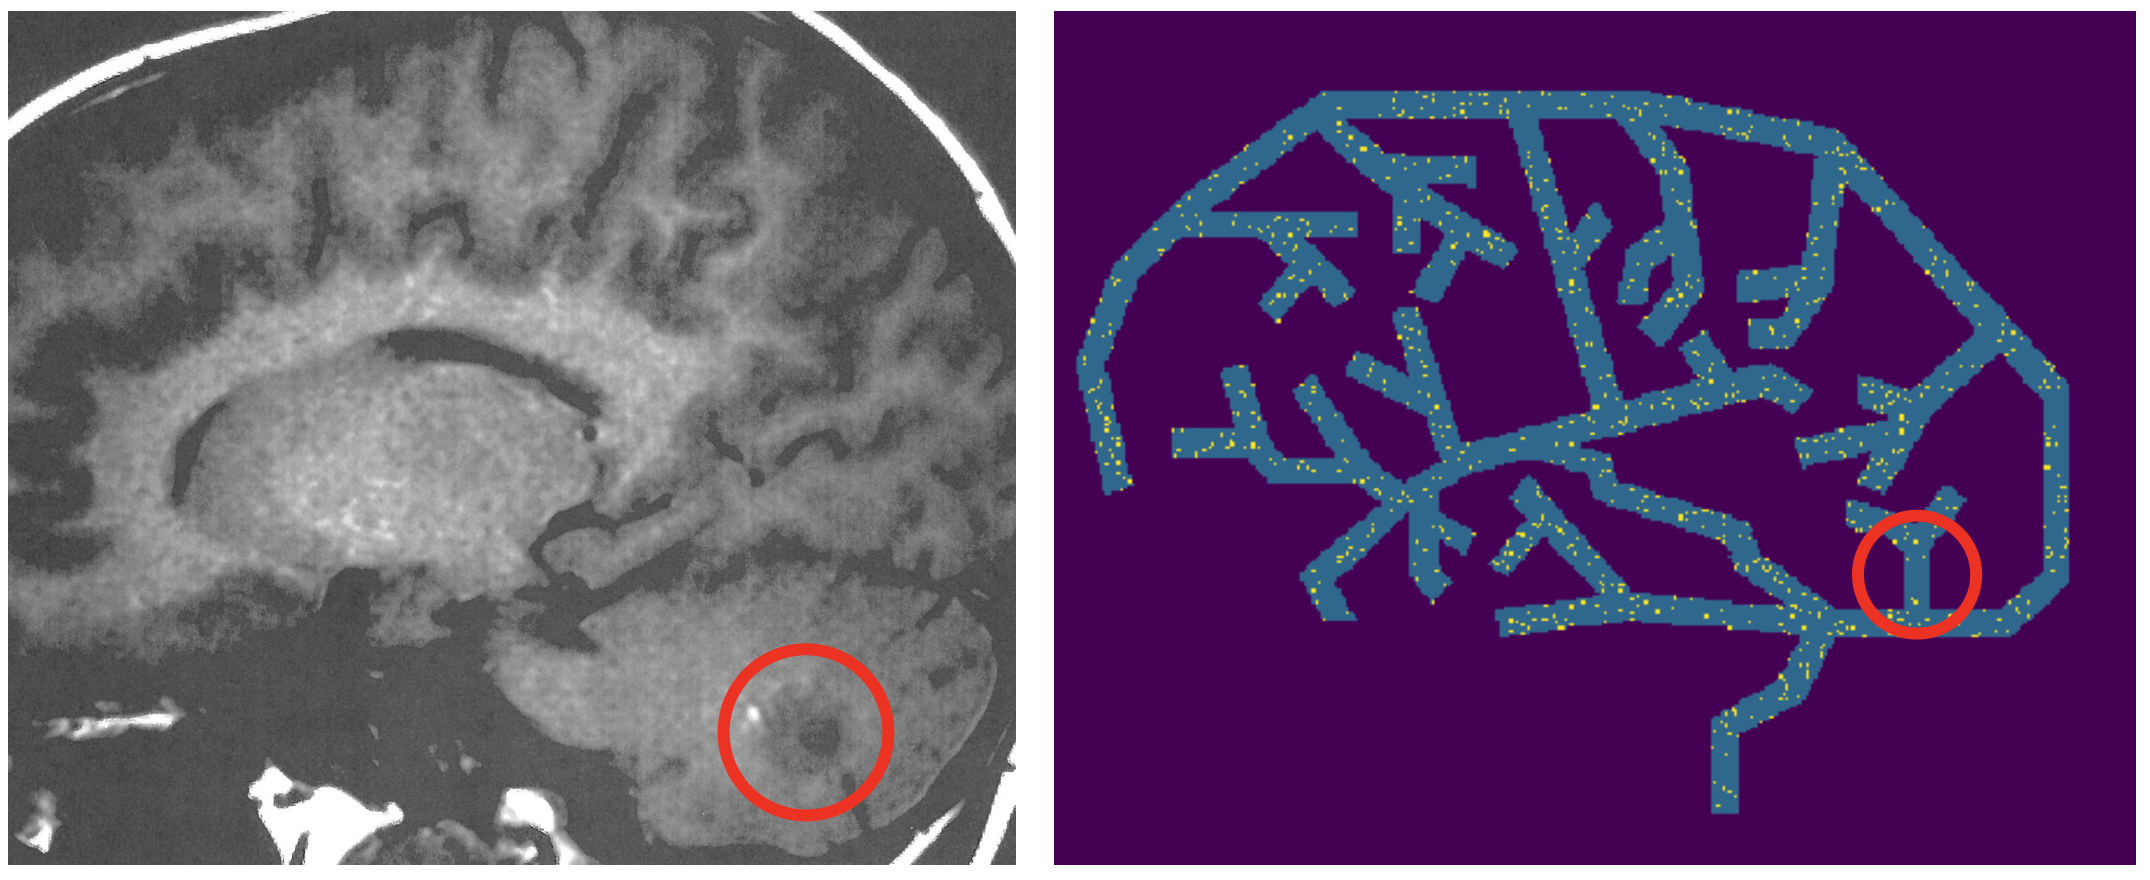
\includegraphics[clip, width=0.7\columnwidth]{figures/drugdelivery/brains.png}
    \end{center}
    
    %\vspace*{-6pt}
    \caption[Targeted Drug Delivery Motivation]{Targeted drug delivery for tumor treatment (from \cite{becker2020}). An MRI image on the right shows a tumor (marked by the red circle) and an abstracted version (left) shows particles containing some sort of medicine (yellow dots) which should be delivered to the target region.}
    \label{fig:brain_tumor}
    %\vspace*{-12pt}
\end{figure}

In 2020 it was proven by Becker et al. \cite{becker2020} that the navigation problem itself is NP-hard. This means, that approximation algorithms will be very important for any practical application. Becker et al. also showed, that it is possible to solve certain instances of the problem using reinforcement learning (RL) and that the resulting solution outperformed current approximation algorithms. While their approach delivered a proof-of-concept, it was computationally very heavy compared to the algorithmic approaches, as the RL algorithm needed millions of training steps before it could solve the problem. 
 
 Building up on this previous work, we want to improve the process of how RL algorithms can be used to solve this problem. Our goal is to speed up the learning process, train agents which generalize for multiple instances and investigate the possibilities of reinforcement learning to deal with extended settings which are closer to real-world targeted drug delivery. Our results may also be useful for the application of reinforcement learning on other algorithmic problems.

 \paragraph{Learning by Doing: Reinforcement Learning} 
In this work we will be using techniques from a specific field of machine learning called reinforcement learning or more specifically its modern combination with artificial neural networks called \textit{deep reinforcement learning}.

 Deep reinforcement learning is one of the most exciting fields of machine learning today, because it is capable of achieving actual superhuman performance without any human ever creating training data for it. In reinforcement learning the data is created solely by an agent interacting with its environment -- similar to how humans learn by trail and error. Deep reinforcement learning algorithms therefore are unsupervised machine learning algorithms.

 Like traditional machine learning, reinforcement learning has been around for decades, but just recently gained notable attention. In 2013 researchers from the British startup DeepMind were able to train a system to play any game from the game console Atari without prior knowledge and only with raw pixel data as input \cite{mnih2013playing}. They later even improved their system and were able to outperform trained human players \cite{mnih2015human}.These two successes were the beginning of a series of advances for deep reinforcement learning. In 2016 a team from Google DeepMind created a RL agent called \textit{AlphaGo} which was able to defeat multiple worlds top class Go players including the 2017 world champion Ke Jie \cite{borowiec2016alphago}. The system was later expanded to also play Shogi and Chess and renamed to \textit{AlphaGo Zero}. This new system gained notable attention, as it was able to defeated the state-of-the-art alpha-beta search engine for chess Stockfish \cite{silver2017mastering}. In 2019 they reached a new milestone, when their system \textit{AlphaStar} was able to beat a professional player at StarCraft II -- a complex multiplayer strategy game \cite{arulkumaran2019alphastar}. 

 All these advances were made possible by a number of breakthroughs in machine learning and reinforcement learning as well as an increase in computational power over the last decade. The victory of AlphaGo Zero over its algorithmic competitor Stockfish also demonstrates how RL algorithms can be used as a replacement for algorithmic solutions in completely new areas of computer science. 


\section{Previous and Related Work} \label{sec:RelatedWork}
In this thesis, we want to use reinforcement learning to train neural networks to steer large numbers of microrobots or microscopic particles through a maze-like environment to a goal position. In a real-world scenario this maze-like environment may be the blood vessels in a human body, and the target position may be a tumor. 

To date, we already have the possibility to create particles which contain a magnetic core and have a catalytic or biodegradable surface which allows them to release their payload at the target position \cite{litvinov2012high, mellal2015magnetic}. To navigate these particles through the blood vessels, magnetic fields produced by modified gradient coils inside of an MRI scanner can be used \cite{mathieu2007magnetic, mathieu2010steering}. The scanner can also be used to provide real-time feedback and track the position of the nanoparticles \cite{pouponneau2009magnetic}. Since blood vessels build a complex system of paths, directing the particles to the goal position requires efficient motion planning algorithms. 

Controlling a larger number of particles by global inputs has been studied in very different settings in the past. Assembling complex shapes using a swarm of particles was explored in \cite{becker2018tilt} and \cite{balanza2019full}. Often it is not required to bring the particles to a goal position, but to rearrange them in a certain way, which has been done in \cite{becker2013massive} and \cite{zhang2017rearranging}. 

Moving particles to a goal position is directly related to another problem studied in the past called \textit{rendezvous search} \cite{alpern2006theory}. Rendezvous search aims at finding a sequence of movements for two or more independent agents to meet at the same location. Since it is easy to move a single particle (or a number of particles concentrated at a single point) to the goal position via the shortest available path, we can express our problem by a sequence of rendezvous between particles, ultimately gathering all particles at a single location.

 Early algorithmic approaches and settings were introduced by Alpern and Gal \cite{alpern2006theory} as well as by Anderson and Fekete \cite{anderson2001two}. Their work included agents with limited onboard computations, but in certain cases both agents followed the same movement protocol -- executing the same movement. The problem can therefore also be called \textit{symmetric} rendezvous search where the symmetry is only broken by interaction with obstacles. Since all agents perform the same movements, this directly corresponds to the particle navigation problem. 

Rendezvous search was extended into a sequence of rendezvous to collect a swarm of particles in a single place by Mahadev et al. \cite{mahadev2016collecting}. Just recently it was proven, that computation of an optimal gathering sequence is NP-hard \cite{becker2020}. The authors also proposed several new approximation algorithms, including an approach for the application of reinforcement learning \cite{huang2019, becker2020}. Even though the reinforcement learning approach is computationally more expensive, it produces much shorter gathering sequences.

In their approach, Becker et al. used recent techniques to train the RL agent. To improve training, they included an intrinsic reward signal, guiding the agent to explore "interesting" environment states. This technique was explored for a long time to supplement sparse extrinsic rewards \cite{pathak2017curiosity, mohamed2015variational, houthooft2016variational} and recently found notable attention with the introduction of the \textit{intrinsic curiosity module} \cite{burda2018large} and the \textit{random network distillation} methods \cite{burda2018exploration}. The latter uses prediction error to simulate real intrinsic motivation. Both techniques have shown to drastically improve performance on "hard" games from the Atari game suite when used in combination with the well-known trust region optimization technique \textit{proximal policy optimization} \cite{schulman2017proximal}. Just recently, Baida et al. presented an improved curiosity signal which has shown to work exceptionally well even in the presence of extremely noise maze-like environments \cite{badia2020never}.

\section{Our Results} \label{sec:Results}
To evaluate reinforcement learning (RL) algorithms, we implemented a laboratory environment for RL agents called Baselines Lab. We also implemented a high-performance simulation for the particle navigation problem. Using these two components in a series of experiments, we provide a number of insights on improving the performance of RL agents on the distributed particle navigation problem:

\begin{itemize}
    \item We provide a novel continuous reward to guide RL agents in environments with distributed particles which accelerates training (see Section \ref{sec:MazeReward} and Section \ref{sec:EvalReward}).
    \item We perform an extensive study on different rewards, including previous goal-based reward, our continuous reward and combinations with intrinsic curiosity reward (see Section \ref{sec:EvalReward}).
    \item We perform a study on the performance of different RL algorithms and provide a set of optimized hyperparameters for each of them (see Section \ref{sec:EvalRLAlgorithms}).
    \item We perform a study on observation preprocessing, including observation downscaling (see Section \ref{sec:Eval/ObsSize}) and frame stacking (see Section \ref{sec:EvalObs}).
    \item We analyze the impact of different structures for neural networks and used activation functions (see Section \ref{sec:Eval/NetworkStructure}).
    \item We provide a new baseline for the performance of RL agents together with a comparison with previous RL and algorithmic approaches (see Section \ref{sec:EvalBaseline}).  
\end{itemize}

\noindent Additionally, we studied the impact on training performance when introducing additional real-world problems:

\begin{itemize}
    \item We show that RL agents are capable of dealing with simplified physical particle behavior (see Section \ref{sec:EvalPhysical}).
    \item We show that RL agents are able to deal with a certain amount of observation error, including random noise and false positive and negative detection of particles (see Section \ref{sec:EvalError}).
    \item We show that RL agents are also able to deal with a certain amount of action error, including repeated (sticky) actions, partially random actions and actions which only affect a random number of particles. (see Section \ref{sec:EvalError}). 
\end{itemize}

\noindent Finally, we made advances in generalizing agent behavior for more than a single instance:

\begin{itemize}
    \item We show, that agents are able to learn strategies which can gather particles at random goal positions for a single maze instance (see Section \ref{sec:EvalRandomGoals}).
    \item We show that agents are able to learn strategies which can gather particles at random goal positions for multiple small instances (see Section \ref{sec:EvalRandomMaze}).
\end{itemize}


\chapter{Guiding Particle Swarms with Global Force} \label{chp:TDD}
In this chapter we want to give an introduction into the problem which we will later try to solve using reinforcement learning. Controlling large particle swarms with a global force is a challenging navigation problem. Particles can either be partially autonomous robots, which move in unison into a direction given by an external signal (e.g. a light source), or the particles can be without any autonomy where we have a global force like magnetism which controls their movement. Because particles can be seen as marbles on a surface which are controlled by tilting, the problem is often referred to as tilt problem. Depending on the task there are a number of goals which can be solved in this setting, e.g. the well-known tilt assembly problem, where the goal is to build objects using particles controlled by a global force \cite{becker2018tilt}. In this work we will focus on another problem, which finds its application in medicine and aims at navigating particles to a specific goal position inside of the human body. We will give a more detailed introduction in Section \ref{sec:TDDMotivation}. We will then continue with a theoretical point of view on the problem in Section \ref{sec:TDDPreliminaries} and present a number of existing algorithmic approaches to solve the problem in Section \ref{sec:TDDPreviousWork}. We will finally present previous work on solving the problem with reinforcement learning in Section \ref{sec:TDDRL}. 

\section{Motivation} \label{sec:TDDMotivation}
The treatment of medical problems often requires the use of some sort of medication. These medications are given as oral ingestion or intravascular  injection and then are further distributed throughout the body via blood circulation. Most if not all of these treatments can produce some potentially serious side-effects. Especially when treating serious medical problems like internal bleedings, localized infections, tumors or cancer (see Figure \ref{fig:brain_tumor}), a large portion of the medication does not reach its target destination and the possible worst-case side-effects can be as serious as the original medical problem. The idea of \textit{targeted drug delivery}, deals with the problem to concentrate some given medicine in a certain part of the body to reduce unwanted side-effects and at the same time increase the efficacy.

\begin{figure}[ht]
    
    \begin{center}
        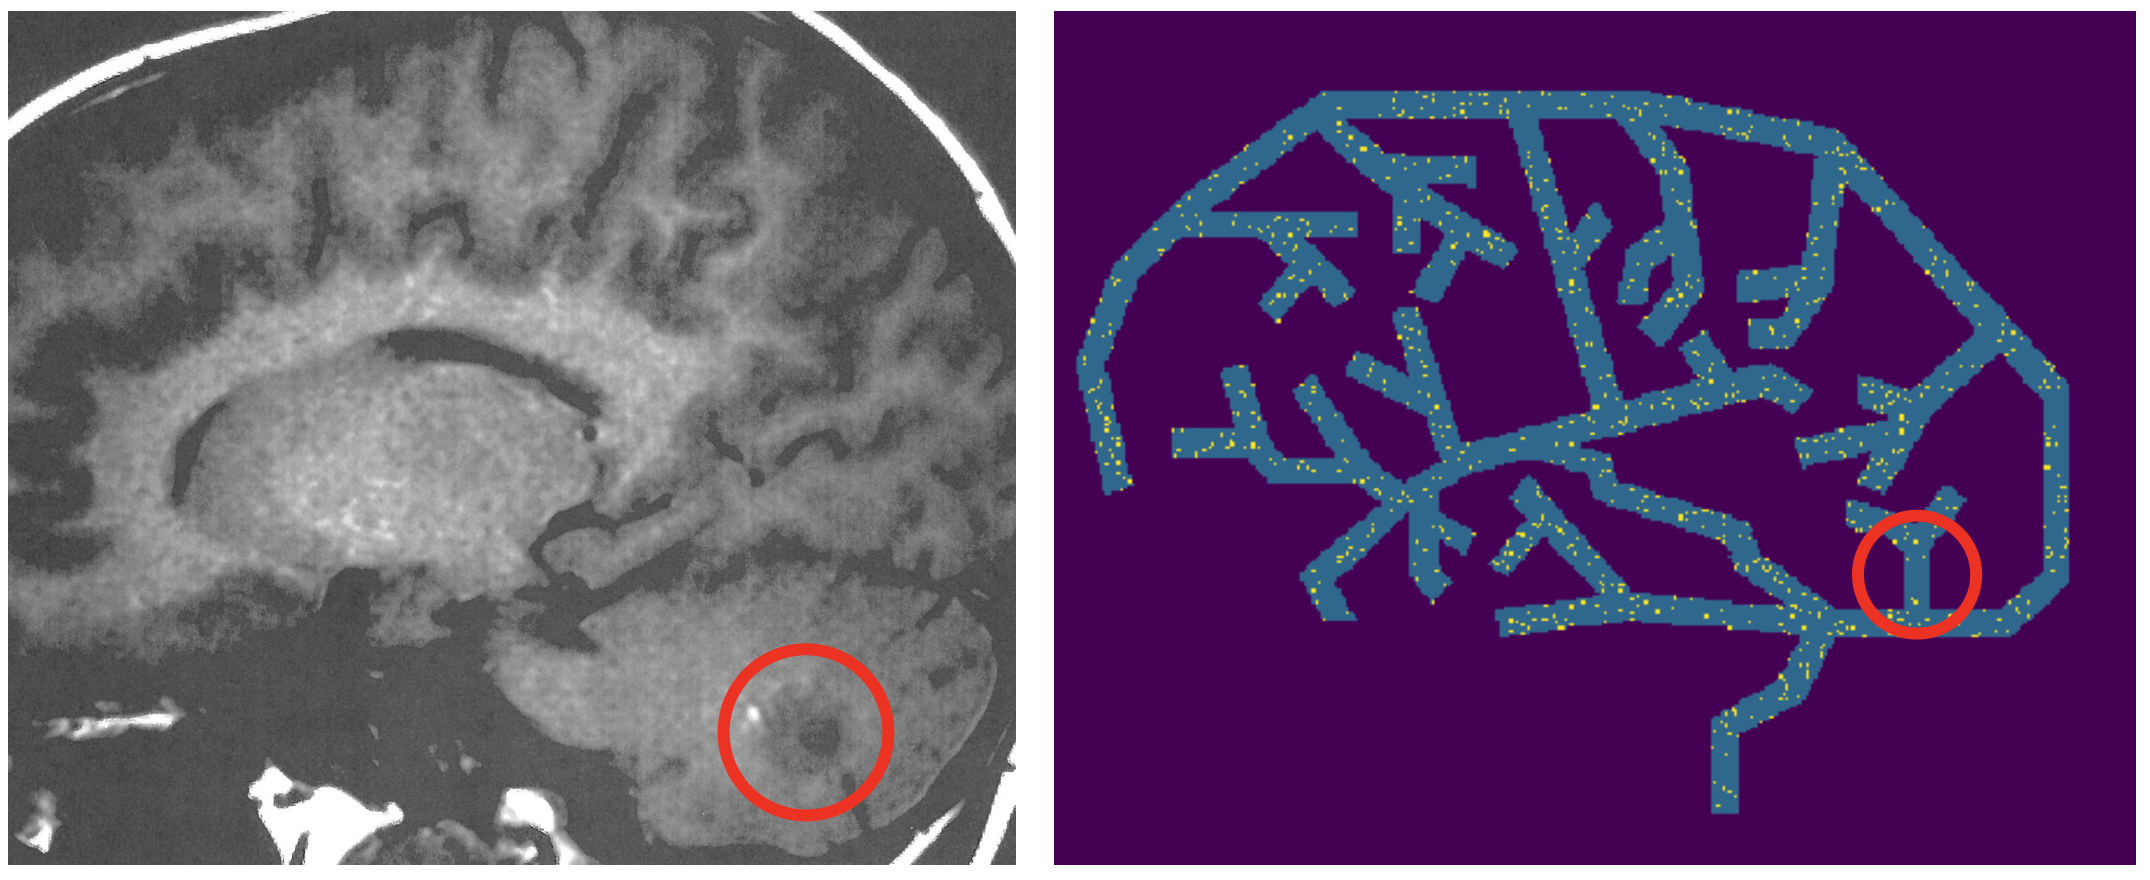
\includegraphics[clip, width=0.7\columnwidth]{figures/drugdelivery/brains.png}
    \end{center}
    
    %\vspace*{-6pt}
    \caption[Targeted Drug Delivery Example]{Targeted drug delivery for tumor treatment (from \cite{becker2020}). An MRI image on the right shows a tumor (marked by the red circle) and an abstracted version (left) shows particles containing some sort of medicine (yellow dots) which should be delivered to the target region.}
    \label{fig:brain_tumor}
    %\vspace*{-12pt}
\end{figure}

Over the years many approaches have been developed to perform targeted drug delivery. In recent work, the idea of using magnetic nanoparticles has been explored and proven to be promising, since they combine high drug loading with great targeting abilities \cite{vangijzegem2019magnetic, albinali2019perspective}. The particles are controlled by an external uniform magnetic force and guided towards a target location. The magnetic fields can be generated by using the coils in an MRI scanner \cite{mathieu2007magnetic, pouponneau2009magnetic} or by adding additional magnetic coils \cite{mellal2015magnetic}. Real-time MRI scanning also allows feedback control to some extend. At their target location, the particles are activated to release their payload by an external or internal stimulus such as temperature or pH.

Guiding particles by a uniform external (\textit{global}) force requires solving a complex distributed navigation problem. The nanoparticles will be distributed randomly in a complex maze-like environment given by the vascular system of blood vessels. Using a uniform force to guide all particles regardless of their initial position to a single destination will be complicated due to many particles being blocked at some point by obstacles. This problem has been studied in the past in terms of bringing two particles to the same location called \textit{rendevous search}. In 2001 Anderson and Fekete introduced methods for two-dimensional rendevous search \cite{anderson2001two} and Alpern and Gal introduced a number of new settings along with solution strategies in their 2006 paper \cite{alpern2006theory}. However in this chapter we want to focus on a more recent work by Becker et al. \cite{becker2020} from 2020. They prove that the underlying problem is NP-hard and also present some novel approximation algorithms which greatly improve previous worst case guarantees.


\section{Preliminaries} \label{sec:TDDPreliminaries}
Using particles with individual capabilities (e.g. microrobots) is difficult since the tiny volume of these robots makes it nearly impossible to store enough energy to navigate in presence of flowing blood. The particles we are dealing with therefore have no computational power, memory or any other autonomy. Instead our particles are just some kind of substrate (e.g. iron-oxide) injected into the blood vessels and solely controlled by a uniform global force which affects all particles equally. In our model we will work with a two-dimensional abstraction of the environment and the particles: The blood-vessels will be modeled by a planar two-dimensional integer workspace $P$ which consists of orthogonal cells (\textit{pixels}) and can therefore be seen as \textit{polyomino}. All pixels not belonging to the polyomino are blocked and cannot be entered by particles. The distance $dist(p, q)$ between two pixels $p$ and $q$ is given by the shortest path on the integer grid between $p$ and $q$ that stays within $P$. The diameter $D$ of the polyomino is then given by the maximum distance between any two of its pixels. 

At the beginning, each pixel of $P$ may contain one (or more) particles which we will call the \textit{configuration} of $P$, with the set of all possible configurations $\mathcal{P}$. Since we are dealing with edge-to-edge connected cells, four basic moves are possible to move each particle by one cell in one of the directions "Up" (\textit{u}), "Down" (\textit{d}), "Left" (\textit{l}) or "Right" (\textit{r}). If the particle cannot move to the next cell because it is blocked, it simply remains in its current cell. Since the size of the particles is insignificant compared to the size of the cells, if two particles $a$ and $b$ enter the same cell $p$, they will merge into a single particle. This can happen when $a$ enters $p$, while $b$ remains in $p$ due to being blocked. Merged particles will never be separated again and move in unison for subsequent moves.

We call a series of commands a \textit{motion plan} $C = \langle c_1, c_2, c_3, \dots \rangle$ where each command $c_i \in \{u, d, l, r\}$. We further call a command sequence \textit{gathering} if it merges all particles of a given configuration $A \in \mathcal{P}$ into a single pixel, such that $|A'| = 1$.


\section{Algorithmic Approaches} \label{sec:TDDPreviousWork}
In this Section we want to present a number of algorithmic approaches to solve targeted drug delivery. To keep things short, we will focus on recent algorithms which provide a reasonably good performance bound and have proven to perform at least as good as previous approaches. All algorithmic approaches use a gathering strategy, which first concentrates all particles into a single cell. The particles are then guided to the target area on a shortest path.

\subsection{Static Shortest Path}
In 2016 Mahadev et al. developed a simple greedy algorithm which is able to collect all $m$ particles with a command sequence of length $\mathcal{O}(m \cdot n^3)$, where $n$ is the polyomino's height times its width \cite{mahadev2016collecting}. The algorithm was later named \textit{Static Shortest Path} (SSP) in a paper by Becker et al. \cite{becker2020}. 

\begin{algorithm}[ht]
    \KwData{Configuration $A$, Bounded polyomino $P$}

    \While{$|A| > 1$}{
        Select two particles $a$ and $b$ from $A$. \;
        \texttt{StaticShortestPath}($a$, $b$)
    }

    \SetKwProg{Merge}{procedure}{:}{}
    \Merge{\texttt{StaticShortestPath} ($a$ : Particle, $b$: Particle)}{
        \While{$dist(a, b) \neq 0$} {
        Compute $C \in \{u, d, l, r\}^N$ as the shortest control sequence to move $a$ onto $pos(b)$. \;
        Execute $C$.
        }
    }
    
    \caption[Static Shortest Path Algorithm]{The static shortest path algorithm modified to merge an arbitrary number of particles.} \label{alg:SSP}
\end{algorithm}

The algorithm works by iteratively merging two particles until all particles are merged into a single one. We included a sketch in Algorithm \ref{alg:SSP}. We can see, that the algorithm uses the procedure \texttt{StaticShortestPath}, which subsequently moves a particle $a$ to the position of another particle $b$ until they are merged. Mahadev et al. showed, that when moving $a$ to the position ob $b$, the distance between the particles $a$ and $b$ only decreases if $b$ had a collision. Since the polyomino is bounded and $a$ and $b$ always move into the same direction, $b$ must have a collision after $\mathcal{O}(n)$ collision free iterations. Therefore $\mathcal{O}(n^2)$ commands are needed to reduce the distance by at least one, resulting in $\mathcal{O}(n^3)$ commands in total to merge two particles. The choice of particles that are merged in the next step can be random, but it has been shown, that choosing the pair with the maximal distance converges faster on average.

\subsection{Dynamic Shortest Path}
In 2020, Becker et al. presented a number of improved algorithms which provide stronger performance bounds \cite{becker2020}. For the special case of hole-free polyominos, they developed the \textit{Dynamic Shortest Path} (DSP) algorithm which is able to compute a gathering sequence of $\mathcal{O}(D)$ with $D$ being the diameter of the polyomino. For non-simple polyominos, DSP still always merges two particles, but may need $\mathcal{O}(nD)$ steps, where $n$ is the number of pixels in the polyomino. 

\begin{figure}[ht]
    
    \begin{center}
        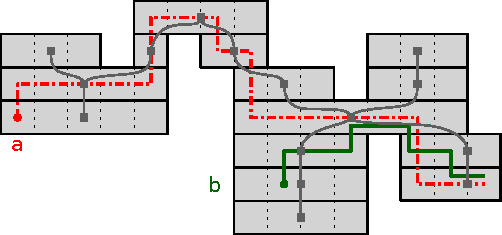
\includegraphics[clip, width=0.6\columnwidth]{figures/drugdelivery/Gathering_Simple_b.pdf}
    \end{center}
    
    %\vspace*{-6pt}
    \caption[DSP and the Edge Contact Graph]{A simple polyomino $P$ and its edge-contact graph $\mathcal{C}(R)$. The particle $a$ (red) is moved towards particle $b$ (green) on a shortest path with respect to $\mathcal{C}(R)$. (from \cite{becker2020}, edited)}
    \label{fig:edge_contact_graph}
    %\vspace*{-12pt}
\end{figure}


\begin{algorithm}[ht]
    \KwData{Configuration $A$, Bounded polyomino $P$}

    \While{$|A| > 1$}{
        Select two particles $a$ and $b$ from $A$. \;
        \texttt{DynamicShortestPath}($a$, $b$)
    }

    \SetKwProg{Merge}{procedure}{:}{}
    \Merge{\texttt{DynamicShortestPath} ($a$ : Particle, $b$: Particle)}{
        \While{$R^a_t \neq R^b_t$} {
            Compute a shortest path $S_t$ from $R^a_t$ to $R^b_t$ in $\mathcal{C}(R)$ \;
            Move $a$ to $S_t(1)$ via a shortest path in $P$. \;
            Update $R^a_t$ and $R^b_t$
        }

        Compute a shortest path $C$ from $a$ to $b$. \;
        Merge $a$ and $b$ by executing $C$.
    }
    
    \caption[Dynamic Shortest Path Algorithm]{The dynamic shortest path algorithm modified to merge an arbitrary number of particles.}\label{alg:DSP}
\end{algorithm}

The DSP algorithm starts by decomposing $P$ with horizontal lines through pixel edges which results in a set of rectangles $R$. The edge-contact graph $\mathcal{C}(R)$ is then constructed by creating a vertex for each rectangle and connecting two vertices if their respective rectangles share an edge. For a simple (hole-free) polyomino the edge-contact graph is a tree. Two particles are then merged by using an improved shortest path strategy. For two particles $a$ and $b$, let $R^a_t$ and $R^b_t$ be the rectangles of $P$ containing the two particles in step $t$. Let $S_t$ be a shortest path from $R^a_t$ to $R^b_t$ and let $S_t(1)$ be the successor of $R^a_t$ on $S_t$ if it exists ($R^a_t \neq R^b_t$). The particles are then merged, by subsequently moving $a$ on a shortest path from $R^a_T$ to $S_t(1)$ and then recalculating $S_t$ (therefore the name \textit{dynamic} shortest path). If there is no $S_t(1)$ the particles are merged, by moving $a$ towards $b$ by a shortest (horizontal) path, merging both particles within $R^a_t$. The whole process can be found in Algorithm \ref{alg:DSP} and an example showing the edge-contact graph and the process of merging two particles is shown in Figure \ref{fig:edge_contact_graph}.


\subsection{Move to Extremum}
The strategy \textit{Move to Extremum} (MTE) was also developed by Becker et al. \cite{becker2020} and provides a strategy which - independent of the shape of the polyomino - provides a gathering sequence of length at most $\mathcal{O}(D^2)$ for two particles. The idea of MTE is to iteratively move an extreme particle (e.g. the top-rightmost) to an opposite extremum (e.g. bottom-leftmost) along a shortest path. Similar to the shortest path approach in SSP, the distance then decreases with every iteration. 

Let $q$ be the top-rightmost pixel of $P$. To merge two particles, we select the bottom-leftmost particle $a$ and compute a sequence of moves, which moves $a$ to $q$ on a shortest path. We repeat this procedure of selecting the bottom-leftmost particle and moving it to $q$ until the particles have been merged. In each iteration, the sum of distances $\Delta$ of the two particles to $q$ decreases. This happens only if the other particle $b$ has a collision. Similarly to SSP, in every iteration the particle $b$ must have at least one collision (otherwise $q$ could not be the top-rightmost pixel or $a$ not the bottom-leftmost particle), so the sum decreases at least by 1 every $D$ steps. Since in some polyominos (e.g. a square), the number of pixels $n$ is in $\Omega (D^2)$, we can argue, that the MTE produces sequences which are significantly shorter than $\mathcal{O}(n^3)$ from SSP.

\begin{algorithm}[ht]
    \KwData{Configuration $A$, Bounded polyomino $P$}
    
    Determine which of the four corner types occurs at most $k/4$ times. \;
    Apply a sequence of commands to merge all particles into at most $k/4$ groups.

    \While{$|A| > 1$}{
        Calculate the sum of distances for all particles $d_t$ for each extremum. \;
        For each command calculate the change in the sum of distances $\Delta d_t^{c_i}$ that command would produce. \;
        Select the command $j$ which decreases the sum the most. \;
        \eIf{$\Delta d_t^{c_j} < 0$}{
            Execute $j$
        }{
            Select two particles $a$ and $b$ from $A$. \;
            \texttt{MoveToExtremum}($a$, $b$)
        }
    }

    \SetKwProg{Merge}{procedure}{:}{}
    \Merge{\texttt{MoveToExtremum} ($a$ : Particle, $b$: Particle)}{
        Select an extremum $q$ which minimizes the sum to $a$ and $b$. \;
        \While{$dist(a, b) \neq 0$} {
            Select the particle which is further away from $q$. \;
            Move that particle to $q$ on a shortest path. \;
        }

    }
    
    \caption[The Min Sum To Extremum algorithm]{The min sum to extremum algorithm to gather all particles. MTE is used as a subroutine and particles are merged into $k/4$ groups in convex corners at the beginning to reduce their total number.}\label{alg:MSTE}
\end{algorithm}

If we look at a swarm of particles, we can have at most $n$ individual particles in any configuration of a polyomino $P$, which would result in a total of $\mathcal{O}(nD^2)$ commands for a gathering sequence using MTE. Luckily, it is possible to further reduce the total number of particles by first moving them into convex corners. For every polyomino with $k$ convex corners, a diameter $D$ and a configuration $A \in \mathcal{P}$, this can be done with a command sequence of length $2D$. The resulting configuration $A' \in \mathcal{P}$ will have at most $k/4$ particles. This works by first selecting the type of convex corner from all convex corners (northwest (NW), northeast (NE), southwest (SW) and southeast (SE)) which occurs at most $k/4$ times. It is guaranteed by the pigeon hole principle that such a convex corner type must exist. Let us assume the NE corner is the type selected. After applying a sequence of $\langle r, u \rangle^D$ every particle lies in a NE corner. Therefore the total gathering sequence of MTE has a length of $\mathcal{O}(kD^2)$. 

In their paper, Becker et al. also propose a variant of MTE called \textit{Min Sum To Extremum} (MSTE) which generalizes the idea of MTE for a swarm of particles. Initially, MTE selects an extremum which has the smallest sum of distances to all particles. It then tries to find a command which reduces this sum the most. If it is unable to find such a command, it continues by merging two particles using regular MTE. We provide pseudocode for MSTE which also includes MTE as a subroutine in Algorithm \ref{alg:MSTE}. The particles are gathered into $k/4$ groups at the beginning.

\section{The Reinforcement Learning Approach} \label{sec:TDDRL}
In 2019 Li Huang showed that is is possible to solve the targeted drug delivery problem with reinforcement learning \cite{huang2019}. His approach was later tested against the algorithmic approaches and proved to significantly outperform both MTE and MSTE on individual instances \cite{becker2020}. In this section, we want to give an overview over how the agents for targeted drug delivery can be trained. The methods and terminology which are used for this approach will be explained in detail in Chapter \ref{chp: RLOverview}.

\begin{figure}[ht]
    
    \begin{center}
        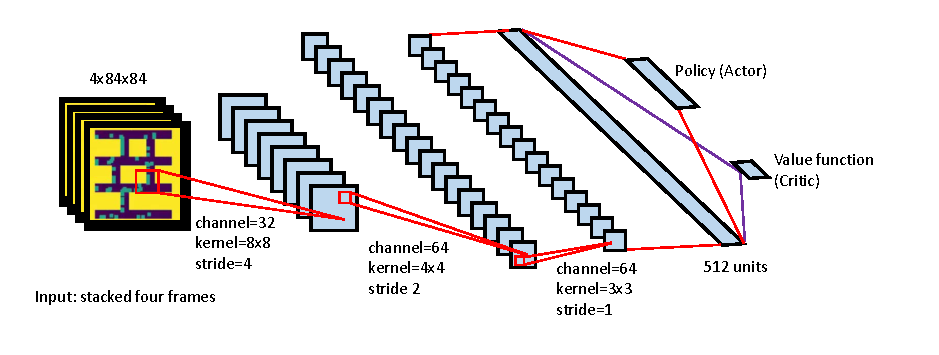
\includegraphics[clip, width=0.95\columnwidth]{figures/drugdelivery/Network_Architecture.pdf}
    \end{center}
    
    %\vspace*{-6pt}
    \caption[Network Architecture for the RL Approach]{The network architecture for the reinforcement learning approach (from \cite{huang2019}).}
    \label{fig:huang_network_architecture}
    %\vspace*{-12pt}
\end{figure}

\paragraph{The Particle Maze Environment.}
For reinforcement learning every problem has to be modeled as an environment where the agent can take actions and from where it receives observations and reward in return. For the problem of gathering particles at a goal location, the environment represents a single instance of the targeted drug delivery problem (a single polyomino) with a single target position. Particles are randomly spawned in empty cells of the polyomino at the beginning of an episode and the episode ends if all particles reach the goal position or after a certain time limit. Observations are generated as a visual representation of the environment as a grayscale image. The image includes the shape of the polyomino and the position of each particle. The observation will the be further preprocessed by downscaling the image to $84 \times 84$ pixels. Additionally the network receives a stack of the last four frames to add information about past particle positions. Images are also normalized by their variance and zero centered with precomputed values from a random agent playing 10000 steps.

For reinforcement learning, the reward signal is a crucial component. Even a simple problem might become very hard to learn for an agent if the reward signal does not provide enough information about the goal or if it is somehow inconsistent or extremely sparse. Huang et al. generated reward based on a set of predefined goals. There are two main categories for these goals: The maximum distance of any particle to the goal position and the average distance of all particles to the goal position. In each category, the agent receives rewards based on reaching certain milestones - e.g. if the particle with the largest distance to the goal is less than 50 cells away from the goal position, the agent is granted a reward of $+2$. Rewards may increase for higher goal tiers and are only granted a single time for each episode. If the agent is able to bring all particles to the goal position it receives a large final reward of $+100$. The goals that were used during the experiments were sparse and limited to only 4-8 distinct rewards in each category. Rewards are also not normalized.

\begin{table} [ht]
    \begin{center}
        \begin{tabular}{|p{6.5cm}|c|}
            \hline
            Hyperparameter & Default Value \\
            \hline
            Extrinsic Reward Clipping & False \\
            Extrinsic Reward Normalization & False \\
            Intrinsic Reward Clipping & False \\
            Intrinsic Reward Normalization & True \\
            Steps Per Episode & 2048 \\
            Total Steps & 2e8 \\
            Number of Minibatches & 16 \\
            Number of optimization epochs & 4 \\
            Extrinsic Reward Coefficient & 1.0 \\
            Intrinsic Reward Coefficient & 0.5 \\
            Number of Environments & 128 \\
            Learning Rate & 0.0001 \\
            Entropy Coefficient & 0.001 \\
            \hline
        \end{tabular}
    \end{center}
    \caption[RL Approach Default Parameters]{Default parameters for PPO with RND curiosity rewards as used in the reinforcement learning approach on the targeted drug delivery problem by Huang and Becker et al. \cite{huang2019}.} \label{tab:RLDefaults}
\end{table}

\paragraph{The Targeted Drug Delivery Agent}
The agent for the targeted drug delivery problem is inspired by the agent used for the large scale study on curiosity learning by Burda et al. in 2018 \cite{burda2018large}. Since the targeted drug delivery problem requires careful exploration of the environment, the agent heavily profits from the addition of a curiosity reward. For reward generation the original methods from \cite{burda2018large} were used, as well as the random network distillation method (see Section \ref{ssec:Curiosity}). RND showed superior performance in all experiments which were done with both rewards. 

The agent itself is build with an actor-critic architecture and trained using the PPO algorithm (see Section \ref{ssec:PPO}). The neural network uses convolutional layers to process the image information (see Section \ref{ssec:CNNs}) and follows the frequently used natural CNN design. The architecture can be found in Figure \ref{fig:huang_network_architecture} and consists out of four convolutional layers with 32 ($8\times 8, s=4$), 64 ($4\times 4, s=2$) and 64 ($2\times 2, s=1$) filters which are then connected to a single fully connected layer with 512 neurons. The original four commands used to move the particles are extended by another four additional commands. Rather than just using "North" (up), "South" (Down), "West" (Right) and "East" (Left), the agent also is allowed to also use "Northwest", "Northeast", "Southwest" and "Southeast" as movement commands. Additional training parameters for PPO and curiosity can be found in Table \ref{tab:RLDefaults}.

The reinforcement learning approach proved to have exceptionally good performance on single (small) instances, but is costly due to the long training process. Huang et al. showed, that PPO was not able to successfully solve instances by using the extrinsic reward signal only. Even after extremely long training sessions with over 3 billion timesteps, PPO was not able to solve a single instance. The addition of the intrinsic curiosity reward solved this problem, by dramatically decreasing training time and leading to positive results even for larger and more complex instances.


\chapter{Deep Learning} \label{chp:DeepLearning}
This chapter summarizes the fundamentals of machine learning with a special focus on artificial neural networks. We will take a look at how these networks are built and how they can be trained. The term \textit{Deep Learning} actually refers to the structural size of these artificial networks in modern applications which are build from tens to hundreds of layers. \\
We will begin with some basic motivation and get familiar with terms and notation for machine learning in Section \ref{ssec:MLNutshell}. We then dive into the world of artificial neural networks and how they can be trained in Section \ref{sec:ANNs}, where we also talk about some of the most challenging problems for nowadays architectures and how they can be solved. Finally we will finish with some specialized network structures for specific applications in Section \ref{sec:SpecializedNetworks}.

\section{Machine Learning in a Nutshell} \label{ssec:MLNutshell}
In this Section we want to give an introduction into machine learning. We will begin with some motivation and talk about why machine learning matters in Section \ref{ssec:MLMotivation} and follow up with some basic terms and notation in Section \ref{ssec:MLNotation}.

\subsection{Motivation} \label{ssec:MLMotivation}
Before we dive into neural networks, let us briefly talk about what machine learning is and what makes it special. Machine learning is a field of study of computer science, which tries to give computers the ability to solve a task without a human writing an explicit algorithm for it. Usually machine learning works by providing \textit{training data} to a specialized learning algorithm which will then try to solve a task by optimizing a performance measure. For example think about a set of images, where on some of the images show apples and others show pears. When training, we split our \textit{dataset} into two - a larger one which will be our \textit{training dataset} and a smaller one which will be our \textit{test dataset}. Our algorithm will learn with the images from the training dataset only and for each sample gets the information what it can expect to see on the image. Its progress is then measured periodically in terms of \textit{accuracy} on the test dataset.

While we can expect a learned model to be fairly good, we can also expect to never reach a 100\% accuracy. Additionally machine learning is hard and time consuming so why do we not use traditional algorithms? Well first of all because there are many problems where traditional algorithms are either too complex or it does not even exist an algorithm to solve them. For example there is no known algorithm which precisely recognizes and classifies objects in an image. Machine learning can also be very dynamic. Imagine a spam detection engine. Traditional approaches worked with keyword filters which were simply lists of forbidden words (or sentences) created by humans. This approach required a lot of tedious work for a result which is not very robust, since someone who knows the filter list can try to simply use different words. In a setting where we use machine learning, we could let the computer create this list on its own. The only thing we would need to do is to tell it, which email contains spam and which does not. Machine learning can also go a step further and build a language model for us which allows to automatically detect synonyms - improving the robustness of the learned list. 

Machine learning is not only great at solving complex tasks, it can also help humans to learn. Machine learning is a great tool to find information in big piles of raw data. This area is called \textit{data mining} and can help to find unknown patterns to better understand problems.

\subsection{Terminology and Notation} \label{ssec:MLNotation}
In this Section we want to introduce some basic notation and terminology from the area of machine learning. We will further try to get a better view on what machine learning is from a mathematical point of view.

\paragraph{Types of Machine Learning.} Machine Learning is a very broad area and - depending on the task - very different techniques will be used.Therefore learning algorithms can usually be divided in (at least) three main categories:

\begin{enumerate}
  \item \textit{Supervised Learning.} Supervised learning algorithms aim at building a model from a training dataset where for each sample in the training dataset the desired output is given. Typical uses are classification or regression tasks.
  \item \textit{Unsupervised Learning.} Unsupervised learning algorithms try to find structure in a given dataset without the desired output. They are often used for clustering which is done by exploiting some similarity metric. Unsupervised methods can often be combined with supervised methods and then are called semi-supervised methods.
  \item \textit{Reinforcement Learning.} Reinforcement learning tries to train an agent to take actions in an environment to reach a certain goal. The agent is usually guided by some reward given to it which it will try to maximize. We will take a detailed look at reinforcement learning in Chapter \ref{chp: RLOverview}.
\end{enumerate}

\paragraph{Data Representation.} Data is not only a central element for every computer system, but also highly important for any machine learning algorithm. Without data, there is nothing we can learn from. Data can have arbitrary origin, but if the data comes from the real world it is usually collected by sensors. The data is often preprocessed and the algorithm gets the data in form of a vector representation $\mathbf{x} \in \mathbb{R}^n$ which we call the \textit{feature vector} $\mathbf{x}$ in the \textit{feature space} $\mathbb{R}^n$. These terms originate from the idea, that each dimension of the vector may contain a certain feature (e.g. weight and color of a fish), but we can also work on "raw" features like the values of pixels in an image. If we have a set of feature vectors (samples), we denote the whole set by $\mathbf{X}$. Data is crucially important for the performance of the model. The best algorithm will not be able to create a good model from a bad dataset. In particular datasets may be too small or unrepresentative to model a real distribution, the dataset might be be biased towards or against a certain group, or the samples of the dataset may not be independent which makes it hard to learn from them. Gathering good training data is therefore a central problem of machine learning.

\paragraph{Machine Learning Models.}
To solve a given task, machine learning algorithms build a model which is trained using the training data. We call a model which is done with its training process an \textit{inference} model, which is then used at \textit{test time} to solve the problem it has been trained for. There are currently a number of different models available, most prominent the artificial neural networks which we will discuss in the remainder of this chapter, but there are also other kinds of models like \textit{decision trees} or \textit{support vector machines}. All models are in some way parameterizable and we will denote their parameters with $\theta$. Depending on the task, models have a specific output, which is usually also in vector form and denoted by $\mathbf{y}$. For example if we look at classification tasks, the output vector usually contains probabilities for each class $i$. The model can then be seen as a function which outputs a probability $p(s = i| \mathbf{x})$ for every class given the feature vector $\mathbf{x}$. Using \textit{Bayesian Decision Theory}, simple models can be created by counting occurrences in the training dataset to estimate the likelihood $p(\mathbf{x}|s=i)$ and the prior $P(s=i)$. The class probability is then given by the bayes formula 

\[P(s=i|\mathbf{x}) = \frac{p(\mathbf{x}|s=i)P(s=i)}{p(\mathbf{x})}\]

The \textit{evidence} $p(\mathbf{x})$ is only a scaling factor which can be ignored when we are only interested in the class with the maximum likelihood for a given feature vector. Even though bayesian models are optimal, in very high dimensional and complex feature spaces it is not possible to model the likelihood and prior exactly, which is why most modern machine learning techniques estimate them. 

Of course there are many more applications for machine learning than classification, so the output of a model does not need to be a probability distribution over classes. Depending on the task the output might just be a single number, an image, a time series or an audio signal. There are no limitations.

\section{Artificial Neural Networks} \label{sec:ANNs}
In this Section we want to talk about \textit{Artificial Neural Networks} (ANNs) which is one of the most prominent model family for modern machine learning. We begin by giving a brief overview over their historical development in Section \ref{ssec:ANNHistory} and continue with their modern architecture in Section \ref{ssec:MLPs}. We will then look at how we can train neural networks with the famous backpropagation algorithm in Section \ref{sec:Backpropagation} and discuss an important component of ANNs - the activation functions - in Section \ref{ssec:ActivationFunctions}. Finally we will look at some of the biggest challenges regarding the training of neural networks in Section \ref{sec:NNChallenges}.

\subsection{History} \label{ssec:ANNHistory}
Technical advances were often inspired by carful observation of the nature around us. In most animals we can find neural cell structures which are connected in a specialized way to control muscles and process information from sensory cells. Neurons are also the building block for our own brain. Naturally the idea of recreating neurons to produce intelligent machines was interesting and explored since the early days of computer science. 

\begin{figure}[ht]
    
  \begin{center}
      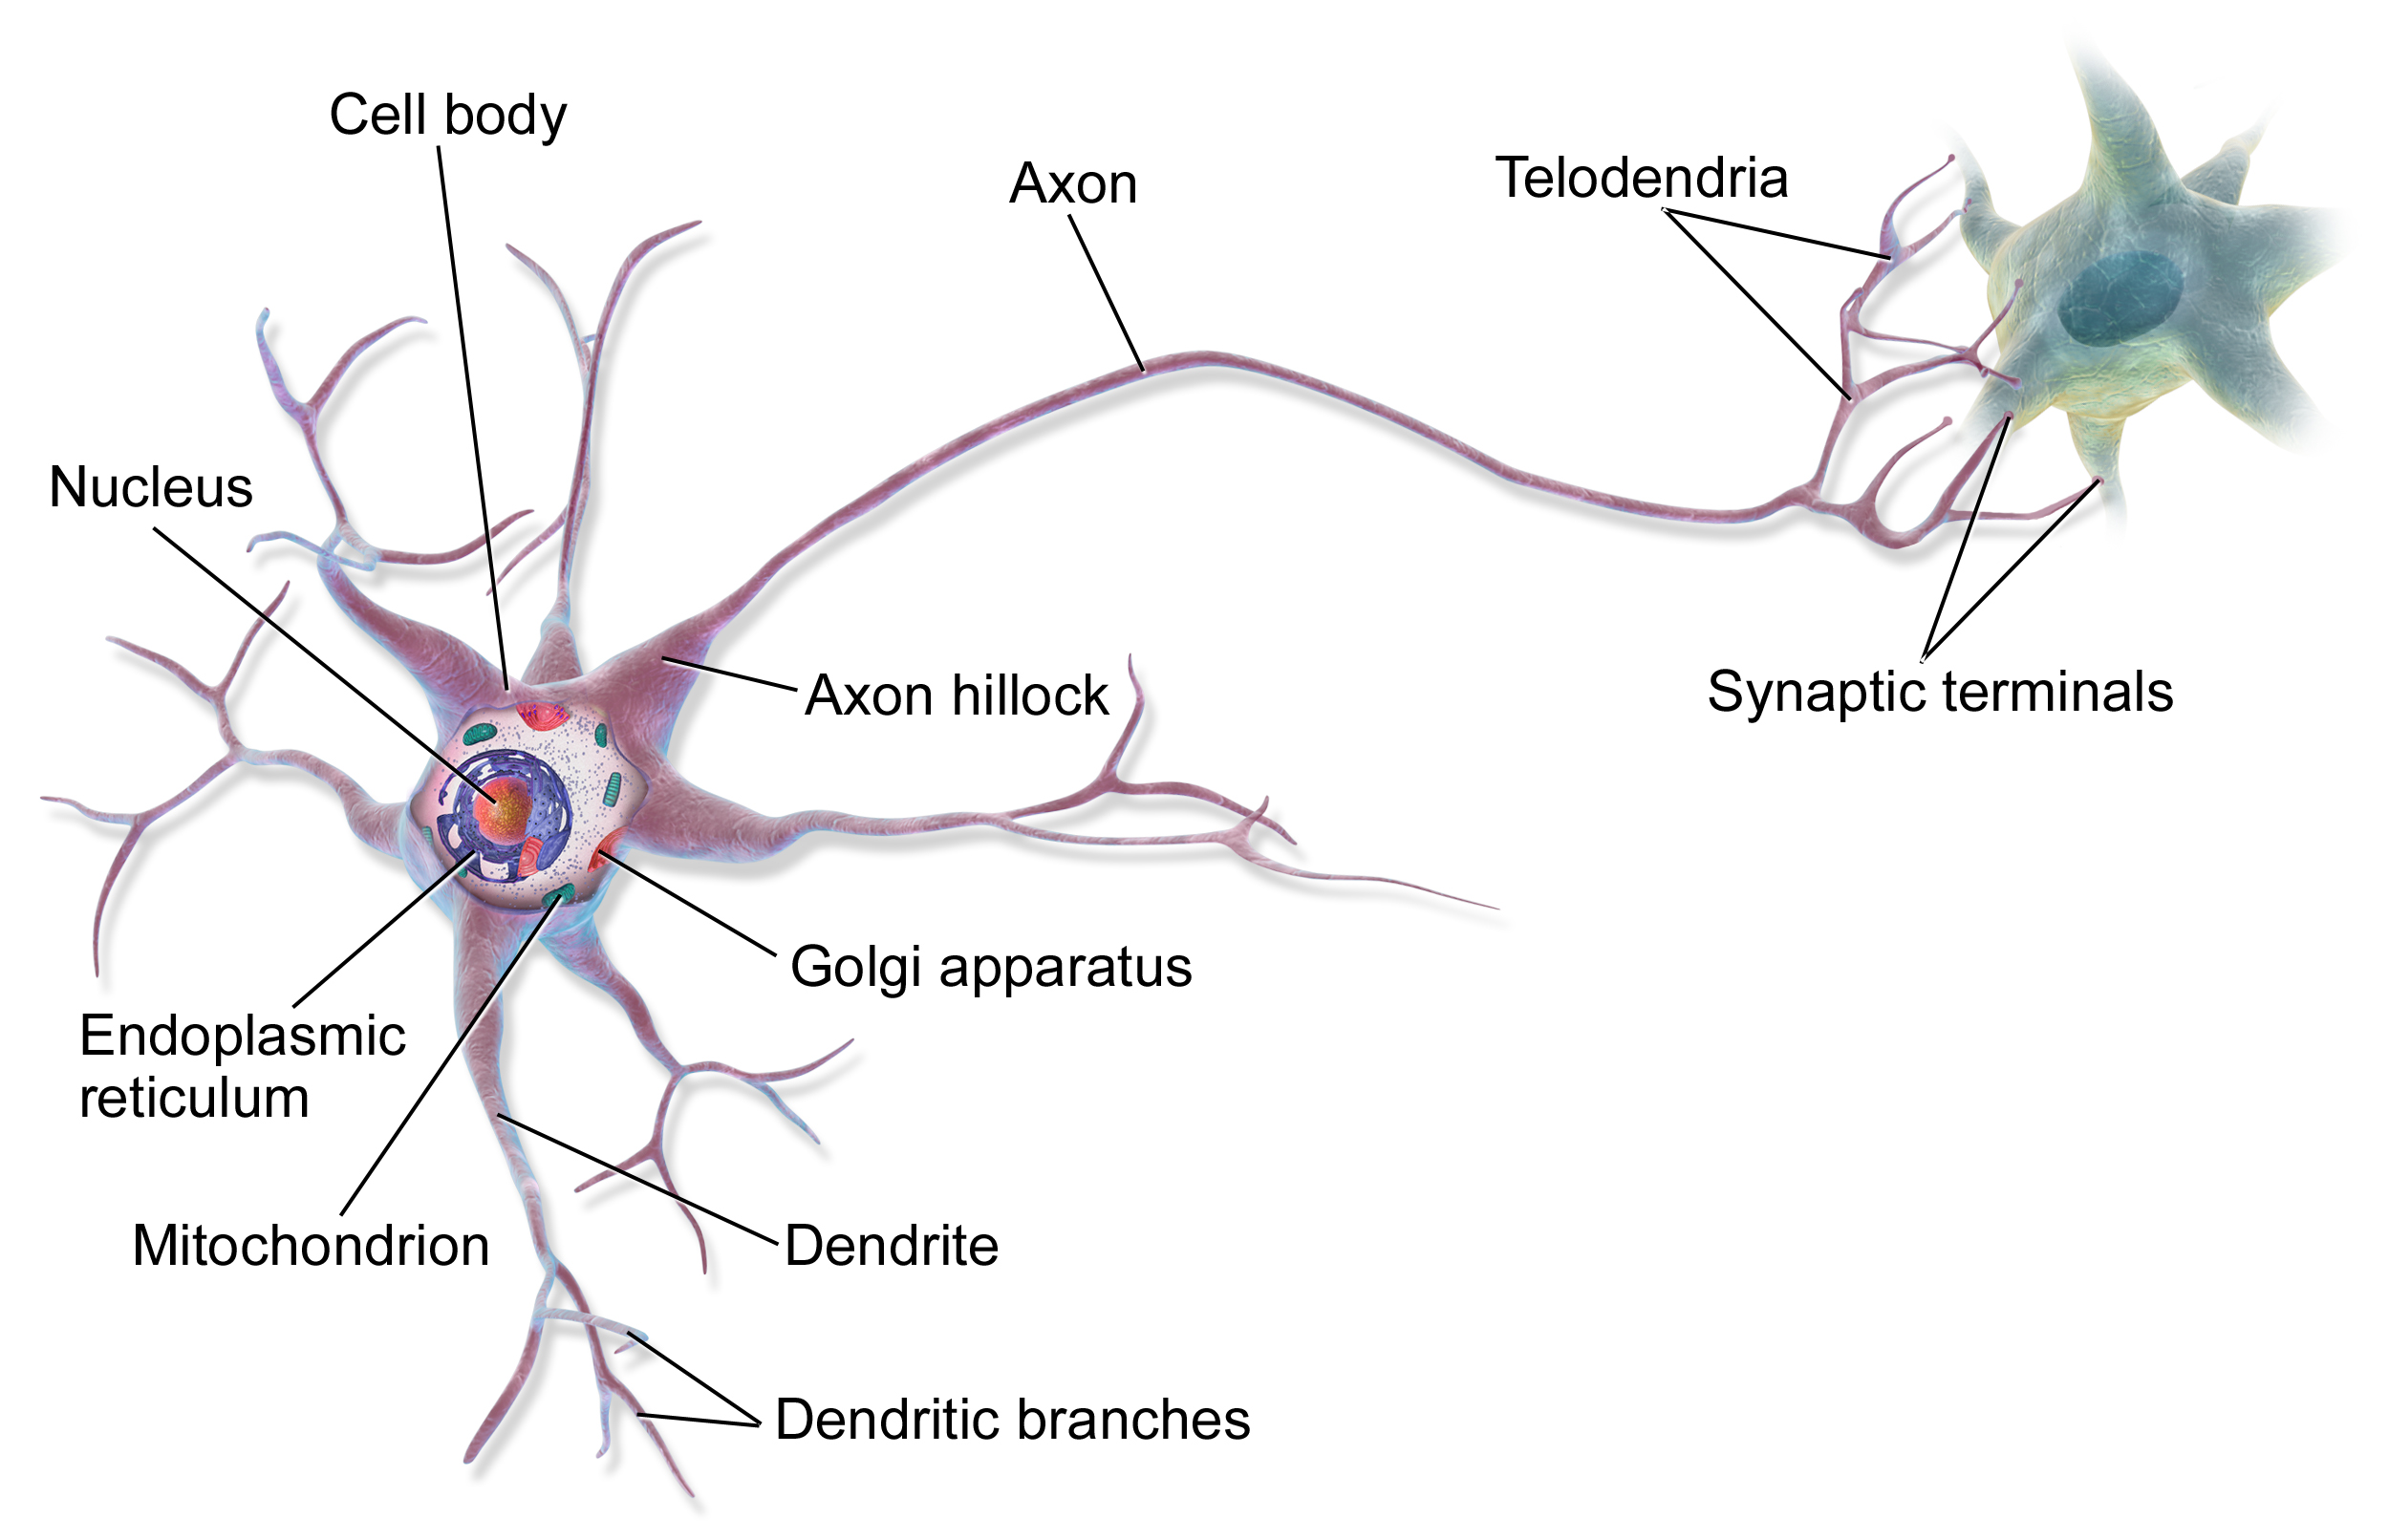
\includegraphics[clip, width=0.75\columnwidth]{figures/deeplearning/neuron.png}
  \end{center}
  
  %\vspace*{-6pt}
  \caption[Biological Neuron]{Biological Neuron\footnotemark}
  \label{fig:biological_neuron}
  %\vspace*{-12pt}
\end{figure}

\footnotetext{Image created by Bruce Blaus, released under Creative Commons under \url{https://commons.wikimedia.org/wiki/File:Blausen_0657_MultipolarNeuron.png}}

Before we look at the first artificial neuron, let us first take a look at its biological counterpart for which we included a sketch in Figure \ref{fig:biological_neuron}. Since the neuron is a specialized cell, it contains a cell body with a nucleus. Around its core, the neuron branches out into \textit{dendrites}. These dendrites can be seen as the inputs of the neuron. The output of the neuron is a single, long dendrite, called the \textit{axon}. The axon can have extremely different length, ranging from less than a millimeter up to meters. At its end, the axon branches out into \textit{telondendrias}, which end in \textit{synapic terminals} (also called \textit{synapses}). The synapses themselves are connected to the dendrites of other neurons or muscles. If the neuron receives a signal through its dendrites and the signal strength rises up to a certain level, the neuron answers by sending short electrical impulses called \textit{action potentials} (APs) down its axon. These APs result in neurotransmitters being released in the synapses - transmitting the signal to the next cell. Neurotransmitters are chemical substances which means, the electrical (digital) signal gets converted into an analog signal at the synapses. This signal at the synapses can lead to a further transmission of signals or inhibit the next neuron from firing. 

While a single biological neuron is fairly simple, neurons form extremely complicated structures. The human brain consists of around 86 billion neurons which work as a unit and form a lot of specialized substructures to control our body, process images from our eyes, or acoustic signals from our ears. Even more impressive is the fact, that these structures are not static and most of these capabilities can be learned and thus are flexible. Even though we do not understand all these processes in biological neurons in detail, we can try to use artificial version of these building blocks and experiment with them.

\begin{figure}[ht]
  \begin{center}
  \resizebox{0.95\columnwidth}{!}{%
  \begin{tabular}{cccc}
  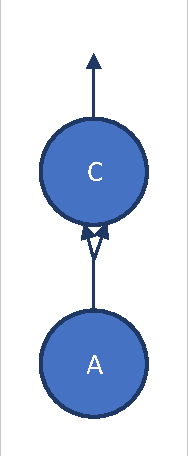
\includegraphics[clip, trim=10px 10px 10px 10px, height=5cm, page=1]{figures/deeplearning/ArtificialNeuron.pdf}  &
  \includegraphics[clip, trim=10px 10px 10px 10px, height=5cm, page=2]{figures/deeplearning/ArtificialNeuron.pdf} & 
  \includegraphics[clip, trim=10px 10px 10px 10px, height=5cm, page=3]{figures/deeplearning/ArtificialNeuron.pdf} &
  \includegraphics[clip, trim=10px 10px 10px 10px, height=5cm, page=4]{figures/deeplearning/ArtificialNeuron.pdf}\\
  {$C = A$} &
  {$C = A \wedge B$} &
  {$C = A \vee B$} &
  {$C = A \wedge \neg B$}\\
  
  \end{tabular}
  }%
  \end{center}
  %\vspace*{-12pt}
  \caption[Artificial Neurons for Logical Expressions]{Artificial neurons for logical expressions. The neurons (circles) A, B compute the output C via connections (arrows).}
  \label{fig:ArtificialNeuron}
  %\vspace*{-12pt}
\end{figure}

The first version of this artificial neuron was proposed early in 1943 by Warren McCulloch and Walter Pitts \cite{mcculloch1943logical}. They showed how logical expressions can be build with a network of binary neurons. Logical neurons activate their output if at least two of their inputs are active. Figure \ref{fig:ArtificialNeuron} shows an example for the basic logical operations \textit{and}, \textit{or} and \textit{not}. It is clear, that we can express arbitrary logical formulas in conjunctive or disjunctive normal form using these neurons. However neurons which only support binary values are not able to compute functions which is a major shortcoming. McCulloch and Pitts therefore also proposed a second version: The \textit{Threshold Logic Unit} (TLU). TLUs are able to perform continuous linear function computations. They achieve this by first computing a weighted sum of the inputs $z = w_1x_1 + w_2, x_2 + \dots + w_n, x_n = \mathbf{x}^T\mathbf{w}$ and then applying a step function. This step function sets the output to $+1$ if $z\geq0$ and otherwise to $0$. We included a graphical version which shows a single TLU in Figure \ref{fig:TLU}. The behavior of the step function matches the behavior of biological neurons, which either fire their signal at full signal strength or do not fire at all. A single TLU is able to perform binary classification tasks (output is either $1$ or $0$ depending on the class). Training the TLU then means to find the right weights for each input. The question is how to find these weights?

\begin{figure}[ht]
  
  \begin{center}
      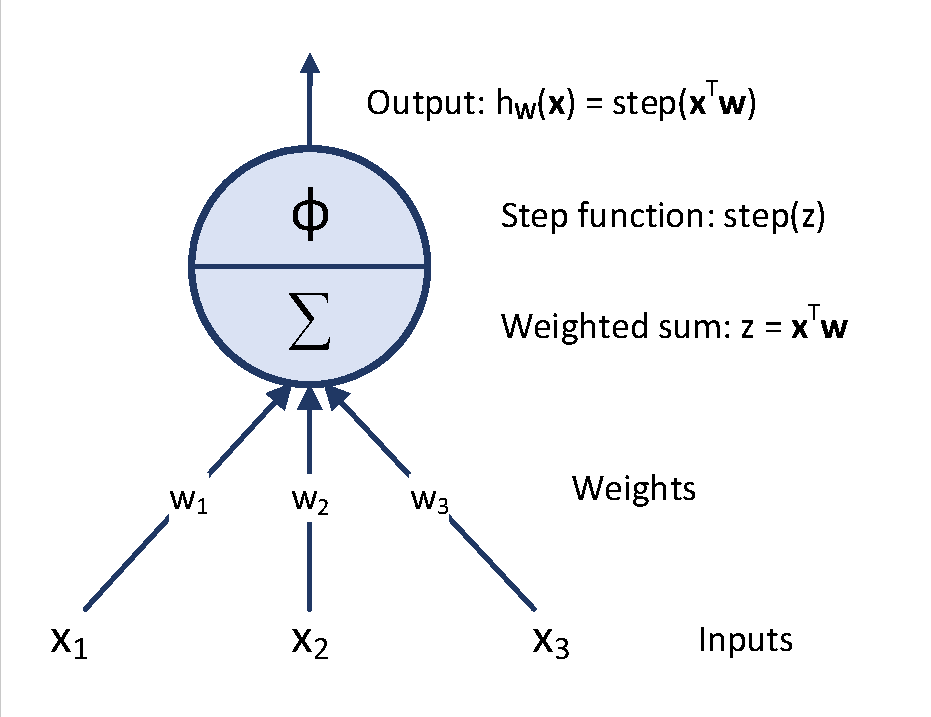
\includegraphics[trim=10px 10px 10px 10px, clip, width=0.5\columnwidth]{figures/deeplearning/TLU.pdf}
  \end{center}
  
  %\vspace*{-6pt}
  \caption[Threshold Logic Unit]{A \textit{threshold logic unit} is an artificial neuron which computes its output by a weighted sum of its inputs and a special step function.}
  \label{fig:TLU}
  %\vspace*{-12pt}
\end{figure}

 In 1957 Frank Rosenblatt invented the \textit{Perceptron} as an extension of the TLU. A perceptron is a combination of multiple TLUs to a layer of neurons, which all are connected to the inputs. We included an example in Figure \ref{fig:Perceptron}. Usually a bias neuron is added to the inputs to give the network more flexibility. The neurons in the first layer build the \textit{input layer} and just pass the input signal to the neurons in the \textit{output layer}. Both layers are \textit{fully connected} meaning every neuron in the input layer is connected to every neuron in the output layer. The output of the output layers TLUs can be computed at once by 

 \[h_{\mathbf{W}, \mathbf{b}}(\mathbf{X}) = \phi(\mathbf{XW} + \mathbf{b})\]

where $\mathbf{X}$ represents the input, $\mathbf{W}$ is a concatenation of all the weights of the TLUs (except for the bias neurons) and $\mathbf{b}$ represents the bias. For now the function $\phi$ is the step function. 

\begin{figure}[ht]
  
  \begin{center}
      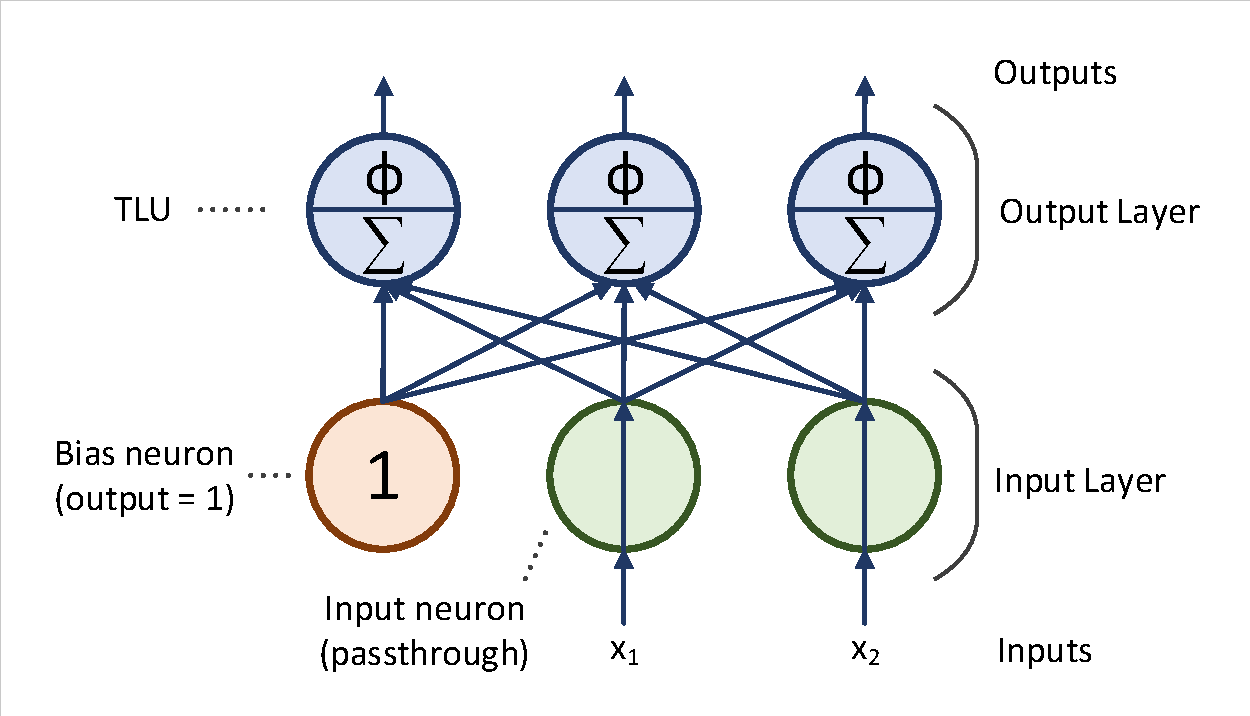
\includegraphics[trim=10px 10px 10px 10px, clip, width=0.7\columnwidth]{figures/deeplearning/Perceptron.pdf}
  \end{center}
  
  %\vspace*{-6pt}
  \caption[Perceptron Example]{Example for a \textit{perceptron} with 2 neurons and a bias in the input layer and 3 neurons in the output layer.}
  \label{fig:Perceptron}
  %\vspace*{-12pt}
\end{figure}

Rosenblatt also proposed a simple algorithm which is able to compute the weights for all TLUs for a given classification problem based on the error the network made. This algorithm is based on the perceptron learning rule 

\[w_{i, j}^{new} = w_{i, j} + \eta(y_j - \hat{y}_j) x_i\]

After the network classified the examples $x_i$, it updates the weights depending on the outcome - $y_j$ is the current output of the $j$th neuron and $\hat{y}_j$ the target value. The weights $w_{i, j}$ describe the weights between the $i$th input neuron and the $j$th output neuron. The parameter $\eta$ is the \textit{learning rate} for the network. The perceptron originally was build as a pure hardware implementation. The machine was connected to a camera and was one of the first machines which was able to learn weights for image recognition. \\
In 1969 it was proven by Marvin Minsky and Seymour Papert, that perceptrons are only able to compute linear functions and cannot compute a logical XOR from their inputs. Therefore perceptrons can only be used for simple linear classification tasks. However if the data is linearly separable, perceptrons are proven to converge.

\subsection{Multi-Layer Perceptrons} \label{ssec:MLPs}
So how do we actually learn nonlinear separation with TLUs if perceptrons are unable to do so? A simple but powerful extension to the original idea was to just stack multiple perceptrons on top of each other as shown in Figure \ref{fig:MLP}. 

\begin{figure}[ht]
  
  \begin{center}
      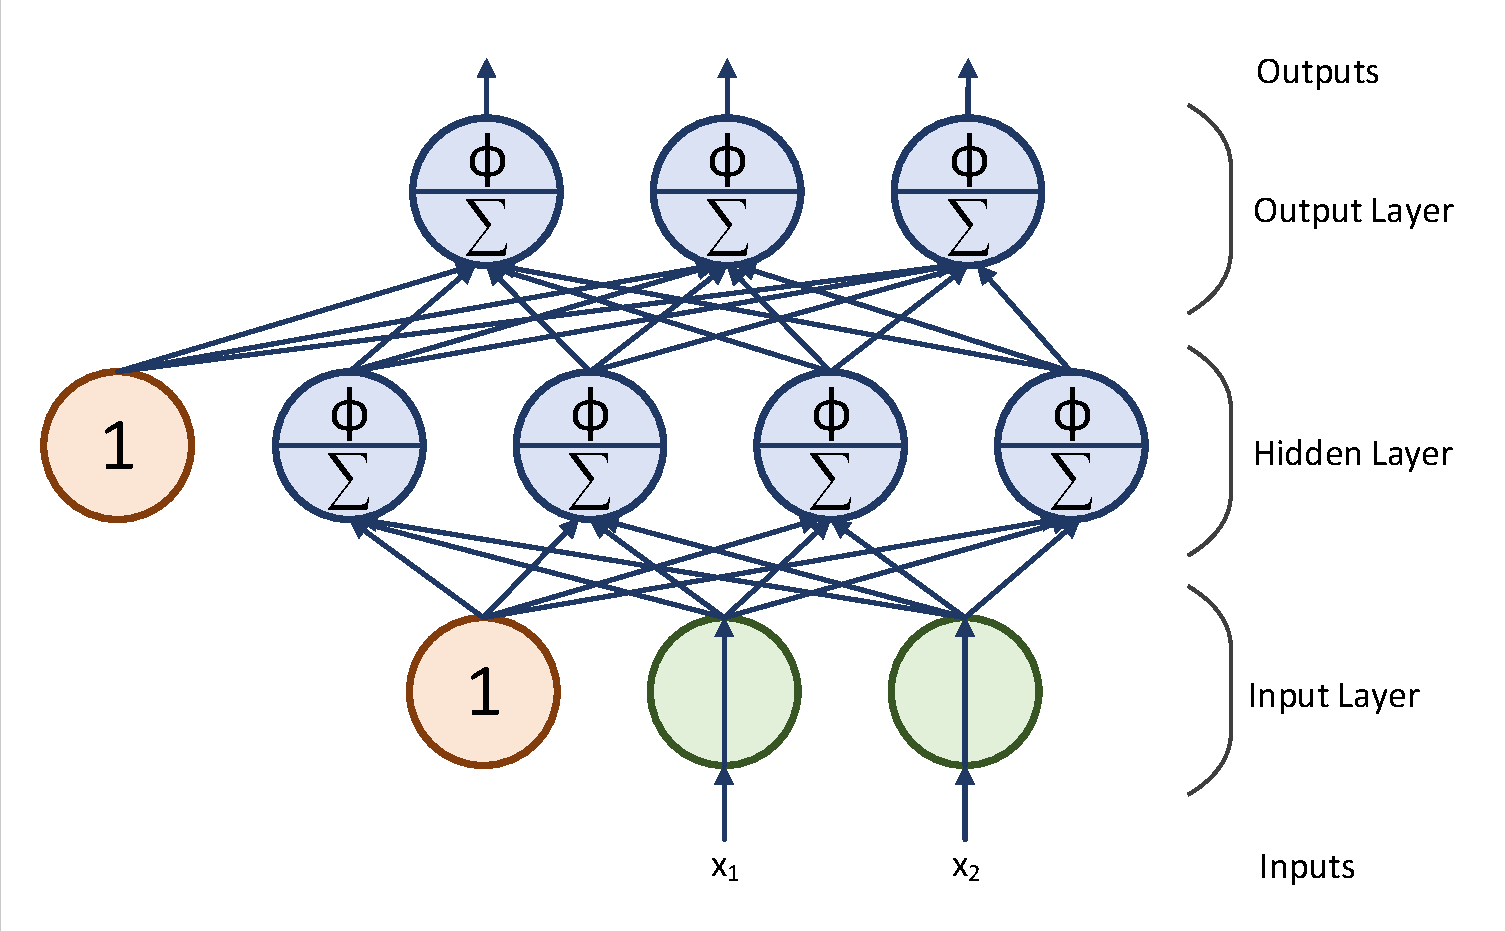
\includegraphics[trim=10px 10px 10px 10px, clip, width=0.8\columnwidth]{figures/deeplearning/MLP.pdf}
  \end{center}
  
  %\vspace*{-6pt}
  \caption[Multi-Layer Perceptron Example]{Example for a \textit{multi-layer perceptron} network with 2 neurons and a bias in the input layer and 4 neurons and a bias in the hidden layer and 3 neurons the output layer. The number of hidden layers and neurons per layer in a network can be arbitrary large.}
  \label{fig:MLP}
  %\vspace*{-12pt}
\end{figure}

This extended network actually allows to compute the XOR operation. Layers between the input and the output layer are called \textit{hidden layers} since they have no connection to the outside world. Computations are done layerwise similar to perceptrons by computing $h_{\mathbf{W}, \mathbf{b}}(\mathbf{X}) = \phi(\mathbf{XW} + \mathbf{b})$ for each layer, where $\mathbf{X}$ is the output of the previous layer. Each layer may have an individual number of neurons. The name deep learning rises from the idea of stacking more and more layers on top of each other to build \textit{deep neural networks} (DNNs). Because the input "flows" directly from the input to the output through each layer, these networks are also called \textit{Feedforward Neural Network} (FNN). The idea of stacking multiple perceptrons on top of each other was known for quite some time, but the problem was that it has been unclear how these networks could be trained. The simple perceptron algorithm does not work anymore, cause we now need to compute the error with respect to every layer. Additionally even though stacked perceptrons are able to compute XOR operations they are still limited to learning linear functions, since they are only a combination of other linear functions.

\subsection{Gradient Descent and Backpropagation} \label{sec:Backpropagation}
It took a few years, until in 1985 Rumelhart et al. were able to develop an algorithm to train multilayer networks while simultaneously introducing nonlinearity \cite{rumelhart1985learning}. Their algorithm combines the idea of \textit{gradient descent} with a method called \textit{backpropagation} which allows to calculate gradients for the weights of each layer of the network.

\begin{figure}[ht]
  
  \begin{center}
      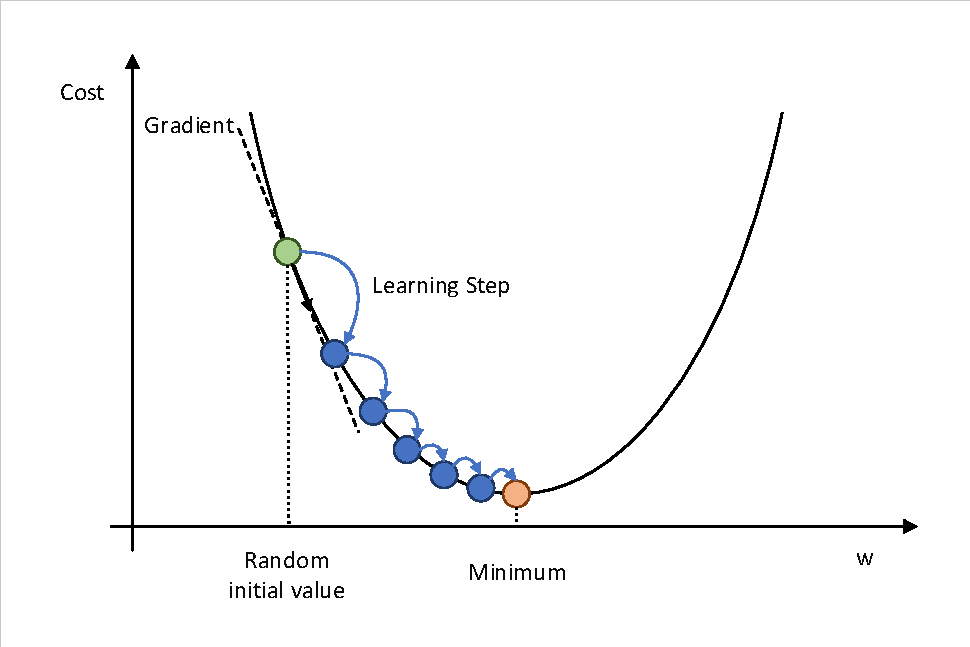
\includegraphics[trim=10px 10px 10px 10px, clip, width=0.75\columnwidth]{figures/deeplearning/GradientDescent.pdf}
  \end{center}
  
  %\vspace*{-6pt}
  \caption[Gradient Descent]{The idea of gradient descent.}
  \label{fig:GradientDescent}
  %\vspace*{-12pt}
\end{figure}

\paragraph{Gradient Descent.} Let us first look the gradient descent. Gradient descent is a method to calculate the minimum of a function. Given an arbitrary starting point on the function, gradient descent will iteratively find a series of new points leading towards a minimum (see Figure \ref{fig:GradientDescent}). Suppose we are at some point $x_k$ on our function $f$, we can then calculate the next step using the gradient $\nabla f$ of our function. We therefore can calculate 

\begin{align*}
  \delta_k &= -D_k \nabla f(x_k) \\
  \text{and } x_{k+1} &= x_k + \eta_k \delta_k
\end{align*}

as the next point closer to the minimum. The parameter $\eta$ is known as step size and in the context of deep learning is referred to as \textit{learning rate}. Usually at each step we are interested to calculate the steepest descent at the current point, since this will lead us quickly to our minimum, therefore we set $D_k = I$, with $I$ being the identity matrix. Note that there exist other approaches for second order optimization which use Hessians for $D_k$ instead.

The choice of an appropriate $\eta$ is crucial for gradient descent. Too large values will lead to points which oscillating around the minimum or even completely diverge from it, while too small values for $\eta$ might need many iterations to converge. Gradient descent also does not guarantee convergence to a global minimum and smaller learning rates increase the danger of getting stuck in a local minimum.

We now know what gradient descent does, but the question is which function can we minimize in the context of machine learning and how do we train a model by doing so? If we look at a neural network, it outputs a vector $\mathbf{z}$ at its output layer. This output is usually desired to give us some information (e.g. class probabilities in a classification task). When training we know the true output vector $\mathbf{y}$ the network should produce for some given input. Therefore we can calculate the error of the network in terms of a cost function over the dataset. Depending on the task there are several different cost functions which can be used. One of the most common ones is the \textit{mean squared error} (MSE):

\begin{equation*}
  MSE(\mathbf{x}, \theta) = \frac{1}{n} \sum^n_{i=1} (z_i - y_i)^2
\end{equation*}

Since the output vector $\mathbf{z}$ is dependent on the input vector $\mathbf{x}$ and the network weights $\theta$, but we only have control over $\theta$, we often write $MSE(\mathbf{x}, \theta)$ as $MSE(\theta)$ for short. When performing gradient descent we then calculate the gradient with respect to $\theta$. 

When implementing gradient descent for neural networks, we are sometimes interested in optimizing for multiple objectives at once. We therefore usually perform gradient decent with respect to a so-called loss function $\mathcal{L}(\theta)$ (which is equal to our cost function at the moment). We then denote the gradient of that function with respect to the network weights as $\nabla_\theta \mathcal{L}(\theta)$. A single gradient descent step for our network is then given by

\begin{equation*}
  \theta^{new} = \theta - \alpha \nabla_\theta \mathcal{L}(\theta)
\end{equation*}

Because the calculations for the gradient descent step are costly, it is usually considered sufficient to only calculate the gradient for a single sample from the dataset in each step (as opposed to calculating the gradient as a mean over the whole dataset). This procedure is called \textit{stochastic gradient descent} (SGD) and is a stochastic approximation of gradient descent. Training with SGD is less stable, but much faster. To stabilize training, SGD often uses \textit{minibatches} of data, where the gradient is calculated over a smaller batch of samples instead with a single sample.

\paragraph{Backpropagation.} Now that we know how we can calculate updates for the neural network, we need to know how it is possible to update the weights for each individual layer. This is where the \textit{backpropagation algorithm} comes in place. It mainly consists out of two phases: A forward pass, which allows us to determine the error (e.g. using MSE) and a backwards pass which determines which layer was involved to which extend with the error.

Let us look at the phases in more detail. The forward pass takes a sample (or a batch of samples) and propagates them through the network. For each layer, we collect the output activations and store them for later. After passing the input through the network and the calculation of the final output, we calculate our error like before. 

In second phase we begin at the output layer and propagate the error backwards layer by layer. This is done by calculating the weight change $\Delta w_{i, j}$ from neuron $i$ from the previous layer to neuron $j$ from the current layer by:

\begin{align*}
  \Delta w_{i, j} &= -\eta \delta_j o_i \\
  \text{with } \delta_j &= \begin{cases}
    \varphi'(v_i)(o_j - y_j) & \text{if $j$ is in the output layer}  \\
    \varphi'(v_i) \sum_k \delta_k w_{j,k} & \text{if $j$ is in a hidden layer}
  \end{cases}
\end{align*}

where the subscript always defines the number of the neuron in the layer. If the subscript is an $i$ we reference the previous layer (closer to the inputs) and $j$ references the current layer. We denote $v$ as the the pre-activation output, $o$ as the final post-activation output and $y$ as the desired output of a neuron.
When using minibatch SGD steps the weight changes are accumulated in the backpropagation step and then applied all at once. Since SGD is very sensitive to the learning rate, the parameter needs to be tuned carefully.

\subsection{Activation Functions} \label{ssec:ActivationFunctions}
When we look at the backpropagation algorithm we can see, that we need a differentiable activation function to perform error backpropagation. Also the first derivate of the activation function must be nonzero, otherwise all our gradients would always be zero. In order to use SGD the step function needs to be replaced with another activation function. Replacing the step function with a nonlinear function also resolves another problem of the original stacked perceptron, since it introduces nonlinearity into the network. This change finally allows the MLP to compute arbitrary functions and makes it the powerful tool it is today. Figure \ref{fig:ActivationFunctions} shows an overview over frequently used activation functions. Let us quickly briefly about each of them.


\begin{figure}[h!]
  \begin{center}
  \resizebox{0.9\columnwidth}{!}{%
  \begin{tabular}{cc}
  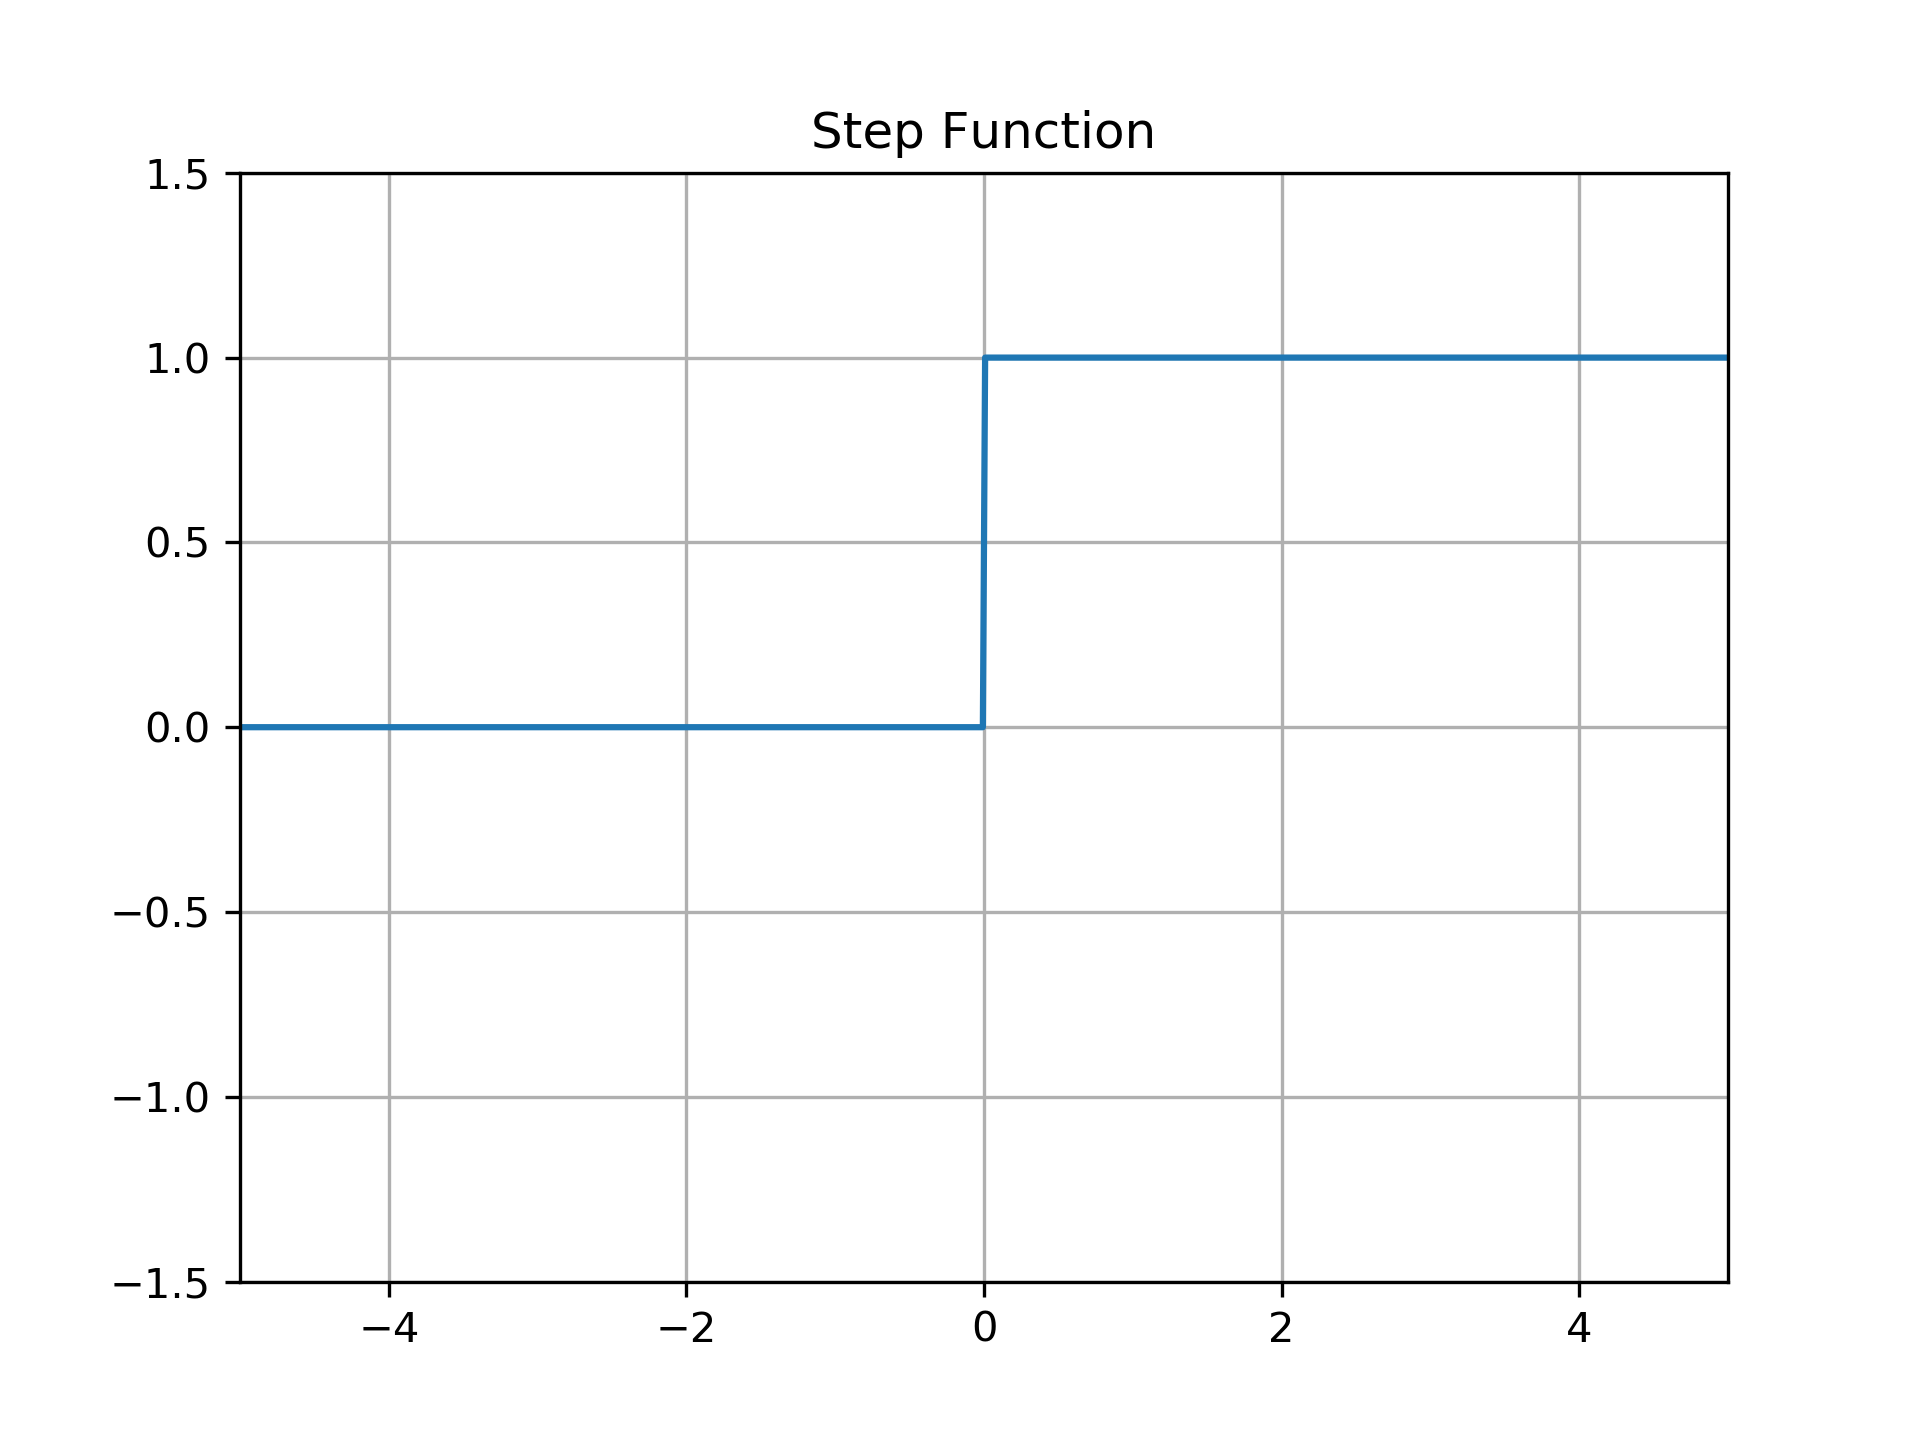
\includegraphics[clip, height=5cm]{figures/deeplearning/af_Step.png}  &
  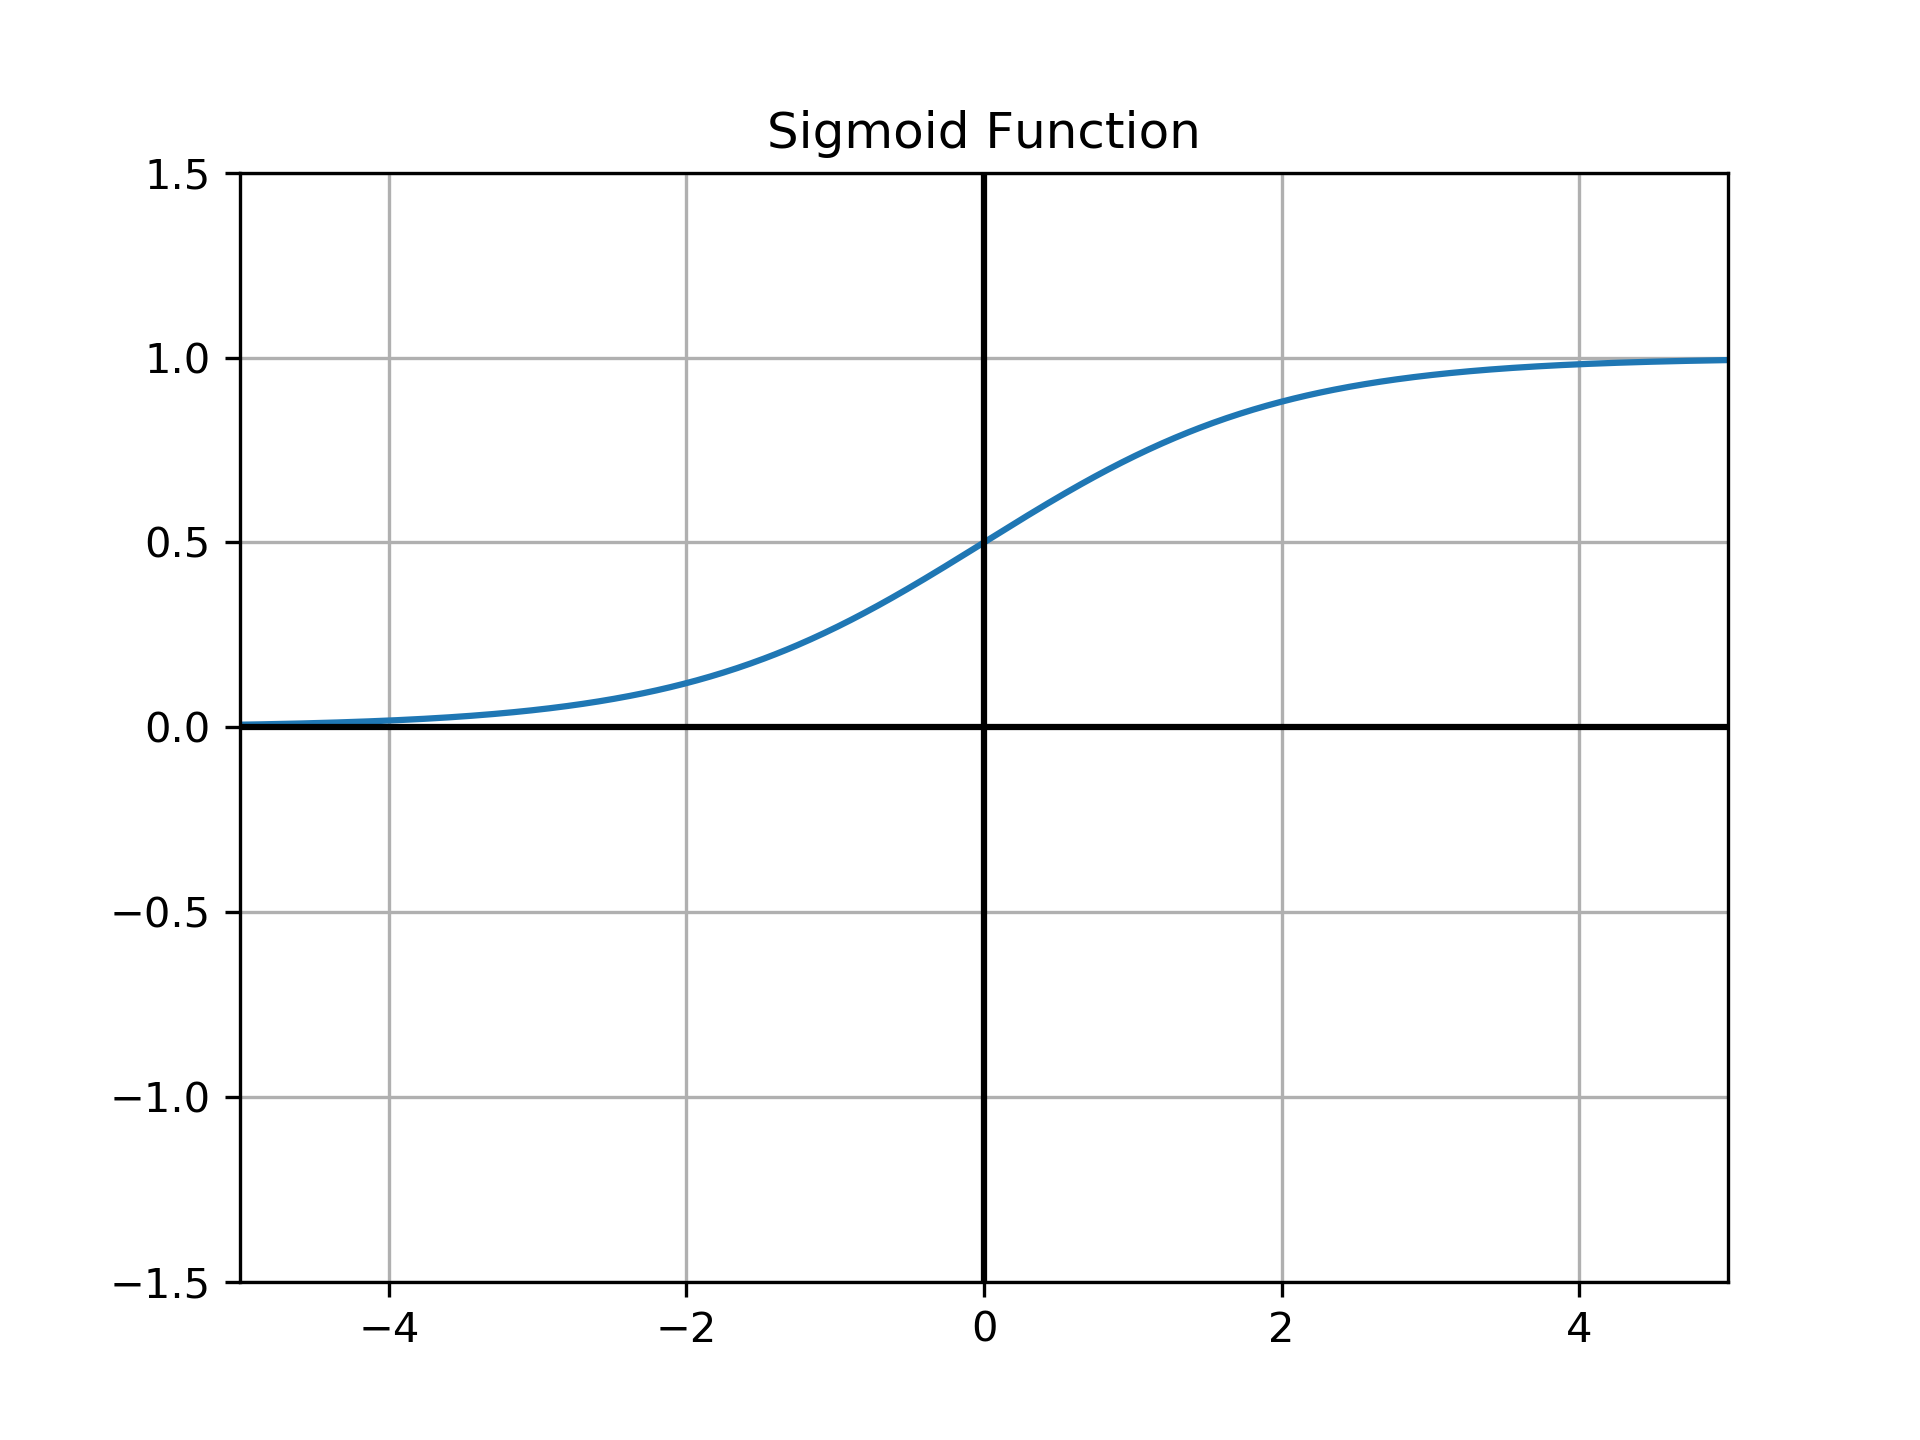
\includegraphics[clip, height=5cm]{figures/deeplearning/af_Sigmoid.png} \\
  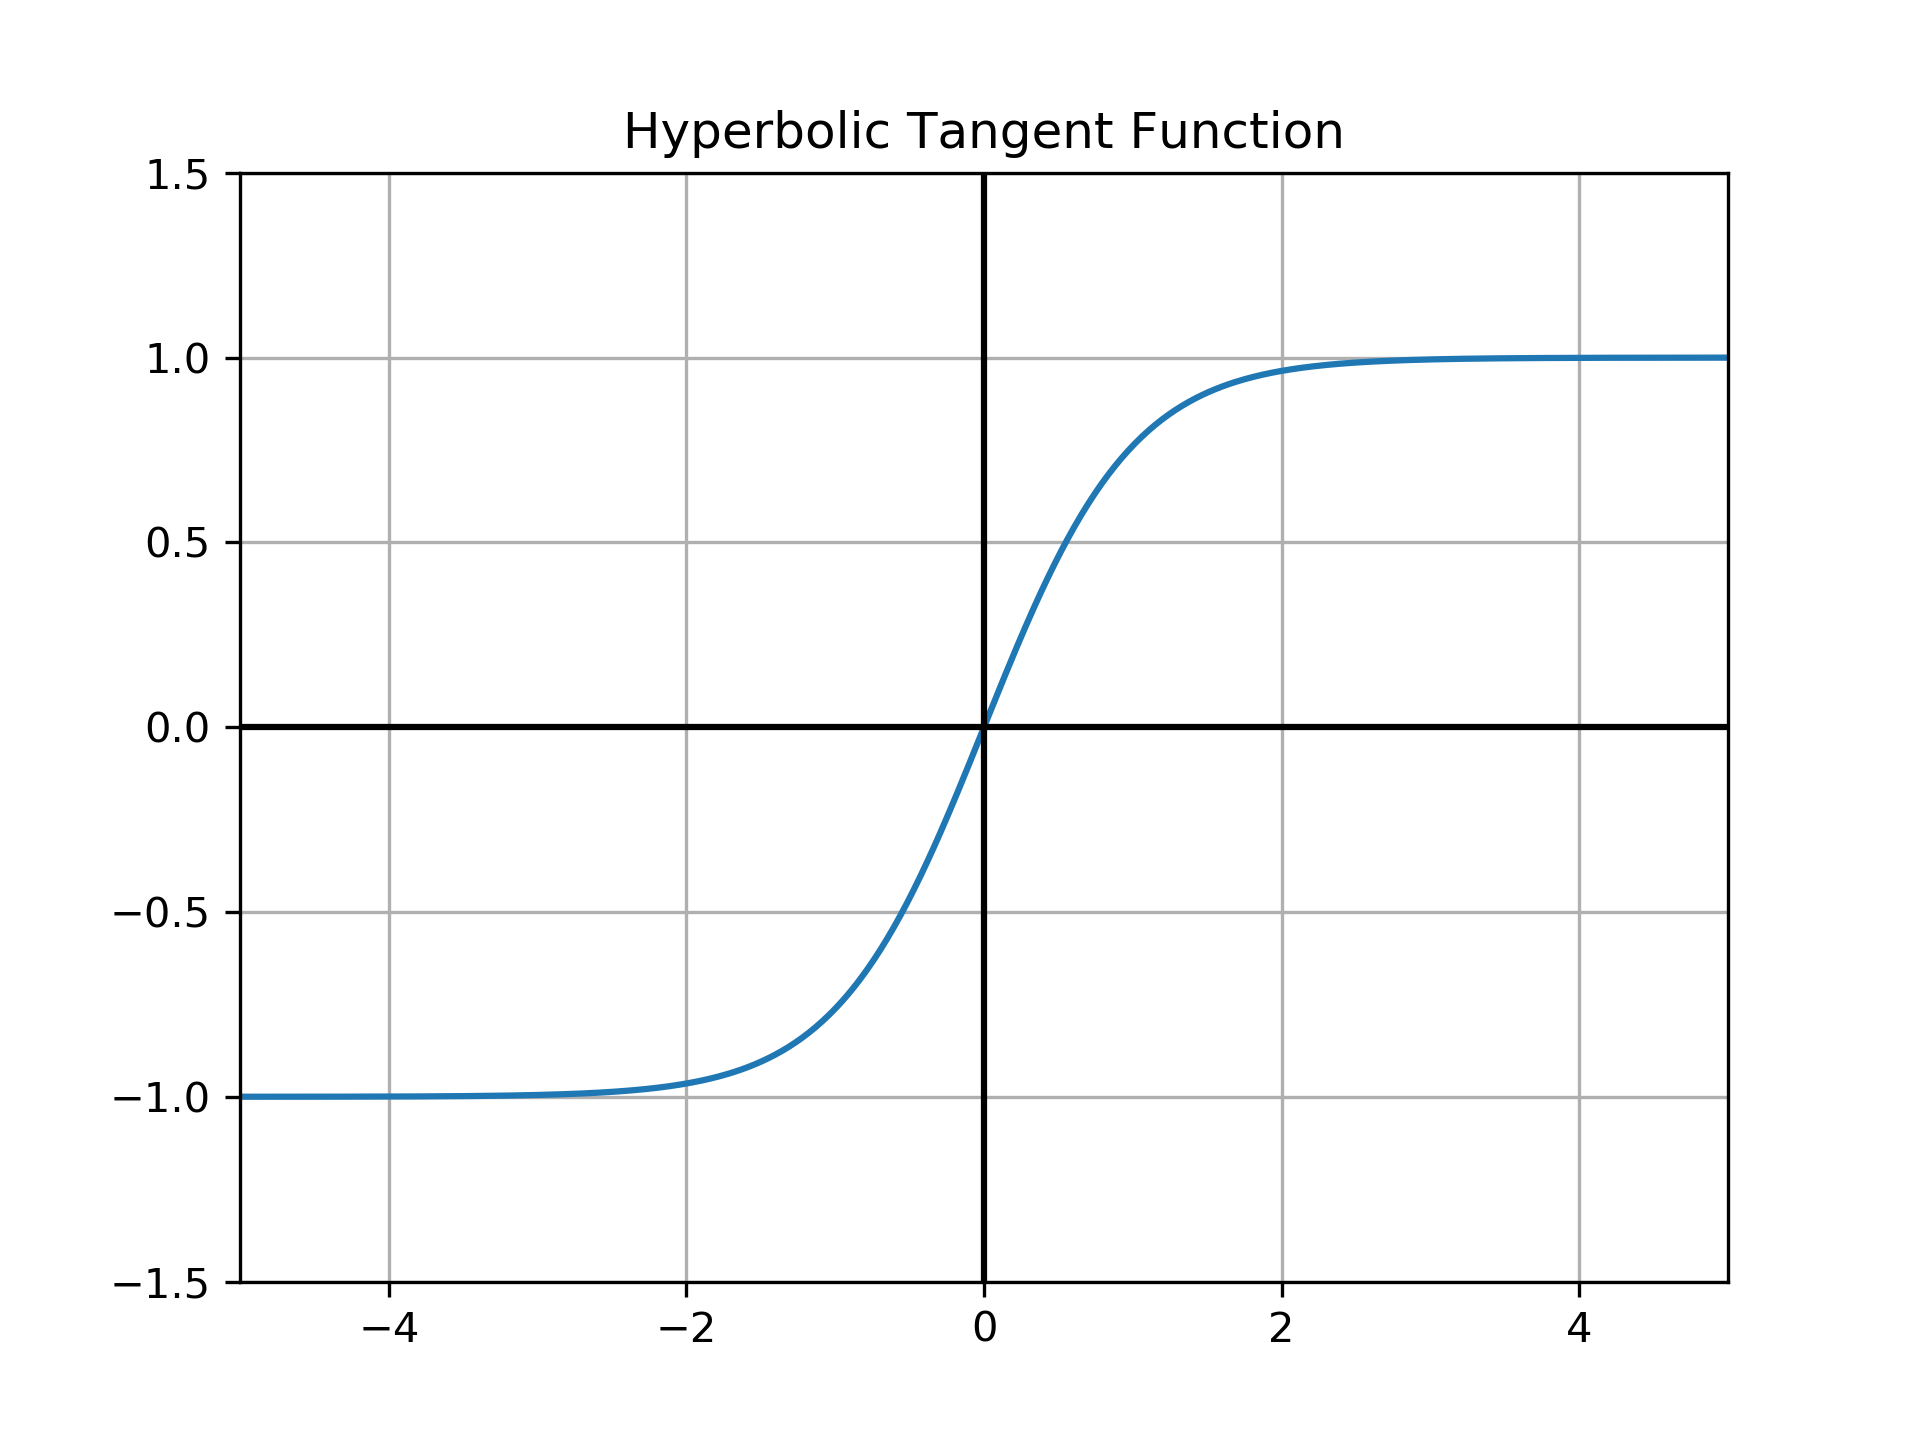
\includegraphics[clip, height=5cm]{figures/deeplearning/af_Hyperbolic.png} &
  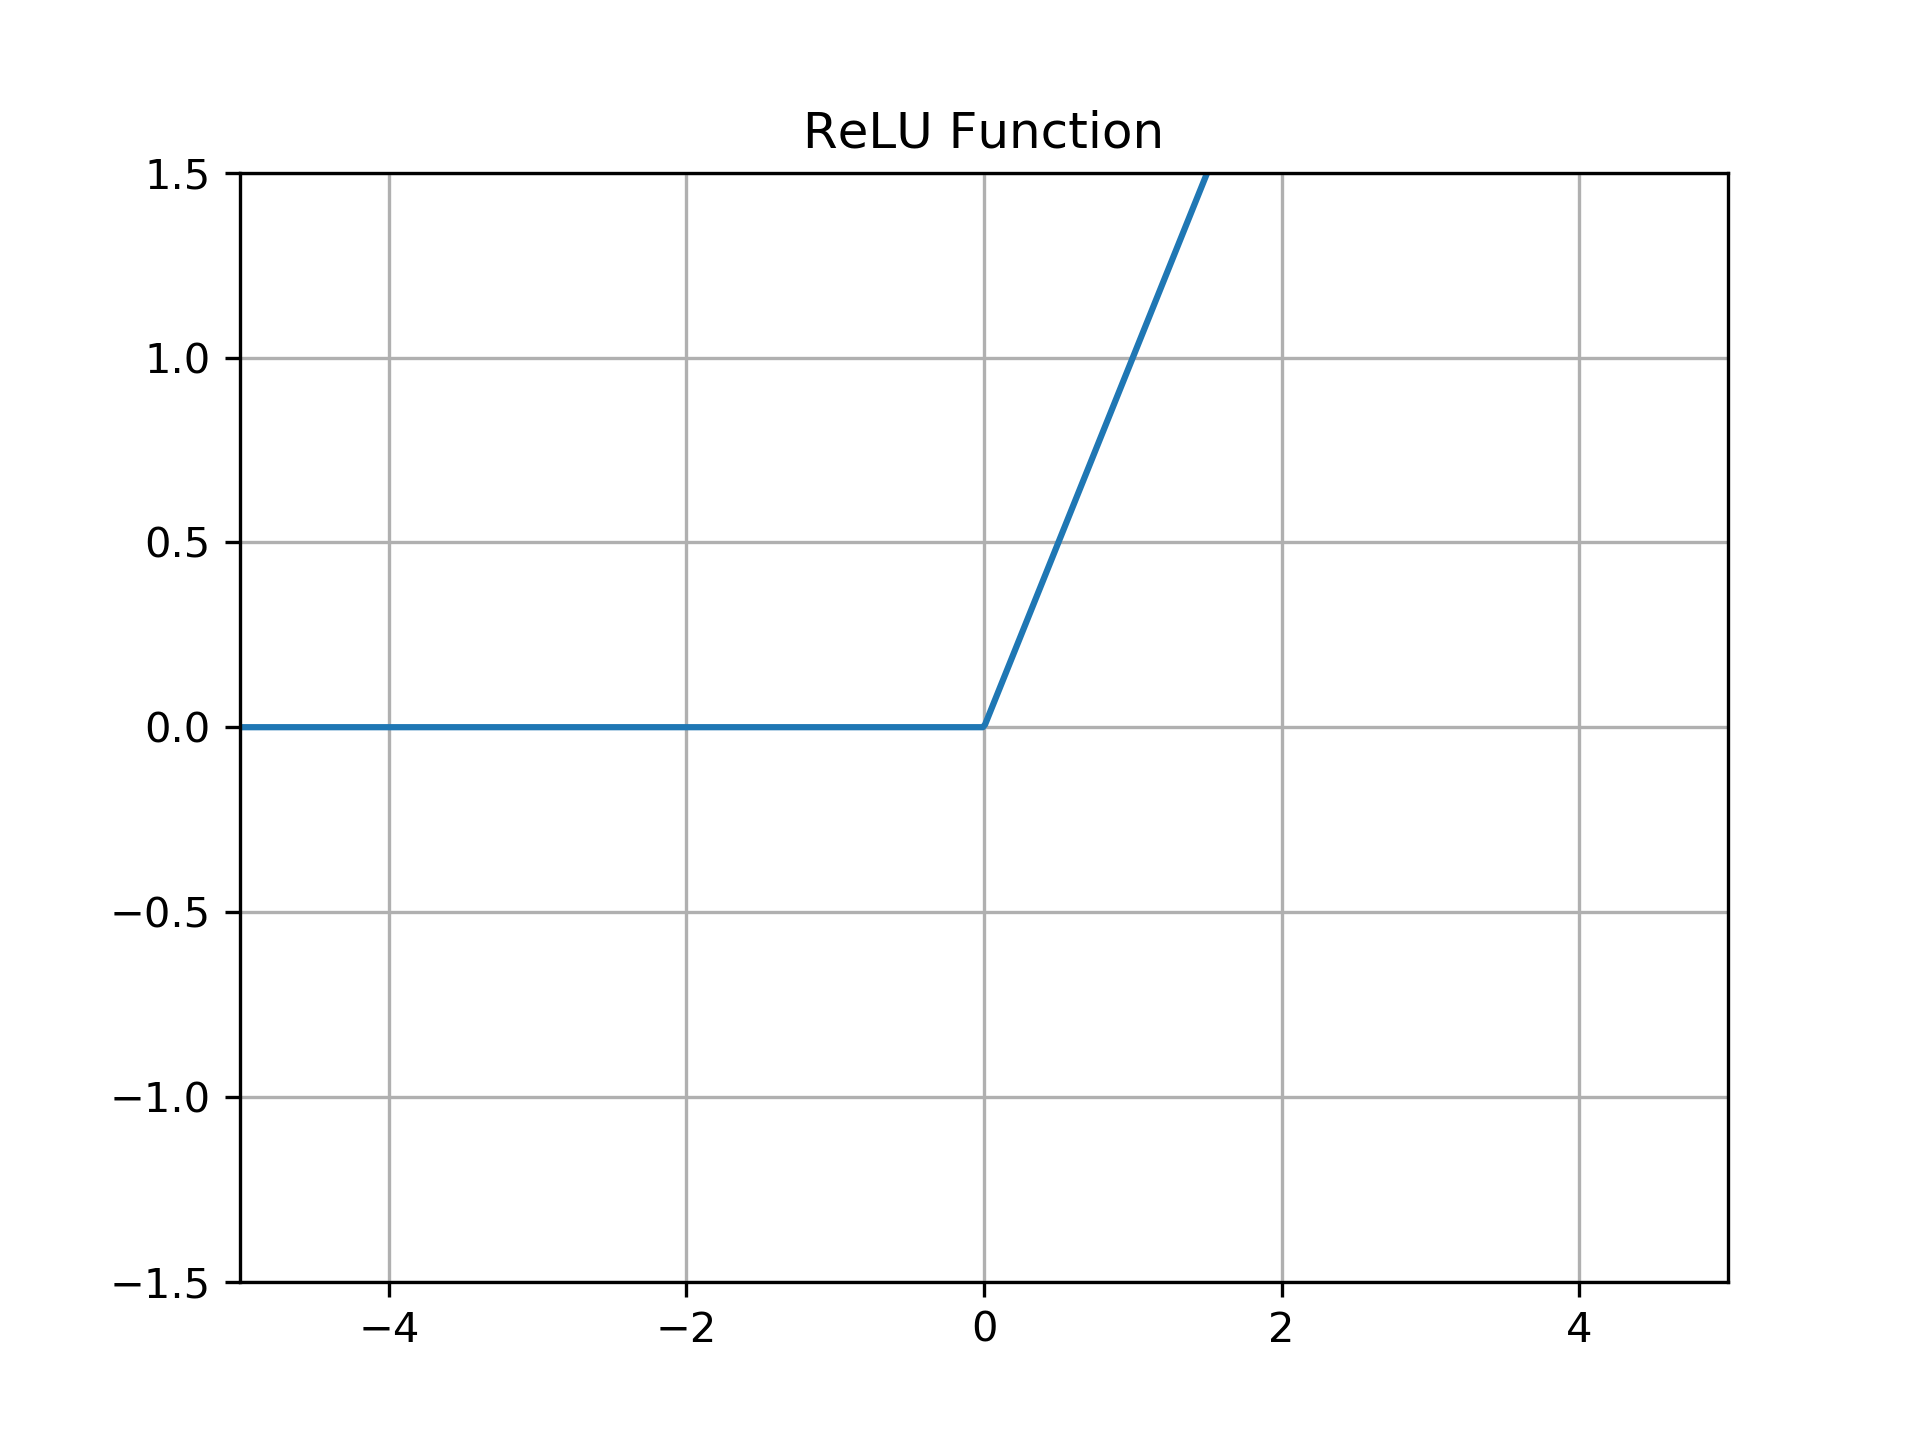
\includegraphics[clip, height=5cm]{figures/deeplearning/af_ReLU.png}  \\
  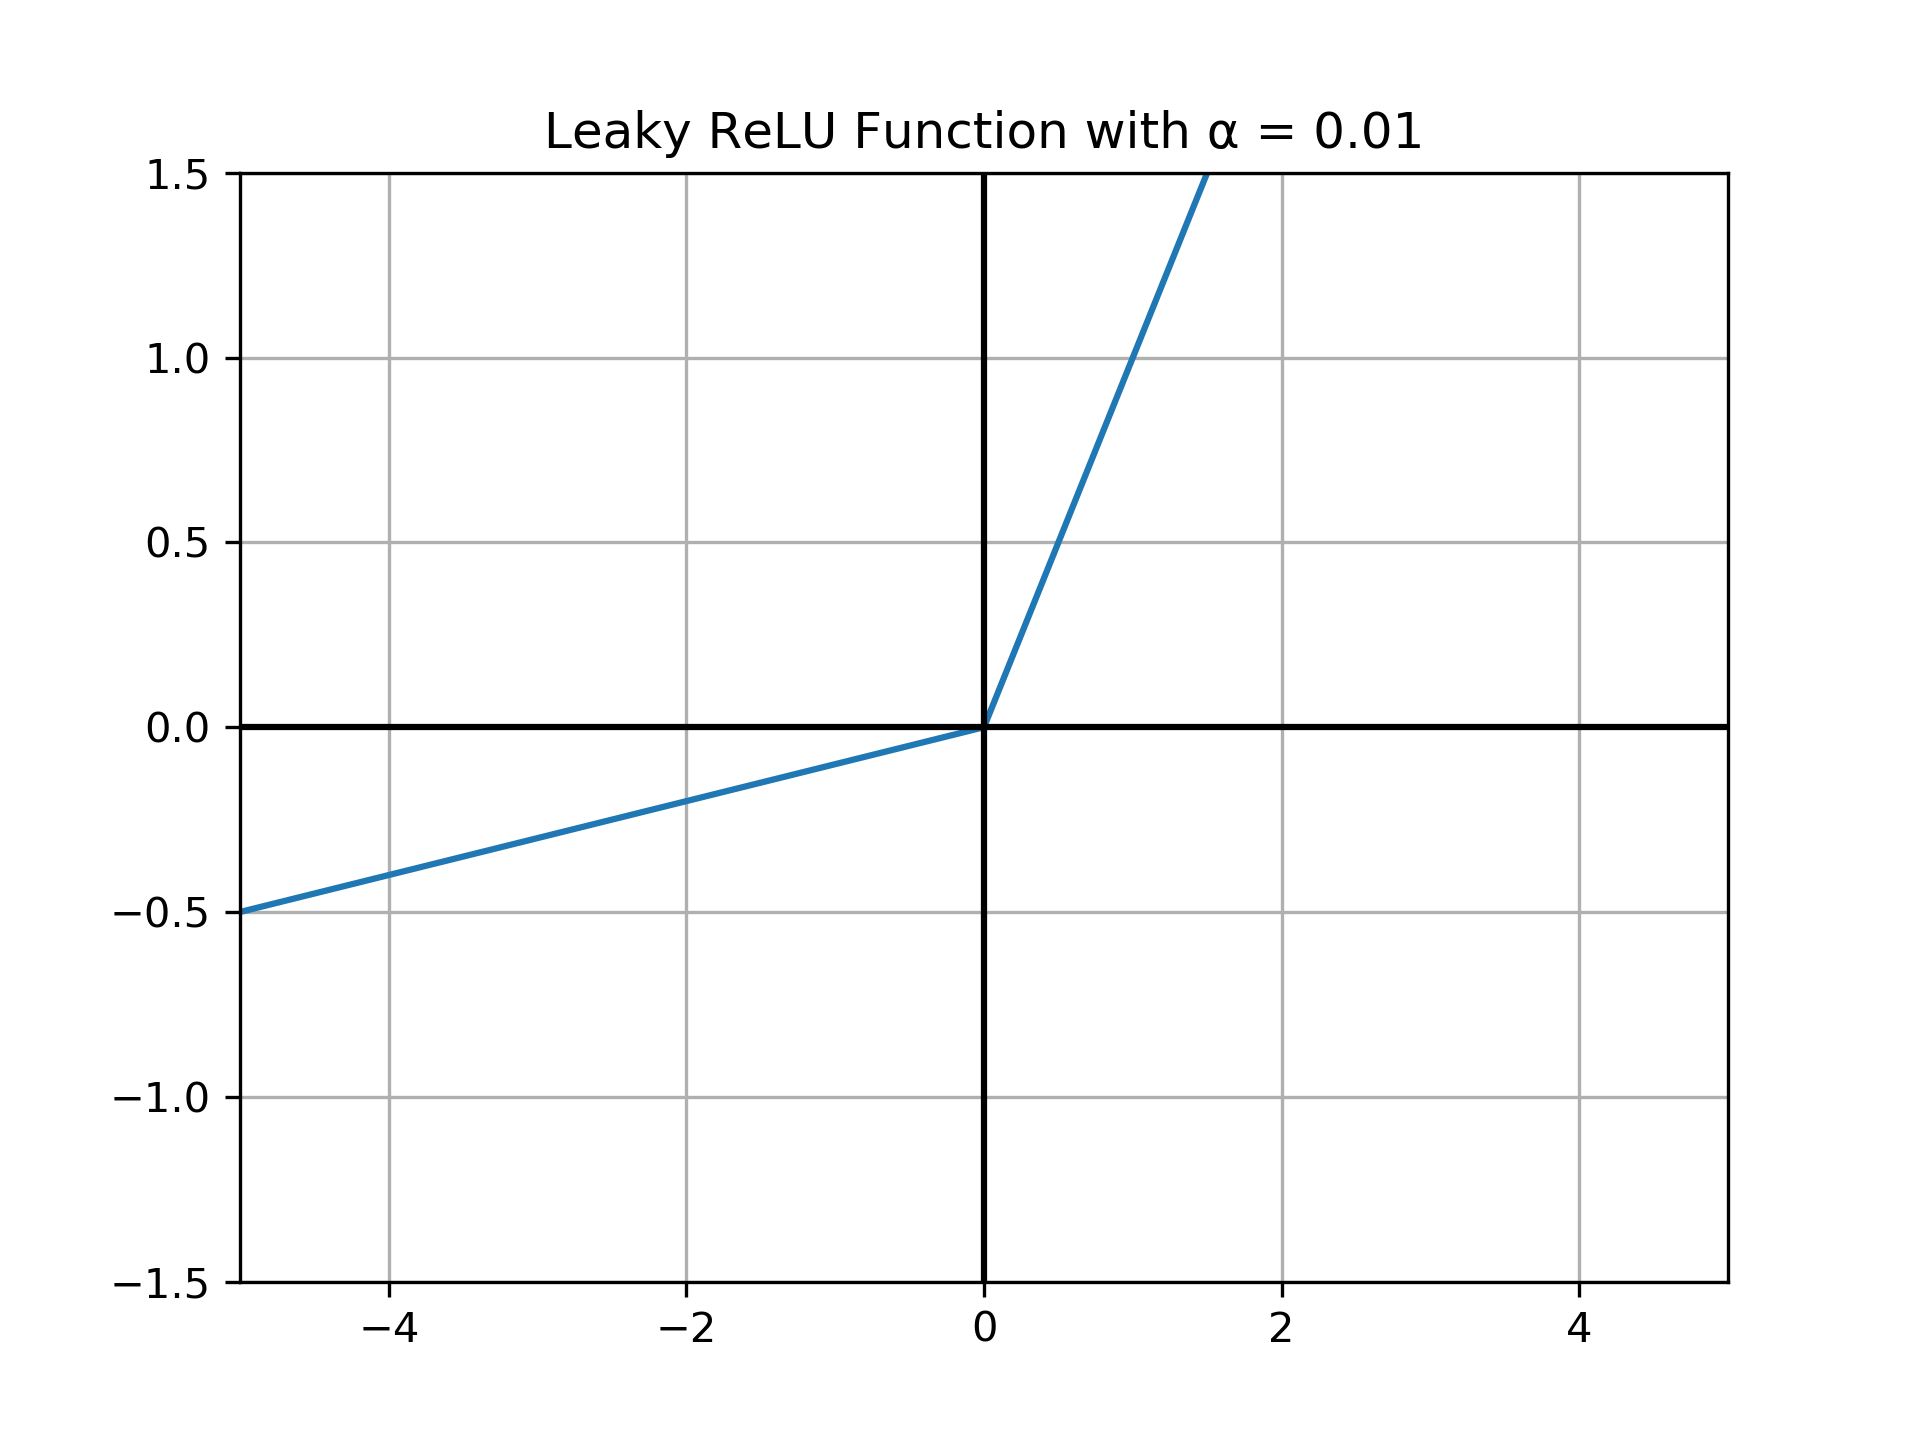
\includegraphics[clip, height=5cm]{figures/deeplearning/af_LeakyReLU.png} & 
  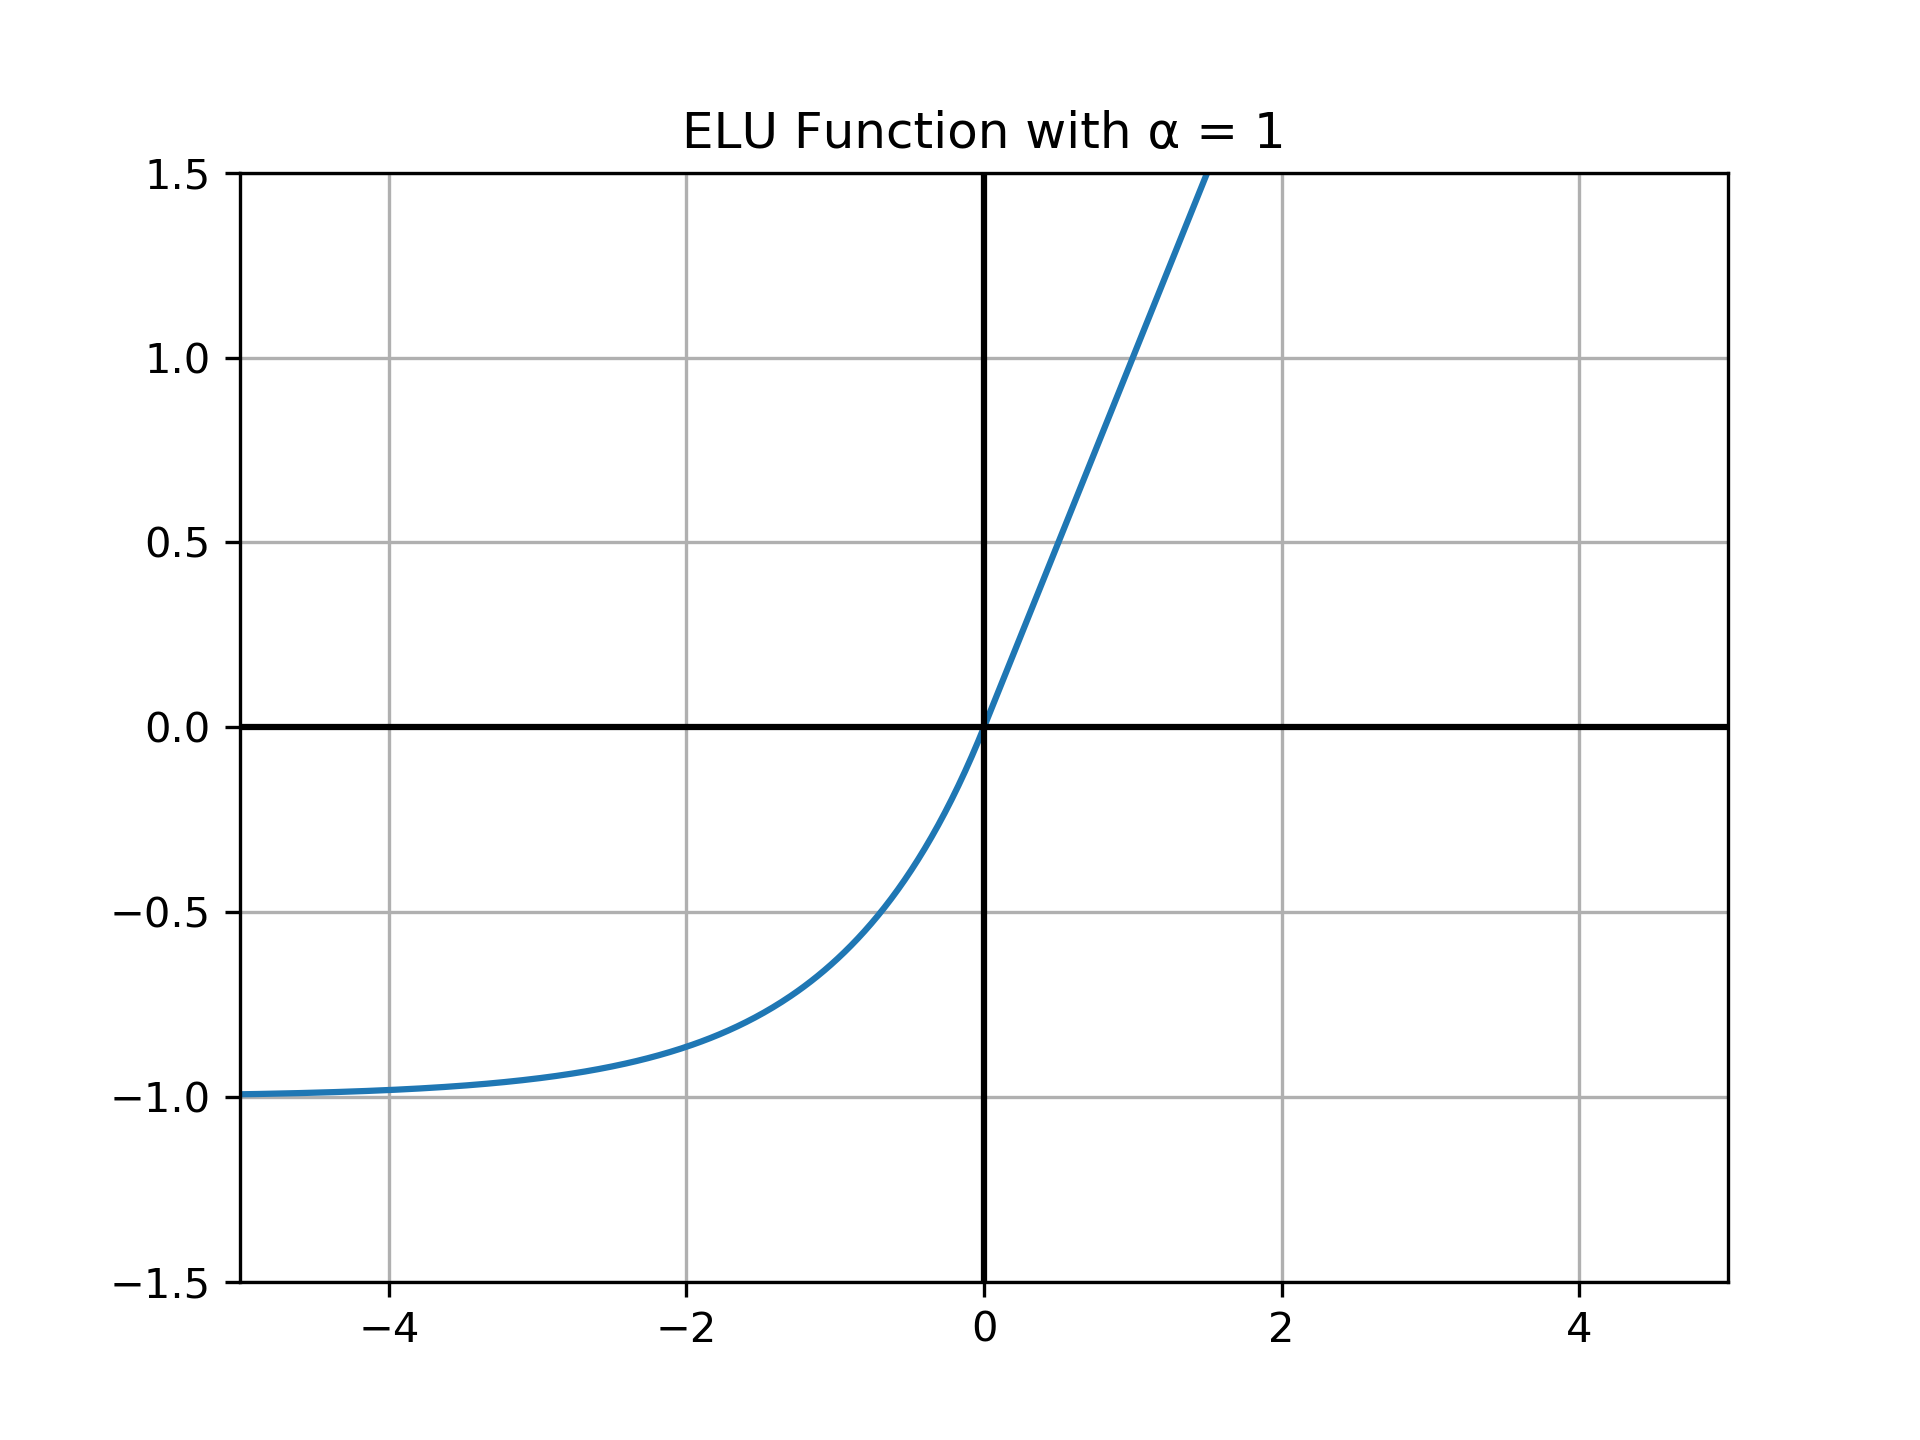
\includegraphics[clip, height=5cm]{figures/deeplearning/af_ELU.png} \\
  
  \end{tabular}
  }%
  \end{center}
  %\vspace*{-12pt}
  \caption[Activation Functions]{Common activation functions. The step function is the only function which cannot be used with the backpropagation algorithm.}
  \label{fig:ActivationFunctions}
  %\vspace*{-12pt}
\end{figure}

\begin{enumerate}
  \item The \textit{sigmoid function} $\sigma(z) = \frac{1}{1 + \exp(-z)}$ \\
    The sigmoid function was originally proposed as a replacement for the step function. It is S shaped and can express values between 0 and 1. It also is continuous, so it has a well-defined nonzero derivate everywhere, while being still similar to the step function in terms of output values.
  \item The \textit{hyperbolic tangent function} $tanh(z) = 2\sigma(2z) - 1$ \\
    The hyperbolic tangent function is similar to the sigmoid function, but its values range from $-1$ to $1$, so layer outputs are centered around 0 at the beginning of the training which speeds up convergence. However it was shown, that bounding the value of the activation function for large $z$ reduces convergence speed.
  \item The \textit{rectified linear unit function} $ReLU(z) = max(0, z)$ \\
    The ReLU function is not differentiable at $z=0$ and has a zero derivate for $z < 0$. Both these properties are not ideal, but the ReLU function is very fast to compute and still performs reasonably well in practice. It is also unbounded in terms of $z$ which further improves convergence. This makes the ReLU function one of the most used activation functions today.
  \item The \textit{leaky rectified linear unit function} $LeakyReLU_\alpha(z) = max(\alpha z, z)$ \\
    One problem with the ReLU function is, that when the weighted sum of the inputs of a neuron is negative for all training instances, the neuron itself will never output anything other than 0 again - the neuron essentially dies. To prevent this the leaky ReLU function has a leak which makes the derivate of the function nonzero for $z < 0$ and prevents the neuron from never learning anything again. The parameter $\alpha$ controls how large the leak should be and can also be learned at training time \cite{xu2015empirical}.
  \item The \textit{exponential linear unit function}
  
  \[ELU_\alpha = 
  \begin{cases} 
    \alpha(\exp(z) - 1) & \text{if } z < 0 \\
    z  & \text{if } z \geq 0
  \end{cases} \]

  Just like the Leaky ReLU function, the ELU function has a nonzero gradient for $z < 0$. If $\alpha = 1$ the ELU function is smooth everywhere. Therefore the ELU function performs better than the Leaky ReLU function, but it is harder to compute. \cite{clevert2015fast} There also exists an extension called SELU which stands for \textit{scaled exponential linear unit} \cite{klambauer2017self} and results in network layers which include self-normalization and therefore preserve a mean of 1 and a standard deviation of 0 during training. This further speeds up training and also showed to improve the results at test time.
  
\end{enumerate}

\subsection{Challenges} \label{sec:NNChallenges}
We saw how we can build neural networks and how they can be trained using gradient descent. Problems - like handwritten recognition - which were extremely complicated for a long time can now be solved with learned models. While in theory we now have the tools to build and train networks, in reality we would quickly encounter problems with networks which just do not learn what we want them to learn. In this Section we want to present some of the most common problems when training neural networks, while also looking at techniques used to avoid them.

\paragraph{Slow Convergence.}
While gradient descent is guaranteed to converge to some minimum if the learning rate is sufficiently small, it makes no guarantees of how much time this convergence process might need. Our simple gradient descent algorithm is only dependent on the first derivate and therefore only "looks" at the slope for the current point. This produces two major problems: If we are on a flat spot of the optimization surface, the gradients will be very small, slowing down training in an "uninteresting" area. The second problem is that always going into the direction of the steepest descent is not the fastest way to the minimum. Instead we would need to additionally look at the second derivate to determine which direction would be optimal. 

To reduce the influence of these problems, a variety of techniques were developed over the years. The basic idea is, that the learning rate does not necessarily have to be a constant, instead we change the step size for each step of gradient descent dynamically depending on the curvature of the optimization surface. For flat regions we could increase the learning rate to compensate for the smaller gradients and lower the learning rate if we detect unstable learning. Directly calculating second derivates has shown to be computationally too expensive. Instead algorithms try to make assumptions about the surface by looking at past gradients. An example of these methods is the idea of \textit{momentum}. 

The momentum method was also proposed by Rumelhart et al. in their backpropagation paper \cite{rumelhart1986learning}. The name originates from real physical momentum, where we think of a particle which is accelerated by a force in a direction. For gradient descent the idea is, that successive gradients usually point in roughly the same direction. Therefore we could improve convergence speed, by just applying the same gradient multiple times. To avoid overshooting, at each step we remember the gradient and compute the new gradient as a linear combination: 
    \[\Delta w = \eta \Delta w - \alpha \nabla f(x_k)\]

Momentum helps to reduce oscillation and is better at avoiding local minima, since the learning process now has the possibility to go over small "hills" in the optimization surface.

The momentum method can easily combined with a second idea: \textit{Learning rate schedules}. Picking an initial learning rate that is optimal for the whole learning process is hard. Initially we will be far from the optimum and need a higher learning rate to converge faster and avoid local minima and over time, the training process might get closer to the optimum but begin to oscillate around it, because the learning rate is too high. To always work with an optimal learning rate, we need to adjust it over time and these strategies are the learning schedules. Some often used schedules are:

\begin{enumerate}
  \item \textit{Linear Scheduling}. The easiest schedule is a linear schedule where the learning rate is a function of $\eta(t) = \eta_0 - (\eta_0 * t/s)$. The effective learning rate is linearly annealed from a starting learning rate $\eta_0$ to zero. The parameter $s$ is set to be the total number of training steps for SGD.
  \item \textit{Power Scheduling}. The learning rate is a function of the form $\eta(t) = \eta_0 / (1 + t/s)^c$ with the hyperparameters $c$ - the exponent - and $s$ - the number of steps. With power scheduling, the learning rate will decrease every $s$ steps, arriving at $\eta_0 / 2$ after $s$ steps, $\eta_0 / 3$ after $2s$ steps and so on. This results in an effective learning rate which quickly drops and then decreases more and more slowly over the course of training.
  \item \textit{Exponential Scheduling}. The learning rate is a function of $\eta(t) = \eta_0 \cdot 0.1^{t/s}$. The learning rate will therefore drop by a factor of 10 every $s$ steps.
  \item \textit{Performance Scheduling}. Measure the validation error every $N$ steps and reduce the learning rate by a factor $\gamma$ when the error did not drop. 
\end{enumerate}

There also exist a lot of other schedules like piecewise scheduling, where the learning rate is defined for specific parts of the training process. The choice of the learning rate schedule is dependent on the task and also influence by other factors like overfitting.

Since the learning rate is the most important hyperparameter for deep learning over the years many other more sophisticated methods were developed, most notable \textit{AdaGrad} \cite{duchi2011adaptive}, \textit{RMSProp} \cite{tieleman2012lecture} and \textit{Adam} \cite{kingma2014adam} which are usually used in nowadays neural network frameworks. All these algorithms use the past gradients to calculate per-parameter learning rates based on a given starting learning rate. They often make use of momentum optimization and can be used in conjunction with learning rate schedules.


\paragraph{Overfitting.}
\textit{Overfitting} is a recurring problem for all machine learning techniques. When training on a training dataset, we expect the trained model to have the same performance on new never seen before data. To achieve this, our goal is to learn a representation of our input data. The problem arises when the model is too closely fit to the training dataset, which often happens if our model has too many parameters and if we trained our model too long. Overfitted models often show an extremely low training error of close to 0\%, while on test time  the model performs very bad. Overfitted models usually did not learn a representation of the data, but instead just "remember" each sample from the training dataset. We therefore also speak about models which fail to generalize. An example for overfitting in a classification task is given in Figure \ref{fig:Overfitting}. We can see, that the overfitted model did not ignore the noise in the training data and instead created a decision boundary which perfectly separates both classes in the training dataset, but does not model the true distribution behind the data.

\begin{figure}[ht]
  
  \begin{center}
    \resizebox{0.95\columnwidth}{!}{%
    \begin{tabular}{ccc}
    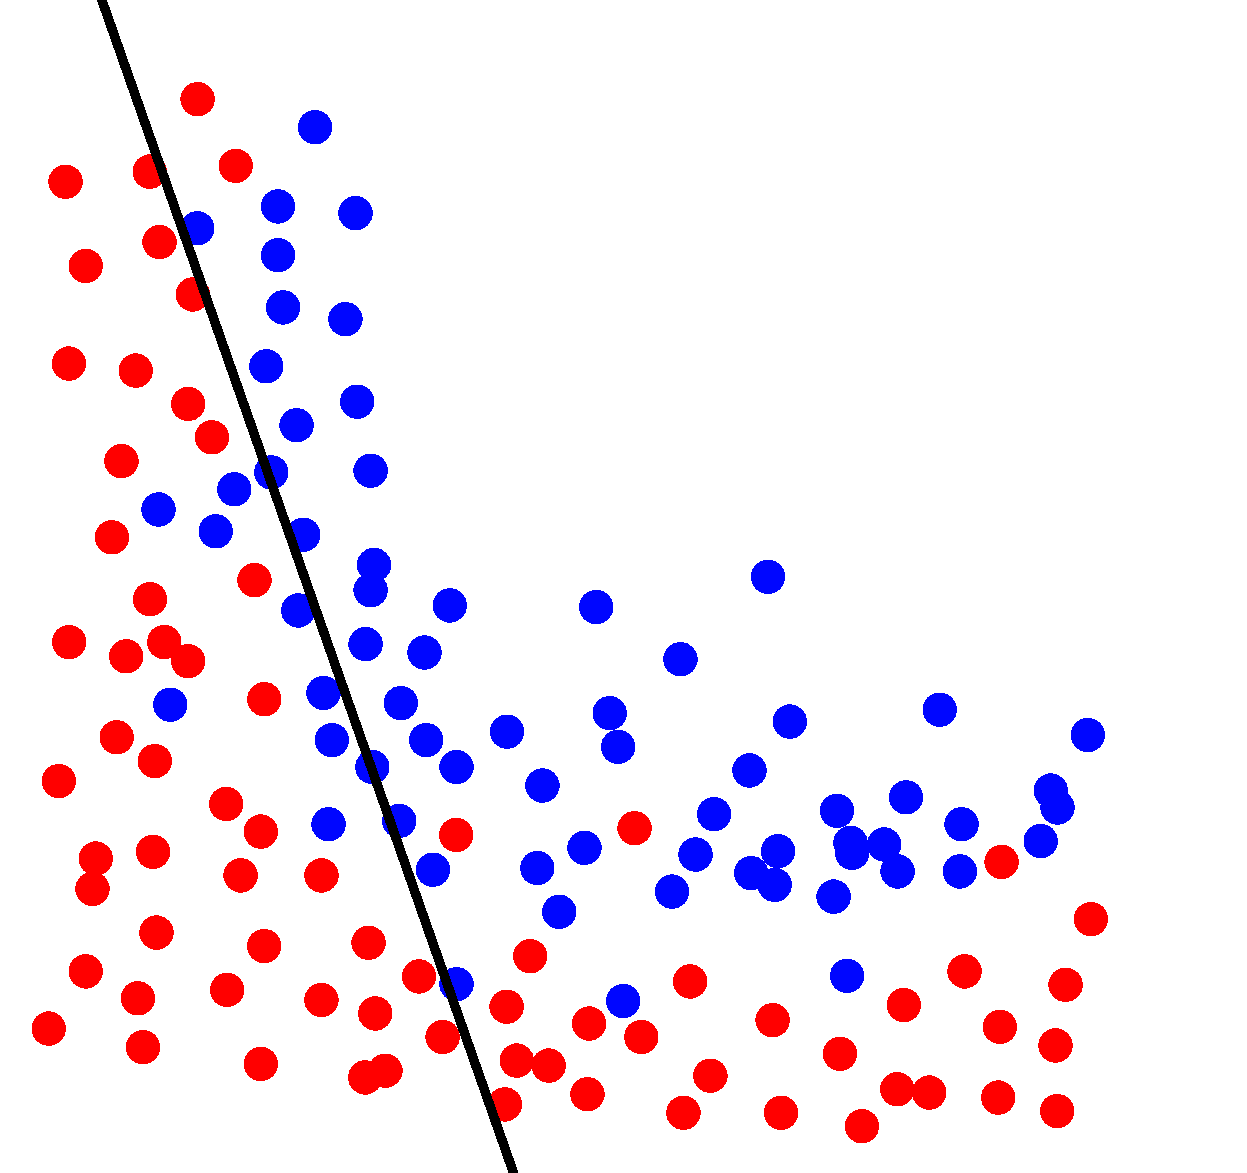
\includegraphics[clip, height=5cm]{figures/deeplearning/Underfitting.pdf}  &
    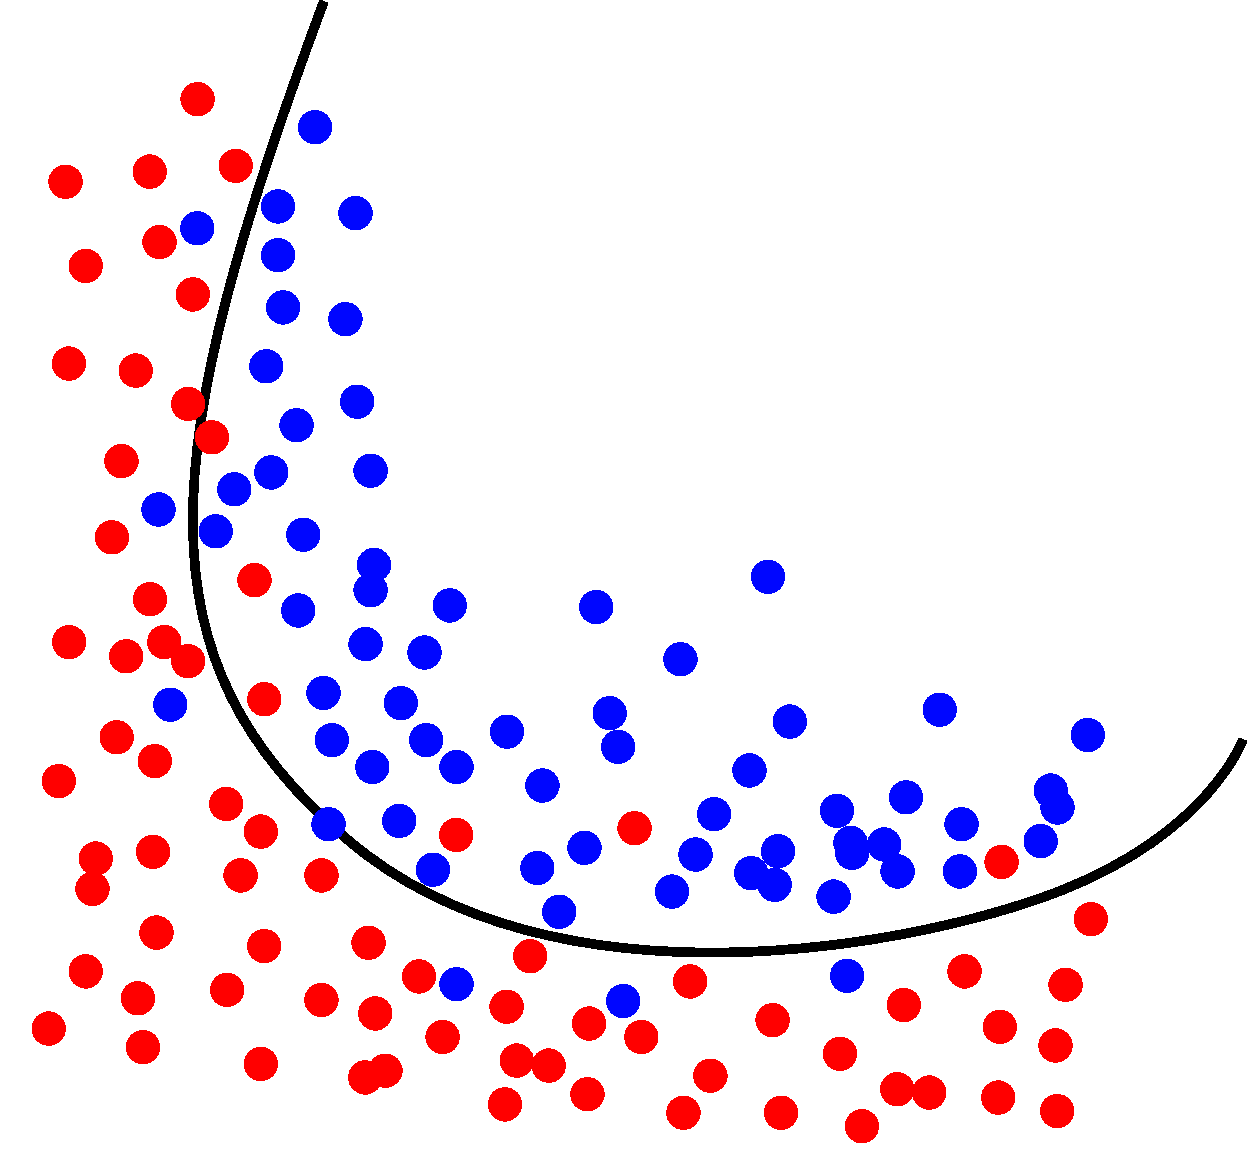
\includegraphics[clip, height=5cm]{figures/deeplearning/IdealModel.pdf} & 
    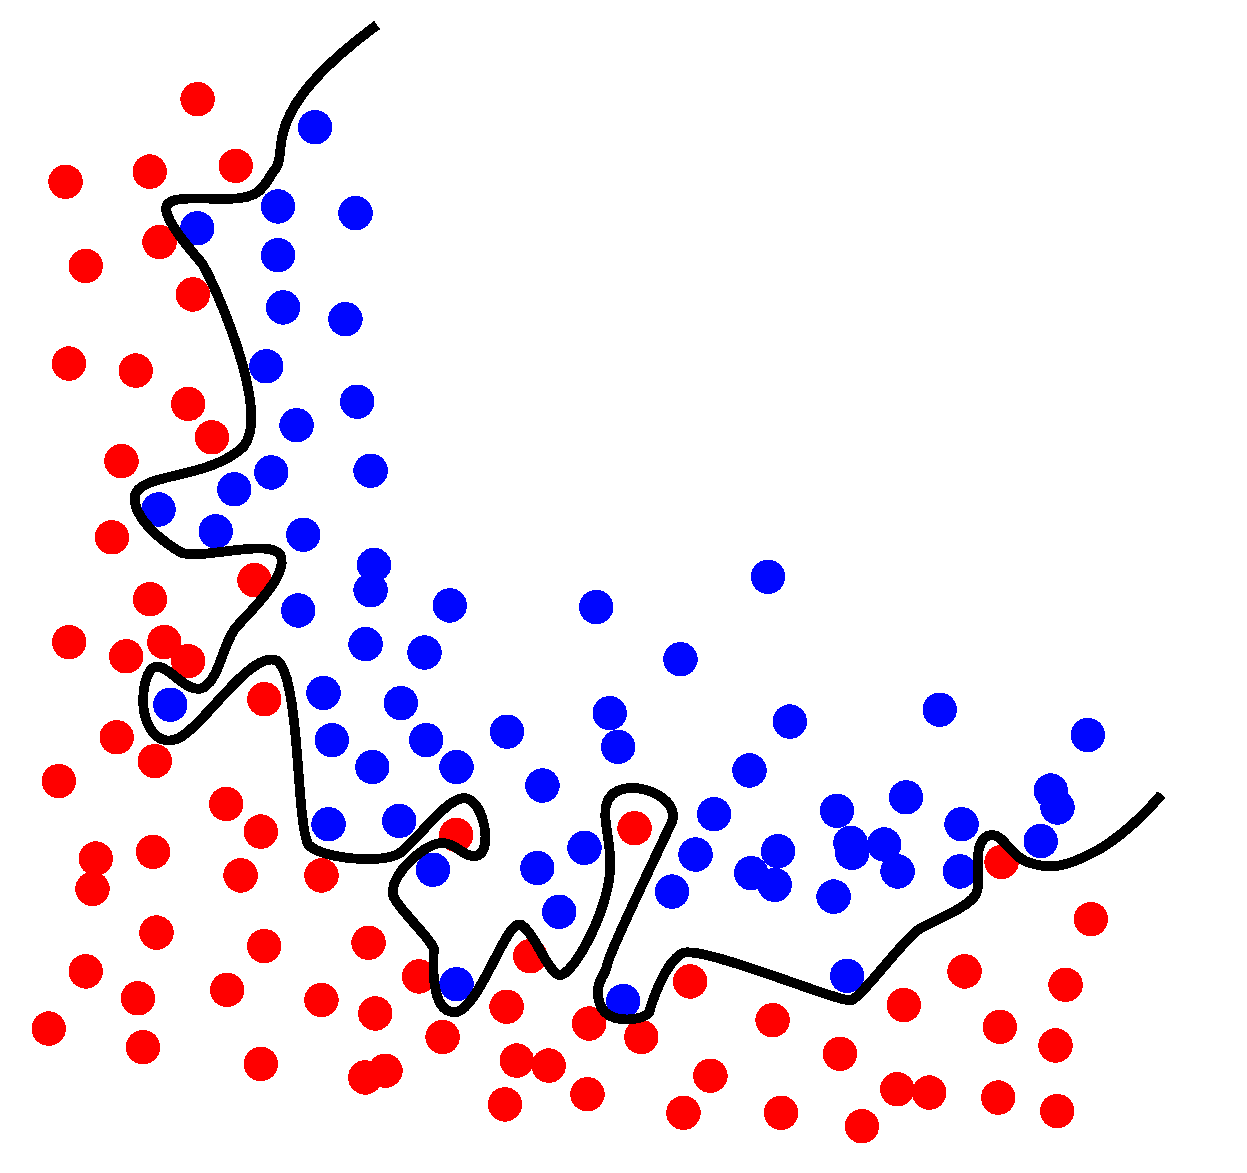
\includegraphics[clip, height=5cm]{figures/deeplearning/Overfitting.pdf}\\
    {Underfitting} &
    {Perfect Model} &
    {Overfitting} \\
    
    \end{tabular}
    }%
    \end{center}
  
  %\vspace*{-6pt}
  \caption[Overfitting Example]{This example demonstrates the effects of over- and underfitting for a 2-dimensional dataset with samples of two classes blue and red. We can see, that neither the underfitted nor the overfitted models will work well on test data, even though the overfitted model will have a 0\% error rate on the training dataset.\footnotemark}
  \label{fig:Overfitting}
  %\vspace*{-12pt}
\end{figure}

\footnotetext{Original image created by user Ignacio Icke, released under Creative Commons under \url{https://commons.wikimedia.org/wiki/File:Overfitting.svg}, edited and extend with underfitting example.}

Neural networks generally have a high tendency to overfit on the training data, because their size and the resulting number of parameters enables the network to very closely fit to the training data. When training, it usually makes sense to create a balance between the number of samples we have to train the network and the number of parameters (neurons) inside of our network. If we do not have much training data we need a smaller neural network to avoid overfitting too quickly. Overfitting is also influenced by the learning rate. If the learning rate is high enough, gradient descent will never converge completely and the network will therefore generalize better. Therefore the danger of overfitting increases when using advanced optimizers or learning rate scheduling to adapt the learning rate dynamically.

Luckily there are better ways of preventing overfitting than using a high learning rate or not use advanced optimizers. In the following we present a number of methods, which can be used in conjunction to prevent or detect overfitting.

\begin{enumerate}
  \item \textit{Early Stopping}. Before we start the training process, we can split our training data into two datasets - a training and a validation dataset. When training the neural network, we periodically test the performance of the model on the validation dataset. If the model did not improve for a certain amount of time on the validation dataset (or even gets worse) we stop training to avoid overfitting. Early stopping is very effective and easy to implement, but requires to split the training data which results in less training data for the learning process.  
  \item \textit{Regularization}. One of the best ways to prevent overfitting is to use regularization methods to keep the weights of the neural network from getting too large. To achieve this a regularization term is added to the loss function. There are three widely used methods:
  \begin{itemize}
    \item $l_2$ regularization from \textit{Ridge Regression} (also called \textit{Tikhonov} regularization) can be used to explicitly punish single large weights in the network. To achieve this a regularization term is added to the loss function which adds a weight penalty according to the $l_2$ norm:

      \[\mathcal{L}_{l_2} = \frac{\gamma}{2} \sum_{i=1}^n \theta^2_i \]

      The sum starts at $i=1$, because the bias term is usually not regularized. There also exists an alternative idea of how to implement $l_2$ regularization called \textit{weight decay} which just multiplies each weight with a constant $c < 1$ after each training step.
    
    \item $l_1$ regularization from \textit{Lasso Regression}. $l_1$ regularization also adds a term to the loss function, but this time the $l_1$ norm is used so the weights contribute equally. 

      \[\mathcal{L}_{l_1} = \gamma \sum_{i=1}^n |\theta_i| \]

      An interesting characteristic of the $l_1$ regularization is that it produces weights close to zero for the least important features. This produces a sparse model where many connections will have a zeroed out weight.
    
    \item \textit{Max-Norm Regularization} is another regularization technique which simply limits the $l_2$ norm of the connection weights $\mathbf{w}$ to a certain value, such that $|| \mathbf{w} ||_2 \leq r$. Max-Norm regularization can be implemented similar to weight decay by rescaling the weights after each training step to $\mathbf{w} \leftarrow \mathbf{w} r/||\mathbf{w}||_2$ if needed. 

  \end{itemize}
  
  \item \textit{Dropout}. Dropout is one of the latest regularization techniques which was proposed in 2012 by Hinton et al. \cite{hinton2012improving}. At each training step, every neuron (excluding output neurons) has a probability of $p$ to be ignored ("dropped out") during the current training step. The probability is usually set surprisingly high to values between 10\% and 50\%. While being simple to implement, dropout is not only a powerful regularization technique, but also makes the network more robust. 
  
  You can think about dropout in an interesting way: Since every neuron has a chance to be dropped out or be present at each training step, a network with dropout essentially represents $2^N$ distinct networks at once. The resulting network during test is composed out of all these smaller networks building a strong ensemble classifier. Neurons in the network are also less likely to co-adapt, making the network less error prone for slight input changes like noise at test time and improving overall generalization.  
\end{enumerate}



\paragraph{The Unstable Gradients Problem.}
When we talked about the backpropagation algorithm in Section \ref{sec:Backpropagation} we stated, that it is possible to train arbitrary neural networks with it, regardless of the number of layers. While this is true to some extend the backpropagation algorithm initially struggled to train networks with more than three layers. Since the gradients are computed layer-wise and propagated backwards from the outputs to the inputs using the connection weights, the gradient between the layers $i$ and $j$ (meaning layer $i$ is the input layer to layer $j$) shrinks or grows depending on 

\[F_{i,j} = ||\phi(v_j) \cdot \mathbf{w}_{i, j}||_1\]

This means, that if $F_{i, j} < 1$ the gradients tend to get exponentially smaller for each layer which is called the \textit{vanishing gradients problem} and if $F_{i, j} > 1$ the gradients tend to exponentially grow which is called the \textit{exploding gradients problem}. Both problems lead to networks, which contain upper layers which do not learn anything and are therefore often worse in performance than networks with less layers.

To prevent the gradients from exploding or vanishing, we need to look at both, the activation function and the weights. As for most problems, there are multiple solutions which can be used standalone or in conjunction with others, to enable the BP algorithm to properly work for deep neural networks:

\begin{enumerate}
  \item \textit{Non-Saturating Activation Functions.} We already presented a number of activation functions in Section \ref{ssec:ActivationFunctions}. The initially used sigmoid activation function had two crucial problems for its application in deep neural network. First, its slope is at most 0.25, which means errors in backpropagation always tend to get smaller with each layer. Second, the function saturates to 0 and 1 for very small or very large inputs, leading to very small gradients at these points and thus very slow learning. The solution is to use one of the other activation functions which do not saturate to a maximum value. Therefore deep neural networks usually use either ReLU, Leaky ReLU, ELU or SELU activations. 
  \item \textit{Improved Network Weight Initialization.} In 2010 Glorot and Bengio proposed a way to deal with unstable gradients, by using a new method to initialize the weights \cite{glorot2010understanding}. Usually weights in neural networks were randomly initialized with a normal distribution with a mean of 0 and a standard deviation of 1. Glorot and Bengio showed, that for backpropagation we need to control the variance of the outputs of each layer in both directions - for the forward pass and for the backpropagation. This means, that the output distribution of each layer should have equal variance to the input distribution and at the same time we need the variance of the gradients needs to be the same before and after each layer. Completely satisfying this constraint is only possible if two adjacent layers have the same number of neurons, but the initialization can still be optimized. If we denote the number of input neurons by $fan_{in}$, the number of output neurons by $fan_{out}$ and the average number by $fan_{avg} = (fan_{in} + fan_{out}) / 2$, the Glorot initialization is given by 

  \begin{align*}
    &\text{A normal distribution with mean 0 and variance } \sigma^2 = \frac{1}{fan_{avg}} \\
    &\text{Or a uniform distribution between -r and +r, with } r = \sqrt{\frac{3}{fan_{avg}}}
  \end{align*}
  
  This initialization strategy has proven to successfully minimize effects of the unstable gradients problem at the beginning of training. Depending on the used activation function, the initialization strategy needs to be adapted slightly. ReLU and ELU activation functions use the so-called He initialization with $\sigma^2 = 2 / fan_{in}$ and the SELU activation function uses the LeCun initialization with $\sigma^2 = 1 / fan_{in}$.
  \item \textit{Batch Normalization.} The problem with a good initialization of the network is, that the problem is only prevented from appearing directly at the start of the training process. Therefore in 2015 Ioffe and Szegedy proposed to a new techniques called \textit{Batch Normalization} (BN) to keep the output of each layer normalized with respect to some distribution. Their algorithm adds an additional operation before (or after) the activation function of each layer to zero-center, scale and shift the input for each layer. The parameters for the shift and scaling operations are learned at training time by computing an average over the current minibatch (therefore the name \textit{batch} normalization). The input for each layer can then be calculated in four steps:


  \begin{enumerate}\setcounter{enumii}{0}\renewcommand\theenumii{\arabic{enumii}}
    \item Calculate the mean input vector over the minibatch $B$: $\displaystyle \mu_B = \frac{1}{m_B} \sum_{i=1}^{m_B} x^i$ 
    \item Calculate the standard deviation over the minibatch $B$: $\displaystyle \sigma_B^2 = \frac{1}{m_B} \sum_{i=1}^{m_B} \left(x^i - \mu_B\right)^2$
    \item Calculate zero-centered and normalized input vectors: $\displaystyle \hat{x}^i = \frac{x^i - \mu_B}{\sqrt{\sigma_B^2 + \epsilon}}$
    \item Calculate rescaled and shifted outputs: $\displaystyle z^i = \gamma \otimes \hat{x}^i + \beta$
  \end{enumerate}
  
  The scaling parameter $\gamma$ and the shift parameter $\beta$ are learned via backpropagation together with the other variables of the neural network. Because $\mu_B$ and $\sigma_B$ are only calculated for the current batch, it is not ideal to use them at test time. Instead they are usually calculated by either recalculating them over the whole training dataset, or to calculate them at training time by using a running mean. Batch normalization significantly improves the performance of deep neural networks, but adds additional complexity at both training and test time.
  \item \textit{Gradient Clipping.} To avoid overhead like in batch normalization, an easy way to deal with exploding gradients is to just clip the value of the gradients to be in a certain range, e.g in $[-1, +1]$. This was first used by Razan et al. in 2013 for the training of recurrent neural networks, which are complicated to combine with batch normalization \cite{pascanu2013difficulty}. To keep the direction of the gradient it is also possible to clip by normalizing the gradient vector to the $l_2$ norm.
  \item \textit{Residual Networks.} Another take on the unstable gradients problem is the use of residual neural networks. These networks contain skip connections (shortcuts) which directly feed the output of one layer to another layer which is not its direct successor. Figure \ref{fig:ResidualBlock} shows a residual building block for a network. 
  
  \begin{figure}[t]
    
    \begin{center}
        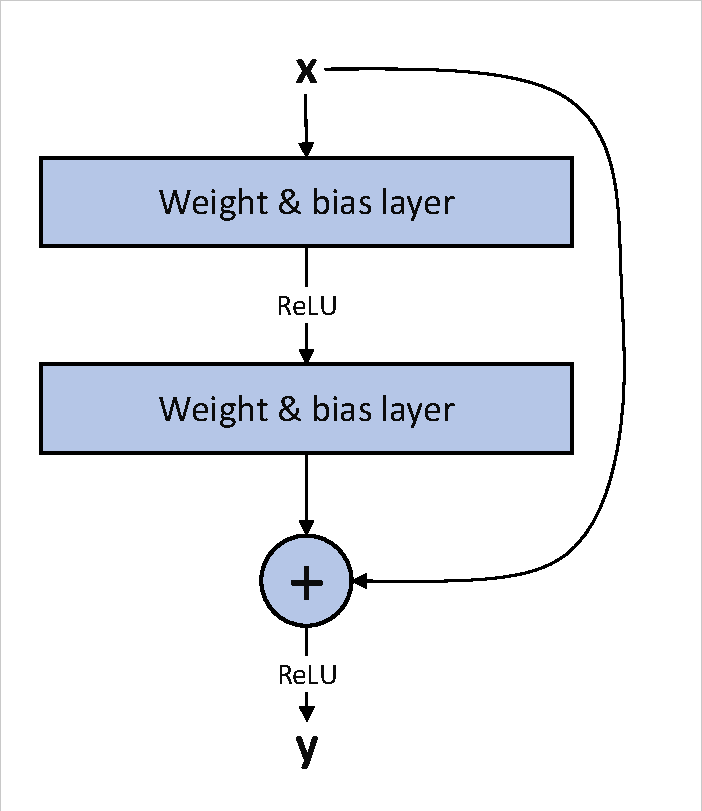
\includegraphics[clip, trim=10px 10px 10px 10px, width=0.4\columnwidth]{figures/deeplearning/Residual_Block.pdf}
    \end{center}
    
    %\vspace*{-6pt}
    \caption[Residual Block]{The structure of a residual block. Deep neural networks without skip connections are not able to learn the identity for a layer when trained with BP. Therefore larger networks often perform worse than shallower ones. With skip connections, networks can learn deviations from the identity, which works far better and also eliminates unstable gradients.}
    \label{fig:ResidualBlock}
    %\vspace*{-12pt}
  \end{figure}

  Skip connections are motivated by biological structures in the cerebral cortex. In 2016 Xu et al. first used residual connections in artificial neural networks for image recognition \cite{he2016deep}. They showed, that large networks with residual connections are faster to train and yield better end results without batch normalization. By skipping layers, the network is able to propagate errors from the output directly into layers close to the input of the network, allowing networks which have hundreds of layers. Having lower level features at later stages of deep networks also seems to be beneficial for the overall performance.
\end{enumerate}

\section{Specialized Network Structures} \label{sec:SpecializedNetworks}
Until now we only were working with fully connected feed forward networks. While every fully connected layer is able to model any other arbitrary connection with the next layer, it is faster to train networks which already contain a certain structure, if that structure directly benefits the task. Especially image recognition has shown to be hard, even for larger multilayer networks. Therefore a special architecture is used when dealing with pixel inputs which we will explore in Section \ref{ssec:CNNs}. Sometimes we are also confronted with continuous input data which requires memory. To deal with time dependent input data, another special network architecture exists, which we will take a look at in Section \ref{ssec:RNNs}. 

\subsection{Recurrent Neural Networks} \label{ssec:RNNs}
Feed forward neural networks are great for making predictions on data without a time component, e.g. images classification tasks. But if you want to predict the future, you often need to remember the past. And that is one thing our networks are missing: A memory. Think of a self-driving car, which has to keep track of all its surroundings. A pedestrian might walk on the sidewalk and at some point get obscured by a parking car. If we remember that we saw that pedestrian some time ago, we can expect him to suddenly reappear and maybe cross the road. This is especially important if our pedestrian is a child which might not watch out for a car. A normal feed forward network would forget about the child as soon as it can not see it anymore, but if we had some kind of memory we would be able to remember the child and slow down. This situation cannot always be solved by adding timed information as input to the neural network (e.g. having a sequence of images from a video stream as input rather than a single image) as we do not know ahead of time for how long our memory has to last. 

\begin{figure}[ht]
    
  \begin{center}
      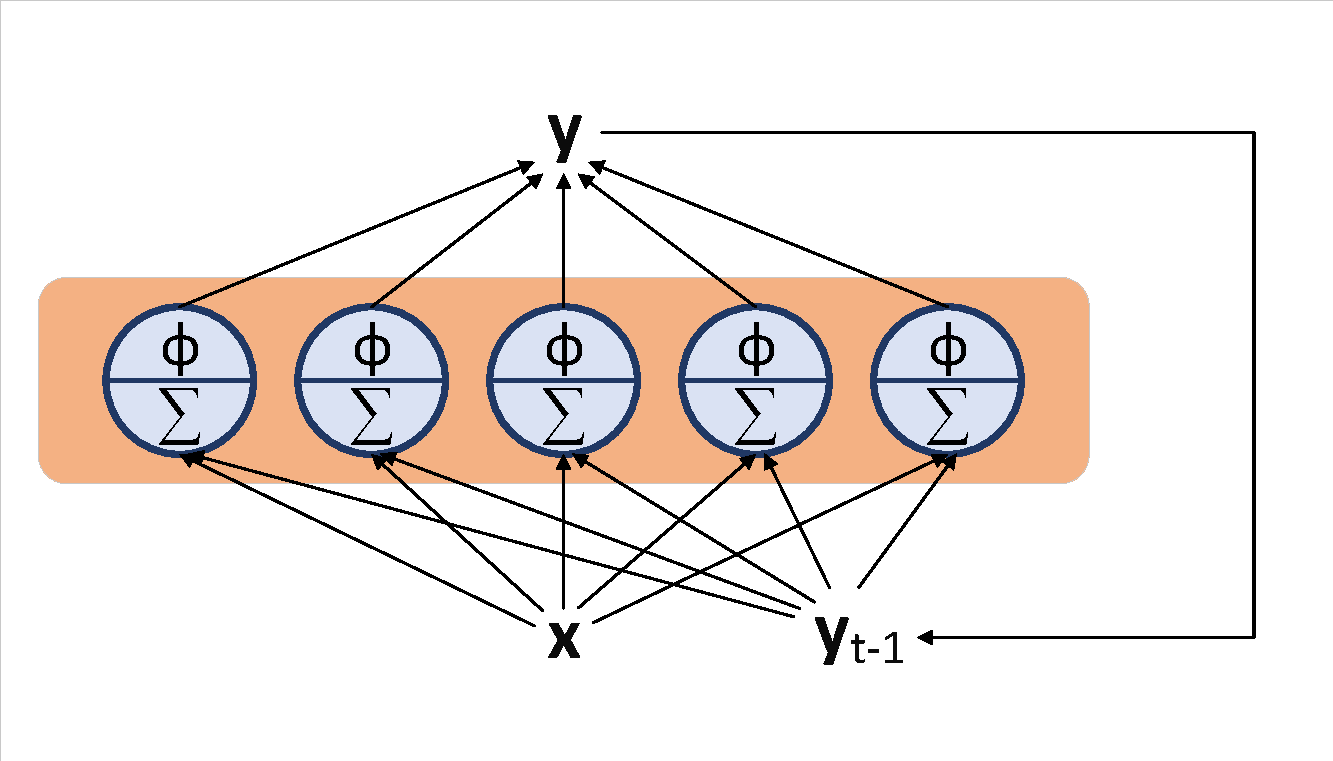
\includegraphics[clip, trim=10px 10px 10px 10px, width=0.7\columnwidth]{figures/deeplearning/Recurrent_Layer.pdf}
  \end{center}
  
  %\vspace*{-6pt}
  \caption[Recurrent Layer]{A layer in a recurrent neural network. The output $\mathbf{y}$ of the layer is used as a input for the next timestep.}
  \label{fig:RecurrentLayer}
  %\vspace*{-12pt}
\end{figure}

To solve this problem, we modify the neurons of our network. Instead of having only a single flow direction from the input to the output, our new network also has connections pointing backwards. This type of network is called a \textit{recurrent neural network} (RNN). Usually each layer of a RNN takes its own output as additional input vector in the next time step. This way, the network is able to remember its past inputs and its decisions at the same time. We included a representation of a recurrent layer in Figure \ref{fig:RecurrentLayer}. At step $t$ each recurrent neuron receives two input vectors: The current input vector $\mathbf{x}_t$ and its own output vector of the previous step $\mathbf{y}_{(t-1)}$. Accordingly each recurrent neuron has two sets of weight vectors $\mathbf{w}_x$ and $ \mathbf{w}_y$. If we look at the whole layer of neurons and their weights $\mathbf{W}_x$ and $\mathbf{W}_y$ we can compute the layer output by 

\[\mathbf{y}_t = \phi(\mathbf{W}_x^T \mathbf{x}_t + \mathbf{W}_y^T \mathbf{y}_{(t-1)} + \mathbf{b})\]

Recurrent neural networks are harder to train than regular feedforward networks, but essentially still rely on classical backpropagation. The trick is to unroll the network through time and then train it using regular backpropagation. This method for training RNNs is called \textit{backpropagation through time} (BPTT). BPTT unrolls the network for a fixed number of timesteps $T$ into the past. The first recurrent vector is set to 0 and the output of each unrolling step is evaluated by a cost function. The gradients of the cost function are then backpropagated through the unrolled network, so the weights and biases are actually updated multiple times for a single learning step. 

Recurrent neural networks can be used for a multitude of tasks which require time series data. They are especially well suited for natural language recognition, processing or translation as well as forecasting of future sequences (e.g. stock market prices) or the processing of video input. Since training of RNNs is hard because the unrolling process produces very deep network structures, often a modern improved version of RNNs called \textit{long short-term memory} (LSTM) is used, which was developed in 1997 by Hochreiter and Schmidhuber \cite{hochreiter1997long}. LSTMs implement a completely new and complex model for a single neuron which allows it to remember information for longer periods of time and be trained more efficiently.


\subsection{Convolutional Neural Networks} \label{ssec:CNNs}
Although many tasks can quickly be solved by standard feedforward neural networks, performing tasks on images proofed to be notoriously hard. While detecting objects in a picture seems to be effortless for humans, machine learning struggles with every aspect of image recogition. But what makes the task so easy for humans and so difficult for machines? Since humans (and most other animals which live on land) rely on their ability to see, they developed a complex preprocessing pipeline which allows them to see, without learning how to see. Before the signals from our eye reach our visual cortex, they are preprocessed and already transformed into high-level features. Our brain therefore never needs to deal directly with the raw signals from our retina. Even though our brain is incredibly powerful, this preprocessing allows it to handle images in a fast and reliable way (well most of the time, since the preprocessing is also responsible for how many optical illusions work). 

In 1958 and 1959 David Hubel and Torsten Wiesel experimented with cats to understand how their visual cortex works \cite{hubel1959single, hubel1959receptive}. They found out, that neurons that are directly connected to the retina only react to local stimuli on a specific region. They also were able to show, that certain neurons only react to images of horizontal lines, while others only react to lines with different orientations. Later neurons then combine these lower level features and only react to complex features build from these lower level patterns. In 1998 LeCun et al. were able to adapt this structure for artificial neural networks in their \textit{LeNet-5} architecture \cite{lecun1998gradient} which is the first \textit{Convolutional Neural Network} (CNN). CNNs introduce two new building blocks which build the foundation of modern image recognition: The \textit{convolutional layer} and the \textit{pooling layer}.

\paragraph{Convolutional Layers.} Convolutional layers resemble their biological counterparts by not being fully connected. Instead each neuron of the convolutional layer is only connected to a small region on its input layer. This means each neuron only reacts to local signals of a specific $n \times m$ region inside of the previous layer. Each additional layer therefore learns higher level features, based on the lower level ones from the previous layer. In Figure \ref{fig:ConvolutionalConnections}, we show an example of a convolutional layer. The neuron in the $i$th row and $j$th column is connected to the neurons of the previous layer in a window with size $f_h \times f_w$ and centered at $(i, j)$. To avoid each layer from getting smaller than the previous one, the layer can be padded with zeros. If the layer instead should reduce the complexity, the windows can be used with a stride $s$ to achieve a downscaling effect. The stride defines how far the window is shifted between two neurons.  

\begin{figure}[ht]
    
  \begin{center}
      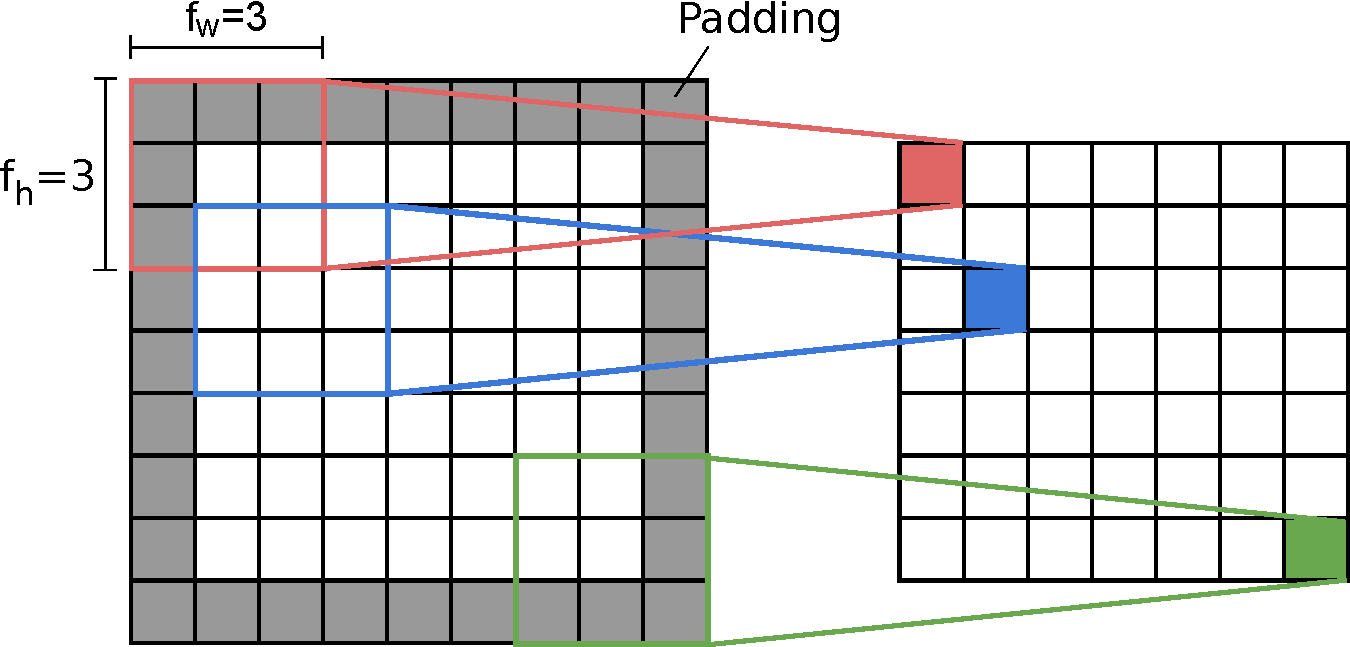
\includegraphics[clip, width=0.7\columnwidth]{figures/deeplearning/Convolution.pdf}
  \end{center}
  
  %\vspace*{-6pt}
  \caption[Convolutional Connections]{Connections in a convolutional layer with a window of $3 \times 3$ and a stride of 1. The input is padded to avoid downscaling. Neurons are only connected locally with rectangular receptive fields.}
  \label{fig:ConvolutionalConnections}
  %\vspace*{-12pt}
\end{figure}

An important idea when using convolutional networks is, that a feature that is interesting in one area (e.g. horizontal lines) may also be interesting in every other area of the input image. We call the neurons whose weights compute a specific feature a \textit{filter} or \textit{kernels}. If we use the same weights and biases of the filter for the whole layer (called \textit{weight tying}), the output of the layer is a \textit{feature map}. This feature map contains the output of a filter placed at every position at the previous layer. To allow the network to learn multiple filters, a layer in a convolutional network is a stack of feature maps generated by multiple filters. Each feature map is connected to the full depth of all feature maps of the previous layer. For example if we have an $100 \times 100$ RGB image (3 channel input) and construct $20$ filters with size $5\times 5$, every neuron of the first convolutional layer will be connected to $5\times 5 \times 3 = 75$ input neurons. The layer then will output 20 images of size $100 \times 100$ as output, one for each filter. Filters of size $5\times 5$ of a second convolutional layer will therefore work on a input size of $5\times 5 \times 20 = 500$ values.

The fact that each filter only needs to be trained once while being able to use it on every part of the input image produces a large advantage compared to fully connected layers. Its internal structure allows the CNN to vastly reduce the number of parameters needed to express a filter operation over the complete image. The only downside is, that a CNN produces large intermediate results, because each filter outputs a complete copy of the image which needs a lot of memory.

\paragraph{Pooling Layers.} Pooling layers work similar to convolutional layers only on a local part of the input, but serve a different function. Pooling layers \textit{subsample} (i.e. shrink) the input. We already saw, that our intermediate results get pretty large, so by downscaling them, we are able to save computational resources, reduce memory usage and also reduce the numer of parameters (which prevents overfitting). Pooling layers also introduce invariance against small translations in the input image. 

\begin{figure}[ht]
    
  \begin{center}
      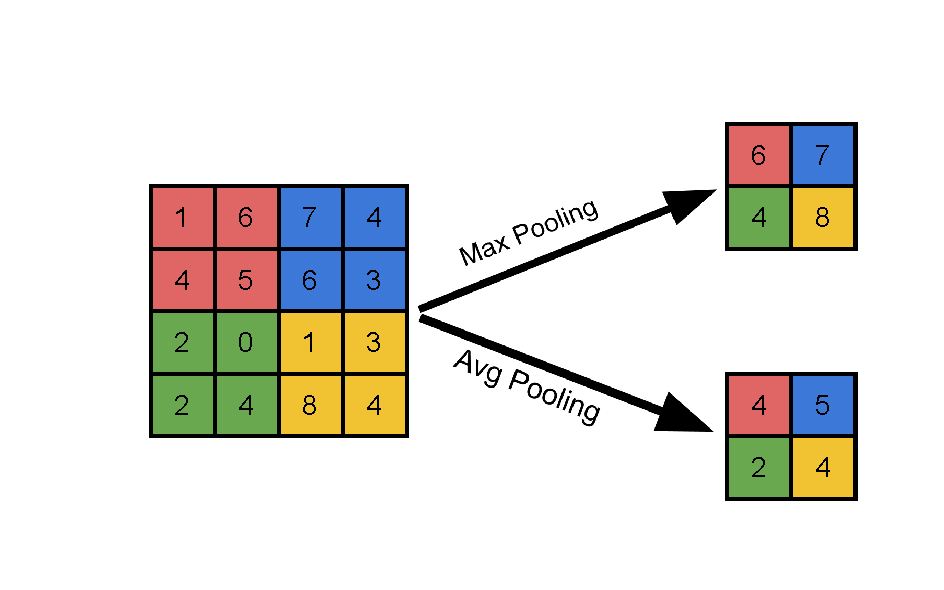
\includegraphics[clip, width=0.7\columnwidth]{figures/deeplearning/Pooling.pdf}
  \end{center}
  
  %\vspace*{-6pt}
  \caption[Pooling Layer]{A Pooling Layer with size $2 \times 2$ and a stride of 2. The output on the top represents max pooling the output on the bottom average pooling.}
  \label{fig:Pooling}
  %\vspace*{-12pt}
\end{figure}

Let us look at how pooling layers work. Like convolutional layers they are only connected to a small rectangular receptive field, but they typically do not connect to the full depth of the previous layer - they only subsample the individual "images". Pooling layers have no weights associated to them. Instead they use a pooling function to aggregate the inputs. Usually the \textit{max} or the \textit{mean} function is used. Figure \ref{fig:Pooling} shows an example of a pooling layer with $2 \times 2$ kernels with a stride of 2. On the top we have the output of a \textit{max pooling layer}, which means that out of four values from the input image only the maximum will be propagated to the next layer and on the bottom is the output of a \textit{average pooling layer} which averages over all its inputs. While earlier networks often used average pooling, nowadays often only max pooling is used. 

\begin{figure}[ht]
    
  \begin{center}
      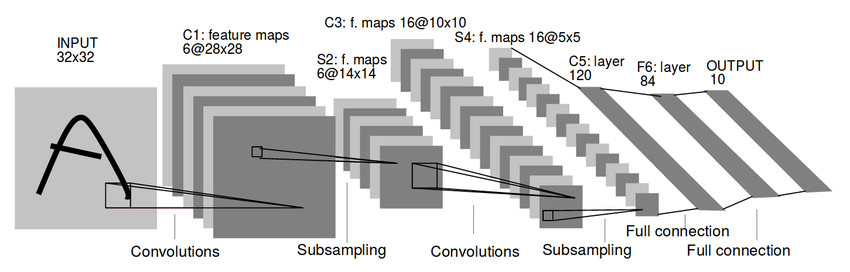
\includegraphics[clip, width=0.7\columnwidth]{figures/deeplearning/LeNetArch.png}
  \end{center}
  
  %\vspace*{-6pt}
  \caption[LeNet-5 Architecture]{The architecture of the first CNN LeNet-5 \cite{lecun1998gradient}. It was designed to recognise handwritten digits and used two convolutional and two pooling layers.}
  \label{fig:LeNet}
  %\vspace*{-12pt}
\end{figure}

Pooling layers typically use a stride which is equal to their own size. While pooling is very useful to save computational resources, pooling larger areas than $2 \times 2$ can lead to information loss, so pooling has to be used carefully. However in current CNN architectures, pooling layers are used after every convolutional layer. By using this structure the intermediate results get smaller and smaller and the repeated pooling results in a larger invariance against pixel shifts or even smaller rotations in the input image. 

Convolutioal networks usually end with one or more fully connected layers. We included a sketch of the original LeNet-5 architecture in Figure \ref{fig:LeNet} which demonstrates a typical CNN. Modern architectures are often larger in every aspect and often use convolutional layers in conjunction with residual connections to allow efficient training of very deep networks. Recent papers also suggest to only use convolutional layers (\textit{Fully Convolutional Networks} (FCNs)) for specific tasks like object detection \cite{long2015fully}. To further improve invariance against scaling and rotation, the feature output of multiple convolutional layers can be directly combined, which is called Feature Pyramid Network (FPN) \cite{lin2017feature}. 


% \section{Current Research} \label{sec:NNResearch}
% Since its rebirth around 2010, deep learning has been a field of extensive research with hundrets of papers published every years. Nowadays, deep learning techniques are incorporated into many end-user applications, especially when it comes to human interaction like speech recogition or search engines. Deep learning is also heavily used for modern automation tasks like self-driving cars. The large interest in improving these technologies has led to a situation, where records are broken every year and techniques quickly become outdated or at least develop into something more refined. In this Section we want to give some short insight    


\chapter{Reinforcement Learning} \label{chp: RLOverview}
In this chapter we want to give an overview over existing methods for reinforcement learning. RL algorithms can be grouped into multiple families. We provide an overview over some of the most popular algorithms from each family in Figure \ref{fig:rl_families}. Because many algorithms are modular an accurate taxonomy of RL algorithms is difficult. For now we divide the algorithms into three basic groups - the value-based, the policy-based and the model-based methods. While model based methods try to model (or start with a model of) the environment they have to make predictions for to improve their accuracy, value- and policy-based methods do only learn to make predictions for actions in the environment without actually modeling it.
Over the years these basic algorithms were (partially) combined into methods which inherit ideas from multiple basic groups. One the one hand we mainly have variants of the actor-critic algorithm which all combine value-based and policy-based methods. On the other side we have various combinations of value-based or policy based methods mixed with ideas from the model-based family. For example the earlier mentioned AlphaZero algorithm uses value estimation in combination with \textit{Monte Carlo Tree Search} \cite{silver2017mastering}. 

\begin{figure}[ht]
    
  \begin{center}
      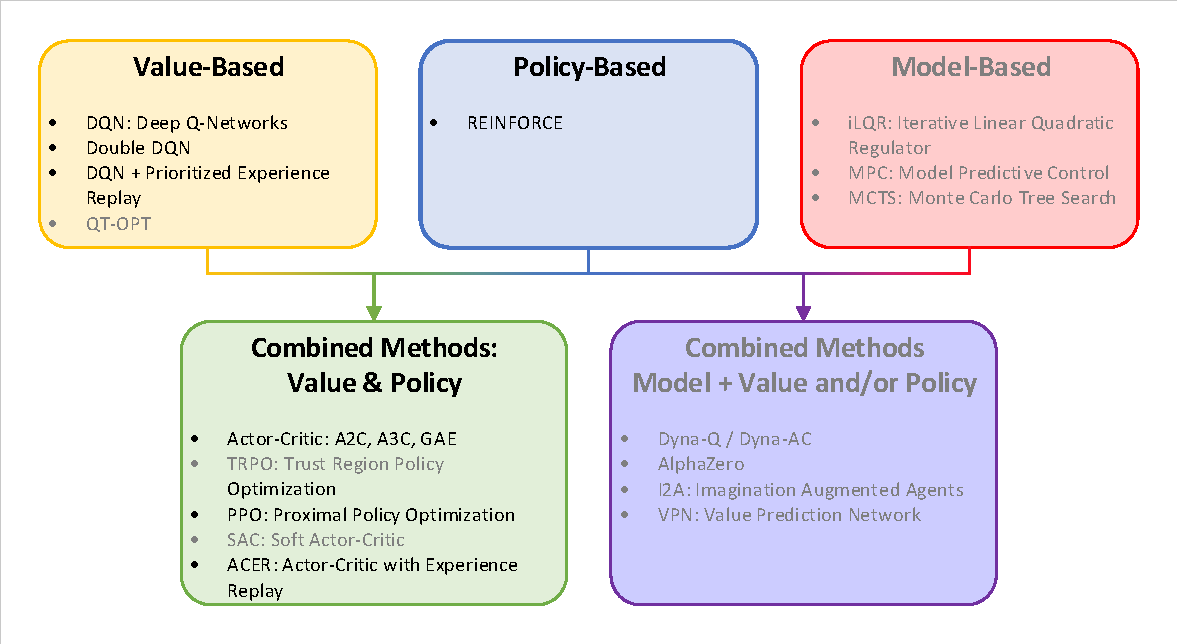
\includegraphics[clip, trim=10px 10px 10px 10px, width=0.95\columnwidth]{figures/rl/rl_families.pdf}
  \end{center}
  
  %\vspace*{-6pt}
  \caption[Overview of RL Families]{Overview of reinforcement learning families (adapted and extended from \cite{foundations2019graesser}). Methods that will not be used in this work are greyed out.}
  \label{fig:rl_families}
  %\vspace*{-12pt}
\end{figure}

In this work we will be focusing on actor-critic variants and value-based algorithms, so we will not cover model-based algorithms here. However we will be taking a look at policy-based methods, since they provide basic building blocks for the algorithms we will be using. \\ 
In this chapter we will begin with some basic ideas and challenges of reinforcement learning, as well as with some mathematical foundations in Section \ref{sec:concepts}. After that we will continue by introducing our first family of RL algorithms the value-based methods in Section \ref{sec:ValueMethods}. We will continue with a short overview over the idea of policy-based algorithms in Section \ref{sec:PGMethods} and will finally cover combined algorithms in Section \ref{sec:CombinedMethods} where we will focus on the actor-critic method and its successors.

\section{Key Concepts} \label{sec:concepts}
In this Section we give some basic insight into key concepts of reinforcement learning. First we give some basic intuition into how reinforcement learning works and what the challenges are when learning behavior from an unknown environment in Section \ref{ssec:rlidea}. We then continue by defining some of the basic terminology in Section \ref{ssec:rlterms} and finish with a different look on the RL problem from a mathematical point of view in Section \ref{ssec:RLMDP}.  

\subsection{Basic Ideas and Challenges} \label{ssec:rlidea}

Reinforcement learning at its core tries to solve some arbitrary decision-making problem. This problem is given by an \textit{environment} which produces information about its \textit{state} in form of an \textit{observation}. At each timestep an \textit{agent} receives the current observation and then acts according to some \textit{policy} by choosing from a set of available \textit{actions}. These actions should ultimately lead to the achievement of some objective inside of the environment. The behavior of the agent usually is encouraged by some kind of \textit{reward} which is returned by the environment. This basic agent-environment interaction loop is shown in Figure \ref{fig:rl_control_loop} \\ 

\begin{figure}[ht]
    
  \begin{center}
      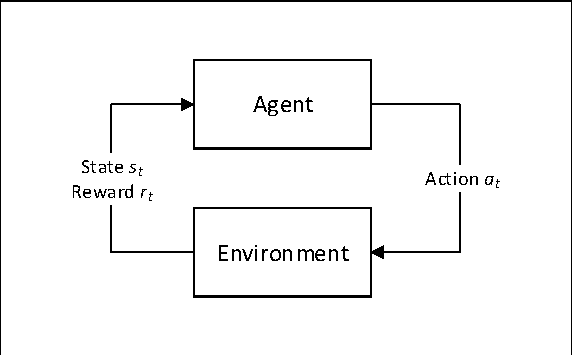
\includegraphics[clip, trim=10px 10px 10px 10px, width=0.6\columnwidth]{figures/rl/rl_control_loop.pdf}
  \end{center}
  
  %\vspace*{-6pt}
  \caption[Agent-environment interaction control loop]{The basic reinforcement learning control loop for agent-environment interaction.}
  \label{fig:rl_control_loop}
  %\vspace*{-12pt}
\end{figure}

This abstract setting can be used to solve a variety of tasks. We have three examples given in Figure \ref{fig:RLExamples}.
\begin{enumerate}
  \item \textbf{Playing the game Breakout.} Breakout is a game from the game console Atari. The goal of the game is to break the bars at the top, by reflecting a moving ball with a paddle at the bottom (like in Ping Pong). The observation is an rgb image of the game itself and the possible actions include resetting or firing the ball as well as moving the paddle to the left or right side of the screen. The reward is the current game score, which increments with every broken piece of barrier at the top. 
  \item \textbf{Playing the game of chess.} The input might be a complex representation of the positions of all pieces, or just a plain rgb-image. The possible actions change after every move, because they are dependent on the valid moves of all pieces. Reward might be as simple as winning ($+1$) or loosing ($-1$) the game, but can be more complex.
  \item \textbf{Grasping objects in a container.} A robotic arm should be trained to grasp arbitrary objects in a container. The observation is a plain image captured from above the robotic arm and a positive reward is given if the robot is able to successfully grasp an object. Actions include positioning the robot arm and opening or closing the "hand". 
\end{enumerate}

\begin{figure}[ht]
  \begin{center}
  \resizebox{0.95\columnwidth}{!}{%
  \begin{tabular}{ccc}
    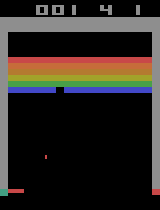
\includegraphics[clip, height=5cm]{figures/rl/Breakout.png}  &
  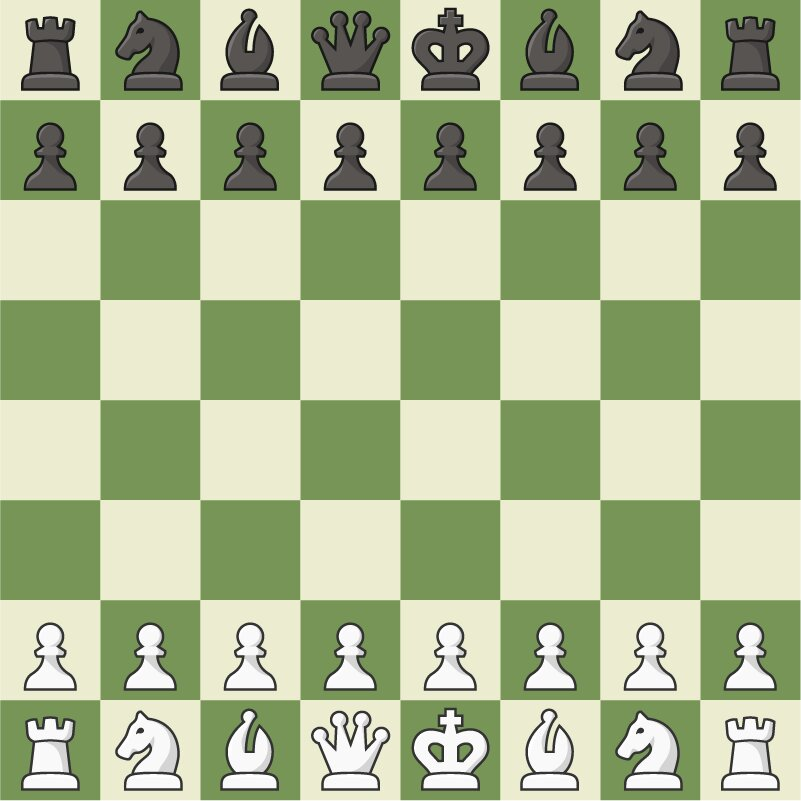
\includegraphics[height=5cm, keepaspectratio]{figures/rl/chess.jpg} & 
  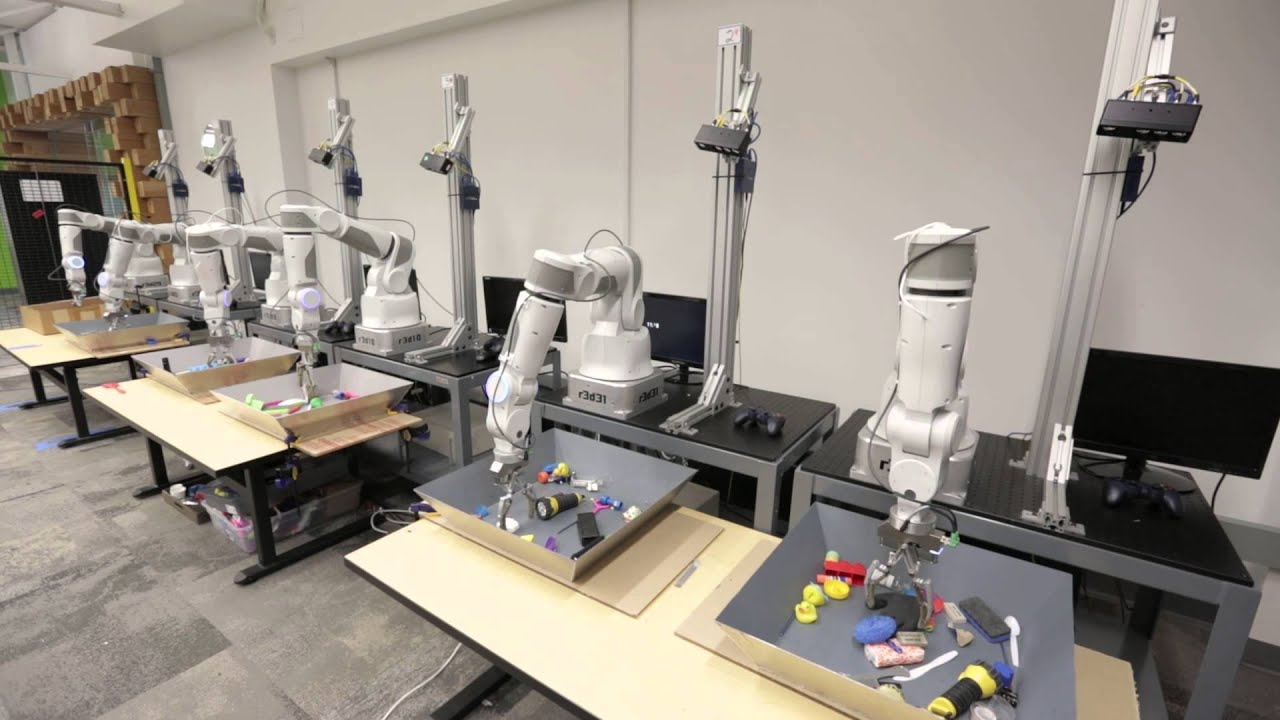
\includegraphics[trim=400px 0px 75px 0px, clip, height=5cm, keepaspectratio]{figures/rl/Google_Robot_Learning.jpg}\\
  {(a) The Atari game Breakout} &
  {(b) Chess\footnotemark} &
  {(c) Google Robot Grasping \footnotemark}\\
  
  \end{tabular}
  }%
  \end{center}
  %\vspace*{-12pt}
  \caption{Reinforcement learning examples.}
  \label{fig:RLExamples}
  %\vspace*{-12pt}
\end{figure}
  
\footnotetext{Image from chess.com \url{https://www.chess.com/bundles/web/images/offline-play/standardboard.6a504885.png}}
\footnotetext{Image from ai.googleblog.com \url{https://i.ytimg.com/vi/iaF43Ze1oeI/maxresdefault.jpg}}

Let's take a closer look at another example, pictured in Figure \ref{fig:CartPole}: The game of balancing a stick on a cart in a 2D environment. The sick can only be balanced by moving the cart, which has some velocity and can either be accelerated to the left or to the right. At each timestep the agent gets an observation which describes the current position and angle of the sick and can then choose which action it wants to take. If the stick falls over the agent looses. If it is able to balance the stick for more than 200 steps it wins. At each step it survives it gets a reward of $+1$. \\
Balancing a stick is harder than it initially seems to be. A simple algorithm which always moves the cart towards the direction the stick is leaning to, will always overshoot after a short time and loose balance. Of course we can think of a more complex algorithm and maybe solve the problem this way, but what if we want the computer to figure things out? How can we implement an algorithm which figures out on its own which actions should be taken for some given observation? How would we ourselves solve this problem? The answer is simple try and error. A human learns how to balance a stick, by balancing it. This will of course fail at the beginning, but after some time a human would get better and better at \textit{estimating} how the stick behaves in response to the actions that were taken. Similarly our reinforcement learning algorithm should just play around and looks at the results. Did the stick fell over? How long were we able to balance the stick? At which point did it fell and which actions led to that outcome? If we can answer all these questions we might be able to learn how to solve the problem. \\

\begin{figure}[ht]
  
  \begin{center}
      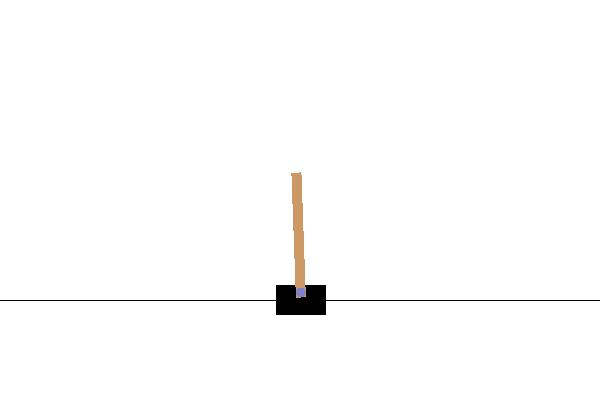
\includegraphics[trim=0px 50px 0px 100px, clip, width=0.6\columnwidth]{figures/rl/CartPole.jpg}
  \end{center}
  
  %\vspace*{-6pt}
  \caption[CartPole Environment]{A classic toy example from OpenAI gym \cite{openAIgym}: The CartPole environment.}
  \label{fig:CartPole}
  %\vspace*{-12pt}
\end{figure}


Building an association between some action and the resulting outcome in the environment is actually one of the greatest challenges for RL algorithms and known as the \textit{credit assignment problem}. Since rewards are typically sparse and delayed, understanding their origin is hard. Especially if you think about more complex games like chess, it is really unclear to what extend which move was responsible for winning or loosing a game. This problem becomes even greater the more sparse the rewards get: If we only reward winning or loosing, figuring out what made us win or loose is pretty hard, but if we reward or punish every single action, we might end up with a copy of an already known strategy. The challenge is to create an unbiased reward signal which does not distort the learning process. In the case of balancing a stick this is easy. Balancing the stick for a longer time is always good and can be rewarded. But as problems become more complex it is unclear if an action is actually good. If we take another look at chess for example, it might be beneficial to take a piece of your opponent, but it might also be better to go for a check or something which just gives you a positional advantage. Which action should be rewarded to what extend? In the end it is also a balance with how much time there is to learn. Sparse rewards will always result in longer training times, but give more freedom and thus might yield better results. \\
In the presence of sparse rewards another challenge arises: What if our learning algorithm is not able to find any solution at all? How can the algorithm know that there is a better solution out there, than the solution it already found? The answer is it cannot. The observations the agent makes in the environment are dependent on the taken actions. If the agent chooses the wrong actions it might never be able to explore the environment to a point where it receives more reward. The agent might get stuck with the false impression that it already achieved the maximum reward that is possible. \\
The last challenge we want to talk about is closely connected to the second one: Keeping the balance between exploration of the environment and exploitation of already learned behavior. Often diverging from already proven behavior decreases the short-term reward, but might lead to a much larger reward in the future. People face this problem in their everyday life: If you know the route from your home to some place, you are way more likely to take that route, than trying to find a shorter one, but risking the eventual failure. In this scenario the person - or in RL the agent - might get stuck in a situation where it never does anything else than taking the best known route, and get forever stuck in this local optimum.

\subsection{Terminology} \label{ssec:rlterms}
We already talked a lot about the existing challenges of reinforcement learning. Before we want to dive deeper into the various techniques that were developed to overcome these problems, we want to take a short look on the common terminology used throughout these algorithms.

\paragraph{States and Observations.}
For every environment there is a difference between the internal state $s$ of the environment and the observation $o$ an agent receives. While the state covers all information about the "world" the environment represents, the observation is a representation of that world and may or may not contain all information.  In the remainder of this chapter we will often use $s$ instead of $o$, but it should be clear from context, if an observation or the internal state is referenced. 

Depending weather we can observe the whole environment or not, we talk about fully or partially observed environments. Observations are typically given to the agent as a real-valued vector.

\paragraph{Actions.}
Actions are the things an agent can do in the environment. Most of the time they are fairly simple, like deciding to go left or right, but they can be more complex.

The set of actions an agent can perform in an environment is usually called the \textit{action space}. Depending on the environment, the action space might be discrete - with only a finite number of available choices - or continuous. Discrete action spaces are typical for game-like environment like CartPole or Breakout. Usually discrete actions are mutually exclusive, meaning only a single action can be chosen at a time: We can not go left and right - we have to choose.

Continuous action spaces on the other hand allow for a value attached to each available action and are often found in robot control tasks. For example if we look at a self-driving car, we have an action for the degree of the steering wheel and an action for the position of each pedal which need to be set in each step.

Not all RL algorithms are able to handle both types of action spaces. In some instances it is possible to transform continuous action spaces into discrete action spaces if no absolute precision is necessary. However this often results in a very high number of available actions.

\paragraph{Policies.}
Most of the time the words agent and policy will be used in the same manner. For the sake of clarity we want to define the policy as the rule(s) an agent uses to decide which action should be taken for some observation. We can think of the policy as the actors brain.

We denote the policy by $\mu$ if it is deterministic and $\pi$ if it is stochastic. Later when we are focusing on deep RL all of our policies will be build from artificial neural networks which are parameterized by their weights and biases. We therefore extend our notion to include these parameters as $\theta$ to have parameterizable policies $\mu_\theta$ and $\pi_\theta$. If the agent receives an observation at time $t$ it then generates the action according to its policy by:
\begin{align*}
  a_t &= \mu_\theta(o_t) \\
  a_t &\sim \pi_\theta(o_t)
\end{align*}


\paragraph{Episodes and Trajectories.}
We define an episode as a single run of an environment. So for chess an episode is a single game an agent played. While the agent played the episode it generates a \textit{trajectory} $\tau$, which is a sequence of triples from (state, action, reward), describing the episode:
\[\tau = ((s_0, a_0, r_0),  (s_1, a_1, r_1)) \]
The initial state of the environment is randomly sampled from some start-state distribution $\rho_0$. State transitions $s_t \rightarrow s_{t+1}$ happen according to the laws of the environment and the chosen action: $s_{t+1} = f(s_t, a_t)$. An episode might be infinitely long depending on the environment, which also leads to an infinite trajectory. In literature the words episode, trajectory and rollout are often used in a very similar fashion. 


\subsection{Reinforcement Learning as Markov Decision Process} \label{ssec:RLMDP}
In this section we want to take a look at the theoretical foundations of reinforcement learning. We will do this by looking at how we can model every RL problem with a discrete action space as a \textit{Markov Decision Process}. MDPs provide a mathematical framework for decision making processes and were introduced in the 1950s by Richard Bellman \cite{bellman1957markovian}. They were named after an earlier model the \textit{Markov Chains} which were created by the mathematician Andrey Markov who studied stochastic processes without memory. In this section we will see how MDPs build the foundations of value-based RL algorithms.

Before we talk about MDPs, let us take a step back and first talk about Markov Chains. In Markov Chains we have a fixed number of \textit{states} and \textit{transition probabilities} which define how likely it is to move from one state to another. We start in a given state and at each step the system randomly evolves from one state $s$ to another state $s'$. This transition only depends on the states' transition probability and is not related to earlier transitions. This is called the \textit{Markov Assumption}. Figure \ref{fig:MarkovChain} shows an example of a Markov Chain.

\begin{figure}[ht]
  
  \begin{center}
      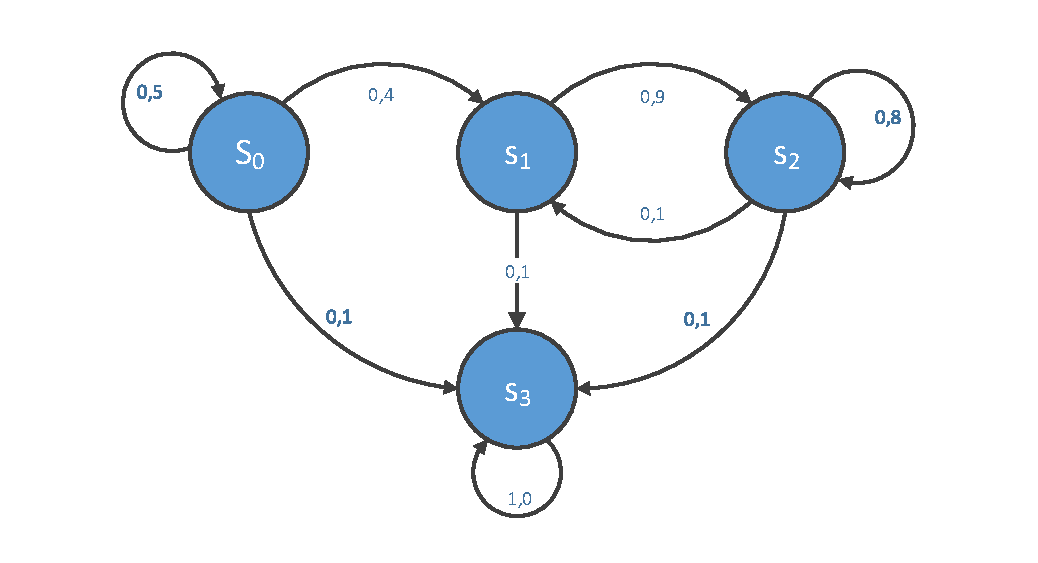
\includegraphics[trim=10px 10px 10px 10px, clip, width=0.8\columnwidth]{figures/rl/markov_chain.pdf}
  \end{center}
  
  %\vspace*{-6pt}
  \caption[An Markov Chain Example]{An example for a Markov chain. Suppose we start in $s_0$. There is a 50\% chance of staying in that state, a 40\% chance of transitioning to $s_1$ and a 10\% chance of transitioning to $s_3$. No matter how long it alternates between $s_0$, $s_1$ or $s_2$ at some point it will enter $s_3$ and remain there forever, because $s_3$ has a 100\% chance of transitioning to itself.}
  \label{fig:MarkovChain}
  %\vspace*{-12pt}
\end{figure}


Markov decision processes extend the idea of Markov chains with an active agent. At each step, the agent can choose from a set of actions and the state transition probability depends on the chosen action. Additionally each state transition may return some reward. The agents goal is to find a policy which maximizes the total reward over time. We extended our example from Figure \ref{fig:MarkovChain} with actions and rewards in Figure \ref{fig:MDP}. Like for Markov Chains, MDPs transition probabilities must only depend on the current state $s$ and the chosen action.

\begin{figure}[ht]
  
  \begin{center}
      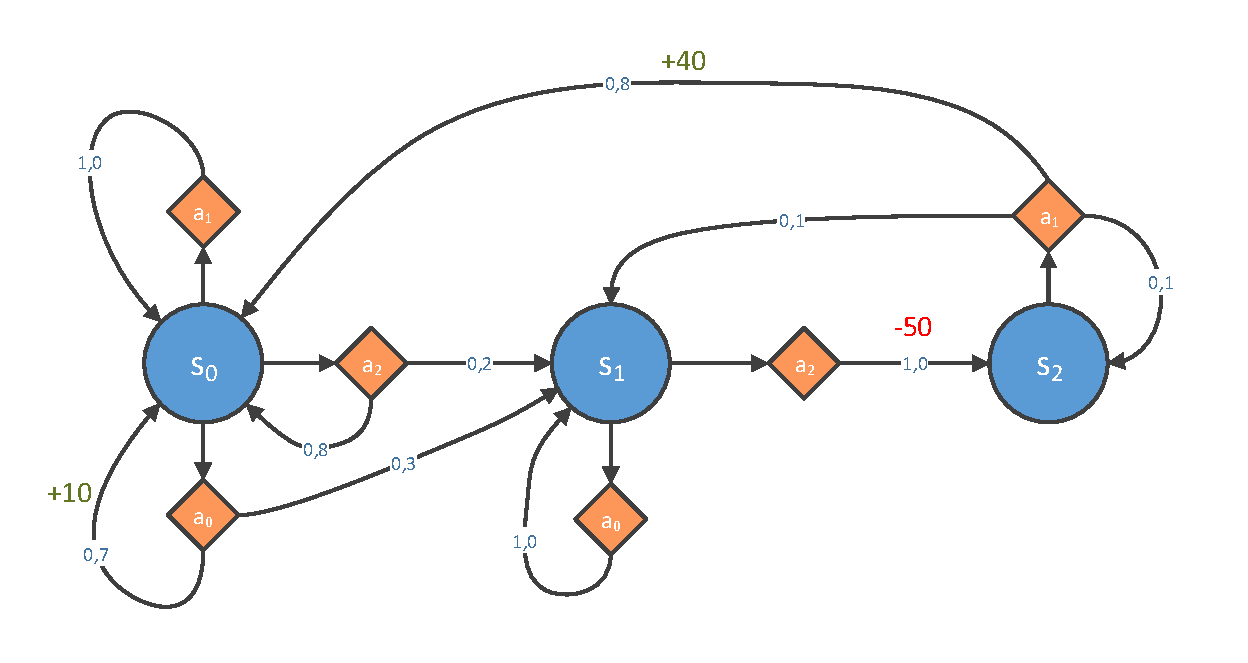
\includegraphics[trim=10px 10px 10px 10px, clip, width=0.9\columnwidth]{figures/rl/markov_decision_process.pdf}
  \end{center}
  
  %\vspace*{-6pt}
  \caption[An Example for the Markov Decision Process Example]{An example for the Markov decision process (recreated from \cite{handson2019geron}). Again we start in $s_0$ and the agent can choose from the actions $a_0$, $a_1$ or $a_2$. Choosing $a_0$ will give it a reward of $+10$. With a probability of 70\% the agent will be staying in $s_0$ and with a probability of 30\% it will transition to $s_1$. So the agent can likely repeat action $a_0$ in $s_0$ multiple times, but will at some point transition to $s_1$. In $s_1$ it now only has the options to stay there or go through a $-50$ penalty, which might even be repeated. The question is which strategy leads statistically to the most reward? Maybe choosing $a_0$ until we end up in $s_1$ and then never leave $s_1$ by always choosing $a_0$? Or going through the penalty and then collecting positive reward again? We will take a detailed look how we can solve this problem in the introduction of Section \ref{sec:ValueMethods}.}
  \label{fig:MDP}
  %\vspace*{-12pt}
\end{figure}

When modeling a RL problem as MDP we have a problem: The Markov assumption. If we look at the probability of our states, we would normally consider that at step $t$ the next state $s_{t+1}$ is sampled from a probability distribution depending on all the previous states and actions.

\[s_{t+1} \sim P\left(s_{t+1}|(s_0, a_0), (s_1, a_1), \dots, (s_t, a_t)\right)\]

 This sound logical, since the agent might also work with a stochastic policy which picks actions partially at random. Also reaching a state might influence other states or their transition probabilities. This not only violates the Markov assumption, it makes it extremely hard for an agent to approximate that underlying transition function for $P$ to make reasonable decisions in our environment. Therefore we need to simplify our model to:  

 \[s_{t+1} \sim P(s_{t+1}|(s_t, a_t)\]

This form sacrifices some freedom, but is still powerful enough and leads to much simpler transition functions which can be learned much easier. Despite the fact that a state transitions now only can depend on the last state and action, we can look at it from a different angle to reintroduce some of our freedom again. Any state can be defined to include any necessary information and there can be an unlimited (but fixed) number of states in our model. For example imagine a game where you if you win round one get a slight bonus for round two. Then the states and their transitions of round two would depend on round one. What we can do is introduce two completely new sets of states for round two where one set has the information attached that we won and one that we lost. This way the states for round two do not depend on round one, we just have more states and transitions. Using this trick helps us model many complex environments as MDP.

Agents in RL only decide upon an observation and not on the internal state of the environment. Also they normally do not know all states or their transition probabilities in the MDP. Therefore we often talk about a \textit{partially observable MDP} (\textit{POMDP}) in the context of reinforcement learning.

\paragraph{Reward and Return.} %TODO: Image/Example for discounted reward.
in our model, the agent may receive some reward after or during each state transition: $r_t = R(s_t, a_t, s_{t+1})$. The agents goal is to maximize the total sum of expected reward, but - as we discussed earlier - it is complicated to know which action action was responsible for which reward. If we look back at the example from Figure \ref{fig:MDP}: How much reward do we generate by choosing $a_0$ in $s_0$? We have a probability of generating $+10$ reward, but we might also get no reward and end up in $s_1$. How much reward we are able to generate once we ended up in $s_1$ is also unclear.

To build a better connection between actions and reward, instead of associating rewards directly with the action which was chosen right before the reward was returned, we calculate the return $R$. The return is defined as a sum of future rewards, which we are able to achieve from the current state when choosing a certain action. Depending on the task, this sum can be formulated in different ways. This way an action which results in negative reward can actually be actually seen as a good action, if it generates much more positive reward in the future and the other way around.

Since most of the time, the current action is not directly associated with every future reward, we look at so-called \textit{discounted rewards}. We call this reward the \textit{finite-horizon discounted return} with a discount factor $\gamma \in [0, 1]$:

\[R(\tau) = \sum_{t=0}^T \gamma^t r_t\]

The discount factor is an important variable which controls how much we value future rewards and needs individual tuning for every environment. Small values for $\gamma$ lead to more "shortsighted" actions - with the extreme case $\gamma = 0$ valuing just the initial (next) reward. The other extreme case with $\gamma = 1$ just means there is no discount and which therefore is called the \textit{finite-horizon undiscounted return}: 
\[R(\tau) = \sum_{t=0}^T r_t\] 

Sometimes we are also dealing with environments with infinite episode lengths. If $T$ is unbounded we talk about an \textit{infinite-horizon discounted return}. In this case $\gamma$ needs to be smaller than 1 to bound our future rewards.

\paragraph{The RL Problem.}
Before we look at the first RL algorithm, we want to give a mathematical definition for the reinforcement learning problem itself. If the goal of the agent is to maximize the total reward from the environment, RL algorithms will select a policy which at each step maximizes the \textit{expected return} by choosing an optimal action $a^*$ under observation $o$. Depending on the chosen discount factor this return will depend more or less on future rewards.

Lets look at an example, where both the environment transitions and the policy are stochastic. The probability for a trajectory with $T$ steps is: 

\[P(\tau|\pi)=\rho(s_0)\prod_{t=0}^{T-1}P(s_{t+1}|s_t, a_t)\pi(a_t|o_t)\]

We denote the \textit{expected return} for the current policy $\pi$ by $J(\pi)$. For some trajectory $\tau$ this return is equal to:

\[J(\pi) = \int_\tau P(\tau|\pi)R(\tau) = E_{\tau\sim\pi}\left[R(\tau) \right]\]

In case of finite-horizon discounted return we get 

\[J(\pi) =  E_{\tau\sim\pi}\left[R(\tau) \right] = E_\tau\left[\sum_{t=0}^T \gamma^t r_t\right]\]

Given this definition for expected return, we can formulate the problem of reinforcement learning as the problem of computing an optimal policy $\pi^*$ which maximizes expected return over a trajectory:
\[\pi^*=\argmax_\pi J(\pi)\]

\section{Value-Based Methods} \label{sec:ValueMethods}
In this section we want to take a look at the first family of reinforcement learning algorithms: The value based methods. We begin by looking at a technique called \textit{value iteration}, which will allow us to calculate state values in a MDP, in Section \ref{ssec:Value_Iteration}. We will then continue to explore how this technique can be used to learn state-action values (called $Q$-values) from a partially unknown MDP in Section \ref{ssec:TDLearning}, which leads directly to our basic value-based RL algorithms \textit{SARSA} (Section \ref{ssec:SARSA}) and the \textit{Q-Learning algorithm} (Section \ref{ssec:Q_Learning}). Finally we will combine the Q-Learning algorithm with neural networks into Deep Q-Learning in Section \ref{ssec:DeepQLearning} and look at a number of Deep Q-Learning extensions in Section \ref{ssec:DQNExtensions}. 

\subsection{Value Iteration} \label{ssec:Value_Iteration}

In Section \ref{sec:concepts} we already saw that we can express our RL problem as a Markov decision process. Bellman did not only create the model, but also found a way to estimate the optimal state value of any state in an MDP. This state value is calculated by looking at all discounted future rewards an agent can expect if it currently is in state $s$ and then acts optimally for all future transitions. In the Equation \ref{eq:Optimal_State_Value} $T(s, a, s')$ denotes the transition probability for state $s'$ if the agent is in state $s$ and chooses action $a$.  

\begin{equation} \label{eq:Optimal_State_Value}
V^*(s) = \max_a \sum_{s'} T(s, a, s')\left[ R(s, a, s') + \gamma V^*(s')\right]
\end{equation}

We can see that the equation is recursive, since we calculate the value for the current state by adding the transition reward to the state values of the possible next states weighted by their transition probability. We also discount the value of the next state by our discount factor $\gamma$. Bellman described a simple a algorithm called \textit{value iteration} which calculates this optimal state value \cite{bellman1957markovian}. It works by initializing all state values to zero and iteratively calculating

\[V_{k+1}(s) = \max_a \sum_{s'} T(s, a, s')\left[ R(s, a, s') + \gamma V_k(s')\right]\]

Fortunately this algorithm is guaranteed to converge. Depending on how interested we are in exact values, we can always cancel the iteration early and look at the intermediate results in the $k$th iteration. The problem is knowing the current value of the state we are in does not tell us which action we should take next. The equation is not suited to derive a policy from it. Luckily Bellman also found, that it is easy to reformulate the equation to calculate $Q^*(s, a)$ which is the optimal value we can expect if we choose action $a$ and then always act optimally. We define this value in Equation \ref{eq:Optimal_Q_Value}. This value can again be calculated by value iteration, as can be seen in Equation \ref{eq:Q_Value_Iteration}:

\begin{align}
  Q^*(s, a) &= \sum_{s'} T(s, a, s')\left[ R(s, a, s') + \gamma \max_{a'} Q^*(s', a')\right] \label{eq:Optimal_Q_Value}\\
  Q_{k+1}(s, a) &= \sum_{s'} T(s, a, s')\left[ R(s, a, s') + \gamma \max_{a'} Q_k(s', a')\right] \label{eq:Q_Value_Iteration}
\end{align}

With the optimal Q-value at hand, defining the optimal policy is as easy as defining $\pi^*(s) = \argmax_a Q^*(s, a)$. So are we at the end? Do we have the ultimate tool for every RL problem? Sadly the answer is no, because while we could calculate our policy exactly in that way, we do not have the information to do so. In a real RL scenario we do not know the underlying MDP - we have to discover all states, rewards and transition probabilities first. 

\subsection{Temporal Difference Learning} \label{ssec:TDLearning}
The basic algorithm used for Q-Learning is called \textit{Temporal Difference Learning} (TD Learning). This algorithm is very similar to the value iteration method and also connected to the stochastic gradient decent algorithm. The unknown MDP is usually explored using a stochastic policy. In the easiest case this policy is just sampling a random action from our action space for each state. We then iteratively improve our state estimation by calculating:

\[V_{k+1}(s) \leftarrow (1-\alpha) V_k(s) + \alpha (r + \gamma V_k(s')) \]

In this equation $\alpha$ is a parameter for the learning rate in the interval $[0, 1]$. The term is usually rewritten to emphasize that we change our estimation by having an error term:

\begin{equation*}
  V_{k+1}(s) \leftarrow V_k(s) + \alpha \underbrace{(\underbrace{r + \gamma V_k(s')}_\text{TD Target} - V_k(s))}_\text{TD Error}
\end{equation*}

Again the basic TD learning method is formulated for the value function and we have to reformulate it for Q-Value estimation. Also we now have to decide how we explore the environment. Depending on our choices we end up with either \textit{SARSA} or the classical \textit{Q-Learning} algorithm.

\subsection{SARSA} \label{ssec:SARSA}
We are finally at the point where we can look at the first reinforcement learning algorithm: SARSA, which was proposed by Rummery and Niranjan in 1994 \cite{rummery1994line}. SARSA uses the same method or values to sample actions and learn from them, therefore SARSA is a so called \textit{on-policy} learning algorithm. We will talk about the difference to \textit{off-policy} algorithms in a moment when we come to classical Q-learning.

The name SARSA was not originally proposed, but is widely used and comes from the parameters that are needed to make a single update step. The agent which currently is in state $s$ takes action $a$ and gets return $r$. It then samples a new action based on $s'$ from its policy (which is a stochastic policy) and chooses action $a'$, combined we get  state-action-reward-state-action $(s, a, r, s', a')$ - the origin of the name.

SARSA uses the TD-learning method to update its Q-value estimation:

\[Q_{t+1}(s, a) \leftarrow Q_t(s, a) + \alpha (r + \gamma Q(s', a') - Q(s, a))\]

For each state-action pair, SARSA calculates a running average of the rewards $r$ combined with the sum of expected discounted future reward. This way SARSA is able to estimate optimal Q-values for every state-action pair given enough iterations. We included a sketch of this procedure in Algorithm \ref{alg:SARSA}.

\begin{algorithm}[ht]
  %\KwData{}
  \KwResult{Estimated Q-Values for $Q(s, a)$}
  Initialize $Q(s, a)$ for $\forall s \in S$ and $\forall a \in A$ randomly. $Q(terminal, \cdot) = 0$ \;
 \ForEach{episode}  {
   $s \sim \rho(\cdot)$ \tcp*[f]{Sample initial state}\;
   Choose $a$ from $s$ using a policy derived from $Q$ (e.g. $\epsilon$-greedy) \;
   
   \ForEach{step in episode}  {
     Take action $a$, observe $r$, $s'$ \;
     Choose $a'$ from $s'$ using policy derived from $Q$ (e.g. $\epsilon$-greedy) \;
     $Q(s, a) \leftarrow Q(s, a) + \alpha (r + \gamma Q(s', a') - Q(s, a))$ \;
     $s \leftarrow s'$, $a \leftarrow a'$ \;
   }
 }
  \caption[The SARSA Algorithm]{SARSA Algorithm for On-Policy TD Q-Value Estimation (adapted from \cite{sutton2018reinforcement})}\label{alg:SARSA}
 \end{algorithm}

We just mentioned that actions are sampled from our policy, but what exactly is our policy? To this point we only talked about the calculation of Q-values. If we already calculated all our Q-values, it seems to be clear that the best policy would be to always choose the action for the current state with the highest Q-value. The problem when learning is we do not know the best Q-value for each state yet. At this point we come back to a problem we discussed in Section \ref{ssec:rlidea}: The balance between exploration and exploitation. We need a policy which explores the environment in a way that allows us to calculate Q-values for every state. Therefore we need a policy which will visit each state - not only once multiple times to get sufficient good Q-Value estimations.

If we strictly follow an exploration policy which already exploits our estimated Q-values we will likely end up only exploring a fraction of all states and get stuck in a local optimum. So instead we will use a stochastic policy in SARSA. If we take the other extreme and use a completely random policy the agent will always be able to visit all states eventually, but may need extremely long to do so. Therefore the most commonly used policy is an $\epsilon$-greedy policy, which combines a stochastic exploration with an estimated Q-Value exploitation. In this policy at each step we have the probability $\epsilon$ for which we take a random action and with probability $(1 - \epsilon)$ we choose the action with the highest Q-value. This way we will explore the environment enough, but still direct learning to be more focused on promising states. Often times $\epsilon$ will not be set to a fixed value. Instead $\epsilon$ will be a function over the course of the training process, starting with high values (mostly random actions) and then gradually decreasing over time. 

\subsection{Q-Learning} \label{ssec:Q_Learning}
Q-Learning actually predates SARSA, and was developed in 1992 by Chris Watkins \cite{watkins1992q}. Today, Q-Learning is one of the most popular methods in RL. As for SARSA, in Q-Learning we estimate state-action values with the TD learning algorithm. The difference is that we are now dealing with an off-policy algorithm. This means that the policy that is being trained is not (or only partially) executed during the training process. You can find the procedure in Algorithm \ref{alg:QLearning}.  

\begin{algorithm}[ht]
  %\KwData{}
  \KwResult{Estimated Q-Values for $Q(s, a)$}
  Initialize $Q(s, a)$ for $\forall s \in S$ and $\forall a \in A$ randomly. $Q(terminal, \cdot) = 0$ \;
 \ForEach{episode}  {
   $s \sim \rho(\cdot)$ \tcp*[f]{Sample initial state}\;
   \ForEach{step in episode}  {
    Choose $a$ from $s$ using exploration policy (e.g. random or $\epsilon$-greedy) \;
     Take action $a$, observe $r$, $s'$ \;
     $Q(s, a) \leftarrow Q(s, a) + \alpha (r + \gamma\max_{a'} Q(s', a') - Q(s, a))$ \;
     $s \leftarrow s'$\;
   }
 }
  \caption[The Q-Learning Algorithm]{Basic Q-Learning Algorithm for Off-Policy TD Q-Value Estimation (adapted from \cite{sutton2018reinforcement})}\label{alg:QLearning}
 \end{algorithm}

We can see that while both algorithms are pretty similar, there are a few differences. Instead of using a stochastic policy and using that policy to choose an action $a$ \textbf{and} for estimating the future reward (the $Q$ value), we now only use a stochastic policy to sample $a$ and then always use a greedy policy. This can be interpreted in a way that the algorithm considers its estimated Q-Values to be optimal even if they are not. Therefore our update rule becomes: 
\[Q_{t+1}(s, a) \leftarrow Q_t(s, a) + \alpha (r + \gamma\max_{a'} Q_t(s', a') - Q_t(s, a))\]

Q-Learning even works if the exploration policy is completely random, even though $\epsilon$-greedy type strategies are often faster. So again, are we finished yet? If Q-Learning is able to calculate optimal Q-Values and thus provides us with an optimal policy we can now always use Q-Learning, right? The problem is while Q-Learning is able to calculate the optimal Q-values, it may need a very long time to do so. And since Q-Learning uses a table for every state that is possible in our environment, problem size exponentially increases for many environments.

If you think of the simple game of Tic-Tac-Toe we have 9 boxes where each player may set his mark, so end up with $2*2^9+9=1033$ possible states. For such a simple game thats a surprisingly high number. And it gets even worse if we look at games which allow for even more combinations. If we take the computer game classic \textit{Pac-Man}, we can see every coin the player can capture as a single state. With around 100 coins we are already at $2^{100} \approx 10^{30}$ states. And the coins are not the only thing which may change state in that game. With traditional Q-Learning we would not only need ages to explore all states, we would also end up with a huge table of state-action values which might not fit in our memory.

\subsection{Deep Q-Learning} \label{ssec:DeepQLearning}
When we are dealing with a huge number of states, we might want to sacrifice some of the accuracy of our predictions for the sake of actually being able to compute these predictions in a reasonable time. To achieve this instead of computing a table containing a value approximation for every state-action pair we will compute a (nonlinear) function which approximates these values. Ideally this function should have an amount of parameters which is much smaller than the number of possible states. We denote this function as $Q_\theta(s, a)$. As we know from Chapter TODO artificial neural networks are highly nonlinear parameterizable functions. This means we can use neural networks to approximate our Q-values. In 2013, the DeepMind team showed, that using deep neural networks for Q-value approximation has a stellar performance on playing multiple games from the Atari 2600 game console \cite{mnih2013playing}. Their work also proved, that it is not necessary to handcraft features for the neural network. Instead a raw image from the game is sufficient and even results in better performance.

We call a deep neural network that is used for Q-Value estimation a \textit{Deep Q-Network} (DQN) and indicate that our Q-value is estimated by subscripting our Q-function with $\theta$ denoting the parameters of our neural network. Using a DQN for approximate Q-Learning is called \textit{Deep Q-Learning}.

To train a neural network we still need a key element: A loss function. The loss function should represent how much the value calculated by the neural network deviates from the target value. Similar to how we calculated our updates in classical Q-Learning we treat our estimation as if we already know the best Q-Values. Our target Q-Value then is 

\[Q_{target}(s, a) = r + \gamma \cdot \max_{a'}Q_\theta(s', a')\]

Using a common metric like the mean square error we can calculate the difference between the estimated Q-Value of our network and the target Q-Value to get a loss function.

\[\mathcal{L} = (Q(s, a) - Q_{target}(s, a))^2\]

\begin{figure}[t]
  
  \begin{center}
      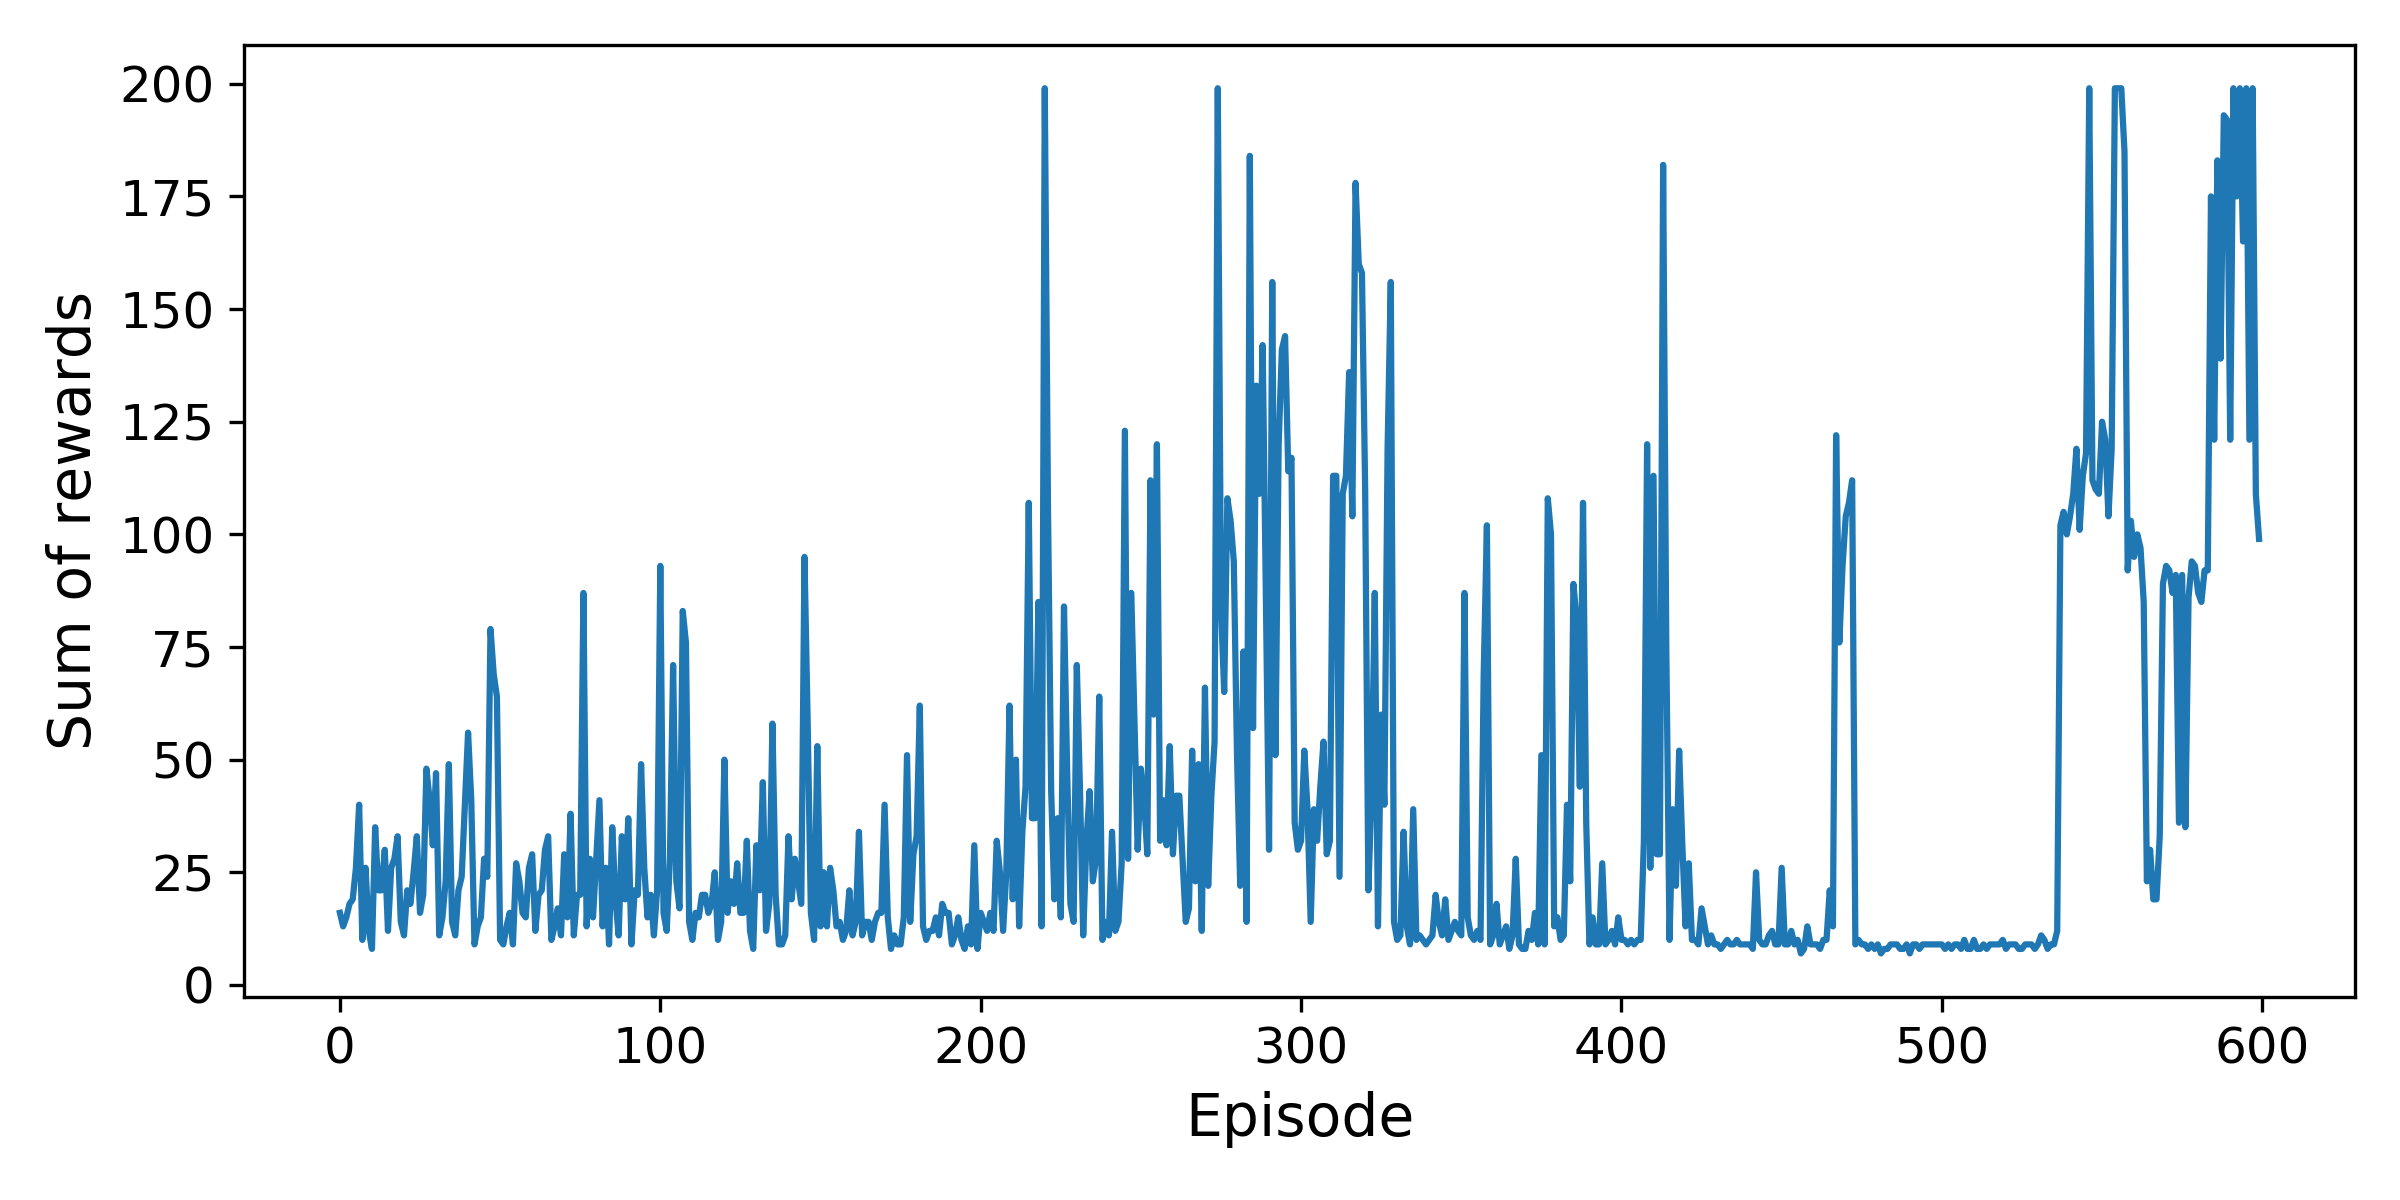
\includegraphics[clip, width=0.8\columnwidth]{figures/rl/dqn_cart_pole_plot.png}
  \end{center}
  
  %\vspace*{-6pt}
  \caption[Learning Curve for Deep Q-Learning on CartPole]{Learning Curve for basic Deep Q-Learning only with simple experience replay on the CartPole environment.}
  \label{fig:learning_curve_dqn}
  %\vspace*{-12pt}
\end{figure}

By defining a loss function we can train our neural network in the same fashion as in supervised learning using the well-known stochastic gradient decent algorithm. This will need thousands or even millions of updates to converge - if it ever does. Deep Q-Learning in its basic form suffers from a lot of problems which results in a DQN learning either slowly, not at all, or suffering from a problem called \textit{catastrophic forgetting}. Figure \ref{fig:learning_curve_dqn} shows the reward over time when solving the CartPole environment. As we can see the agent does not learn anything for 300 episodes, then suddenly achieves the maximum possible reward of 200 and then seems to forget what it has learned. This process then alternates back and forth. Problems like this emerge from a number of different problems:
 \begin{enumerate}
  \item The SGD algorithm assumes that we have data that is \textit{independent and identically distributed} (i.i.d), but our training data is neither independent nor identically distributed. Our samples are generated in episodes which typically make state transitions between states which have a lot in common (e.g. two adjacent frames in a game). Also the distribution of our data is not similar to the distribution the data would have if it has been sampled from an optimal policy. 
  \item We learn from data generated by our current policy (or from a partially random policy in case of $\epsilon$-greedy), which will create samples which are highly correlated. Additionally we use the same model we created our samples with to set our target value and calculate our loss. This may result in a feedback loop which makes training unstable.
  \item In training, the agent will likely overestimate Q-Values. This is due to the nature of the update process. In each step, the target model will select the highest Q-Value, but all Q-Values are estimated. Think of a situation in which each action for a given state has the same Q-Value. An approximation will never be exact, so some of the Q-Values will be slightly higher and some will be slightly lower. When selecting the next Q-Value we do not go for an average we select the highest. Thus we are always prone to overestimation.
 \end{enumerate}

 All these problems combined lead to a very unstable learning process. Fortunately over the years many extensions were developed to reduce their impact dramatically.

\subsection{DQN Extensions} \label{ssec:DQNExtensions}
In this section we want to give a brief overview over techniques that were developed to make Deep Q-Learning more stable. 

\paragraph{Experience Replay.}
At first we want to focus on breaking the correlation between the samples. If we always train from a single episode all our training data will be highly correlated and states will look almost identical. To overcome this instead of learning directly from the trajectory generated by a single episode we introduce a \textit{replay buffer}. After playing an episode we draw random samples from our buffer and learn from them. This will break up the correlation between samples and also reduces the danger of forgetting already learned behavior. On the negative side it introduces new hyperparameters with the size of the replay buffer and the number of samples we want to draw for learning, which are both dependent on the task we are trying to solve. 

\paragraph{Prioritized Experience Replay.}
Lets take the idea of the replay buffer to the next level: Since not all of our samples might be equally important for the learning process, it would be a good idea to replay interesting samples more often than others. This procedure is called \textit{importance sampling} (IS) or \textit{prioritized experience replay} (PIR) and was developed in 2015 by the DeepMind Team \cite{schaul2015prioritized}. The question is what are interesting samples? Schaul et al. proposed to use the TD error term $\delta = r+\gamma V_k(s') - V_k(s)$ (see Section \ref{ssec:TDLearning}) as an indication of a sample being interesting. This makes sense if you think about what a large error means for our algorithm: If we estimated a state value wrong, it is equal to saying we are surprised by the result of the state value. Thus the sample is interesting.

In our replay buffer we now assign a priority to each sample, depending on how large the TD error is. We set this priority to a high value for the first time, to ensure that the sample will be sampled at least one time and update the sample priority each time it is sampled to $p = |\delta| + \epsilon$ with $\epsilon$ being a small positive constant to ensure each sample has a non-zero probability of being drawn. A single sample then has the probability of 

\[P(i) = \frac{p_i^\alpha}{\sum_k p_k^\alpha}\]

The exponent $\alpha \in [0, 1]$ is a new hyperparameter which defines how much weight is given to importance sampling with $\alpha = 0$ being standard uniform experience replay.

With some samples being sampled more often than others we again violate our goal of learning uniformly on samples from the target distribution that would be observed if the agent would behave optimally. Without a compensation for this bias, our agent would overfit on those high priority samples. To compensate, we downweight more important samples in training by 

\[w_i = \left(\frac{1}{N} \cdot \frac{1}{P(i)}\right)^\beta\]

where $\beta \in [0, 1]$ is another hyperparameter which controls how much we want to compensate (0 means no compensation). PIR has shown to vastly improve convergence speed and overall performance of Deep Q-Learning, but also introduces two additional hyperparameters which need to be tuned.

\paragraph{Target Networks.}
The next extension aims at improving training stability and reducing the problem of a feedback loop. Since we use the same network to generate samples and to calculate the target Q-Values, situations where training is unstable, diverges or oscillates are very likely. This can be broken up by separating the prediction when generating samples from the calculation of the target values. This is done by working on two similar - but not identical - copies of the same network. We call one of them the \textit{online model} and one the \textit{target model}. The online model will interact with the environment and get updated in the regular update step, while the target model only makes the predictions for the target Q-Value. Every once in a while we copy the weights of the online model to the target model.

\paragraph{Double DQN.}
Next up we want to reduce Q-Value overestimation. This can be done by improving the usage of our target network: Instead of always selecting the action with the highest Q-Value for the Q-target in the update step, we select the action with the highest Q-Value from the online model, and then use the Q-Value estimation for that action from the target DQN. This method was also developed by DeepMind and is called \textit{Double DQN} (DDQN) \cite{van2016deep}.

\paragraph{Dueling DQN.}
Another technique which aims at stabilizing learning is called Duelling DQN \cite{wang2015dueling} (not to be confused with Double DQN). Duelling DQN changes the architecture of the DQN to not compute Q-Values directly, but rather compute two values: The state value $V(s)$ and the so-called \textit{advantage} $A(s, a)$. The advantage expresses how good it is to take an action $a$ in state $s$ in comparison with every other action. If we look at the advantage for an optimal policy $A^*(s, a)$, the best action $a^*$ will have an advantage of 0. We can express the Q-Value as $Q(s, a) = V(s) + A(s, a)$. Computing multiple values which are connected to the same task proves to be beneficial for the training of neural networks and greatly stabilizes training. Therefore we extend our neural network to compute both $V(s)$ and $A(s, a)$ for every action.  %TODO: Source? 

\paragraph{Even more extensions.}
We already discussed a lot of important extensions for Deep Q-Learning, but there are even more. Update steps can be combined into multi-step learning which further stabilizes the training process \cite{sutton1988learning}. Instead of learning to approximate the returns we can also learn to approximate the distribution of returns \cite{bellemare2017distributional}. Like for every neural network the introduction of noise often results in more robust predictions. Additionally the introduction of noise is beneficial in RL because it improves exploration \cite{fortunato2017noisy, plappert2017parameter}.

Most of the techniques to improve Deep Q-Learning that were discussed can also be used in conjunction. In 2018 the DeepMind team created an agent which they called \textit{Rainbow} and which was able to outperform all standalone techniques on the Atari 2600 benchmark \cite{hessel2018rainbow}. Even though this proves that the combination of these extensions can be beneficial, the introduction of several new hyperparameters requires careful fine-tuning which might take a lot of time even with modern hyperparametersearch algorithms. %TODO: Make figure for learning with extensions.

\section{Policy Gradient Methods} \label{sec:PGMethods}
We already saw, that Q-Learning (with its extensions) is a very powerful tool to solve RL problems. Nevertheless we also saw that Q-Learning suffers from a lot of problems and with all its extensions is hard to parameterize correctly. Also we are not able to solve RL problems with continuous action spaces, since there would be an infinite number of actions to choose from. Therefore we need an alternative way to deal with reinforcement learning problems.

Let us look at what we are doing in Q-Learning: We estimate values $Q_\theta(s, a)$ and then derive an optimal policy by $\pi^*(s) \approx \argmax_a Q_\theta(s, a)$. So we are only indirectly learning an optimal policy. While the Q-Value might be interesting, at the end we do not need to know how much better an action is compared to others. We are only interested in acting optimally. So instead of estimating Q-Values and then deriving an optimal policy, we want to directly learn the optimal policy. This is the idea behind \textit{Policy Gradient} (PG) methods which aim at iteratively computing an optimal policy by using gradients in policy space.

We will only look into a single member of this family in Section \ref{ssec:REINFORCE}: The REINFORCE algorithm. This is because the PG-methods quickly involved into combined methods which take ideas from both Q-Learning and REINFORCE and combine them to achieve even better results.

\subsection{REINFORCE} \label{ssec:REINFORCE}
The REINFORCE algorithm was invented in 1992 by Ronald Williams \cite{williams1992simple}. The algorithm computes a policy which produces action probabilities directly from states. Like in Deep Q-Learning we use a neural network as our policy, which directly outputs probabilities for actions in the discrete case and values for actions in a continuous setting. The name REINFORCE originates from the simple idea of positively reinforcing actions which proved to yield good results while discouraging actions which yield bad results. This reinforcement is done iteratively in small steps by application of policy gradients.

So let us begin by defining what a policy gradient should be. Remember our definition for expected return $J(\pi)$ from Section \ref{ssec:RLMDP}. We extend our notion to also include the parameters of our neural network. We can then define our goal as finding the parameters for our network which maximize the expected return:  

\begin{equation} \label{eq:PGObjective}
  \max_\theta J(\pi_\theta) =  E_{\tau\sim\pi_\theta}\left[R(\tau) \right]
\end{equation}

So how do we maximize the expected return and find the correct parameters? If we look at our objective $J(\pi_\theta)$ we can think of it as an abstract hypersurface for which we are trying to find a maximum. The dimensions of the surface are given by the network parameters $\theta$ and the "height" is our return. To gradually improve our policy, we are using gradient ascent (which is the same as gradient descent, but now we are using the gradients to find a maximum) for $J(\pi_\theta)$

\[\theta \leftarrow \theta + \alpha \nabla_\theta J(\pi_\theta)\]

The gradient $\nabla_\theta J(\pi_\theta)$ is our \textit{policy gradient} and $\alpha$ is our learning rate. But at this point we have a problem: If we look at Equation \ref{eq:PGObjective} we can see, that $\nabla_\theta J(\pi_\theta)$ is not differentiable with respect to $\theta$ because $R(\tau)$ is not dependent on $\theta$. Also the function $R(\tau)$ itself is unknown. Since the expected reward is directly dependent on the decisions of the current policy, it is possible to rewrite the equation into a form that is differentiable:

\begin{equation} \label{eq:PGEstimation}
  \nabla_\theta J(\pi_\theta) = E_{\tau \sim \pi_\theta} \left[\sum^T_{t=0}R_t(\tau) \nabla_\theta \log \pi_\theta(a_t|s_t)\right]
\end{equation}

We omit the proof here, but it can be found in \cite{foundations2019graesser}. Now that we have a gradient we can optimize, we can take a look at the final REINFORCE algorithm shown in Algorithm \ref{alg:REINFORCE}.

\begin{algorithm}[ht]
  \KwData{Learning Rate $\alpha$}
  \KwResult{Optimal policy parameters $\theta$}
  Initialize weights $\theta$ of policy network $\pi_\theta$ randomly. \;
 \ForEach{episode}  {
   Sample trajectory $\tau = ((s_0, a_0, r_0), \dots, (s_T, a_T, r_T))$ with $\pi_\theta$ from the environment \;
   $\nabla_\theta J(\pi_\theta) \leftarrow 0$ \;
   \For{$t=0, \dots, T$}  {
    $R_t(\tau) = \sum^T_{t'=t} \gamma^{t'-t}r_t$ \;
    $\nabla_\theta J(\pi_\theta) = \nabla_\theta J(\pi_\theta) + R_t(\tau)\nabla_\theta \log \pi_\theta(a_t|s_t)$ \;
   }
  $\theta \leftarrow \theta + \alpha \nabla_\theta J(\pi_\theta)$
 }
  \caption[The REINFORCE Algorithm]{The REINFORCE Algorithm (adapted from \cite{foundations2019graesser})}\label{alg:REINFORCE}
 \end{algorithm}

After initializing the policy, we sample trajectories $\tau$ from the \textit{current} policy. These trajectories are then used to \textit{estimate} $\nabla_\theta J(\pi_\theta)$. The estimations are calculated by collecting individual gradients for each sample of the current episode and calculating the gradient according to Equation \ref{eq:PGEstimation} in Line 7. Note that this estimation of $\nabla_\theta J(\pi_\theta)$ may not be exact and lead to problems in the training process. 

Once we have estimated the gradients, they are applied in a single gradient ascent step. This is usually done by an advanced optimizer like Adam (see Section \ref{sec:NNChallenges}), but we always use vanilla gradient ascent for clarity. Because we estimate the gradients for our policy, by sampling data from our policy, REINFORCE is an on-policy algorithm. This also means that we have to discard our samples after each update - they cannot be used to estimate gradients for the next update step. Because this is true for all policy-based methods, they are usually called sample inefficient. This means that algorithms which estimate policy gradients need a high number of environment interactions for their training process, which could be a problem if the environment is computationally expensive or we are dealing with real world interactions.

Note that in REINFORCE we do not need a dedicated exploration policy. Instead, exploration is now build into our network, which directly outputs action probabilities for a given state. We then use these probabilities to sample an action according to the given probability distribution. In comparison with Q-Value estimation with all its extensions, we now have a much simpler way of computing our optimal policy. There is no need for a replay buffer or a target network copy. We also extended our possibilities into continuous actions and are now able to model stochastic environments. Unfortunately there are also downsides to policy gradient methods: Because we are dealing with relatively small sample estimations, our estimations may be unstable and cause a lot of variance in our gradients. Samples from a single trajectory are also highly correlated. Because the exploration now completely depends on the current agent, policy-based learning is prone to getting stuck in local optima. We will look at ideas of how to overcome all these problems in Section \ref{ssec:ImprovingPG} and Section \ref{sec:CombinedMethods}.

\subsection{REINFORCE Improvements} \label{ssec:ImprovingPG}
We already talked a little bit about problems with the REINFORCE algorithm and policy gradient methods in general in Section \ref{ssec:REINFORCE}. We now want to take a detailed look at how we can improve policy gradient methods and overcome or at least reduce the impact of these problems.

\paragraph{Learning from Steps.}
Let us go back and take another look at Algorithm \ref{alg:REINFORCE}. The algorithm is written in a way that we need to complete a full episode, before we get into training. This might become a problem if episodes are really long or even never end at all. With long episodes it will take a very long time before we can actually learn anything and we have to discard all that data immediately after. Therefore it would be beneficial, if it was possible to learn from a single or just a few steps of environment interaction. 

Currently we are computing our gradient with a sample estimate over the entire episode. If you look at Equation \ref{eq:PGEstimation} we can actually substitute $R_t(\tau)$ by $Q_\theta(s_t, a_t)$. This means we do not actually need a full episode to train our network, we only need an estimate for the expected return according to our policy. The problem is unlike with DQN we now only have a network which can tell us the optimal action. We do not know the Q-Values anymore. There are two possible solutions for this problem:

\begin{enumerate}
  \item \textbf{Unrolling.} First let us reformulate the equation again and substitute $R_t(\tau)$ with $r_t + \gamma V_\theta(s')$ (which is equal to $Q_\theta(s_t, a_t)$). Since $V_\theta(s)$ is recursive, we can see, that future state values get exponentially discounted by $\gamma$. Since the impact of future state values on the current state value gets exponetially smaller, ff $\gamma$ is small enough we can ignore recursions after a certain depth. This means we can approximate $V_\theta(s)$ by unrolling for a fixed number of steps $N$ in the future. This way we only need a trajectory which is at least $N+1$ steps long to calculate an update for the first step. 
  \item \textbf{Value Networks.} We can extend our neural network to also output the state value for the current state. This is done in most of the combined algorithms we will look at in Section \ref{sec:CombinedMethods}.  
\end{enumerate}

\paragraph{High Gradient Variance.}
If we sample a trajectory from the environment using our current policy, the return we get for that episode may include a significant amount of variance. This variance comes from multiple factors. Since we start in a randomly sampled state, choose our actions at random from the action probability distribution of our policy and (in some environments) need to deal with stochastic state transitions, two adjacent episodes might result a totally different reward. Take a card game for example where we get an initial random set of cards drawn to our hand. If the cards are good, we are way more likely to win the round and get much reward, but that does not necessarily tell us, that we did choose good actions, we just were lucky. Also depending on the environment it is not clear what a reward actually means. If rewards are always positive our gradients are always positive, but not all actions are actually good and should be reinforced. To counter this problem we need to calculate the reward depending on the value of the current state and the next state. We therefore introduce an action independent \textit{baseline} into our gradient estimation, which is given by 

\[\nabla_\theta J(\pi_\theta) \approx \sum^T_{t=0}(R_t(\tau) - b(s_t)) \nabla_\theta \log \pi_\theta(a_t|s_t)\]

There are multiple options on how to estimate the baseline. The easiest method is to use an average over the current trajectory

\[b = \frac{1}{T} \sum^T_{t=0}R_t(\tau)\]

However this baseline does not take the value of the current state $s_t$ into account, it just centers the returns around zero. This encourages half of the actions and discourages the other half. A better method is the introduction of a value function for the network which actually estimates $V(s)$. We will discuss this in Section \ref{sec:CombinedMethods}.

\paragraph{Sample Correlation.}
Like for Deep Q-Learning we have the problem of training on samples from a single trajectory. These samples are highly correlated in most environments and thus not optimal to learn from. We previously solved this with the introduction of a replay buffer, but this time we cannot learn from old data. On the other hand playing multiple episodes in an environment can take a very long time. Therefore the solution is to create several copies of the same environment but with randomly sampled initial states. This way we can generate only a few samples from each environment and obtain less correlated data for training.

\paragraph{Exploration.}
Contrary to DQN, exploration is part of the network structure in PG methods, because we directly sample actions from probability distribution given by the network. This integrated exploration has many benefits as we do not need to control the exploration with hyperparameters, but it does not prevent our algorithm from getting stuck in a local optimum. Therefore we extend our optimization problem to include entropy, to encourage the agent to not be too certain about its actions. The entropy for a given state $s_t$ is then given by

\[H_t(\pi) = -\sum_{a}\pi(a|s_t) \log \pi(a|s_t)\]

The entropy for any state will always be positive, with a minimum of zero, if a single action has a probability of 1. Therefore we have a minimal entropy if our policy is very certain and a maximal entropy if all actions have uniform probability. We extend our optimization to include this term and maximize entropy (to a certain degree) counteracting an agent which is too certain about its actions and thus encouraging exploration.

\section{Combined Algorithms} \label{sec:CombinedMethods}
We already explored two different ideas of how to solve RL problems. In Section \ref{ssec:ImprovingPG} we saw, that it makes sense to combine value estimation - the idea behind Q-Learning - with policy gradient learning. In this Section we want to explore a well known family of RL algorithm which combine these two ideas into the so-called \textit{actor-critic} algorithm. We will give an introduction into the actor-critic model in Section \ref{ssec:A2C} and then continue to more advanced actor-critic methods like PPO in Section \ref{ssec:PPO}, as well as its two competitors ACER and ACKTR in Section \ref{ssec:AlternativeCombinedMethods}. We will also present an extension which modifies the reward function to include intrinisic reward which has proven to greatly improve learning for actor-critic variants in complicated, exploration-focused environments in Section \ref{ssec:Curiosity}. 

\subsection{Actor-Critic} \label{ssec:A2C}
In this Section we want to introduce the RL algorithm family of \textit{Actor-Critic} methods, which combine policy gradient and value estimation techniques. We will also present the popular \textit{Advantage Actor-Critic} (A2C) algorithm which builds the foundation for many other recent developments. 

As we can suggest from its name an agent which learns with the actor-critic model consists out of two parts: 
\begin{itemize}
  \item \textbf{The Actor.} The \textit{actor} represents a policy which takes an observation and outputs a probability distribution for the actions (it "acts" in the environment). The actor is trained using policy gradients, similarly to an agent trained with REINFORCE. 
  \item \textbf{The Critic.} The \textit{critic} is a state-value estimator. Depending on the actor-critic variant different state values are calculated. For now, the critic calculates the state value $V(s)$, but we will look at critics which calculate other values like the advantage $A(s, a)$ later on. The critic represents the component from the value-based family and stabilizes the training process.   
\end{itemize}

\begin{figure}[ht]
  
  \begin{center}
      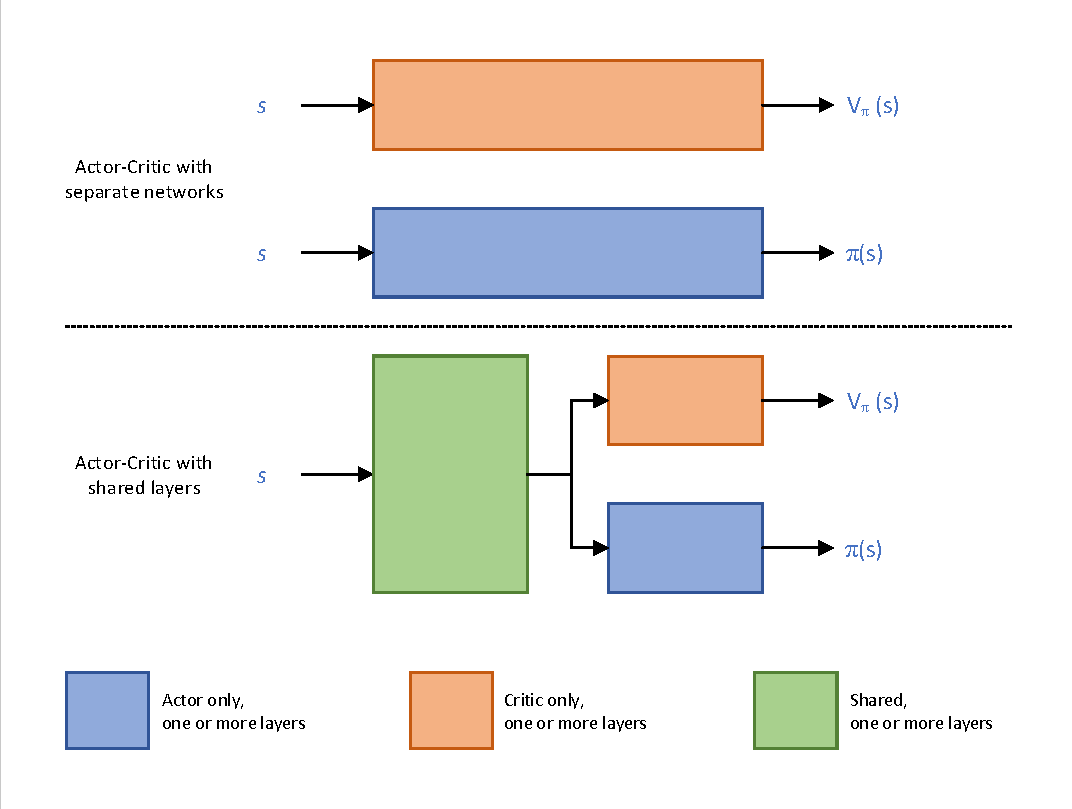
\includegraphics[clip, trim=10px 10px 10px 10px, width=0.85\columnwidth]{figures/rl/Actor_Critic_Architecture.pdf}
  \end{center}
  
  %\vspace*{-6pt}
  \caption[Actor-Critic Network Architectures]{Network architecture variants for actor-critic algorithms. The networks might be separate or with shared layers. (Adapted from \cite{foundations2019graesser})}
  \label{fig:actor_critic_architecture}
  %\vspace*{-12pt}
\end{figure}

We illustrated an example for the actor-critic network architecture in Figure \ref{fig:actor_critic_architecture}. While we could build the actor and the critic separately with two different networks, they will usually be constructed with a single network with separated network heads. The network then shares a certain amount of layers which learn basic feature representations. For example if we are dealing with images as input and are using a CNN to process them, the convolutional layers should be shared between the actor and the critic. This improves efficiency as we do not need to learn the feature representation twice. Since both the actor and the critic are propagating their error through the upper layers, they can be trained faster and unstable learning is reduced. After the shared layers, the actor and the critic have their own dedicated network output, which can consist out of a single layer or can be a complex network on its own. 

\begin{algorithm}[ht]
  \KwData{Actor learning rate $\alpha_A$, Critic Learning Rate $\alpha_C$ Entropy coefficient $\beta$}
  \KwResult{Optimized parameters for the actor $\theta_A$ and critic $\theta_C$}
  Initialize all the weights $\theta$ randomly \;
  \ForEach{episode}  {
   Sample trajectory $\tau = ((s_0, a_0, r_0), \dots, (s_T, a_T, r_T))$ with $\pi_\theta$ from the environment \;
    \For{$t=0, \dots, T$}  {
      $R_t(\tau) = \sum^T_{t'=t} \gamma^{t'-t}r_t$ \;
      Calculate $V_{\theta_C}(s_t)$ using the value network \;
      Calculate Entropy $H_t = - \sum_a \pi_{\theta_A}(a|s_t) \log \pi_{\theta_A}(a|s_t)$
    }
    \tcc{Calculate loss}
    $\mathcal{L}_{val}(\theta_C) = \frac{1}{T} \sum^T_{t=0}(V_{\theta_C}(s_t) - R_t(\tau))^2$ \tcp*{Value loss using MSE}

    $\mathcal{L}_{pol}(\theta_A) = \frac{1}{T} \sum^T_{t=0}\left(\left(V_{\theta_C}(s_t)-R_t(\tau)\right) \log \pi_{\theta_A}(a_t|s_t) - \beta H_t\right)$ \tcp*{Policy loss}

    \tcc{Update parameters with SGD optimizer}
    $\theta_C \leftarrow \theta_C - \alpha_C \nabla_{\theta_C} \mathcal{L}_{val}(\theta_C)$ \tcp*{Update Critic}
  
    $\theta_A \leftarrow \theta_A - \alpha_A \nabla_{\theta_A} \mathcal{L}_{pol}(\theta_A)$ \tcp*{Update Actor}

  }

  \caption[The Vanilla Actor-Critic Algorithm]{The vanilla actor-critic algorithm with entropy regularization.}\label{alg:ActorCritic}
 \end{algorithm}

The vanilla actor-critic method can be trained in a similar fashion as we did with REINFORCE and is shown in Algorithm \ref{alg:ActorCritic}. We changed a few things from REINFORCE, so lets quickly go through them:
\begin{itemize}
  \item We changed our notion for the application of the gradients. While we directly collected the gradients in Algorithm \ref{alg:REINFORCE}, we now calculate a loss. This makes it easier to add additional goals to the optimization (e.g. entropy). The loss is later converted into a gradient and applied by the SGD optimizer. Because we are now dealing with loss and the goal is to minimize the loss we have to change sign. By minimizing the loss we are performing gradient ascent on our objective function.
  \item We introduce integrated exploration and regularization with the addition of the entropy $H$ to the loss as we discussed in Section \ref{ssec:ImprovingPG}. The entropy is added to the loss for the actor and can be scaled with a new hyperparameter $\beta$.
  \item We are still using a for-loop over episodes, but it is possible to substitute this loop with a loop over an arbitrary number of individual steps (see Algorithm \ref{alg:PPO}).   
\end{itemize}

\paragraph{Estimating Advantage.}
The vanilla actor-critic algorithm is usually not used on its own. Instead a first extension is used: The \textit{Advantage Actor-Critic} (A2C) algorithm. When we talked about DQN Extensions in Section \ref{ssec:DQNExtensions} we briefly mentioned the advantage function $A(s, a)$. The advantage is a measure of how good an action is compared to all other actions. For DQN we compared the action only to other actions given that we know the optimal policy. This resulted in a maximal advantage of zero for the best action and a negative advantage for all other actions. This time we are instead looking at $A_\pi(s, a) = Q_\pi(s, a) - V_\pi(s)$. This is the advantage which measures the change in return if we take action $a$ and then always act according to our current policy. In other words, the advantage provides us with a relative measure of how good an action is compared to the average action our policy would choose. Before we look at how to estimate the advantage, let us first discuss why we should even care about advantage. Why do we need advantage when we have state-values?

Remember that we are currently training our policy by computing gradients based on the return we get by following the current policy in the environment. Our goal is to reinforce good actions and discourage bad actions. Since we compute our gradients from the return, we need the return to be negative for bad and positive for good actions to actually compute gradients which reflect reinforcement or discouragement of actions. Unfortunately this is not what usually happens: Many environments do not provide negative but only positive reward. So all actions are actually reinforced. To change this we need a relative measure which tells us how good an action is compared tp all other actions and this is exactly what the advantage function does. 

To compute the advantage we need two things: $V_\pi(s)$ and $Q_\pi(s, a)$. Currently our network only computes the value function, so should we further extend it to also compute the Q-Values? While this would be possible, it actually adds overhead into the network and Q-Values are harder to estimate than state-values, since Q-Value functions are more complex. Also learning Q-Values in continuous environments produces additional problems. So instead we want to estimate the Q-Values from the already estimated state-values. If we assume, that our estimate $V_\pi(s)$ is sufficiently accurate, we can estimate the Q-Value by:

\begin{align*}
Q_\pi(s_t, a_t) &= E_{\tau\sim\pi}\left[r_t + \gamma r_{t+1} + \gamma^2 r_{t+2} \dots + \gamma^n r_{t+n}\right] + \gamma^{n+1}V^*(s_{t+n+1}) \\
&\approx r_t + \gamma r_{t+1} + \gamma^2 r_{t+2} \dots + \gamma^n r_{t+n} + \gamma^{n+1}V_\pi(s_{t+n+1}) \\[15pt]
A_\pi(s_t, a_t) &= Q_\pi(s_t, a_t) - V_\pi(s_t) \\
&\approx r_t + \gamma r_{t+1} + \gamma^2 r_{t+2} \dots + \gamma^n r_{t+n} + \gamma^{n+1}V_\pi(s_{t+n+1}) - V_\pi(s_t)
\end{align*}

Using this $n$-step unrolling technique, we can estimate the Q-value with $n$ as a tradeoff parameter between variance and bias. Using more steps reduces bias, since $V_\pi(s)$ may be inaccurate, but at the same time it induces variance, since all rewards are sampled from a single trajectory. The idea is that variance increases the further we look into the future starting at step $t$ while the bias decreases. This means we are combining both to get the best result. Unfortunately deciding for an $n$ is not an easy choice and would require careful tuning. Therefore unrolling is done with a similar technique called \textit{Generalized Advantage Estimation} (GAE) which was proposed by Schulman et al. in 2015 \cite{schulman2015high}. Instead of using a fixed $n$ we instead compute the advantage using a weighted average over $n$-step advantages with $n = 1, 2, 3, \dots, k$. This technique further reduces the influence of variance and bias, while also making the choice of a hyperparameter easier. GAE can be written as:

\begin{align*}
  A_\pi(s_t, a_t) &= \sum^\infty_{l=0} (\gamma\lambda)^l \delta_{t+l} \\
  &\text{with } \delta_t = r_t + \gamma V_\pi(s_{t + 1}) - V_\pi(s_t) 
\end{align*}

While GAE still introduces a new hyperparameter in the form of $\lambda$ which controls how much we weight estimated advantages with further unrolling, this parameter does not introduce a hard boundary and therefore is much easier to tune. 

\begin{algorithm}[ht]
  \KwData{Actor learning rate $\alpha_A$, Critic Learning Rate $\alpha_C$ Entropy coefficient $\beta$}
  \KwResult{Optimized parameters for the actor $\theta_A$ and critic $\theta_C$}
  Initialize all the weights $\theta$ randomly \;
  \ForEach{episode}  {
   Sample trajectory $\tau = ((s_0, a_0, r_0), \dots, (s_T, a_T, r_T))$ with $\pi_\theta$ from the environment \;
    \For{$t=0, \dots, T$}  {
      Calculate $V_{\theta_C}(s_t)$ using the value network \;
      Calculate the advantage $A_\pi(s_t, a_t)$ using GAE. \;
      Calculate $V_{tar}(s_t)$ using the advantage. \;
      Calculate Entropy $H_t = - \sum_a \pi_{\theta_A}(a|s_t) \log \pi_{\theta_A}(a|s_t)$ \;
    }
    \tcc{Calculate loss}
    $\mathcal{L}_{val}(\theta_C) = \frac{1}{T} \sum^T_{t=0}(V_{\theta_C}(s_t) - V_{tar}(s_t))^2$ \tcp*{Value loss using MSE}

    $\mathcal{L}_{pol}(\theta_A) = \frac{1}{T} \sum^T_{t=0}\left(-A_\pi(s_t, a_t) \log \pi_{\theta_A}(a_t|s_t) - \beta H_t\right)$ \tcp*{Policy loss}

    \tcc{Update parameters with SGD optimizer}
    $\theta_C \leftarrow \theta_C - \alpha_C \nabla_{\theta_C} \mathcal{L}_{val}(\theta_C)$ \tcp*{Update Critic}
  
    $\theta_A \leftarrow \theta_A - \alpha_A \nabla_{\theta_A} \mathcal{L}_{pol}(\theta_A)$ \tcp*{Update Actor}

  }

  \caption[The Advantage Actor-Critic Algorithm]{The Advantage Actor-Critic (A2C) algorithm with entropy regularization.}\label{alg:A2C}
 \end{algorithm}

Algorithm \ref{alg:A2C} shows an updated version of the original actor-critic algorithm with GAE. Note that in praxis $V_{tar}$ is often calculated as $V_{tar} = A_{GAE}(s_t, a_t) + V_\pi(s_t)$ when using advantage estimation to avoid additional computation. 

\paragraph{Parallel environment interactions.}
We already developed techniques to solve most of the problems shown in Section \ref{ssec:ImprovingPG}, but there is still one remaining problem: Sample correlation. Since we cannot introduce a replay buffer - we are dealing with an on-policy algorithm - we have to generate a lot of training data to reduce sample correlation and variance before each update. Sampling all that data from a single environment running in a single process takes a lot of time and since episodes may be significantly dependent on the random initial state, we would need the agent to play through several whole episodes to gather good training data. In 2016 Mnih et al. showed, that it is possible to train an A2C agent in parallel on multiple environments with their \textit{Asynchronous Advantage Actor-Critic} (A3C) algorithm \cite{mnih2016asynchronous}.

When training the agent in parallel on multiple environments we want to create multiple copies of the same environment (and our agent) which gather trajectories independent of each other. Further, we want to initialize them with a different random seed to generate different trajectories due to randomness in environment transitions or agent action choices. The workers then continuously gather the training data from agent-environment interactions. This data will be used to calculate updates for a global network, which will then be pushed back to the workers periodically. This procedure can be done in two different ways: Synchronous and Asynchronous. Though A3C only uses asynchronous parallelization we will also briefly discuss synchronous parallelization as well.
\begin{itemize}
  \item \textbf{Synchronous Parallelization.} In synchronous parallelization all workers are working with the same copy of the network. Workers will gather a trajectories of a certain length and then wait for all other workers to finish. The trajectories are then combined and used to update the global network. After the global network has updated, each worker pulls the updated parameters to its own network copy and then continuous to collecting new trajectories. This type of parallelization is often used for A2C. The use of dedicated network copies can be avoided, if training is only done on a single machine.
  \item \textbf{Asynchronous Parallelization.} In asynchronous parallelization workers also collect trajectories, but they additionally compute the gradients and then directly push the gradients to the global network. The workers do not wait for each other and thus may work with a slightly outdated network copy. 
\end{itemize}
Both parallelization methods have their pros and cons. While synchronous parallelization works well on a single machine, the waiting mechanism may significantly slow down a distributed training processes. On the other hand for non-blocking asynchronous parallelization, the computation of gradients on slightly outdated network copies makes training less stable. Nevertheless, both methods work well and vastly reduce the impact of sample correlation and variance for on-policy PG methods. 


\subsection{Proximal Policy Optimization} \label{ssec:PPO}
The A2C algorithm addresses every problem we talked about in Section \ref{ssec:ImprovingPG}. Still if we look at the learning curve in in Figure \ref{fig:a2c_cartpole} which shows the training progress on the simple environment CartPole, we can see that learning tends to still be unstable and even suffers from \textit{performance collapse}. How is that possible? To understand the origin of this problem, we need to look back at our basic procedure of how we are improving our policy using policy gradients.

\begin{figure}[ht]
  
  \begin{center}
      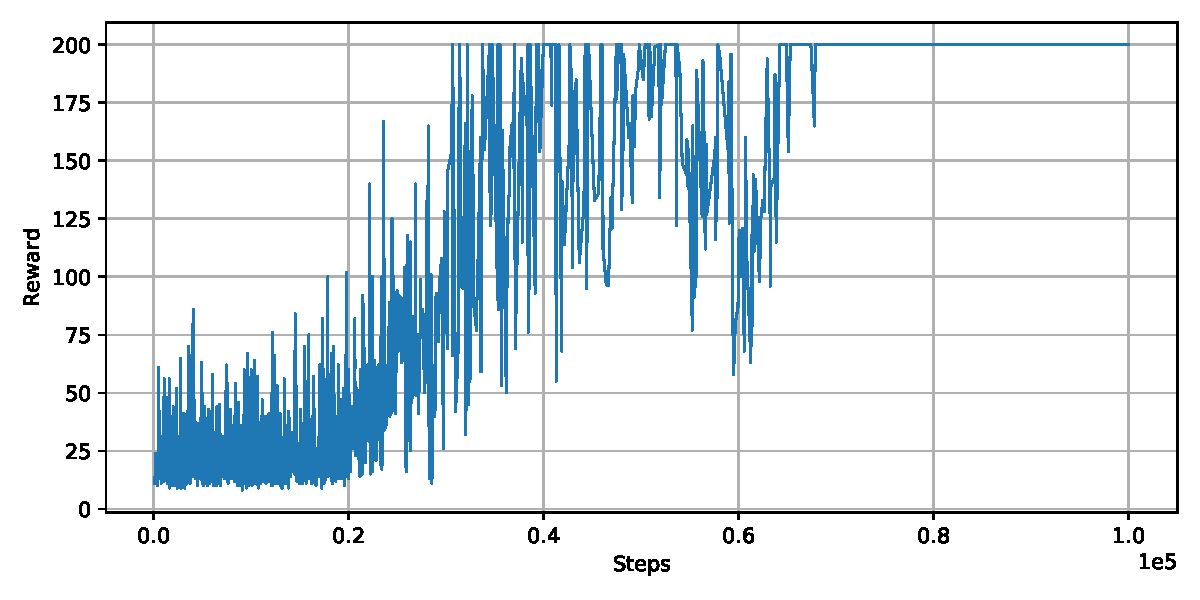
\includegraphics[clip, width=0.8\columnwidth]{figures/rl/a2c_cart_pole_plot.pdf}
  \end{center}
  
  %\vspace*{-6pt}
  \caption[Learning Curve for A2C on CartPole]{Reward per episode for an agent trained with the A2C algorithm on the CartPole environment over $100k$ training steps (roughly 600 episodes). Notice the brief performance collapse around 600k training steps.}
  \label{fig:a2c_cartpole}
  %\vspace*{-12pt}
\end{figure}

In PG algorithms, we use a policy $\pi_\theta$ which is parameterized by the weights of our neural network. This policy is used to generate a trajectory in our environment from which we compute the policy gradient $\nabla_\theta J(\pi_\theta)$. During optimization we therefore generate a sequence of policies $\pi_1, \pi_2, \dots, \pi_n$ from the the policy space $\Pi$ (the set of all policies). The problem is we are not actually directly searching for a policy in that space. Instead we are searching the policy in the parameter space $\Theta = \{\theta \in \mathbb{R}^m\}$ with $m$ being the number of parameters in our network. Unfortunately distances in policy space and in parameter space are not the same with respect to $\theta$. If we take two pairs of parameters $(\theta_1, \theta_2)$ and $(\theta_2, \theta_3)$ with the same distance in the parameter space, their mapped policies in policy space might not have the same distance:

\[d(\theta_1, \theta_2) = d(\theta_2, \theta_3) \cancel{\Leftrightarrow} d(\pi_{\theta_1}, \pi_{\theta_2}) = d(\pi_{\theta_2}, \pi_{\theta_3}) \]

The hypersurface on which we are performing our gradient ascent is not equal to the hypersurface we actually care about. This produces a semantic gap in our training process. Simply adjusting the learning rate $\alpha$ to a small value does not simply fix this problem. A small learning rate will only slow down learning and raise the probability of getting stuck in a local maximum. On the other hand we cannot accept occasional learning collapses, since learning collapses mean that we will immediately and dramatically reduce the quality of our training data. Recovering from a performance collapse can therefore take a long time. So how can we prevent them, while still learning in parameter space? The answer to this are \textit{trust regions}. The idea is to estimate the change in policy space. We then define a maximal distance "around" our old policy in policy space - called trust region - which is the maximum distance the new policy is allowed to deviate from the old policy. Moreover we want to guarantee, that the performance of the new policy is always better than the performance of the old policy.

In 2015 Schulman et al. were able to provide mathematical foundations with made the computation of trust regions and \textit{guaranteed monotonic improvement} of the policy possible. They also proposed an algorithm called \textit{Trust Region Policy Optimization} (TRPO) \cite{schulman2015trust}. Unfortunately even though their algorithm works, it is hard to implement and computationally very expensive, since it relies on second order derivates. To overcome these problems, they extended their work in 2017, proposing a simplified algorithm called \textit{Proximal Policy Optimization} (PPO) which even outperforms their pervious one in many environments \cite{schulman2017proximal}. PPO is computationally as expensive as vanilla actor-critic variants and thus PPO is one of the most used reinforcement learning algorithms today. In the remainder of this Section, we want to take a look at how PPO achieves its goal of monotonic policy improvement, while staying computationally inexpensive.

\paragraph{Monotonic Improvement.}
Instead of trying to directly maximize the expected return $J(\pi)$, we can instead maximize a different objective. To achieve monotonic improvement, we formulate a new objective based on the \textit{relative policy performance identity}. If we have some policy $\pi$ and update that policy to get $\pi'$, we define their relative policy performance identity as

\begin{equation} \label{eq:MonotonicImprovement}
  J(\pi') - J(\pi) = E_{\tau \sim \pi'}\left[\sum_{t\geq0} A_\pi(s_t, a_t)\right]
\end{equation}

which is their difference in expected return. With this objective our optimization problem becomes $\max_\pi' (J(\pi') - J(\pi))$ which ensures, that $J(\pi') - J(\pi) \geq 0$. The worst case is simply not changing the policy, such that $\pi'=\pi$.

The problem with Equation \ref{eq:MonotonicImprovement} is that it uses an expectation over a trajectory sampled from $\pi'$ - which we obviously do not have access to at that point. We therefore need a way to estimate trajectories from $\pi'$. If we assume that two successive policies $\pi$ and $\pi'$ are relatively close, we can also assume that the resulting state distributions we observe when interacting with the environment are also similar. Therefore we can use a method known as \textit{importance sampling} which estimates an unknown distribution from data sampled from a known distribution. This is done by computing weights which increase rewards which are more likely under $\pi'$ and decrease rewards which are less likely. These weights are calculated by the ratio of action probabilities between $\pi$ and $\pi'$: $\frac{\pi'(a_t, s_t)}{\pi(a_t, s_t)}$. We then can estimate the relative policy performance identity by

\begin{equation}
  J(\pi') - J(\pi) = E_{\tau \sim \pi}\left[\sum_{t\geq0} A_\pi(s_t, a_t) \frac{\pi'(a_t, s_t)}{\pi(a_t, s_t)}\right] = J^{CPI}_\pi(\pi')
\end{equation}

thus being only dependent on samples generated by the current policy. The new objective called the \textit{conservative policy iteration} (CPI) $J^{CPI}_\pi(\pi')$  is also called the \textit{surrogate objective}, since it indirectly optimizes the original objective. It can be proven that the gradient with respect to $\theta$ of the surrogate objective is equal to the gradient of the original objective. We omit the proof here, but it can be found in \cite{foundations2019graesser}. 

If the gradient of the original and the surrogate objective is the same, one could ask the question why we even need the new objective. Also we only approximate $J(\pi') - J(\pi)$, so how do we guarantee that $J(\pi') - J(\pi) \geq 0$? The reason behind our new objective is that it allows us to bound the error. Achim et al. \cite{achiam2017constrained} showed that using the Kullback-Leibler (KL) divergence between two successive policies, we can bound the error to

\[|(J(\pi') - J(\pi)) - J^{CPI}_\pi(\pi')| \leq C \cdot \sqrt{E_t\left[KL\left(\pi'(a_t, s_t)||\pi(a_t, s_t)\right)\right]}\]

From this, we can easily derive a form which allows us to determine if $J(\pi') - J(\pi) \geq 0$:

\begin{equation} \label{eq:MonotonicImprovement2}
  J(\pi') - J(\pi) \geq J^{CPI}_\pi(\pi') - C \cdot \sqrt{E_t\left[KL\left(\pi'(a_t, s_t)||\pi(a_t, s_t)\right)\right]}
\end{equation}

Looking at Equation \ref{eq:MonotonicImprovement2} we can see, that $J(\pi') - J(\pi) \geq 0$ only holds, if $J^{CPI}_\pi(\pi')$ is greater than the maximum error. If we only update our policy if this condition holds, we can guarantee policy improvement even if we only estimated  $J(\pi') - J(\pi)$. In a worst case scenario the best new policy will be the old policy, since if $J^{CPI}_\pi(\pi') = 0$ and $KL(\pi||\pi) = 0$ we can still accept the old policy as new policy. Using Equation \ref{eq:MonotonicImprovement2} we can finally formulate an updated version of the optimization problem:

\[\argmax_{\pi'}(J^{CPI}_\pi(\pi') - C \cdot \sqrt{E_t\left[KL\left(\pi'(a_t, s_t)||\pi(a_t, s_t)\right)\right])}\]

The remaining question now is how to implement this optimization problem in practice. Usually the error term is directly bounded to some constant $\delta$ which directly limits how large the KL divergence can be:

\[E_t[KL(\pi_\theta(a_t|s_t)||\pi_{\theta_{old}}(a_t|s_t))] \leq \delta\]

Of course $\delta$ is a hyperparameter that must be tuned for each individual RL problem. Since we are usually learning from a single step (or a small batch), our expectation is also written as an expectation over a single step. Since we are maximizing our objective in parameter space we are now writing our equation as dependent on these parameters $\theta$, with $\pi' = \pi_\theta$ and $\pi = \pi_{\theta_{old}}$. Therefore we arrive at the final surrogate objective:

\begin{align*}
  &\max_\theta E_t\left[\frac{\pi_\theta(a_t|s_t)}{\pi_{\theta_{old}}(a_t|s_t)}A_{t,\pi_{\theta_{old}}} \right] \\
  &\text{subject to } E_t[KL(\pi_\theta(a_t|s_t)||\pi_{\theta_{old}}(a_t|s_t))] \leq \delta
\end{align*}

With this surrogate objective we are now maximizing a linear approximation of $J(\pi') - J(\pi)$ with an imposed trust region, limiting the difference between the old and the new policy and thus avoiding performance collapse. Our new objective also now guarantees monotonic improvement.

\paragraph{The PPO Algorithm.}
The \textit{Proximal Policy Optimization} (PPO) algorithm was proposed by Schulman et al. in 2017 \cite{schulman2017proximal}. It uses the idea of trust regions with a minimum of additional computation. It also replaces the hyperparameter $\delta$ with a new hyperparameter which is easier to tune. In their original paper Schulman et al. proposed two different variants for the trust region constraint: An adaptive KL penalty - which uses a variable $\delta$ - and a clipped objective. In their tests, both variants proved to have good performance, but since the clipped objective is easier to tune, easier to implement and at least as good as the version with the KL penalty we will omit further details on adaptive KL penalty. 

To simplify our equations and add a little more clarity we will only write $A_t$ for $A_{t, \pi_{\theta_{old}}}$ in the following. We also define our probability ratio as $r_t(\theta) = \frac{\pi_\theta(a_t|s_t)}{\pi_{\theta_{old}}(a_t|s_t)}$. This way we can rewrite our surrogate objective as

  \[J^{CPI}(\theta) = E_t\left[\frac{\pi_\theta(a_t|s_t)}{\pi_{\theta_{old}}(a_t|s_t)}A_{t, \pi_{\theta_{old}}}\right] = E_t[r_t(\theta)A_t]\]

We will now take a look at the \textit{clipped surrogate objective}, which adds a clipping term to $J^{CPI}$:

\[J^{CLIP}(\theta) = E_t[\min(r_t(\theta)A_t, clip(r_t(\theta), 1-\epsilon, 1+\epsilon)A_t)]\]

The interesting thing is, that we can use this objective without adding a constraint for the KL divergence. The reason behind this can be explained by looking at the possible ways to maximize $J^{CPI}$. If we look at one step of training and some $A_t > 0$ one option to maximize $J^{CPI}$ would be to just perform a large policy update - thus maximizing $r_t(\theta)$. This is not what we want, because we already know that we are optimizing in parameter space and large policy updates are risky. In $J^{CLIP}$ we therefore clip the value of $r_t(\theta)$ to an $\epsilon$-neighborhood between $(1-\epsilon)A_t$ and $(1+\epsilon)A_t$. As long as $r_t(\theta)$ is in the interval $[1-\epsilon, 1+\epsilon]$, $J^{CLIP}$ is equal to $J^{CPI}$, but as soon as the new action probability diverges too much from the old policy the value is clipped. Hence, policy updates under the clipped objective function are always safe and we do not need an additional constraint.

\begin{algorithm}[h!]
  \KwData{Actor learning rate $\alpha_A$, Critic Learning Rate $\alpha_C$ Entropy coefficient $\beta \geq 0$, Clipping variable $\epsilon \geq 0$, Number of Epochs $K$, Number of Actors $N$, Time Horizon $T$}
  \KwResult{Optimized parameters for the actor $\theta_A$ and critic $\theta_C$}
  $M \leftarrow NT$ \;
  Initialize all the weights $\theta$ randomly \;
  Initialize the old actor network $\theta_{A_{old}}$ \;
  \For{$i=1, 2, \dots$}  {
    $\theta_{A_{old}} \leftarrow \theta_A$ \;
    \For{$actor = 1, 2, \dots, N$}{
      Sample trajectory $\tau = ((s_0, a_0, r_0), \dots, (s_T, a_T, r_T))$ from the environment with policy using $\theta_{A_{old}}$. \;
      Calculate $V_{\theta_C}(s_0), \dots V_{\theta_C}(s_T)$ using the value network \;
      Compute advantages $A_0, \dots, A_T$ using $\theta_{A_{old}}$ \;
      Calculate $V_{tar}(s_0), \dots V_{tar}(s_T)$ using the advantage and the value network $\theta_C$. \;
    }
    Construct a \textit{batch} with size $M$ from trajectories, advantages and target V-values. \;

    \For{$epoch=1, 2, \dots, K$}{
      \ForEach{minibatch $m$ in \textit{batch}}{
        \tcc{The following are computed over the whole batch}
        Calculate $r_m(\theta_A)$ \;
        Calculate $J^{CLIP}_m(\theta_A)$ using advantages $A_m$ and $r_m(\theta_A)$ \;
        Calculate entropies $H_m$ using actor network $\theta_A$ \;
        
        \tcc{Calculate loss}
        $\mathcal{L}_{val}(\theta_C) = \frac{1}{M} \sum^M_{t=0}(V_{\theta_C}(s_t) - V_{tar}(s_t))^2$ \tcp*{Value loss using MSE}
    
        $\mathcal{L}_{pol}(\theta_A) = \frac{1}{M} \sum^M_{t=0}\left(J^{CLIP}_t(\theta_A) - \beta H_t\right)$ \tcp*{Policy loss}

        \tcc{Update parameters with SGD optimizer}
        $\theta_C \leftarrow \theta_C - \alpha_C \nabla_{\theta_C} \mathcal{L}_{val}(\theta_C)$ \tcp*{Update Critic}
      
        $\theta_A \leftarrow \theta_A - \alpha_A \nabla_{\theta_A} \mathcal{L}_{pol}(\theta_A)$ \tcp*{Update Actor}

      }

    }

  }

  \caption[The PPO Algorithm with Clipped Surrogate Objective]{The PPO algorithm with clipped surrogate objective as an extension to synchronous parallelized A2C. (Adapted from \cite{foundations2019graesser}.)}\label{alg:PPO}
 \end{algorithm}


Removing the KL divergence constraint makes the clipped objective function computationally inexpensive. The only computations that are done are the probability ratio $r_t(\theta)$ and the advantage $A_t$. Both of them are the minimal computational cost we have to invest for any policy update. Algorithm \ref{alg:PPO} shows PPO with a clipped objective function as an extension of the actor-critic algorithm from Section \ref{ssec:A2C}. We also use synchronous parallelization.

 The algorithm shown has some major differences with the original A2C algorithm from Algorithm \ref{alg:A2C} so lets go over them:
\begin{itemize}
  \item We got a few new hyperparameters. The number of actors defines the number of parallel agents. We will talk about the number of epochs and the time horizon later on.
  \item \textit{Line 4}: Our Main loop changed from episodes to an infinite loop. Usually this outer loop will train for a fixed number of steps.
  \item \textit{Lines 6-11}: Each actor trains for a set amount of steps in its own copy of the environment. We call this amount of steps the \textit{Time Horizon} $T$. Since we are using the synchronous variant of A2C, each actor uses the same network weights. After sampling the trajectory we are computing state values and estimating advantages via GAE for each step. We are also computing the V-target values.
  \item \textit{Lines 12-14}: After we have generated the trajectories and computed state-values and advantages, we create a batch for the network updates. Since the objective function only needs samples from the old policy $\pi_{\theta_{old}}$, we can use data from the trajectory multiple times. This increases sample efficiency. We create random samples from of our batch of training data with size $T$. These smaller batches are called \textit{minibatches} and we compute a parameter update for each of them. We will repeat this for $K$ epochs.
  \item \textit{Lines 15-21}: We calculate the probability ratio $r_m(\theta_A)$ our objective $J^{CLIP}_m(\theta_A)$ and the entropy $H_m$ based on the current minibatch. We then calculate the loss for the actor and the critic and apply the resulting gradients with the SGD optimizer of choice. 
\end{itemize}

\subsection{Alternative Actor-Critic Algorithms} \label{ssec:AlternativeCombinedMethods}
We already presented one of the most well-known members of the actor-critic family - the PPO algorithm - in Section \ref{ssec:PPO}. In this section we want to give a short introduction into two additional members of the actor-critic family: ACER which aims at improving sample-efficiency by making it possible to learn from past experiences and ACKTR, which proposes an alternative trust region algorithm. 

\paragraph{ACER.}
\textit{Actor-Critic with Experience Replay} (ACER) was developed in 2016 by Wang et al. \cite{wang2016sample}. The goal of ACER was to create an actor-critic successor which could handle off-policy training and thus being more sample efficient. ACER also implements trust-region policy optimization.

At its base, ACER changes the actor-critic architecture to learn Q-Values instead of state-values. They do this, by using the Retrace algorithm by Munos et al. \cite{munos2016safe} which estimates target Q-Values with minimal bias and variance and has been proven to converge:

\begin{align*}
  &Q^{ret}(s_t, a_t) = r_t + \gamma \bar{r}_{t+1}(\theta) \left[Q^{ret}(s_{t+1}, a_{t+1}) - Q_\pi(s_{t+1}, a_{t+1})\right] + \gamma V_\pi(s_{t+1}) \\
  &\text{with } \bar{r}_t(\theta) = \min(c, r_t(\theta))
\end{align*}

After sampling a trajectory we can compute the values for $Q^{ret}$ from the last timestep backwards, since $Q^{ret}(s_T, a_T) = 0$. We can then use $Q^{ret}$ as target value and compute the mean square error loss for backpropagation. 

For the training of the actor, ACER also uses the target Q-Values. Similar to PPO, sample returns will be weighted by the probability ratio between the old and the new policy $r_t(\theta)$. Learning from old trajectories requires to save the probability distribution over actions from the current policy in the replay buffer. The problem for off-policy training is that the importance weights may become very large over time (since the current and some old policy may produce vastly different probability distributions for some state) causing training to become unstable. To prevent this, the importance weights are clipped to a fixed value $c$. To ensure an unbiased estimation they also add a correction term which is called the \textit{truncation with bias correction trick} 

\begin{align*}
  \mathcal{L}^{acer}_{pol}(\theta_A) = &\bar{r}_t(\theta) \log \pi_A(a_t|s_t)[Q^{ret}(s_t, a_t) - V_{\theta_C}(s_t)] \\ 
  &+ E_{a\sim\pi} \left(\left[\frac{r_t(\theta, a) - c}{r_t(\theta, a)}\right]_{+} \log \pi_{\theta_A}(a|s_t)[Q_{\theta_C}(s_t, a) - V_{\theta_C}(s_t)] \right)
\end{align*}

\begin{align*}
  &\text{with } r_t(\theta, a) = \frac{\pi_\theta(a|s_t)}{\pi_{\theta_{old}}(a|s_t)} \\
  &\text{and } [x]_+ = 
  \begin{cases} 
    x, & \text{if}\ x > 0 \\
    0, & \text{otherwise}
  \end{cases}  
\end{align*}
 

The above expression also uses a baseline $V_{\theta_C}(s_t)$ which is subtracted to reduce variance. The first term is the standard loss, weighted by the clipped importance weights and the second term is the correction term.

We already saw that actor-critic variants may have problems when updating the policy, since updates take place in the parameter space. Similar to PPO, ACER uses a trust region when performing updates. However ACER uses a different method: Instead of constraining the policy to not deviate too much from its predecessor, ACER maintains an \textit{average policy network}. This network represents a running average of past policy networks. When updating, ACER computes the KL divergence between the new and the average policy network and thus bounds the policy from deviating too far.

\paragraph{ACKTR.} \textit{Actor Critic using Kronecker-Factored Trust Region} (ACKTR) has been developed in 2017 by Wu et al. \cite{wu2017scalable}. ACKTR combines an improved optimization method called \textit{natural gradient descent} with yet another idea of how to compute trust regions for actor-critic updates. ACKTR has proven to have higher sample efficiency and learn better results in less time than A2C or TRPO. 

Today most RL algorithms use stochastic gradient descent to calculate gradients for the network. SGD optimizers use first order derivates on the loss function, meaning they compute the slope of the loss function at a given point. First order derivates are fast and easy to compute and combined with extensions like momentum provide reasonably fast results. However by only looking at the first derivate, SGD is very sensitive to the learning rate. By calculating gradient updates based on the descent at the current point only, we do not take the change of descent into account. This means, that the direction of the gradients is not optimal and does not point directly into the direction of the optimum. Also we still have to face the problem we explored earlier: Changes to the weights are computed in parameter space assuming an equal change to the objective (in policy space). We saw, that it is possible to limit the change in policy space by setting an upper bound for the KL divergence - ensuring our new policy would be "close enough" to the old policy. But what if we were able to optimize our policy in policy space and compute the gradients in parameter space from there? This would not only solve the problem of diverging from the optimum, but also speed up learning, as our gradient descent would point directly to the optimum of the cost function.

In 1998, Shun-Ichi Amari presented his approach of using a \textit{natural gradient} instead of standard SGD \cite{amari1998natural}. The idea is that we build a connection between each parameter from our model (from parameter space) to the policy space which tells us how great of an impact the change of each parameter will have in policy space. This way we can compute the natural gradient as the largest change in objective per unit change in our model parameters. By performing these weighted gradient descent steps in parameter space the resulting changes in policy space will have equal distance.

If we look at gradient descent and some loss $\mathcal{L}(\theta)$, the steepest descent direction can be defined as the vector $d$ which minimizes $\mathcal{L}(\theta + d)$ under the constrained that the squared length of $|d|^2 \leq \epsilon$. This length of $d$ is $\sum_i (d_i)^2$ in an euclidean space and $\sum_{i, j} g_{i, j}d_i d_j$ in any arbitrary coordinate system. The values $g_{i, j}$ are given by a positive semi-definite matrix $G$. The second formula for the distance is equal to the first one if $G$ is the identity matrix $I$ (which is true for any euclidean space). Amari showed, that we can define the direction of the steepest gradient descent in any space as 

\[\tilde{\nabla}\mathcal{L}(\theta) = G^{-1}\nabla\mathcal{L}(\theta) \]

The matrix $G$ can be computed by using the \textit{Fisher Information Matrix} (FIM) as a replacement. The FIM defines how much information an observable random variable $X$ carries about the unknown parameters $\theta$ of a probability distribution $p$ on which $X$ depends. The FIM is given by 

\begin{align*}
  F &= E \left[\nabla_\theta \log p_\theta(y|x) \nabla_\theta \log p_\theta(y|x)^T\right] \\
  &\approx \frac{1}{N} \sum^N_{i=1} \nabla_\theta \log p_\theta(y|x_i) \nabla_\theta \log p_\theta(y|x_i)^T
\end{align*}

with an expectation over the data distribution of the training data. The probability distribution is our neural network (e.g. the actor policy $\pi_{\theta_A}$). The interesting property of the FIM is that it is equal to the Hessian (the second order derivate) of the KL-divergence. Therefore the FIM defines the local curvature in policy space. The natural gradient is therefore defined as:

\[\tilde{\nabla}_\theta\mathcal{L}(\theta) = F^{-1}\nabla_\theta\mathcal{L}(\theta)\]

The computation for natural gradient descent follows Algorithm \ref{alg:NaturalGradient} and is very similar to SGD with the exception of the computation of the FIM. 

\begin{algorithm}[h!]
  \KwData{Learning rate $\alpha$}
  \KwResult{Optimal parameters $\theta$ minimizing the loss function $\mathcal{L}(\theta)$}
  
  \While{Not Converged} {
    Compute the loss $\mathcal{L}(\theta)$ like before. \;
    Compute the gradient for the loss $\nabla_\theta \mathcal{L}(\theta)$ \;
    Compute the FIM from the trajectory. \;
    Compute the natural gradient $\tilde{\nabla}_\theta\mathcal{L}(\theta) \leftarrow F^{-1}\nabla_\theta\mathcal{L}(\theta)$ \;
    $\theta \leftarrow \theta - \alpha \tilde{\nabla}_\theta\mathcal{L}(\theta)$ \;
  }
  
  \caption[The Natural Gradient Descent Algorithm]{The Natural Gradient Descent Algorithm.}\label{alg:NaturalGradient}
 \end{algorithm}


In 2002 Sham Kakade was able to show that the natural gradient can be applied to policy gradient methods and converges faster than optimization with SGD in an RL setting \cite{kakade2002natural}. Unfortunately despite this proof of concept, the computation of the FIM is computationally very expensive. Even worse, for the size of nowadays neural networks with millions of parameters, the computation of the FIM would exceed main memory capacity. The only way we are able to use the FIM is to find a reasonably good approximation. 

In 2015 James Martens and Roger Grosse presented their novel method called \textit{Kronecker-Factored Approximate Curvature} (KFAC) \cite{martens2015optimizing} which is specifically designed to efficiently approximate FIM matrices for neural networks. The idea is to calculate approximations for the FIM layer-wise by assuming, that second-order statistics of the activations in layer $l$ and the backpropagated derivates are uncorrelated. While this assumption is not exact, in reality it still yields good results. KFAC can be used to train both the actor and the critic if we define the output of the critic as a Gaussian distribution - for which we can then can calculate the Fisher matrix. 
%Let $p(y|x)$ denote the output distribution of a neural network and $L = \log p(y|x)$ denote the log-likelihood. In the $l$th layer we have our weight matrix $W \in \mathbb{R}^{C_{out}\times C_{in}}$ where $C_{in}$ is the number of input neurons and $C_{out}$ is the number of neurons in the current layer. The current layer receives a vector $a \in \mathbb{R}^{C_{in}}$ from the $(l-1)$th layer and computes its output vector as a weighted sum $z = Wa$. Note that we did not apply the activation function yet. The weight gradient for our layer is then given by $\nabla_W L = (\nabla_sL)a^T$. We further define an operation $vec\{\}$ which vectorizes a matrix by stacking the columns on top of each other and denote the Kronecker product as $A \otimes B$ - which multiplies each element in matrix $A$ with matrix B such that $A \otimes B = (a_{i, j} B)$. We then can write the Fisher matrix for layer $l$ as 

%\begin{align*}
%  F_l &= E[vec\{\nabla_W L\}vec\{\nabla_W L\}^T] = E[aa^T \otimes \nabla_sL(\nabla_s L)^T \\
%  &\approx E[aa^T] \otimes E[\nabla_sL(\nabla_s L)^T]

%\end{align*}

Since we are only working on a approximation of the Fisher matrix and it was observed, that in the context of deep RL unbounded updates can still lead to large policy updates, ACKTR also uses a trust region method. Ba et al. showed, that since the Fisher matrix has a direct connection to the KL-divergence, it can be used as a replacement when formulating the trust region \cite{ba2016distributed}. This can be done by setting the effective step size $\eta$ for an update of the parameters to 
\[\eta = \min\left(\eta_{max}, \sqrt{\frac{2\delta}{\mathbf{v}^T\hat{F}\mathbf{v}}}\right)\]

where $\delta$ is the trust region radius, $\mathbf{v} = \Delta\theta$ is a vector representing the parameter change and $\hat{F}$ is the Fisher matrix approximation.
ACKTR has shown exceptional good performance in comparison with A2C and TRPO in both maximum performance and wall-clock time.


\subsection{Learning with Curiosity} \label{ssec:Curiosity}
So far all our agents tried to maximize one thing: The total reward they get from the environment. This behavior produces multiple problems: 

\begin{itemize}
  \item The agents behavior is directly dependent on the reward function, so correctly shaping the reward is crucially important for every new environment.
  \item If rewards are only given in a very sparse setting, agents may fail at exploring the environment to the point where they actually get rewarded. This also happens because the agent only learns from loss and the loss is only dependent on the reward. If our agent is not able to get any reward, it will be unable to learn anything.
  \item Even if the agent is able to learn, it may fail at deeply exploring the environment further, because every change in policy may result in less reward for the moment.
\end{itemize}

If we look at these problems, they are all related to a problem of exploring the environment. In the past, we explored the environment by random chance, but that does not seem to be sufficient. As a human, how do we get motivated to do something? Do we only learn or explore if we get rewarded for it by someone? The answer is no. We get reward, but it is not given to us, it is intrinsic to ourselves: We are curious about our surroundings and by satisfying that curiosity we generate "reward". Curiosity drives us to learn things that do not serve any need at the moment, but might become handy in the future. This idea motivates us to extend the basic reward function for our agent to include a term for curiosity.

Modeling curiosity for RL agents has been mainly explored in two different approaches: Encouraging the agent to explore novel states or encouraging the agent to perform actions which outcome cannot be predicted well. Measuring novelty has been shown to be difficult, since it requires to model the unknown statistical distribution of environmental states. In 2017 Pathak et al. proposed an \textit{Intrinsic Curiosity Module} (ICM) which generates intrinsic reward $r^i_t$ additional to the extrinsic reward $r^e_t$ from the environment \cite{pathak2017curiosity}. They showed, that it is possible to train agents using purely intrinsic reward and that agents trained with both intrinsic and extrinsic reward, outperform agents trained purely with extrinsic reward.

Let us take a look at how the ICM works. The idea of the ICM is to use prediction error as an indicator for curiosity reward. Intuitively this makes sense, since prediction error can be seen as the agent being surprised by a state. But we have to be slightly more precise when it comes to this error. Let us look at an example where the agent gets an observation from a camera. Under low light conditions the image will get more and more noisy, making situations with low light more interesting. Similar things are happening with various other things, like a TV outputting static noise, or leafs moving in the wind. In all these situations the observation (especially observations which are images) will change unpredictably and thus be surprising to the agent. We are therefore interested in a feature representation, which is only dependent on things the agent has influence over or which directly influence our agent in the environment. Everything else is just noise and should be ignored. 

To calculate the reward we will use an embedding network which transforms the observation of the current state into a representation $\phi(s)$. We will then use a \textit{forward dynamics network} which should predict the representation of the next state $\hat{\phi}(s_{t+1})$ from the current state and action the agent took in state $s_t$. This network can be expressed as $p(\phi(s_{t+1})|s_t, a_t)$. For a given transition tuple $(s_t, a_t, s_{t+1})$ the intrinsic reward is then given by the negative log likelihood $-\log p(\phi(s_{t+1})|s_t, a_t)$ and usually calculated using the mean square error of the forward dynamics network:

\[r^i_t = \frac{\eta}{2}||\hat{\phi}(s_{t+1}) - \phi(s_{t+1})||^2\]

with a scaling factor $\eta > 0$. The prediction error for a state will naturally be higher if the state or very similar states have not been often explored in the past, thus encouraging the agent to do so in the future.

Burda et al. investigated the performance of this intrinsic reward in combination with several feature spaces for forward dynamics \cite{burda2018large}. Two different approaches were found which both yield good results: 

\begin{enumerate}
  \item \textbf{Random Features (RF).} Random features are generated by a convolutional neural network. All parameters of that network will be fixed after the inital random initialization. This procedure results in stable features, but the features itself are not guaranteed to neither filter out any unnecessary information nor contain all necessary ones. Surprisingly random features still yield good results. Random features are easy to implement and do not require extra training time.
  \item \textbf{Inverse Dynamics Features (IDF).} Inverse dynamics features were initally proposed for the ICM and are generated by extending the embedding network with a second head. Given two states $s_t, s_{t+1}$ the network should predict the action $a_t$ the agent choses in state $s_t$. The networks first layers are used as a common neural network $\phi$ to embedd the observations. The idea is, that by training this network to also predict the action, the feature representation will be trained to ignore all aspects of the observation which are not under the agents immediate control. However this representation will not show aspects of the environment which will influence the agent but are not under its control.
\end{enumerate}

While both approaches have shown to work well with the ICM, they both failed at reliably eliminating the influence of stochastic transitions in the environment. Even with IDF features, if the agent has the possibility to influence the appearance of stochastic features (like randomly changing static noise on a TV) it would tend to only explore these stochastic states after some time. Also when using IDF we are dealing with stochasticity induced by sampling an action from our policy which cannot be predicted by our deterministic predictor network. Burda et al. therefore proposed a new approach which they called \textit{Random Network Distillation} (RND) in another paper \cite{burda2018exploration}.

RND is not an embedding for the observation and instead replaces the whole ICM. The intrinsic reward in RND is generated by a random prediction problem. This problem is build by two neural networks: The first network is called the \textit{target} network which is randomly initialized and fixed - similar to the random feature network from before. This target network takes the observation and transforms it into a random feature representation $f : \mathcal{O} \rightarrow \mathbb{R}^k$. We then construct a second network with the same architecture called the \textit{predictor} network which also takes the observation as input $\hat{f} : \mathcal{O} \rightarrow \mathbb{R}^k$. The predictor network is trained to minimize the mean square error between its own output and the target network $||\hat{f}(s) - f(x)||^2$. The idea is, that the prediction error will be larger for observations which are dissimilar to observation seen in the past. It could be shown, that gradient descent is unable to mimic the target network perfectly for any input and therefore the error can always be used to generate the intrinsic reward signal. 

The authors showed, that for actor-critic variants it can be beneficial to also modify the architecture to predict two state-values instead of one. The first value head predicts the state value for expected environment return (like before) and the second one predicts the value for the expected intrinsic reward. They showed that this method can improve learning further, if rewards are not clipped at the end of an episode (restart is just the next state). 

Curiosity - especially with RND - has shown to vastly improve the performance of PPO especially for environments with sparse reward. It also has been proven to be beneficial for environments with dense reward - leading to agents which learn both faster and reach a higher final reward. Curiosity can be combined with any RL algorithm, but only has been extensively studied in combination with PPO so far.

\chapter{Implementation} \label{chp:Implementation}
In this chapter we will take a look at different parts of the implementation. We will begin by discussing some general implementation notes in Chapter \ref{sec:ImplementationNotes} and the continue to present our experimentation environment called \textit{baselines lab} in Section \ref{sec:BaselinesLab}. We then talk about the particle simulation environment, including different scenarios from the original implementation of Huang et al. in Section \ref{sec:MazeEnvironment}.

\section{General Implementation Notes} \label{sec:ImplementationNotes}
Before talking about the actual implementation we want to talk a little bit about our general design choices. As a programming language we chose to use Python 3 \cite{van2011python, pythonWebsite}. Python is an interpreted high-level programming language with itself is written in C. Even though it is interpreted and thus may be slower than languages like C or C++, the easy integration of high-performance libraries which also scale into distributed systems make applications developed in python very fast. In the past years almost every ML library is developed for python making Python an ideal choice for data-science and machine learning projects.

The popularity of machine learning has lead to the developed of a number of libraries which support the creation and training of artificial neural networks. Modern libraries also especially leverage the computing power of the GPU to accelerate the computation of large matrix operations. Many of the libraries support more or less the same functionality, but may have a very different style of how certain things can be achieved. Currently the two most popular libraries for machine learning are PyTorch \cite{paszke2019pytorch} and Tensorflow \cite{abadi2016tensorflow}, we decided to use the latter. This decision was made in conjunction with our second big backend library which extends Tensorflow for reinforcement learning: Stable-Baselines \cite{stable-baselines}. Stable baselines offers high-quality implementations of many RL algorithms which are partially forked from the OpenAI Baselines project \cite{baselines}. While Google offers their own reinforcement library under the name TF-Agents \cite{TFAgents} we found that it currently is in a too early development state and thus not stable enough for the course of this thesis.

Since Python offers the easy integration of additional libraries we also make use of a number of additional libraries, most notably:
\begin{itemize}
    \item OpenAI Gym \cite{openAIgym} for a standardized environment creation as well as the integration of the Atari environments for testing purposes.
    \item OpenCV \cite{opencv_library} for image preprocessing.
    \item Numpy \cite{oliphant2006guide} for fast matrix computations.
    \item Optuna \cite{akiba2019optuna} for automated hyperparameter search.
\end{itemize}

\section{Baselines Lab} \label{sec:BaselinesLab}
To test out various combinations of reinforcement learning algorithms, their settings with different environments and environment settings we need a flexible and easy configurable program which also gives us the possibility to monitor the performance and create evaluations of trained models. While there already exist some projects which offer some of these features we did not find a project which was fully suited for our needs. The stable-baselines co-project baselines zoo \cite{rl-zoo} had to few options for the configuration of algorithms and while other libraries like slm-lab \cite{kenggraesser2017slmlab} did fit our need for configurability, they did not offer enough reinforcement learning algorithms. Therefore we decided to build our own lab environment on top of stable-baselines which we call \textit{Baselines Lab}.

\subsection{Basic Functions} \label{sec:blFunctions}
train, enjoy and search mode
session/trial -> Automated plots
automated saving/loading, logging -> tensorboard
Easy lab configuration via config files

\subsection{Random Network Distillation Module} \label{sec:blRND}
Unique RND implementation -> Staged as extension for SB3

\subsection{Automated Hyperparametersearch} \label{sec:blSearch}
Optuna and its basic functions, how to configure hyperparametersearch.

\subsection{Additional Functions} \label{sec:blAdvanced}
Automated video creation (enjoy, obs).
Learning rate schedules.
Email notification


\section{The Particle Maze Environment} \label{sec:MazeEnvironment}

\subsection{Basic Implementation} \label{sec:MazeImplementation}
Reimplementation of Huangs environment. Observations, etc

\subsection{Reward Shaping} \label{sec:MazeReward}
Rewards

\subsection{Extended Models} \label{sec:ExtendedMaze}
fuzzy, physical 

\subsection{Random Instance Generation} \label{sec:RandomInstanceGeneration}
random map generation

\section{Integration of Algorithmic Approaches} \label{sec:AlgorithmIntegration}
integration




\chapter{Evaluation} \label{chp:Evaluation}
In this chapter we want to present and discuss our evaluation results. Using Baselines Lab, we perform tests in a variety of different scenarios. After explaining our general test procedure in Section \ref{sec:TestProcedure}, we will begin, by evaluating the basic components for solving maze environments. In Section \ref{sec:EvalReward} we will take a look at reward generation and continue with a deeper look into observation generation and preprocessing in Section \ref{sec:EvalObs}. Section \ref{sec:EvalRLAlgorithms} will shine some light on the question which learning algorithm performs best when dealing with our particle navigation task and we will wrap up the evaluation of the basic parameters in Section \ref{sec:EvalParameters} where we take a look at the influence of various RL hyperparameters.

The initial tests will allow us to generate a baseline for the performance of our model, which then will be used throughout the rest of the evaluation to compare the influence of other factors. We begin, by testing how much inaccuracy in both actions and observations will influence the agent in Section \ref{sec:EvalError} and continue with the extension of the particle model with physical particles in Section \ref{sec:EvalPhysical}. We will then take a look at randomized instances in Section \ref{sec:EvalRandomness} and finish with a comparison with algorithmic approaches in Section \ref{sec:EvalAlgorithms}.


\section{Test Procedure} \label{sec:TestProcedure}
In this section we want to talk about different aspects of our test procedure.

\paragraph{Environment.}
All experiments were done on a Linux workstation running Ubuntu 18.04 LTS. The workstation has an Intel 6700K CPU, a single Nvidia GeForce GTX 1080 Ti GPU and 64GB of main memory. We installed Python 3.7.3 using the Anaconda \cite{anaconda} software distribution. We also used Tensorflow 1.14 in conjunction with the CUDA Toolkit version 10.1.243 and CUDNN version 7.6.5. Baselines Lab was developed on top of Stable-Baselines 2.10 and NumPy 1.17. For a complete list of installed packages see Appendix \ref{apx:BaselinesLab}.

\paragraph{Procedure.}
Our experiments involved several sources of randomness. To ensure consistent executions, we fixed the random seed for all involved components to the same value for all experiments. Unfortunately Tensorflow 1.14 does not guarantee consistent results during GPU computations. We therefore repeated experiments three times and averaged the results for comparison. The learning curves provided in this chapter are also smoothed by an exponential weighted moving average, using a factor of $0.6$.

To determine the performance of a configuration, we look at the end result during training for the average and best trial. We also determine the step in which the average episode length becomes smaller by five percent in comparison to the environments' time limit. We call this moment the \textit{drop}, since performance usually suddenly increases when the agent is able to reach the goal for the first time. The drop can be used as an indicator for how fast the agent is able to find a first usable result, while the end-of-training episode length is an indicator for how good the best solution is the agent is able to find. 

\paragraph{Initial Hyperparameters.}
For our initial experiments we wanted to use general purpose hyperparameters for the PPO algorithm. We therefore used parameters similar to the parameters used in the RND paper \cite{burda2018exploration} (see Table \ref{tab:PPOHyperparemeters}) which showed to produce good results across all Atari environments. 


\begin{table} [ht]
    \begin{center}
        \begin{tabular}{|c|c|}
            \hline
            Hyperparameter & Value \\
            \hline
            Rollout Length & 256 \\
            Number of minibatches & 8 \\
            Number of optimization epochs & 16 \\
            Number of parallel environments & 64 \\
            Learning rate & 0.0001 \\
            Optimization algorithm & Adam \cite{kingma2014adam} \\
            $\lambda$ & 0.95 \\
            Entropy coefficient & 0.001 \\
            $\gamma$ & 0.99 \\
            Clip range & [0.9, 1.1] \\
            \hline
        \end{tabular}
    \end{center}
    \caption[Default Hyperparameters]{Default hyperparameters for PPO for the initial experiments.} \label{tab:PPOHyperparemeters}
\end{table}

We also used a common preprocessing pipeline for the observations which was also used in previous experiments \cite{huang2019}:

\begin{table} [h]
    \begin{center}
        \begin{tabular}{|c|c|}
            \hline
            Hyperparameter & Value \\
            \hline
            Observation downsampling & (84, 84) \\
            Max steps per episode & 2000 \\
            Max and skip Frames & 4 \\
            Frame stacking & 4 \\
            \hline
        \end{tabular}
    \end{center}
    \caption[Default Observation Preprocessing]{Default observation preprocessing for all environments.} \label{tab:RNDPreprocessing}
\end{table}

If not stated otherwise, we also normalized the observations by $x \mapsto x/255$. Observations for the RND curiosity module are normalized by $x \mapsto CLIP((x-\mu)/\sigma, [-5, 5])$ instead and no frame stacking is applied.


\paragraph{Instances.}
To allow easy comparison, we used the same instances as in previous work for our experiments. We included a description of these instances in Table \ref{tab:TestInstances}. Previous work showed, that these instances provide a good scale of difficulty between easy (\texttt{Corridor}) and hard (\texttt{Brain}). Instances with less paths to the goal position seem to be harder to solve, since they require more precise manoeuvering instead of just pulling all particles into a general direction. To increase the difficulty of our medium instance, we replaced it with an instance generated by our RRT instance generator. This instance can also be seen in Table \ref{tab:TestInstances} and is called \texttt{Vessel}. The Vessel maze has similar dimensions in comparison with Corridor, but has far more fine grained structures where particles may get stuck. There is also only a single path to the goal position. Additionally the Vessel maze only has a small percentage of blocked pixels, allowing for a lot more possible states than Corridor. 

\begin{table} [h!]
    \begin{center}
        \begin{tabular}{cccccc}
            \toprule
            Instance & Name & Dimension & Size (\% of Area) & $d_{avg}$ & $d_{max}$ \\
            \midrule
            
            \parbox[c]{3.5cm}{
\includegraphics[clip, width=3.5cm]{figures/evaluation/procedure/corridor_upscaled.png}} & Corridor & $(100 \times 100)$ & $2869 \ (= 28.69\%)$ & 73.65 & 117 \\
            \addlinespace[0.05cm]
            \midrule
            
            \parbox[c]{3.5cm}{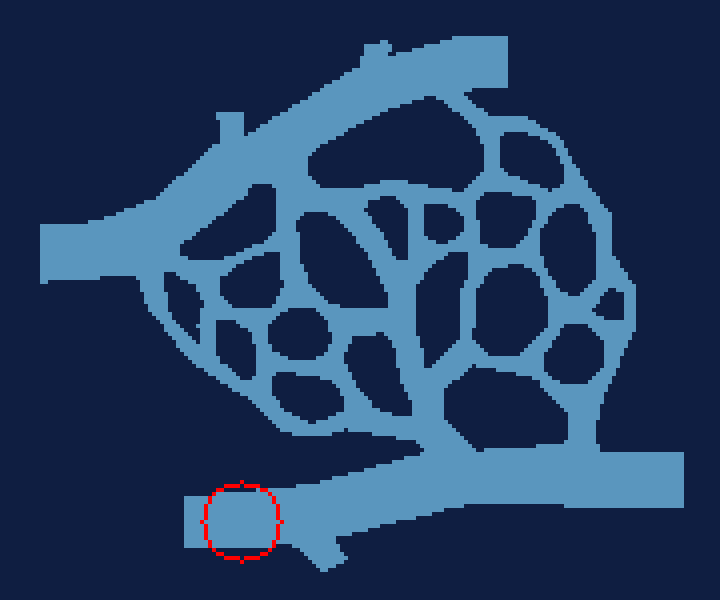
\includegraphics[clip, width=3.5cm]{figures/evaluation/procedure/capillary_upscaled.png}} & Capillary & $(180 \times 150)$ & $7169 \ (\approx 26.55\%)$ & 91.22 & 149 \\
            \addlinespace[0.05cm]
            \midrule
            
            \parbox[c]{3.5cm}{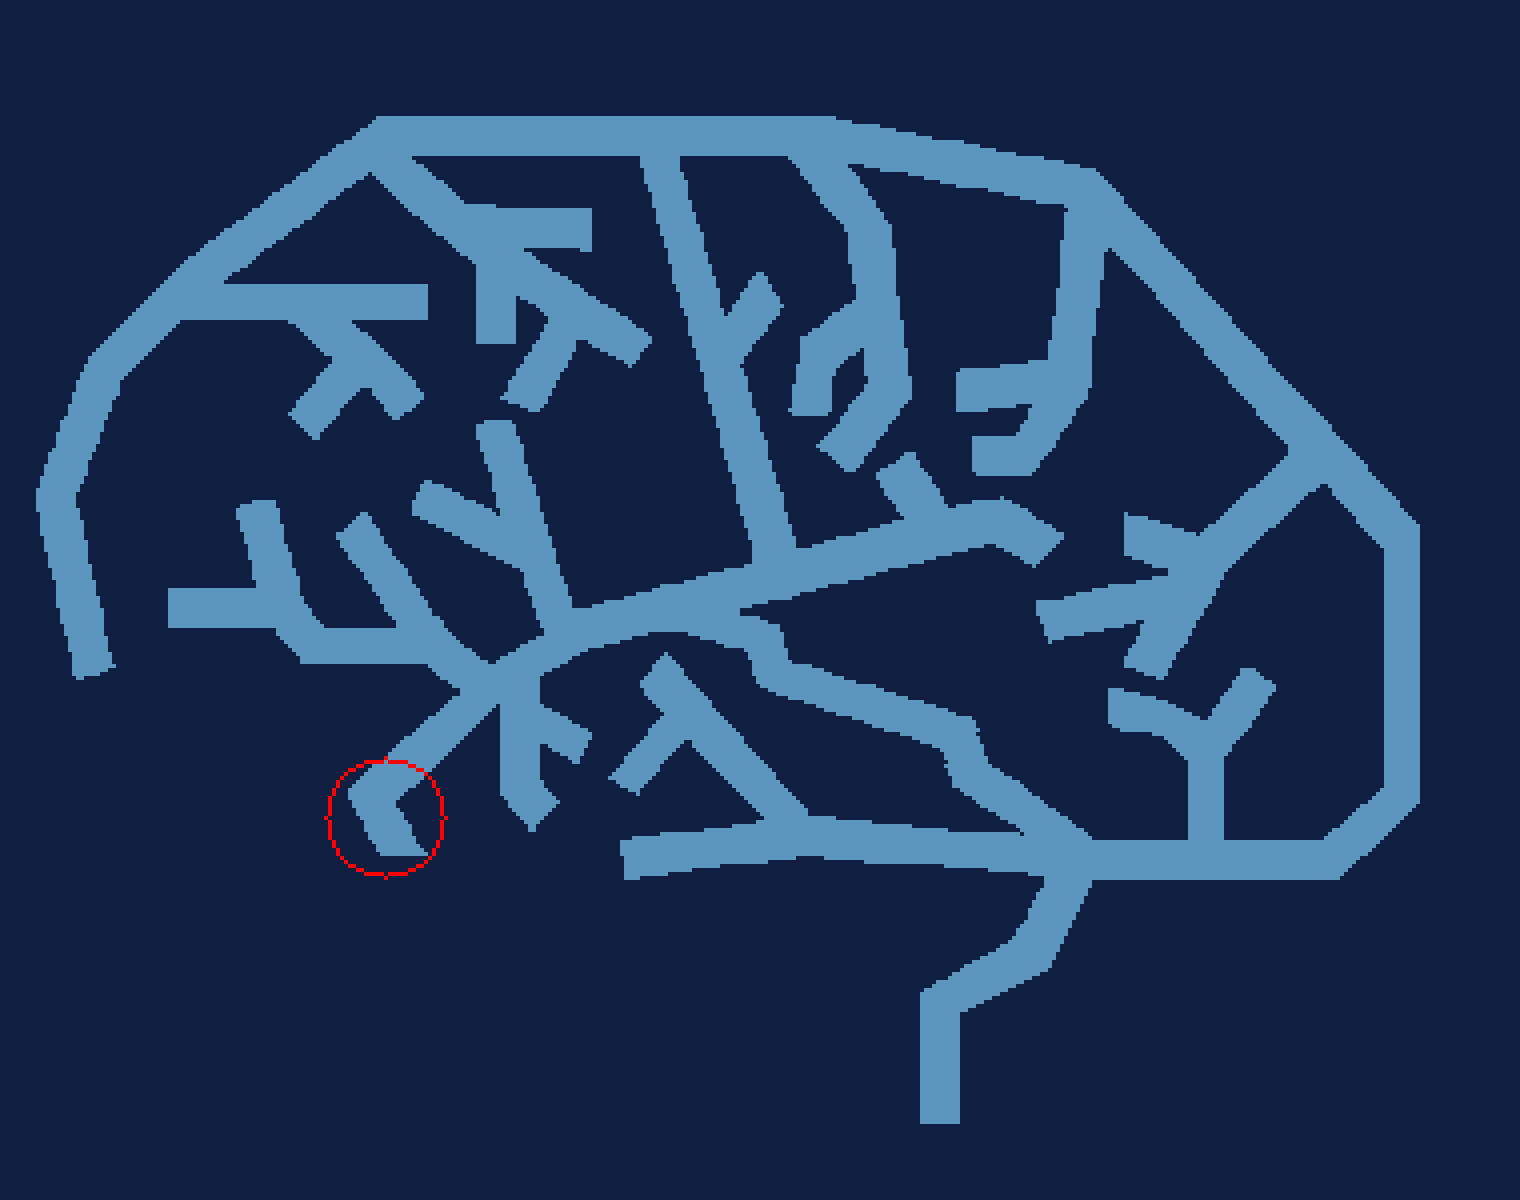
\includegraphics[clip, width=3.5cm]{figures/evaluation/procedure/brain_upscaled.png}} & Brain & $(380 \times 300)$ & $22593 \ (\approx 19.82\%)$ & 221.19 & 400 \\
            \addlinespace[0.05cm]
            \midrule
            
            \parbox[c]{3.5cm}{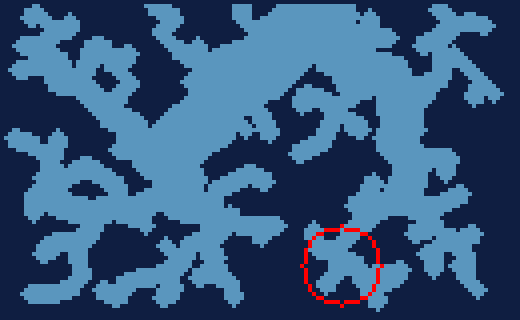
\includegraphics[clip, width=3.5cm]{figures/evaluation/procedure/vessel_upscaled.png}} & Vessel & $(130 \times 80)$ & $4949 \ (\approx 47.59\%)$ & 77.47 & 136 \\
            \addlinespace[0.05cm]
            \bottomrule
        \end{tabular}
    \end{center}
    \caption[Test Instances]{A list of our default test instances. Light blue pixels denote non-blocked pixels. The goal position is marked with a red circle. \textit{Dimension} describes the absolute size of the instance, while \textit{size} denotes the actual non-blocked area. We also included values for the average $d_{avg}$ and maximum $d_{max}$ distance between any point and the goal position.} \label{tab:TestInstances}
\end{table}

If not stated otherwise, we used 256 randomly generated particles for each episode during training. Episode lengths are capped at a maximum of 2000 steps independent of the environment. Dynamic episode lengths can also not exceed this hard cap.

\section{Reward Generation} \label{sec:EvalReward}
In this section we want to analyze how the reward generation influences training performance. In Section \ref{sec:RewardTestResults} we show our results and highlight key findings. We then continue to analyze some of the more important findings in Section \ref{sec:RewardAnalysis} and finish with our conclusion in Section \ref{sec:RewardConclusion}.

Since rewards are a key element to reinforcement learning, we expect that different rewards will heavily impact training performance. Our reward system provides a huge number of possible combinations of reward components and we therefore decide to use an iterative testing approach: We first test many combinations on the easy Corridor instance and then only evaluate the promising combinations on the Vessel instance. We finally select only the best performing combinations from the Vessel instance and test them on the Brain instance. Since observation normalization can have a huge impact on training performance and directly influences reward generation in the case of intrinsic reward, we also decided to add a second form of observation normalization in the form of $x \mapsto CLIP((x - \mu)/\sigma, [-10, 10])$ into this experiment. Note that the observation normalization of $x \mapsto x/255$ is always used if the second normalization option is not used.

Throughout this section we will provide a number of tables, which use abbreviations to save space. The abbreviations are explained in Table \ref{tab:RewardAbbreviations}.  

\begin{table} [ht]
    \begin{center}
        \small
        \begin{tabular}{ll}
            \toprule
            \multicolumn{1}{c}{Reward Component} & Abbreviation \\
            \midrule
            Continuous Reward & CR \\
            Discrete Reward & DR \\
            Observation Normalization & ON \\
            Reward Normalization & RN \\
            Time Penalty & TP \\
            Dynamic Episode Length & DEL \\
            Curiosity Reward & RND \\
            Gathering Reward & GR \\
            \bottomrule
        \end{tabular}
    \end{center}
    \caption[Abbreviations for Reward Components]{Common abbreviations for reward components} \label{tab:RewardAbbreviations}
\end{table}


\subsection{Test Results} \label{sec:RewardTestResults}

\paragraph{Corridor Environment.}
We begin with our easy instance Corridor. In our tests, we use the basic settings from Section \ref{sec:TestProcedure} and train for 3 million steps per trial. Table \ref{tab:Maze0318/Reward/Discrete} contains the results for discrete rewards and Table \ref{tab:Maze0318/Reward/Continuous} contains the results for continuous rewards.

Looking at the data, we can see, that many parameters do work very well and our dense discrete reward produces results which result in vastly shorter training times than in previous work \cite{huang2019}. Our initial experiments for discrete reward also show some interesting findings: 
\begin{itemize}
    \item \textbf{Normalization. } We found, that normalization has a huge impact on training performance. Normalizing the reward has a positive impact on its own (see Experiments 4/6), but additionally normalizing the observation by mean and standard deviation seems to be very important to improve performance in comparison to simple normalization (see Experiments 7/11 or 8/10).
    \item \textbf{Curiosity. } Using our relatively dense discrete reward, curiosity does not seem to have a positive effect for simple instances. Using DEL, a small amount of curiosity reward seems to have a positive impact (see Experiments 1/3), but also can have a negative impact if the weight is higher (see Experiments 1/2 or 13/14). Curiosity may have a greater impact when training with more complex instances though.
    \item \textbf{Dynamic Episode Length. } DEL does not seem to have any positive impact on the training performance. Experiment 9 shows that DEL is capable of creating time penalty like pressure, but the final result is worse than training with our normal time penalty. In combination with curiosity reward or a standard time penalty, performance seems to also worsen. (see Experiments 11/13; 12/14)
    \item \textbf{Gathering Reward. } Gathering reward does not seem to have any influence on the performance for small instances. Further testing will show, if this changes with larger or more challenging instances, where gathering of particles before bringing them to the goal might be more beneficial.
\end{itemize}


\begin{table}[htp]
    \begin{center}
        \begin{tabular}{rccccccrrr}
            \toprule
             & \multicolumn{6}{c}{Reward Component} & \multicolumn{2}{c}{Episode Length} & \\
            \cmidrule(lr){2-7}\cmidrule(lr){8-9}
            \multicolumn{1}{c}{Idx} & \multicolumn{1}{c}{ON} & \multicolumn{1}{c}{RN} & \multicolumn{1}{c}{TP} & \multicolumn{1}{c}{DEL} & \multicolumn{1}{c}{RND} & \multicolumn{1}{c}{GR} & \multicolumn{1}{c}{Best} & \multicolumn{1}{c}{Avg} & \multicolumn{1}{c}{Drop}\\
            \midrule
            1 &  &  &  & X &  &  & 256.78 & 295.04 & 1.25M \\
            2 &  &  &  & X & 0.50 &  & 499.97 & 499.99 & 750k \\
            3 &  &  &  & X & 0.25 &  & 110.94 & 117.82 & 750k \\
            4 &  &  & X &  &  &  & 135.03 & 145.34 & 629k \\
            5 &  &  & X &  & 0.25 &  & 324.29 & 422.48 & 456k \\
            6 &  &  & X & X &  &  & 477.62 & 491.48 & 3M \\
            7 &  & X & X &  &  &  & 83.78 & 84.66 & 461k \\
            8 &  & X & X &  &  & 1.00 & 93.31 & 94.30 & 406k \\
            9 & X & X &  & X &  &  & 65.72 & 67.17 & 400k \\
            10 & X & X & X &  &  & 1.00 & 59.31 & \textbf{65.68} & 190k \\
            11 & X & X & X &  &  &  & \textbf{57.38} & 66.81 & 182k \\
            12 & X & X & X &  & 0.50 &  & 84.52 & 207.78 & \textbf{181k} \\
            13 & X & X & X & X &  &  & 65.34 & 78.93 & 400k \\
            14 & X & X & X & X & 0.50 &  & 500.00 & 500.00 & 3M \\
            \bottomrule
        \end{tabular}
    \end{center}
    \caption[Evaluation of Discrete Reward Evaluation with the Corridor Environment]{Evaluation of discrete rewards with the corridor environment.} \label{tab:Maze0318/Reward/Discrete}
\end{table}


The evaluation results using continuous reward show similar outcomes to the experiments using discrete reward. The most important finding is, that the best continuous reward is able to produce superior results in every category compared to the best discrete reward. Especially the time of first notable improvement is about 30\% earlier. We included a plot showing the average episode length during training in Figure \ref{fig:ContinuousVsDiscrete}. This further supports our decision to create more dense rewards. 

\begin{table}[htp]
    \begin{center}
        \begin{tabular}{rccccccccrrr}
            \toprule
             & \multicolumn{8}{c}{Reward Component} & \multicolumn{2}{c}{Episode Length} & \\
            \cmidrule(lr){2-9}\cmidrule(lr){10-11}
            \multicolumn{1}{c}{Idx} & \multicolumn{1}{c}{ON} & \multicolumn{1}{c}{RN} & \multicolumn{1}{c}{TP} & \multicolumn{1}{c}{DEL} & \multicolumn{1}{c}{RND} & \multicolumn{1}{c}{GR} & \multicolumn{1}{c}{Int Norm} & \multicolumn{1}{c}{PO} & \multicolumn{1}{c}{Best} & \multicolumn{1}{c}{Avg} & \multicolumn{1}{c}{Drop}\\
            \midrule
            1 &  &  &  & X &  &  & X &  & 101.06 & 106.07 & 600k \\
            2 &  &  &  & X & 0.25 &  & X &  & 394.12 & 413.82 & 800k \\
            3 &  &  & X &  &  &  &  &  & 146.38 & 149.47 & 787k \\
            4 &  &  & X &  &  &  & X &  & 102.44 & 103.96 & 718k \\
            5 &  &  & X & X &  &  & X &  & 92.12 & 96.00 & 400k \\
            6 &  & X & X &  &  &  & X & X & 90.47 & 98.18 & 370k \\
            7 &  & X & X &  &  &  & X &  & 101.62 & 102.40 & 525k \\
            8 &  & X & X &  &  & 1.00 & X &  & 96.22 & 103.99 & 614k \\
            9 &  & X & X &  & 0.25 &  & X &  & 198.44 & 335.29 & 561k \\
            10 & X & X &  & X &  &  & X &  & 82.41 & 83.32 & 400k \\
            11 & X & X & X &  &  &  &  &  & \textbf{56.59} & \textbf{59.04} & \textbf{127k} \\
            12 & X & X & X &  &  &  & X & X & 58.72 & 65.46 & 152k \\
            13 & X & X & X &  &  &  & X &  & 61.81 & 71.28 & 147k \\
            14 & X & X & X &  &  & 1.00 &  &  & 60.53 & 62.46 & 149k \\
            15 & X & X & X &  &  & 1.00 & X &  & 59.09 & 68.69 & 151k \\
            16 & X & X & X &  & 0.25 &  & X & X & 69.41 & 246.38 & 158k \\
            17 & X & X & X & X &  &  & X & X & 79.19 & 79.39 & 400k \\
            \bottomrule
        \end{tabular}
    \end{center}
    \caption[Evaluation of Continuous Reward with the Corridor Environment]{Evaluation of continuous rewards with the corridor environment.} \label{tab:Maze0318/Reward/Continuous}
\end{table}


\begin{figure}[htp]
    
    \begin{center}
        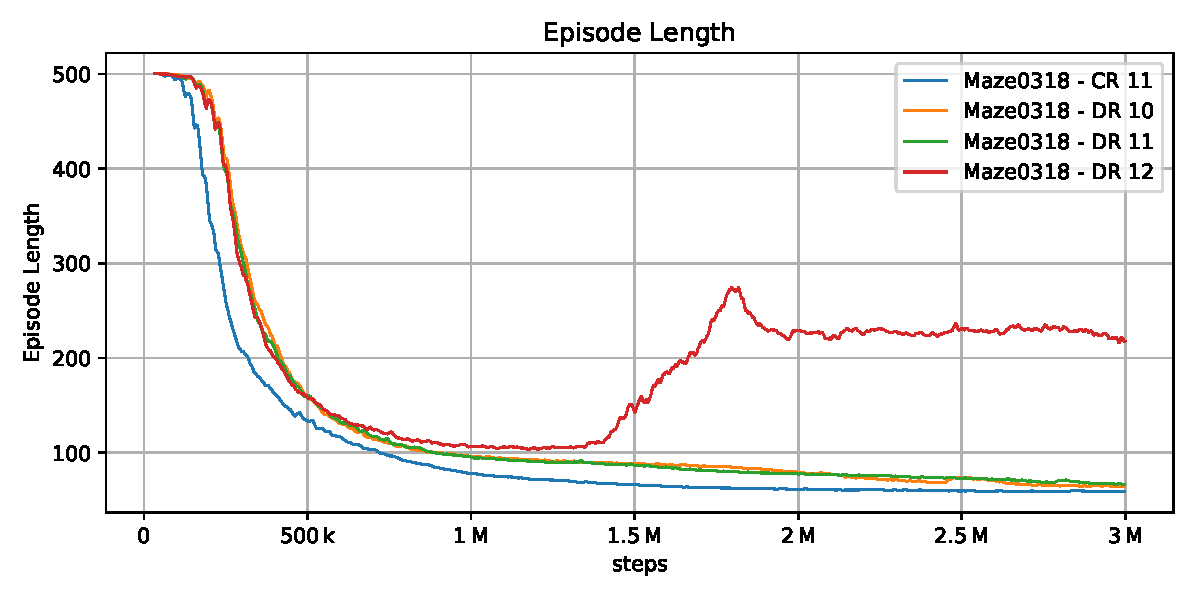
\includegraphics[clip, width=0.75\columnwidth]{figures/evaluation/rewards/continuous_vs_discrete.pdf}
    \end{center}
    
    %\vspace*{-6pt}
    \caption[Training Curves with Curiosity Reward]{Average episode length on the corridor environment during training. The legend refers to experiment numbers.}
    \label{fig:ContinuousVsDiscrete}
    %\vspace*{-12pt}
\end{figure}

\begin{figure}[htp]
    
    \begin{center}
        \begin{tabular}{c}
            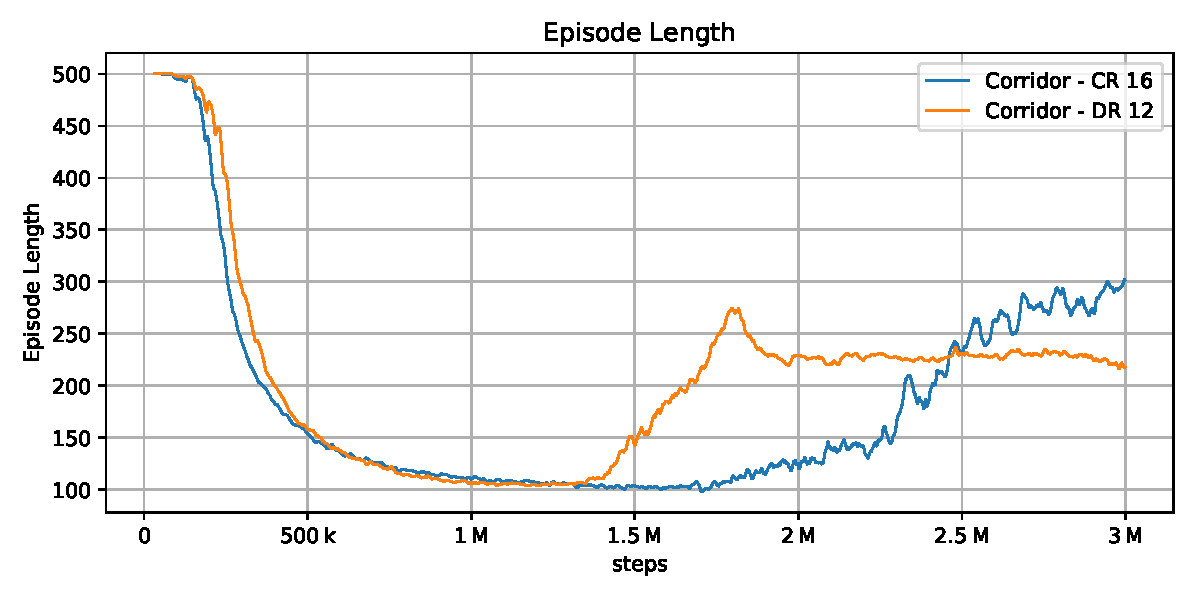
\includegraphics[clip, width=0.75\columnwidth]{figures/evaluation/rewards/curiosity_divergence_ep_len.pdf} \\
            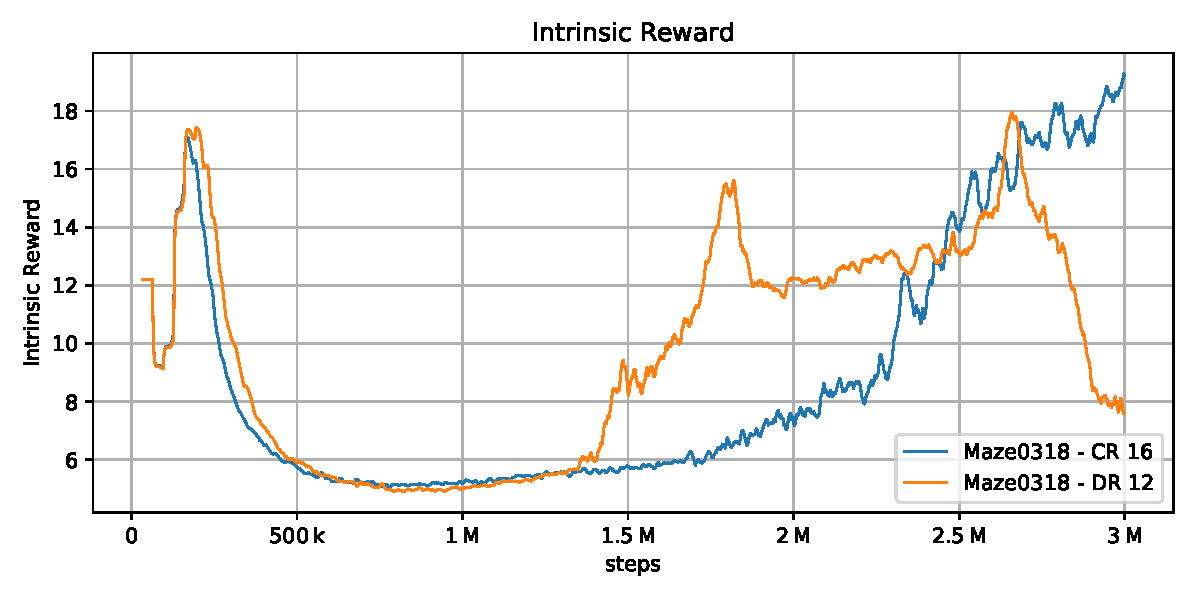
\includegraphics[clip, width=0.75\columnwidth]{figures/evaluation/rewards/curiosity_divergence_int_rew.pdf} \\
            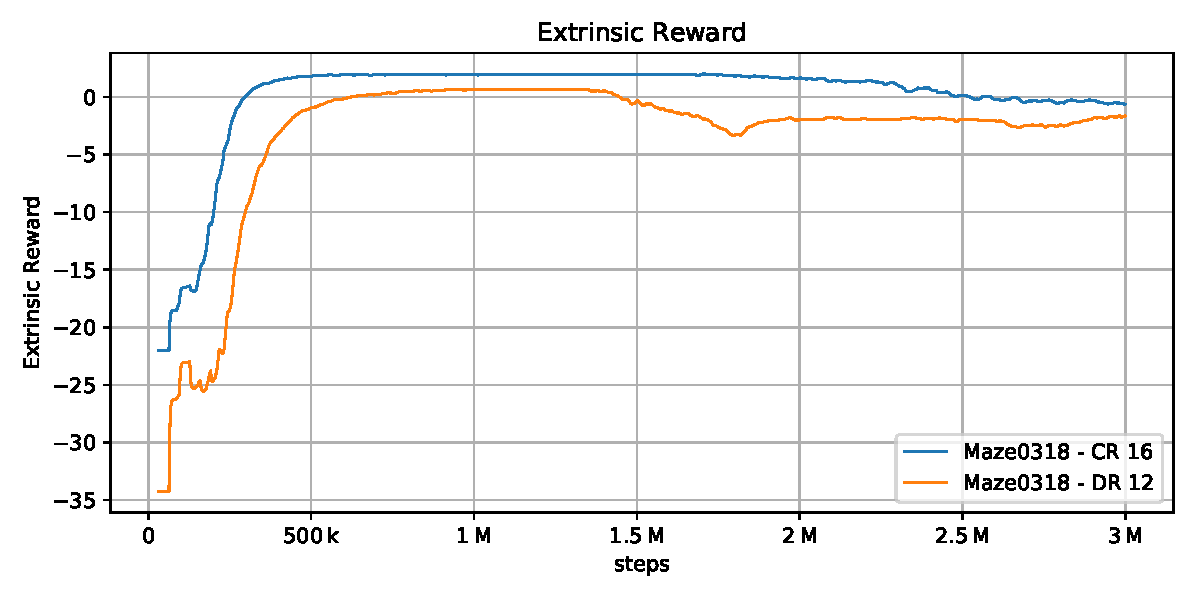
\includegraphics[clip, width=0.75\columnwidth]{figures/evaluation/rewards/curiosity_divergence_ext_rew.pdf}
        \end{tabular}

    \end{center}
    
    %\vspace*{-6pt}
    \caption[Problems with Curiosity Reward]{Learning curves for training with curiosity reward. We observed, that intrinsic rewards increase the chance for a performance collapse during training in terms of episode length. This can be seen, by comparing the intrinsic to the extrinsic reward and looking at the episode length at the same time: At around 1.5 million training steps, the intrinsic reward begins to increase, while the extrinsic reward remains at a constant level. At the same time, the average episode length begins to increase.}
    \label{fig:CuriosityDiverge}
    %\vspace*{-12pt}
\end{figure}


Similar to the results obtained when using discrete rewards, we can see, that observation normalization by mean and standard deviation massively improves performance for continuous rewards. Curiosity also does not seem to improve the results and often tends to diverge from the optimum at the end of training as shown in Figure \ref{fig:CuriosityDiverge}. Otherwise the corridor instance seems to be too easy to show differences between other reward parameters. Like before, gathering reward does not seem to have any positive or negative impact. The use of positive only rewards shows to improve performance without normalization (see Experiments 3/4), but only has a small impact with normalization (see Experiments 12/13). Interestingly internal normalization which balances the total cost reward against the maximum cost reward has shown to worsen the results on the corridor environment (see Experiments 11/13). 


\paragraph{Vessel Environment.} We repeat multiple experiments on the more complicated, but similarly large vessel instance. The results for discrete rewards are shown in Table \ref{tab:VesselMaze02/Reward/Discrete} and the results for continuous reward in Table \ref{tab:VesselMaze02/Reward/Continuous}. To compensate for the more complex environment, we double the training time for the agent and train for 6 millions steps per trial. 

Looking at the results for discrete rewards in Table \ref{tab:VesselMaze02/Reward/Discrete}, we can see, that normalization is crucial for success. While agents trained with non-normalized rewards are still able to find solutions, they need much more training time. For discrete rewards, the addition of a supporting reward signals seems to be important: The experiments including dynamic episode length (3), gathering reward (5) or curiosity reward (6) all produced better results, than stand-alone discrete reward (4). Especially the combination of discrete reward with curiosity was able to find a solution in a relatively short time. Note, that training with curiosity is significantly slower due to the extra computation for the training of the predictor network. 

\begin{table}[htp]
    \begin{center}
        \begin{tabular}{rccccccrrr}
            \toprule
             & \multicolumn{6}{c}{Reward Component} & \multicolumn{2}{c}{Episode Length} & \\
            \cmidrule(lr){2-7}\cmidrule(lr){8-9}
            \multicolumn{1}{c}{Idx} & \multicolumn{1}{c}{ON} & \multicolumn{1}{c}{RN} & \multicolumn{1}{c}{TP} & \multicolumn{1}{c}{DEL} & \multicolumn{1}{c}{RND} & \multicolumn{1}{c}{GR} & \multicolumn{1}{c}{Best} & \multicolumn{1}{c}{Avg} & \multicolumn{1}{c}{Drop}\\
            \midrule
            1 &  &  &  & X & 0.25 &  & 478.91 & 487.95 & 9.99M \\
            2 &  &  & X &  & 0.25 &  & 491.19 & 497.06 & 9.99M \\
            3 & X & X &  & X &  &  & \textbf{89.38} & 95.75 & 1.2M \\
            4 & X & X & X &  &  &  & 97.28 & 100.09 & 762k \\
            5 & X & X & X &  &  & 1.00 & 93.78 & \textbf{95.15} & 828k \\
            6 & X & X & X &  & 0.50 &  & 107.31 & 109.18 & \textbf{694k} \\
            7 & X & X & X & X &  &  & 89.62 & 96.38 & 1.2M \\
            \bottomrule
        \end{tabular}
    \end{center}
    \caption[Evaluation of Discrete Reward Evaluation with the Vessel Environment]{Evaluation of discrete rewards with the vessel environment.} \label{tab:VesselMaze02/Reward/Discrete}
\end{table}


The results for continuous rewards differ from the results for discrete rewards. By looking at Table \ref{tab:VesselMaze02/Reward/Continuous} we can see, that the addition of supporting rewards often produces worse results (see Experiments 7/11, 4/5, 8/10). An exception seems to be the combination of gathering reward with not internally normalized reward (see Experiments 6/9). Using only positive reward, does not seem to improve performance. The same is true for dynamic episode lengths.  


\begin{table}[htp]
    \begin{center}
        \begin{tabular}{rccccccccrrr}
            \toprule
             & \multicolumn{8}{c}{Reward Component} & \multicolumn{2}{c}{Episode Length} & \\
            \cmidrule(lr){2-9}\cmidrule(lr){10-11}
            \multicolumn{1}{c}{Idx} & \multicolumn{1}{c}{ON} & \multicolumn{1}{c}{RN} & \multicolumn{1}{c}{TP} & \multicolumn{1}{c}{DEL} & \multicolumn{1}{c}{RND} & \multicolumn{1}{c}{GR} & \multicolumn{1}{c}{Int Norm} & \multicolumn{1}{c}{PO} & \multicolumn{1}{c}{Best} & \multicolumn{1}{c}{Avg} & \multicolumn{1}{c}{Drop}\\
            \midrule
            1 &  &  & X &  & 0.25 &  & X &  & 451.00 & 476.26 & 7.92M \\
            2 &  & X & X &  &  &  &  &  & 423.09 & 433.16 & 7.81M \\
            3 &  & X & X &  &  &  & X & X & 373.28 & 405.12 & 8M \\
            4 &  & X & X &  &  &  & X &  & 416.28 & 458.89 & 7.91M \\
            5 &  & X & X &  &  & 1.00 & X &  & 418.75 & 470.94 & 7.05M \\
            6 & X & X & X &  &  &  &  &  & 93.97 & 98.73 & \textbf{501k} \\
            7 & X & X & X &  &  &  & X & X & 103.16 & 105.57 & 628k \\
            8 & X & X & X &  &  &  & X &  & 91.06 & \textbf{96.72} & 532k \\
            9 & X & X & X &  &  & 1.00 &  &  & \textbf{89.41} & 100.26 & 600k \\
            10 & X & X & X &  &  & 1.00 & X &  & 95.16 & 98.65 & 507k \\
            11 & X & X & X &  & 0.25 &  & X & X & 126.94 & 197.88 & 601k \\
            12 & X & X & X & X &  &  & X & X & 185.62 & 193.65 & 2.8M \\
            \bottomrule
        \end{tabular}
    \end{center}
    \caption[Evaluation of Continuous Reward with the Vessel Environment]{Evaluation of continuous rewards with the vessel environment.} \label{tab:VesselMaze02/Reward/Continuous}
\end{table}

\paragraph{Brain Environment.} We finally tested our the best performing reward configurations from the vessel environment on the brain environment. To compensate for the larger instance size and increased complexity, we again doubled training times, resulting in a total of 12 million training steps per trial. 

The results for discrete reward are listed in Table \ref{tab:Maze0122/Reward/Discrete}. Surprisingly, two of the three selected rewards did perform very poorly. Neither the configuration with dynamic episode length nor the one with curiosity reward did yield acceptable end results after 12 million training steps. The only discrete reward variation that can solve the brain environment successfully under the given time limit uses additional gathering reward. 


\begin{table}[htp]
    \begin{center}
        \begin{tabular}{rccccccrrr}
            \toprule
             & \multicolumn{6}{c}{Reward Component} & \multicolumn{2}{c}{Episode Length} & \\
            \cmidrule(lr){2-7}\cmidrule(lr){8-9}
            \multicolumn{1}{c}{Idx} & \multicolumn{1}{c}{ON} & \multicolumn{1}{c}{RN} & \multicolumn{1}{c}{TP} & \multicolumn{1}{c}{DEL} & \multicolumn{1}{c}{RND} & \multicolumn{1}{c}{GR} & \multicolumn{1}{c}{Best} & \multicolumn{1}{c}{Avg} & \multicolumn{1}{c}{Drop}\\
            \midrule
            1 & X & X &  & X &  &  & 500.00 & 500.00 & 12M \\
            2 & X & X & X &  &  & 1.00 & \textbf{311.44} & \textbf{319.23} & \textbf{7.15M} \\
            3 & X & X & X &  & 0.50 &  & 479.59 & 486.36 & 12M \\
            \bottomrule
        \end{tabular}
    \end{center}
    \caption[Evaluation of Discrete Reward with the Brain Environment]{Evaluation of discrete rewards with the brain environment.} \label{tab:Maze0122/Reward/Discrete}
\end{table}

In contrast to the discrete reward variations, all continuous reward configurations were able to solve the brain environment. As we can see from Table \ref{tab:Maze0122/Reward/Continuous}, the addition of gathering reward yields the best results, while internally normalized (balanced) continuous reward performs better than non-balanced reward.

\begin{table}[htp]
    \begin{center}
        \begin{tabular}{rccccccccrrr}
            \toprule
             & \multicolumn{8}{c}{Reward Component} & \multicolumn{2}{c}{Episode Length} & \\
            \cmidrule(lr){2-9}\cmidrule(lr){10-11}
            \multicolumn{1}{c}{Idx} & \multicolumn{1}{c}{ON} & \multicolumn{1}{c}{RN} & \multicolumn{1}{c}{TP} & \multicolumn{1}{c}{DEL} & \multicolumn{1}{c}{RND} & \multicolumn{1}{c}{GR} & \multicolumn{1}{c}{Int Norm} & \multicolumn{1}{c}{PO} & \multicolumn{1}{c}{Best} & \multicolumn{1}{c}{Avg} & \multicolumn{1}{c}{Drop}\\
            \midrule
            1 & X & X & X &  &  &  &  &  & 328.97 & 352.97 & 7.46M \\
            2 & X & X & X &  &  &  & X &  & \textbf{308.31} & 333.53 & 7.34M \\
            3 & X & X & X &  &  & 1.00 & X &  & 324.78 & \textbf{333.35} & \textbf{6.75M} \\
            \bottomrule
        \end{tabular}
    \end{center}
    \caption[Evaluation of Continuous Reward with the Brain Environment]{Evaluation of continuous rewards with the brain environment.} \label{tab:Maze0122/Reward/Continuous}
\end{table}


\subsection{Analysis} \label{sec:RewardAnalysis}
While it is easy to understand that dense rewards provide more information to the agent and thus produced superior results, other aspects are not as clear. In this section we want to analyze the learned behavior under different reward settings, to get a better understanding why certain configurations work better than others.

\paragraph{Curiosity.} Intrinsic reward has been the key to success for previous work, while our experiments showed a negative influence on training performance. To understand this, we analyzed how episodes are solved by agents trained with and without curiosity. In Figure \ref{fig:curiosity_ep_analysis} we show metrics taken at each step over the course of a single episode on the corridor environment. Both agents were trained using continuous reward, using the settings from Experiment 11 (without curiosity) and Experiment 16 (with curiosity) on the corridor environment. 

\begin{figure}[htp]
    \begin{center}
        \begin{tabular}{c}
            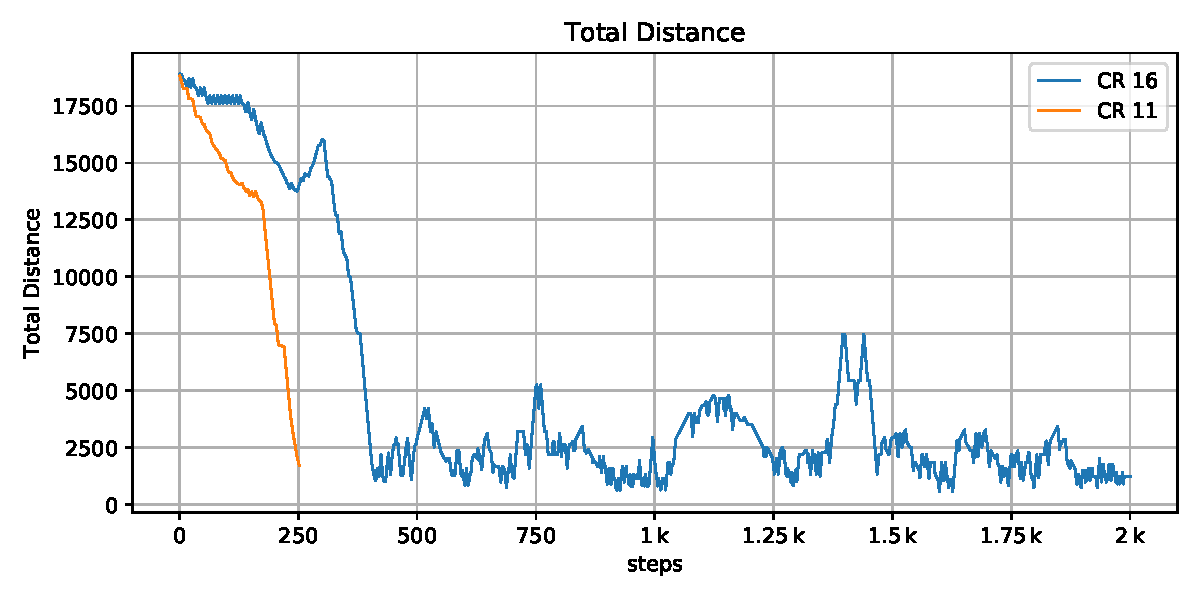
\includegraphics[clip, width=0.75\columnwidth]{figures/evaluation/rewards/episode_analysis/curiosity_total_distance.pdf} \\
            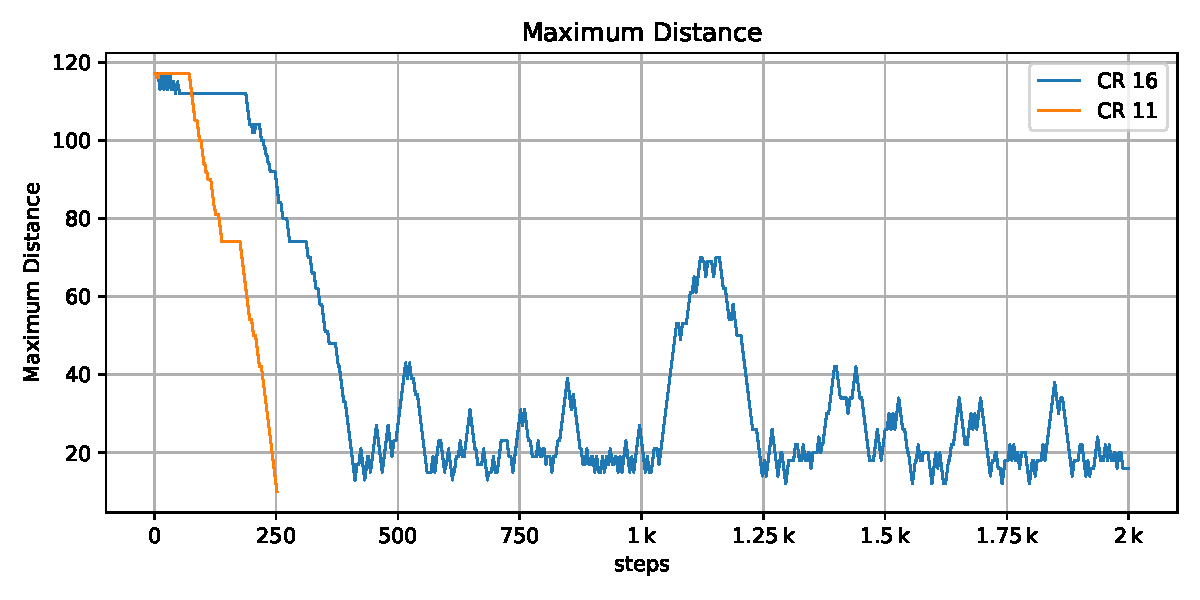
\includegraphics[clip, width=0.75\columnwidth]{figures/evaluation/rewards/episode_analysis/curiosity_max_distance.pdf} \\
            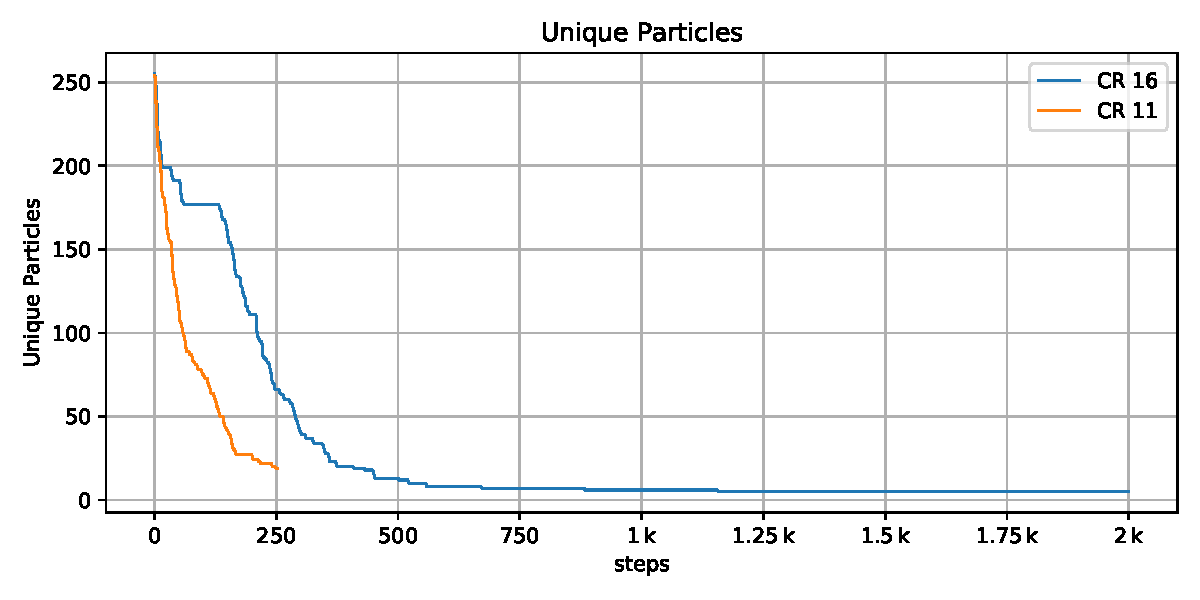
\includegraphics[clip, width=0.75\columnwidth]{figures/evaluation/rewards/episode_analysis/curiosity_unique_particles.pdf} \\
        \end{tabular}
    \end{center}
    \caption[Episode metrics on the Corridor Environment]{Metrics for a single example episode on the corridor instance. The steps are given without the MaxAndSkip wrapper and therefore in comparison 4 times larger. The blue line shows an agent trained with curiosity (see Experiment 16) and the orange line an agent trained without curiosity (see Experiment 11). The agent trained without curiosity is able to end the episode after about 250 steps, while the agent trained with curiosity does not end the episode during the 2000 steps time limit.} \label{fig:curiosity_ep_analysis}
\end{figure}


By looking at Figure \ref{fig:curiosity_ep_analysis} we can see, that both agents are able to reduce the total distance to the goal position very fast at the beginning of the episode. While the agent trained without curiosity finishes the episode after about 250 steps, the agent trained with curiosity decides to continue the episode by moving the particles back and forth close to the goal position. One could argue, that the agent might have to deal with a single particle that was left behind in the maze earlier, but this is not the case. We can see this by looking at the maximum distance any particle is away from the goal position. The particle which is the farthest away from the goal is closer than 20 pixels at around 470 steps and since the corridor environment only contains straight corridors, we can argue, that this particle cannot be stuck behind any obstacle. 

The question is why has the agent learned to not finish the episode when training with curiosity? We found, that there is a number of reasons why curiosity reward can be maximized by not finishing the episode. Let us begin with the easiest one: In Section \ref{sec:blRND} we showed, that an agent trained purely with curiosity learns to maximize episode lengths. Since it is able to explore more states during longer episodes, it can generate more intrinsic reward, if episodes are longer. The same happens in our particle environment where short episodes result in less intrinsic reward. Curiosity therefore works against our goal of achieving short episodes lengths. 

Another problem with curiosity comes from the nature of how the observations are generated in our environment: Since particles are directly shown in the observation and there are a lot of particles at the same time, the agent has control over a decent number of its own observation inputs. Since the agent is able to rapidly move the particles to appear at different positions, it is able to generate a massive amount of environment states and therefore observations similar to input noise. This situation is directly related to the \textit{noisy tv problem} described by Burda et al. \cite{burda2018large}. We can directly see this behavior in Figure \ref{fig:curiosity_ep_analysis}, where the agent has learned to increase the number of states, by gradually moving the particles to and away from the goal position, while slowly reducing the number of unique particles. Unfortunately this problem is not easy to fix. Implementing a large goal reward, may increase the number of episodes where the agent actually brings all particles to the goal, but the agent can still finish the episode at the last possible moment. Increasing the time penalty was found to help to some extend during our initial experiments. Previous experiments \cite{huang2019,becker2020} also used a larger time penalty and therefore may have not encountered this problem. Unfortunately we found that increasing the time penalty requires very careful fine-tuning for each environment to work correctly and therefore does not fix the underlying problem.

\paragraph{Observation Normalization. } Throughout our experiments, we observed large benefits from changing the observation normalization from normalization to the interval [0, 1] to normalization which also centers around zero by normalizing by $x \mapsto CLIP((x - \mu)/\sigma, [-10, 10])$. While normalization itself is a common technique in machine learning and has shown to improve training (e.g. \cite{jayalakshmi2011statistical}), for image-based tasks the normalization by mean and standard deviation is often used to compensate for brightness variation while still scaling the images to a smaller interval \cite{pal2016preprocessing}. 

In our case brightness variation is irrelevant, because our images are generated by our environment and do not change in brightness. So why does the agent still benefit from this normalization type? Because the area which is blocked by the maze never changes in value, when subtracting the mean from the input observation, the input becomes zero in all places where the maze blocks pixels. This makes it easier for the agent to ignore areas where no particles can be, because zero values in the input always mean zero activations in the network. Learning that an input value has no meaning is a harder task. The second reason is a benefit for the backpropagation algorithm, which works more stable, if it can work with zero centered input, since it allows the gradients to be both positive and negative.

\paragraph{Strategies.}
One interesting aspect for the future choice of rewards would be, if the learned strategies differ depending on the given reward. Looking at the change of total distance to the goal position in the brain environment (see Figure \ref{fig:Rewards/Ep_Analysis}), we can assume, that the learned strategies are pretty similar. Except for agents trained with the discrete reward in combination with DEL or curiosity, the change in distances is very similar.  

\begin{figure}[htp]
    \begin{center}
        \begin{tabular}{c}
            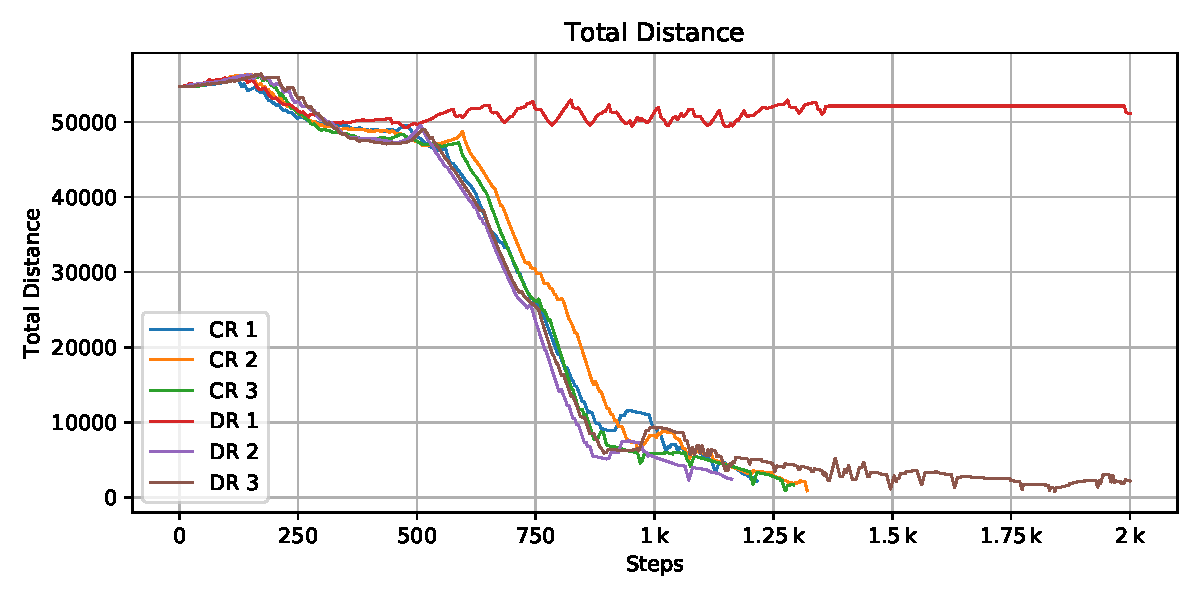
\includegraphics[clip, width=0.95\columnwidth]{figures/evaluation/rewards/episode_analysis/maze0122_total_dist.pdf} \\
            \includegraphics[clip, width=0.95\columnwidth]{figures/evaluation/rewards/episode_analysis/maze0122_total_dist_avg.pdf} \\
        \end{tabular}
    \end{center}
    \caption[Episode metrics on the Brain Environment]{Total sum of distances to the goal position over a single episode on the brain environment. On the top, we included a plot showing a single episode and on the bottom we included the average over 64 episodes.} \label{fig:Rewards/Ep_Analysis}
\end{figure}

To verify this result we monitor the similarity between actions for a given observation. We generate trajectories by replaying the different agents on the brain environment. We then replay the observations to all agents and count the differences in the choice of the best action (using stochastic policies). Note that an alternative measure would be to calculate an approximate Kullback-Leibler distance using the generated trajectories, but we found, that results are hard to interpret.

\begin{table}[htp]
    \begin{center}
        \begin{threeparttable}
            \begin{tabular}{l|rrrrrrr}
                \toprule
                vs & DR 2 & DR 2\tnote{1} & DR 3 & DR 1 & CR 2 & CR 3 & CR 1 \\
                \midrule
                DR 2 & 100.00 & 50.09 & 37.25 & 15.19 & 42.31 & 44.79 & 42.31 \\
                DR 2\tnote{1} & 50.09 & 100.00 & 45.41 & 10.89 & 39.33 & 43.84 & 45.83 \\
                DR 3 & 37.25 & 45.41 & 100.00 & 13.12 & 34.69 & 36.73 & 39.75 \\
                DR 1 & 15.19 & 10.89 & 13.12 & 100.00 & 15.68 & 18.43 & 15.10 \\
                CR 2 & 42.31 & 39.33 & 34.69 & 15.68 & 100.00 & 45.19 & 50.73 \\
                CR 3 & 44.79 & 43.84 & 36.73 & 18.43 & 45.19 & 100.00 & 48.54 \\
                CR 1 & 42.31 & 45.83 & 39.75 & 15.10 & 50.73 & 48.54 & 100.00 \\
                \bottomrule
            \end{tabular}
            \begin{tablenotes} \footnotesize
                \item[1] This agent uses the same reward as DR2, but from a different trial.
            \end{tablenotes}
        \end{threeparttable}
    \end{center}
    \caption[Agent Action Similarity for Different Rewards]{Similarity of actions between different agents given in percent of equal actions for the same observation on the brain environment. Similarity is measured by first generating observations by replaying the agents and then comparing the actions different agents would have chosen in the same situation.} \label{tab:Maze0122/Reward/Similarity}
\end{table}

We included the results in terms of percent of equal actions for the same observations in Table \ref{tab:Maze0122/Reward/Similarity}. A surprising result is, that two agents trained with the \textit{same} reward only produce the same action for about 50\% of the observations. The most reasonable explanation is that we have a set with very similar actions (e.g. NE, N, NW) and there are many situations where either of these actions can be used. Different neural networks then evolved into using only one of them for a specific input and therefore produce very dissimilar results for the same observation, even when trained with the same reward. Keeping this baseline in mind, we can see, that agents trained with different rewards also differ in their percentage of equal actions. Most notably the both worst performing agents trained with discrete reward (DR 1 and DR 3). For all other agents, the differences are significantly smaller. We can observe, that the agents using internally normalized (CR 2) and not internally normalized reward (CR 1) essentially learned the same strategy since they agree on even more observations than the two agents trained with DR 2. Adding gathering reward seems to lead to a slightly different strategy with between 2 and 5 percent of different action choices. 

Overall the choices of all agents which also yield good performance are relatively close. We can therefore assume, that the learned strategies only differ slightly and the agents all evolved into learning an similar optimized strategy independent of the used reward. 

\subsection{Conclusion} \label{sec:RewardConclusion}
When deciding for a reward for our further experiments, we have to keep in mind, that every extra computation will be executed for each individual training step. The more reward components we use, the longer training will take. When comparing the results on the brain environment for continuous reward, we saw that the addition of gathering reward just slightly improves the average end result. If we look at the wall-clock time, a single trial on the brain environment using the gathering reward took an average of 4:54h to complete, while a trial using only the continuous reward took 4:27h on average. This means that with gathering reward, we saw an increase of about 10\% more time. While additional components might provide benefits for special environments (see Section \ref{sec:EvalRandomness}) they do not provide significant improvements for our general case. Depending on the environment size, multiple rewards can be used to achieve good performance, but only a few scale well into larger instances. We therefore will use continuous internally normalized reward for all further experiments.

\section{RL Algorithms} \label{sec:EvalRLAlgorithms}
In this section we want to evaluate how different RL algorithms perform when solving maze environments. We presented a number of algorithms in Chapter \ref{chp: RLOverview} and want to test some of the most recent approaches including DQN (see Section \ref{ssec:DeepQLearning}), PPO (see Section \ref{ssec:PPO}), ACER and ACKTR (see Section \ref{ssec:AlternativeCombinedMethods}). Since the performance of most RL algorithms is very sensitive to the chosen hyperparameters, we optimized the parameters for each individual algorithm on the Vessel instance. This optimization included a wide range of parameters which were preselected using our automated hyperparametersearch system. We then used manual fine-tuning to get an optimal configuration for each algorithm. 

The parameters we selected for DQN, ACER and ACKTR can be found in Table \ref{tab:RLHyperparameters}. For PPO, we found that the parameters we choose during our initial experiments were already suited to yield good results and we will therefore use the parameters given in Table \ref{tab:PPOHyperparemeters}. PPO was also found to work with a wide range of parameters, e.g. increasing the number of optimization epochs could yield faster initial results, but is very time-consuming. We also tried to increase the number of parallel environments, but found that this does not further improve performance.  Decreasing the number of steps also has a positive initial effect, but worsens the final result.

\begin{table}[htp]
    \begin{center}
        \begin{threeparttable}
            \begin{tabular}{c}
                \begin{tabular}{|m{6cm}|R{2.5cm}|}
                    \hline
                    \multicolumn{1}{|c|}{Hyperparameter} & \multicolumn{1}{c|}{Value} \\
                    \hline
                    Rollout Length & 16 \\
                    Buffer Size & 5000 \\
                    Entropy Coefficient & 0.0001 \\
                    $\gamma$ & 0.98 \\
                    Learning Rate & 0.0007 \\
                    Learning Rate Schedule & Linear \\
                    Optimization Algorithm & RMSProp \cite{tieleman2012lecture} \\
                    Q Coefficient & 0.6 \\
                    Replay Ratio & 4 \\
                    Replay Start & 1000 \\
                    \hline
                \end{tabular} \\
                \addlinespace[0.15cm]
                {\small (a) Hyperparameters for ACER} \\
                \addlinespace[0.5cm]
                \begin{tabular}{|m{6cm}|R{2.5cm}|}
                    \hline
                    \multicolumn{1}{|c|}{Hyperparameter} & \multicolumn{1}{c|}{Value} \\
                    \hline
                    Rollout Length & 32 \\
                    Entropy Coefficient & 0.01 \\
                    $\gamma$ & 0.99 \\
                    $\lambda$ & 0.99 \\
                    Learning Rate & 0.2 \\
                    Value Function Coefficient & 0.25 \\
                    \hline
                \end{tabular} \\
                \addlinespace[0.15cm]
                {\small (b) Hyperparameters for ACKTR} \\
                \addlinespace[0.5cm]
                \begin{tabular}{|m{6cm}|R{2.5cm}|}
                    \hline
                    \multicolumn{1}{|c|}{Hyperparameter} & \multicolumn{1}{c|}{Value} \\
                    \hline
                    Learning Rate & 0.0005 \\
                    Learning Starts & 1000 \\
                    Target Network Update Frequency & 1000 \\
                    Train Frequency & 4 \\
                    Exploration Fraction & 0.5 \\
                    Exploration Final Epsilon & 0.05 \\
                    Buffer Size & 150000 \\
                    Prioritized Replay $\alpha$ & 0.6 \\
                    Prioritized Replay $\beta$ & 0.4 \\
                    \hline
                \end{tabular} \\
                \addlinespace[0.15cm]
                {\small (c) Hyperparameters for DQN\tnote{1} \ \tnote{2}} \\
    
            \end{tabular}
            \begin{tablenotes} \footnotesize
                \item[1] The DQN implementation of stable-baselines uses Double DQN and Dueling DQN.
                \item[2] We removed frame stacking and observation normalization for DQN as we found that it worsens results.
            \end{tablenotes}
        \end{threeparttable}
        
    \end{center}
    \caption[Hyperparameters]{Hyperparameters used for different RL Algorithms.} \label{tab:RLHyperparameters}
\end{table}

\subsection{Results}

Similar to previous experiments we tested the RL algorithms on our three test instances. The results for the Corridor instance can be found in Table \ref{tab:AlgorithmEval/Maze0318}, the results for the Vessel instance in Table \ref{tab:AlgorithmEval/VesselMaze02} and the results for the Brain instance in Table \ref{tab:AlgorithmEval/Maze0122}. Looking at the data, we can see, that three of our four algorithms performed well during the tests, namely ACER, ACKTR and PPO. DQN failed to deliver results even for the smallest instance and also took very long for each trial.

\begin{table}[htp]
    \begin{center}
        \begin{tabular}{rcrrrrr}
            \toprule
            \multicolumn{1}{c}{Idx} & \multicolumn{1}{c}{Algorithm} & \multicolumn{1}{c}{Best} & \multicolumn{1}{c}{Avg} & \multicolumn{1}{c}{Drop} & \multicolumn{1}{c}{Time}\\
            \midrule
            1 & PPO & 61.81 & 71.28 & 147k & 0:40:36h \\
            2 & DQN & 500.00 & 500.00 & 381k & 3:08:00h \\
            3 & ACKTR & 63.38 & 70.73 & 424k & \textbf{0:32:49h} \\
            4 & ACER & \textbf{55.84} & \textbf{68.83} & \textbf{100k} & 0:41:40h \\
            \bottomrule
        \end{tabular}
    \end{center}
    \caption[Evaluation of RL Algorithms on the Corridor Instance]{Evaluation results for different RL algorithms on the Corridor instance. We can see that ACER produced the best end results while also providing a fast initial improvement. In terms of wall-clock time, ACKTR provided the fastest results. DQN failed to solve the instance during our model evaluation episodes, but was able to solve some episodes during training (therefore the drop is below 3M).} \label{tab:AlgorithmEval/Maze0318}
\end{table}

\begin{table}[htp]
    \begin{center}
        \begin{tabular}{rcrrrrr}
            \toprule
            \multicolumn{1}{c}{Idx} & \multicolumn{1}{c}{Algorithm} & \multicolumn{1}{c}{Best} & \multicolumn{1}{c}{Avg} & \multicolumn{1}{c}{Drop} & \multicolumn{1}{c}{Time}\\
            \midrule
            1 & PPO & \textbf{91.06} & \textbf{96.72} & 532k & 1:10:00h \\
            2 & DQN & 500.00 & 500.00 & 6M & 5:40:24h \\
            3 & ACKTR & 103.88 & 109.20 & 759k & \textbf{0:51:54h} \\
            4 & ACER & 111.72 & 117.50 & \textbf{182k} & 1:12:57h \\
            \bottomrule
        \end{tabular}
    \end{center}
    \caption[Evaluation of RL Algorithms on the Vessel Instance]{Evaluation results for different RL algorithms on the Vessel instance. PPO is able to train the best performing agent, while ACKTR produces the fastest training times and ACER provides the fastest initial improvement. DQN again fails to deliver usable results.} \label{tab:AlgorithmEval/VesselMaze02}
\end{table}

\begin{table}[htp]
    \begin{center}
        \begin{tabular}{rcrrrrr}
            \toprule
            \multicolumn{1}{c}{Idx} & \multicolumn{1}{c}{Algorithm} & \multicolumn{1}{c}{Best} & \multicolumn{1}{c}{Avg} & \multicolumn{1}{c}{Drop} &  \multicolumn{1}{c}{Time}\\
            \midrule
            1 & PPO & \textbf{308.31} & \textbf{333.53} & \textbf{7.34M} & \textbf{4:28:39h} \\
            2 & ACKTR & 341.78 & 367.42 & 9.12M & 4:32:15h \\
            3 & ACER & 500.00 & 500.00 & 12M & 4:51:40h \\
            \bottomrule
        \end{tabular}
    \end{center}
    \caption{Evaluation results for different RL algorithms on the Brain instance. PPO delivers the best results in all categories (bold), delivering the best results in the shortest time. ACER fails to solve larger instances and may need more time or specific fine-tuning.} \label{tab:AlgorithmEval/Maze0122}
\end{table}

When comparing the other algorithms, we an see, that they all show certain strengths and weaknesses. ACER is able to provide very good results on the small Corridor instance, while also being the fastest in terms of initial improvement on both the Corridor and the Vessel instance. However ACER fails to solve the larger and more complex Brain instance during 12 million steps of training. ACKTR only provides average end results, while the algorithm is surprisingly fast in terms of wall-clock time. PPO shows to have the best overall performance, delivering the best results on the Vessel and Brain instance while still maintaining a reasonably good performance in terms of speed.   

\subsection{Analysis}
A surprising result for our experiments is that DQN was not able to solve even the easiest instance Corridor. Looking at the average episode length during training (see Figure \ref{fig:Algorithm/Ep_Length}) we see, that DQN was able to solve the environment at multiple points during training, but suffered from multiple training collapses. Interestingly the network trained with DQN was not able to solve the environment at test time during training. This means, that the DQN agent always relied on certain randomness coming from the epsilon-greedy strategy to randomly solve the maze. Because there exist a lot more DQN extensions which especially improve exploration, we suggest that a more powerful implementation of DQN might yield better results in the future.

\begin{figure}[htp]
    \begin{center}
        \begin{tabular}{c}
            \includegraphics[clip, width=0.75\columnwidth]{figures/evaluation/algorithms/maze0318_episode_length.pdf} \\
            {\small (a) Episode length of different RL algorithms on the Corridor instance} \\
            \includegraphics[clip, width=0.75\columnwidth]{figures/evaluation/algorithms/vesselmaze02_episode_length.pdf} \\
            {\small (b) Episode length of different RL algorithms on the Vessel instance} \\
            \includegraphics[clip, width=0.75\columnwidth]{figures/evaluation/algorithms/maze0122_episode_length.pdf} \\
            {\small (c) Episode length of different RL algorithms on the Brain instance} \\
        \end{tabular}
    \end{center}
    \caption[Episode Length During Training on the Test Environment]{Average episode length during training on our three test environments. We can see, that DQN is able to solve the easier instances at some point, but later suffers from training collapses. ACER is able to make very fast progress on Corridor and Vessel, but fails to solve Brain. PPO and ACKTR both solve all instances, with PPO delivering superior results in a smaller number of steps.} \label{fig:Algorithm/Ep_Length}
\end{figure}

\paragraph{Training Progress}
Figure \ref{fig:Algorithm/Ep_Length} shows the average episode length during training with different RL algorithms for our three test instances. Looking at Figure \ref{fig:Algorithm/Ep_Length} (a), we can see that DQN was able to compute solutions at various points during training, but suffered from performance collapses multiple times and was therefore unable to converge to a good final solution. All other algorithms were able to compute good solutions during the first one million training steps and then slowly optimized their results. 

\begin{figure} [htp]
    \begin{center}
        \begin{tabular}{c}
            \begin{tabular}{ccc}
                \includegraphics[width=0.26\columnwidth]{figures/evaluation/algorithms/training_example/acktr/0_k.png} & 
                \includegraphics[width=0.26\columnwidth]{figures/evaluation/algorithms/training_example/acktr/6_k.png} & 
                \includegraphics[width=0.26\columnwidth]{figures/evaluation/algorithms/training_example/acktr/12_k.png} \\
                \addlinespace[0.2cm]
                \includegraphics[width=0.26\columnwidth]{figures/evaluation/algorithms/training_example/acktr/18_k.png} &
                \includegraphics[width=0.26\columnwidth]{figures/evaluation/algorithms/training_example/acktr/25_k.png} & 
                \includegraphics[width=0.26\columnwidth]{figures/evaluation/algorithms/training_example/acktr/29_k.png} \\
            \end{tabular} \\
            \addlinespace[0.1cm]
            {\small (a) Images from the first episode of training.} \\
            \addlinespace[0.5cm]
            \begin{tabular}{ccc}
                \includegraphics[width=0.26\columnwidth]{figures/evaluation/algorithms/training_example/acktr/30_k.png} & 
                \includegraphics[width=0.26\columnwidth]{figures/evaluation/algorithms/training_example/acktr/37_k.png} & 
                \includegraphics[width=0.26\columnwidth]{figures/evaluation/algorithms/training_example/acktr/44_k.png} \\
                \addlinespace[0.2cm]
                \includegraphics[width=0.26\columnwidth]{figures/evaluation/algorithms/training_example/acktr/51_k.png} &
                \includegraphics[width=0.26\columnwidth]{figures/evaluation/algorithms/training_example/acktr/58_k.png} & 
                \includegraphics[width=0.26\columnwidth]{figures/evaluation/algorithms/training_example/acktr/65_k.png} \\
            \end{tabular} \\
            \addlinespace[0.1cm]
            {\small (b) Images from the second episode of training.} \\
        \end{tabular}
    \end{center}
    \caption[Images During Training Episodes with ACKTR]{Images from the first two episodes of training using ACKTR (from one of the 64 parallel environments). ACKTR improves the strategy of the agent each 32 steps, changing it about 15 times during a single episode. The first episode (a) is largely dominated by the random actions of the new neural network, but still delivers the particles to the goal, because ACKTR quickly favors actions moving particles down and \textit{later} actions moving particles right. The second episode (b) includes the knowledge from the first episode, but moving particles to the right too early leads to particles getting stuck in the corridor above the bottom corridor.} \label{fig:AcktrTrainingEpisodes}
\end{figure}


Looking at the training curve for ACKTR we can see a surprising unexpected result at the beginning of the training process: The average episode length is below the threshold of 500 steps at the beginning of training and then rises back to the maximum, before it drops again at around 500 thousand steps into training. To explain this anomaly, we included a series of images in Figure \ref{fig:AcktrTrainingEpisodes}, showing frames from the initial episodes generated during training. Figure \ref{fig:AcktrTrainingEpisodes} (a) shows images from the very first episode during training. The ACKTR agent trains its network every 32 steps, improving the network several times over the course of one episode. Because the network is only trained for a short time and stochastic actions are used during training, the agent is able to solve some of the 64 parallel environments, by quickly learning to choose actions that move particles downwards and later more actions which move particles to the right. After finishing the episode the agent learned, that going down and right somehow maximizes its reward and repeats this process. Unfortunately, going to the right too early brings particles into a place, where they are stuck and can only be moved to the goal, by going left (see Figure \ref{fig:AcktrTrainingEpisodes} (b)). Because this is the opposite of what the agent learned so far and it does not directly generate positive reward, due to other particles being moved away from the goal, the agent then struggles to learn this new behavior for the next few episodes.

Figure \ref{fig:Algorithm/Ep_Length} (b) and (c) show the average episode length during training for the Vessel and Brain environment. We can see that ACER optimizes faster for smaller instances, but fails to perform on the larger Brain instance. The curves for PPO and ACKTR seem to be pretty similar, with PPO always delivering results in less steps than ACKTR. This is most probably because the ACKTR implementation does not support the usage of multiple optimization epochs and is therefore less sample efficient than the PPO implementation. 

\begin{figure} [htp]
    \begin{center}
        \includegraphics[width=0.45\columnwidth]{figures/evaluation/algorithms/training_example/vessel/vessel_problems.png}
    \end{center}
    \caption[Training Challenges in the Vessel Environment]{Training challenges in the Vessel environment. After 100k training steps, all algorithms tend to already deliver a decent number of particles to the goal position. The rest of the training then is focused on learning movements to also bring particles to the goal which get stuck in the process and often require movements which bring particles away from the goal position. We highlighted spots where particles often get stuck in \textit{orange}.} \label{fig:Algorithm/Problems/Vessel}
\end{figure}


\begin{figure} [htp]
    \begin{center}
        \begin{tabular}{cc}
            \multicolumn{2}{c}{\includegraphics[width=0.45\columnwidth]{figures/evaluation/algorithms/training_example/brain/brain_first_progress.png}} \\
            \multicolumn{2}{c}{\small (a) Initial Problems}\\
            \addlinespace[0.5cm]
            \includegraphics[width=0.45\columnwidth]{figures/evaluation/algorithms/training_example/brain/brain_problem_1.png} & 
            \includegraphics[width=0.45\columnwidth]{figures/evaluation/algorithms/training_example/brain/brain_problem_2.png} \\
            {\small (b) Strategy after the first 3M Training Steps} & {\small (c) Final Strategy}\\
        \end{tabular}
    \end{center}
    \caption[Training Challenges in the Brain environment]{Training challenges in the Brain environment. Algorithms learn to gather particles at the position marked in green after 100k training steps (a). During this gathering process a number of particles gets stuck at the positions marked in orange. After the first 3 million training steps (see (b)), the strategy is complex enough, to retrieve most of the particles and gather them in the area marked in green. While moving the particles down, a number of particles gets stuck at the top (orange). Other particles are stuck at the bottom the whole time. After a few more million training steps, the agent changes its strategy and gathers particles at the top (not only in the corner) (see (c)). Particles are then gathered in an area near the top right corner and brought down to the goal. Particles stuck at the orange positions are retrieved when the particles from the top are already close to the goal.} \label{fig:Algorithm/Problems/Brain}
\end{figure}

After analyzing how ACKTR struggled with the Corridor environment, we also wanted to highlight problems all agents had when training on the Vessel or Brain environment. In Figure \ref{fig:Algorithm/Problems/Vessel} we highlighted the areas where particles got stuck after the first 100k training steps in orange. These places are not surprising, since particles stuck at these positions require movements which would increase the distance to the goal for most of the other particles. We can see from Figure \ref{fig:Algorithm/Ep_Length} (b) that all algorithms except DQN figure out a way to retrieve most of these particles in less than 2 million steps of training. Finally Figure \ref{fig:Algorithm/Problems/Brain} shows us problematic regions for training on the Brain environment. We again highlighted spots, where particles get stuck in orange. The algorithms initially learn to gather particles in the area highlighted in green (see Figure \ref{fig:Algorithm/Problems/Brain} (a)) and then learn to bring the particles closer to the goal via the path highlighted in green in Figure \ref{fig:Algorithm/Problems/Brain} (b). Some particles then often get stuck in the path close to the right of the path to the goal (highlighted in orange). The algorithm then learn an improved strategy over time, which gathers particles at the top without further gathering them in the top left corner, and then gather particles in the top right corner before moving them down to the goal (see Figure \ref{fig:Algorithm/Problems/Brain} (c)). Particles at the bottom will be retrieved later, once particles from the top are already close to the goal. As we can see from Figure \ref{fig:Algorithm/Ep_Length} all algorithms need far more time to solve the Brain environment. The question that remains is if the Brain environment is harder to solve because of its structure, or because of its size. We will leave this question open for future work.

\paragraph{Result Variation}
When it comes to comparing results, we always have to keep in mind, that the execution of neural networks with Tensorflow 1.14 is not deterministic and we therefore have to deal with a certain amount of result variation. All our experiments so far were therefore repeated three times and we always compared the average results. For future experiments it might be beneficial to know how much this nondeterminism influences our results using different RL algorithms.

\begin{table}[htp]
    \begin{center}
        \begin{threeparttable}
            \begin{tabular}{crrrrrr}
                \toprule
                 & \multicolumn{2}{c}{Corridor} & \multicolumn{2}{c}{Vessel} & \multicolumn{2}{c}{Brain} \\
                \cmidrule(lr){2-3} \cmidrule(lr){4-5} \cmidrule(lr){6-7}
                \multicolumn{1}{c}{Algorithm} & \multicolumn{1}{c}{CV} & \multicolumn{1}{c}{Delta} & \multicolumn{1}{c}{CV} & \multicolumn{1}{c}{Delta} & \multicolumn{1}{c}{CV} & \multicolumn{1}{c}{Delta} \\
                \midrule
                PPO & 9.40\% & 14.56 & 4.32\% & 9.97 & 8.47\% & 64.66\\
                ACKTR & \textbf{7.59\%} & \textbf{12.66} & \textbf{3.55\%} & \textbf{9.09} & \textbf{4.98\%} & \textbf{41.53} \\
                ACER & 13.36\% & 20.06 & 3.86\% & 11.09 & - & - \\
                \midrule
                PPO\tnote{1} & 7.11\% & 10.81 & 4.74\% & 10.89 & 5.53\% & 44.58 \\
                \bottomrule
            \end{tabular}
            \begin{tablenotes}
                \footnotesize
                \item[1] Results are calculated as an average over data from the reward experiments, excluding experiments using DEL, curiosity or no normalization.
            \end{tablenotes}

        \end{threeparttable}
        
    \end{center}
    \caption[Result Variation Using Different RL Algorithms]{Result variation in terms of final episode length during evaluation in absolute numbers (difference between maximum and minimum) and as coefficient of variation (CV) ($\sigma / \mu$) on the three test instances. ACKTR seems to produce the most stable results due to its improved optimization technique, while PPO and ACER still produce comparable results. The variation seems to increase for larger instances. Note that the sample size for the upper part of this table is fairly low with only three repetitions per experiment. We therefore included a second row for PPO using data from the reward experiments for comparison.} \label{tab:Algorithm/ResultVariation}
\end{table}

We start by looking at the variation during the experiments for the different RL algorithms as listed in Table \ref{tab:Algorithm/ResultVariation}. We can see, that ACKTR provides the most stable results, which is most likely due to its improved optimization technique. We can also see, that both ACER and PPO produce results with more variance, but still do limit the variance to a certain degree. We can therefore argue, that larger changes in performance due to some change in the experimental setup can still be detected, even when only using a single trial to compare results. 

Because the data we use is very limited due to each experiment being only repeated three times, the error in Table \ref{tab:Algorithm/ResultVariation} can be quite large. We therefore also analyze the variation in past experiments. Using data from the reward experiments with continuous reward and excluding experiments with DEL, curiosity reward or without normalization. Using this data, we can compute the result variation as an average over 15 trials for Corridor and Vessel and 9 trials for Brain. The results are shown in the last row of Table \ref{tab:Algorithm/ResultVariation}. We can see, that even with a larger sample size, we get comparable results. In praxis this means, that independent of the training randomness, we will still get a usable result at the end of the training process. For our experiments, results of single trials are comparable within a certain error bound, but evaluation of close results still requires multiple trials.

\subsection{Conclusion}
In this section we tested four popular RL algorithms - DQN, ACKTR, ACER and PPO - to solve our three test environments. We saw, that both ACKTR and PPO performed fairly well on all three environments, while DQN fails to solve even the easy Corridor environment. ACER was able to solve both the Corridor and the Vessel environment, but failed at the larger Brain environment. Since PPO is much more popular than ACKTR and also delivered slightly better results, we will continue to use PPO for all future experiments. 


\section{Observations} \label{sec:EvalObs}
All agents we trained so far used the same observation input: The environment generates an images containing the maze and all particle positions which is then downscaled to 84 by 84 pixels and stacked together with the previous four observations. This procedure is used by many other authors (e.g. \cite{burda2018large, mnih2015human}) and has shown to improve learning on the Atari benchmark. However all these games provide the exact same input dimensions with a screen being 160 pixels wide and 210 pixels high \cite{bellemare2013arcade}. Most of the games also include moving objects which are not under the direct control of the player, or include some sort of physics simulation with makes frame stacking very important to give the agent the possibility to estimate motion. For our simple particle environments, the input sizes are directly dependent on the size of the maze. This may require less downscaling for larger instances and may allow more downscaling for smaller ones. We will therefore analyze how much downscaling affects the results in Section \ref{sec:Eval/ObsSize}. While frame stacking is important if objects are moving without the player control, or the behavior of objects under the players control may depend on past states, our particle environment contains none of these two aspects. We therefore analyze, how agents behave under different levels of frame stacking in Section \ref{sec:Eval/FrameStack}.


\subsection{Observation Size} \label{sec:Eval/ObsSize}
Until now, we always trained our agents with the same observation size independent of the instance size. Surprisingly, we had no problems to train the agent, even on our largest instance which is over 10 times larger than our smallest instance. In this section we want to analyze how different input sizes affect learning on the same instance. 

Because observation size does not seem to matter to much in terms of performance, we also want to evaluate, if the agent is able to solve an instance without any input at all. This means that the agent will only receive a single input in form of a step counter. This counter gets incremented by 1 after each agent-environment interaction. Since the goal is static, the agent should be able to remember a sequence of movements which brings all (or most) particles to the goal position. Since we only have a single input, we have to change the network architecture for these experiments. All experiments which work with input size 1 use a fully connected network with three layers. The first two layers are shared between the actor and the critic and contain 512 and 1024 neurons respectively. The network then diverges and contains another fully connected layer with 256 neurons for each the actor and the critic.

\begin{table}[htp]
    \begin{center}
        \begin{threeparttable}
            \begin{tabular}{c}
                \begin{tabular}{rcrrrr}
                    \toprule
                    \multicolumn{1}{c}{Idx} & \multicolumn{1}{c}{Frame Size} & \multicolumn{1}{c}{Best} & \multicolumn{1}{c}{Avg} & \multicolumn{1}{c}{Drop} & \multicolumn{1}{c}{Time}\\
                    \midrule
                    1 & (100, 100) & \textbf{60.75} & \textbf{65.57} & 157k & 1:00:46h \\
                    2 & (84, 84) & 61.81 & 71.28 & \textbf{147k} & 0:40:36h \\
                    3 & (44, 44) & 78.00 & 79.42 & 181k & 0:21:17h \\
                    4 & (24, 24) & 82.28 & 84.67 & 209k & 0:22:12h \\
                    5 & (12, 12) & 500.00 & 500.00 & 1.41M & 0:15:19h \\
                    6 & (-, -) & 307.50 & 307.51 & 251k & \textbf{0:11:06h} \\
                    \bottomrule
                \end{tabular} \\
                \addlinespace[0.15cm]
                {\small (a) Results for the Corridor instance} \\
                \addlinespace[0.5cm]
                \begin{tabular}{rcrrrr}
                    \toprule
                    \multicolumn{1}{c}{Idx} & \multicolumn{1}{c}{Frame Size} & \multicolumn{1}{c}{Best} & \multicolumn{1}{c}{Avg} & \multicolumn{1}{c}{Drop} & \multicolumn{1}{c}{Time}\\
                    \midrule
                    1 & (130, 80) & 98.38 & 100.20 & 539k & 2:03:17h \\
                    2 & (84, 84) & \textbf{91.06} & \textbf{96.72} & 532k & 1:10:00h \\
                    3 & (44, 44) & 105.03 & 112.49 & 566k & 0:43:36h \\
                    4 & (24, 24) & 99.38 & 107.81 & \textbf{501k} & 0:45:29h \\
                    5 & (12, 12) & 494.75 & 495.42 & 6M & 0:31:24h \\
                    6 & (-, -) & 500.00 & 500.00 & 6M & \textbf{0:22:28h} \\
                    \bottomrule
                \end{tabular} \\
                \addlinespace[0.15cm]
                {\small (b) Results for the Vessel Instance} \\
                \addlinespace[0.5cm]
                \begin{tabular}{rcrrrr}
                    \toprule
                    \multicolumn{1}{c}{Idx} & \multicolumn{1}{c}{Frame Size} & \multicolumn{1}{c}{Best} & \multicolumn{1}{c}{Avg} & \multicolumn{1}{c}{Drop} & \multicolumn{1}{c}{Time}\\
                    \midrule
                    1\tnote{1} & (168, 168) & 356.47 & 356.47\tnote{1} & \textbf{6.22M} & 17:49:36h \\
                    2 & (84, 84) & \textbf{308.31} & \textbf{333.53} & 7.34M & 4:28:39h \\
                    3 & (44, 44) & 500.00 & 500.00 & 12M & 3:06:27h \\
                    4 & (24, 24) & 500.00 & 500.00 & 12M & 2:54:06h \\
                    5 & (-, -) & 500.00 & 500.00 & 12M & \textbf{0:49:34h} \\
                    \bottomrule
                \end{tabular} \\
                \addlinespace[0.15cm]
                {\small (c) Results for the Brain instance. We excluded results without} \\
                {\small any downsizing due to the massive increase in training time.} \\
                %\addlinespace[0.25cm]
            \end{tabular}
            \begin{tablenotes}
                \footnotesize
                \item[1] Due to the increase in training time we only performed a single trial for this experiment.
            \end{tablenotes}
        \end{threeparttable}
    \end{center}
    \caption[Training Results for Different Observation Sizes]{Training results with different observation sizes. (-, -) denotes only a single observation in the form of a step counter.} \label{tab:ObsSize}
\end{table}

Similar to before, we executed the experiments on our three standard instances. We use a wrapper to scale down the input and successively halve the frame size in both dimensions. We then round the size to match the neural network cnn architecture. For the smallest frame sizes $(24 \times 24)$ and $(12 \times 12)$ we have to remove the first convolutional layer of our network to work correctly. Otherwise the network is the same independent of the input.

\begin{figure}[htp]
    \begin{center}
        \includegraphics[clip, width=0.95\columnwidth]{figures/evaluation/observations/maze0318_ep_len_time.pdf}
    \end{center}
    \caption[Episode Length on the Corridor Environment using Different Observation Sizes]{Average episode length during training with different observation sizes on the corridor environment. The x-axis shows wall-clock time instead of steps to show effective performance.} \label{fig:ObsSize/Maze0318/EpLen}
\end{figure}


The results of our experiments can be found in Table \ref{tab:ObsSize}. We begin by looking at the results from the Corridor instance in Table \ref{tab:ObsSize} (a). We can see, that the agent is able to tolerate much lower observation sizes than 84 by 84. Even at a frame size of 24 by 24 (which is only about 8\% of the original input information) the agent is still able to solve the environment with only slightly worse performance. Interestingly the smaller frame size of 12 by 12 pixels is not sufficient to train the agent, while only a step counter as an observation is. We suspect that strong downscaling leads to many similar or even equal environment states even when particles are at very different locations, while the step counter input provides a clear distinction between states and therefore works better.

Different frame sizes do not only affect the performance of the learned strategy, but also have a great effect on wall-clock time. Figure \ref{fig:ObsSize/Maze0318/EpLen} shows the performance of the agents trained with different observation sizes in relation to time instead of steps. The time difference between input sizes does increase the larger the input gets. This is non surprising since the neural network needs to be larger and we therefore need to process more data. Due to hardware-related limitations this change in time is linear, but rather changes suddenly at certain points.

Let us now look at the results for the other instances in Table \ref{tab:ObsSize} (b) and (c). We can see, that even though the results were similar, there are some important differences: Even for slightly larger instances like the vessel instance, providing a larger input requires a change in network architecture to deal with the increased information. For both the vessel and the brain instance, increasing the observation size lead to much slower \textit{and} worse overall results. We will therefore try to improve the network to handle larger input sizes in Section \ref{sec:EvalNetworks}. Another important finding is, that we cannot simply downscale much larger instances and still expect good results. On the Brain instance the original 84 by 84 downscale was the tiniest observation size that still worked. This exposes a problem if we want to solve real-world instances which would be much larger or even three-dimensional. 


\subsection{Frame Stacking} \label{sec:Eval/FrameStack}
Frame stacking is important for settings where the agent must be able to estimate the movements of objects. For example if we want to drive a car and have top-down images of its position, we need to estimate its current velocity from its change of position, to calculate future movements. However in our particle environment, the movements of the particles will not be affected by past actions, since the particles do not have an internal velocity and stop after each move. We therefore expect frame stacking to only have a minor effect on the training process.   

\begin{table}[htp]
    \begin{center}
        \begin{tabular}{c}
            \begin{tabular}{rcrrrr}
                \toprule
                \multicolumn{1}{c}{Idx} & \multicolumn{1}{c}{Frame Stack} & \multicolumn{1}{c}{Best} & \multicolumn{1}{c}{Avg} & \multicolumn{1}{c}{Drop} & \multicolumn{1}{c}{Time}\\
                \midrule
                1 & 6 & 61.34 & 66.34 & 143k & 1:17:40h \\
                2 & 4 & 61.81 & 71.28 & 147k & 0:40:36h \\
                3 & 2 & 57.22 & 66.69 & 145k & 0:34:00h \\
                4 & 1 & \textbf{56.44} & \textbf{59.70} & \textbf{122k} & \textbf{0:31:25h} \\
                \bottomrule
            \end{tabular} \\
            \addlinespace[0.15cm]
            {\small (a) Results for the Corridor instance.} \\
            \addlinespace[0.5cm]
            \begin{tabular}{rcrrrr}
                \toprule
                \multicolumn{1}{c}{Idx} & \multicolumn{1}{c}{Frame Stack} & \multicolumn{1}{c}{Best} & \multicolumn{1}{c}{Avg} & \multicolumn{1}{c}{Drop} & \multicolumn{1}{c}{Time}\\
                \midrule
                1 & 6 & 107.91 & 108.86 & 569k & 2:02:54h \\
                2 & 4 & \textbf{91.06} & 96.72 & 532k & 1:10:00h \\
                3 & 2 & 92.06 & 99.84 & 443k & 0:59:14h \\
                4 & 1 & 93.16 & \textbf{94.32} & \textbf{382k} & \textbf{0:53:57h} \\
                \bottomrule
            \end{tabular} \\
            \addlinespace[0.15cm]
            {\small (b) Results for the Vessel Instance} \\
            \addlinespace[0.5cm]
            \begin{tabular}{rcrrrr}
                \toprule
                \multicolumn{1}{c}{Idx} & \multicolumn{1}{c}{Frame Stack} & \multicolumn{1}{c}{Best} & \multicolumn{1}{c}{Avg} & \multicolumn{1}{c}{Drop} & \multicolumn{1}{c}{Time}\\
                \midrule
                1 & 4 & \textbf{308.31} & \textbf{333.53} & 7.34M & 4:28:39h \\
                2 & 2 & 331.44 & 353.35 & 6.56M & 3:58:53h \\
                3 & 1 & 326.06 & 345.49 & \textbf{6.54M} & \textbf{3:49:05h} \\
                \bottomrule
            \end{tabular} \\
            \addlinespace[0.15cm]
            {\small (c) Results for the Brain Instance} \\
        \end{tabular}
        
    \end{center}
    \caption[Evaluation Results for Different Levels of Frame Stacking]{Results for different levels of frame stacking. The best values are marked in bold. We can see, that frame stacking does not improve learning for the basic maze environments. By disabling frame stacking (setting it to one) learning times can be significantly reduced (see (a)). Agents also learn better strategies on smaller instances using only single frames as input (see (a) bold). However this advantage does not seem to translate to larger instances (see (c)). We can argue, that the difference in performance is small enough, that the reduced training time compensates for the slightly worse performance. Without frame stacking, agents generally learn faster as they require both less steps (earlier drop time) and less computation time per step. The reduced computation time mainly originates from smaller neural networks due to the decreased input size. For (c) this difference is smaller, because the larger instance leads to a CPU instead of a GPU bottleneck.} \label{tab:Eval/FrameStacking}
\end{table}

We evaluated the effects of frame stacking on our three test instances and included the results  in Table \ref{tab:Eval/FrameStacking}. We can see, that our initial prediction was partially right and frame stacking does not seem to provide great benefits for training on our basic maze environments. Form Table \ref{tab:Eval/FrameStacking} (a) we can see, that removing frame stacking provides results in less overall time and also improves the final performance of the model for smaller instances. Unfortunately, this advantage seems to disappear for larger instances with longer training times (see Table \ref{tab:Eval/FrameStacking} (b) and (c)). By looking at Figure \ref{fig:Eval/FrameStacking/Maze0122} we can also see, that removing frame stacking may introduce more variance and training instability. 

Nevertheless, with less or no frame stacking we usually get comparably good results. Agents generally seem to learn faster, because the agent has to process and "understand" less information and therefore has to deal with less total states. As the agent does not need to know the position of particles over time, it can concentrate on the current position of the particles. The reduced input size also leads to smaller neural networks, which further accelerates learning in terms of wall-clock time. This can also be seen in Figure \ref{fig:Eval/FrameStacking/Maze0122} where we show the average episode length during training in relation to the training time. 

\begin{figure}[htp]
    \begin{center}
        \includegraphics[clip, width=0.8\columnwidth]{figures/evaluation/observations/maze0122_frame_stack_ep_len.pdf}
    \end{center}
    \caption[Average Training Episode Length for Different Levels of Frame Stacking]{Average episode length during training for different levels of frame stacking. The x-axis shows wall-clock time for training sessions of 12 million steps. We can see, that less frame stacking improves learning speed, but introduces more training instability.} \label{fig:Eval/FrameStacking/Maze0122}
\end{figure}

\paragraph{Conclusion. } Following our results, when training agents for the simple maze environment, we can remove frame stacking without loosing any performance. However we have to be careful with this decision when extending or changing the setting. For noisy observations (see Section \ref{sec:EvalError}) as well as when dealing with particles which keep their velocity (see Section \ref{sec:EvalPhysical}) it might be a significant disadvantage to remove this information. 


\section{Network Architecture} \label{sec:EvalNetworks}
In this section we want to evaluate how much influence different network architecture has on the performance. For all past experiments we used the same neural network structure, using a simple CNN equal to the one used in previous experiments. In Section \ref{sec:Eval/NetworkStructure}, we will test other networks on our test instances, to see, if we can achieve an improvement in training time or final result by adding or removing layers. Finally, we will also evaluate if we are able to improve the performance, by replacing the leaky ReLU activation function in Section \ref{sec:Eval/ActivationFunctions}.

\subsection{Network Structure} \label{sec:Eval/NetworkStructure}
The CNN we used in past experiments consists of three convolutional layers with 32 ($8 \times 8, s=2$), 64 ($4\times4, s=2$) and 64 ($4 \times 4, s=1$) filters respectively, followed by a single fully connected layer with 512 neurons. This network structure is widely used and has shown to provide good performance on tasks like the Atari benchmark (e.g. \cite{burda2018large, burda2018exploration, mnih2015human}). We therefore expect the CNN to be fairly optimized for the given input and mostly focus on the structure of the fully connected layers. We also expect network sizes to only matter for larger, more complicated instances, where more complex behavior has to be learned. We therefore limit our tests to the Vessel and the Brain instance.

\begin{table}[htp]
    \begin{center}
        \begin{threeparttable}
            \begin{tabular}{rccrrrr}
                \toprule
                \multicolumn{1}{c}{Idx} & \multicolumn{1}{c}{CNN} & \multicolumn{1}{c}{MLP} & \multicolumn{1}{c}{Best} & \multicolumn{1}{c}{Avg} & \multicolumn{1}{c}{Drop} & \multicolumn{1}{c}{Time}\\
                \midrule
                1 & default\tnote{1} & [128] & 101.97 & 104.03 & 476k & 1:09:56h \\
                2 & default\tnote{1} & [256] & 94.16 & 98.81 & 506k & \textbf{1:09:27h} \\
                3 & default\tnote{1} & [512] & \textbf{91.06} & \textbf{96.72} & 532k & 1:10:00h \\
                4 & default\tnote{1} & [512, 512] & 95.97 & 99.09 & 508k & 1:10:34h \\
                5 & default\tnote{1} & [512, {'pi': [512], 'vf': [512]}] & 101.03 & 104.18 & 538k & 1:10:47h \\
                6 & default\tnote{1} & [256, 448, {'pi': [448], 'vf': [448]}] & 98.38 & 107.02 & 536k & 1:10:37h \\
                7\tnote{2} & modified\tnote{3} & [512] & 110.00 & 114.35 & \textbf{413k} & 1:51:27h \\
                \bottomrule
            \end{tabular}
            \begin{tablenotes} \footnotesize
                \item[1] Structure: ('conv', 32, 8, 4), ('conv', 64, 4, 2), ('conv', 64, 3, 1)
                \item[2] We removed downscaling for this experiment.
                \item[3] Structure: ('conv', 32, 8, 4), ('pool', 2, 2), ('conv', 64, 4, 2), ('conv', 64, 3, 1)
            \end{tablenotes}

        \end{threeparttable}
        
    \end{center}
    \caption[Test Results for Different Network Structures on the Vessel Environment]{Test results for different network structures on the Vessel environment. The best results are marked in bold. We can see, that our initial network with 512 neurons in the dense layer provides the best results in terms of final result, while only performing very slightly slower than smaller networks on our test machine.} \label{tab:Eval/NetworkStructure/Vessel}
\end{table}

\begin{table}[htp]
    \begin{center}
        \begin{threeparttable}
            \begin{tabular}{rccrrrr}
                \toprule
                \multicolumn{1}{c}{Idx} & \multicolumn{1}{c}{CNN} & \multicolumn{1}{c}{MLP} & \multicolumn{1}{c}{Best} & \multicolumn{1}{c}{Avg} & \multicolumn{1}{c}{Drop} & \multicolumn{1}{c}{Time}\\
                \midrule
                1 & default\tnote{1} & [512] & \textbf{308.31} & 333.53 & 7.34M & 4:28:39h \\
                2 & default\tnote{1} & [512, {'pi': [512], 'vf': [512]}] & 317.84 & 334.83 & \textbf{6.79M} & \textbf{4:24:58h} \\
                3\tnote{2,3} & modified\tnote{4} & [512] & 326.53 & \textbf{326.53}\tnote{3} & 7.41M & 16:08:57h \\
                \bottomrule
            \end{tabular}
            \begin{tablenotes} \footnotesize
                \item[1] Structure: ('conv', 32, 8, 4), ('conv', 64, 4, 2), ('conv', 64, 3, 1)
                \item[2] We changed downscaling to ($168 \times 168$) for this experiment.
                \item[3] Due to the increase in training time, this experiment does not use multiple trials. 
                \item[4] Structure: ('conv', 32, 8, 4), ('pool', 2, 2), ('conv', 64, 4, 2), ('conv', 64, 3, 1)
            \end{tablenotes}
        \end{threeparttable}
    \end{center}
    \caption[Test Results for Different Network Structures on the Brain Environment]{Test results for different network structures on the Brain environment. Similarity to the test results on the Vessel environment (see Table \ref{tab:Eval/NetworkStructure/Vessel}) we can observe, that larger networks do not provide noticeable advantages or disadvantages. Increased size - especially in the convolutional layers - may lead to vastly increased training times though.} \label{tab:Eval/NetworkStructure/Brain}
\end{table}

Table \ref{tab:Eval/NetworkStructure/Vessel} shows the results for different network sizes on the Vessel instance. Surprisingly, we can see that the network structure does not seem to have a great impact on training performance. While the network we used for all past experiments provided the best results in terms of final performance, the performance of other network types was very similar. Even with only one quarter of the neurons in the fully connected layer the network still is able to perform well (see Experiment 1). Larger networks do not seem to benefit training neither in initial speed, nor in final performance (see Experiments 4, 5, 6). We also tried to increase the amount of information the network receives, by removing downscaling wrapper and compensating for the increased layer size by adding a max-pooling layer after the first convolution. Looking at the results for Experiment 7, we can see, that this change also does not benefit training and also increases training time drastically due to the increased size of the first convolutional filters. 

To verify our results, we also tested some of the networks on the larger Brain instance. The results are listed in Table \ref{tab:Eval/NetworkStructure/Brain}. The results are very similar to the results on the Vessel instance. Larger networks do not seem to provide an advantage in terms of final performance, but contrary to before, we can observe that the larger network in Experiment 2 seems to learn a little bit faster initially. 

\paragraph{Analysis. } The results from the experiments for different network structures are surprising, as neural networks are at the core of the RL agent. For single target goals, the size of the network does not seem to matter too much, as long as the CNN extractor retains its structure. Because the goal position does not change, the initial position of particles does not influence the required actions to bring the particles to the goal too much. The agents therefore do not need to learn very complex behavior and smaller networks are sufficient to learn this information. We perform additional experiments with random goals in Section \ref{sec:EvalRandomGoals} which support this claim.

\subsection{Activation Functions} \label{sec:Eval/ActivationFunctions}
In this section we want to take a look at how activation functions influence the performance. We presented a number of activation functions in Section \ref{ssec:ActivationFunctions} and want to compare three different configurations: 

\begin{enumerate}
    \item A configuration using the tanh activation function, which is still widely used for MLPs. We will use a leaky ReLU activation functions for the CNN extractor and the tanh function only for the fully connected layer of the network. Tanh offers more nonlinearity than the Leaky ReLU function and therefore may improve performance.
    \item A configuration using the modern SELU function. SELU as an extension of the ELU function combines the advantages of the Leaky ReLU function with nonlinearity and a layer self-normalization property. It is slightly harder to compute, but also promises faster convergence. We use the SELU function on both, the CNN and the MLP part of our network and change the network weight initialization to the LeCun normal initialization to take advantage of the self-normalization property.
    \item A configuration using our default Leaky ReLU function on both, the CNN extractor and the MLP network.
\end{enumerate}

\begin{table}[ht]
    \begin{center}
        \begin{tabular}{c}
            \begin{tabular}{rccccrrrr}
                \toprule
                \multicolumn{1}{c}{Idx} & \multicolumn{1}{c}{CNN Act} & \multicolumn{1}{c}{MLP Act} & \multicolumn{1}{c}{Best} & \multicolumn{1}{c}{Avg} & \multicolumn{1}{c}{Drop} & \multicolumn{1}{c}{Time}\\
                \midrule
                1 & SELU & SELU & \textbf{54.50} & \textbf{55.88} & 184k & 0:44:21h \\
                2 & Leaky ReLU & Tanh & 58.06 & 69.75 & \textbf{146k} & \textbf{0:40:24h} \\
                3 & Leaky ReLU & Leaky ReLU & 61.81 & 71.28 & 147k & 0:40:36h \\
                \bottomrule
            \end{tabular} \\
            \addlinespace[0.15cm]
            {\small (a) Results for the Corridor instance} \\
            \addlinespace[0.5cm]
            \begin{tabular}{rccccrrrr}
                \toprule
                \multicolumn{1}{c}{Idx} & \multicolumn{1}{c}{CNN Act} & \multicolumn{1}{c}{MLP Act} & \multicolumn{1}{c}{Best} & \multicolumn{1}{c}{Avg} & \multicolumn{1}{c}{Drop} & \multicolumn{1}{c}{Time}\\
                \midrule
                1 & SELU & SELU & 96.71 & 97.27 & 505k & 1:19:05h \\
                2 & Leaky ReLU & Tanh & 99.94 & 102.25 & \textbf{475k} & 1:10:54h \\
                3 & Leaky ReLU & Leaky ReLU & \textbf{91.06} & \textbf{96.72} & 532k & \textbf{1:10:00h} \\
                \bottomrule
            \end{tabular} \\
            \addlinespace[0.15cm]
            {\small (b) Results for the Vessel instance} \\
            \addlinespace[0.5cm]
            \begin{tabular}{rccccrrrr}
                \toprule
                \multicolumn{1}{c}{Idx} & \multicolumn{1}{c}{CNN Act} & \multicolumn{1}{c}{MLP Act} & \multicolumn{1}{c}{Best} & \multicolumn{1}{c}{Avg} & \multicolumn{1}{c}{Drop} & \multicolumn{1}{c}{Time}\\
                \midrule
                1 & SELU & SELU & 311.84 & \textbf{328.06} & \textbf{5.94M} & 4:39:51h \\
                2 & Leaky ReLU & Tanh & 401.34 & 415.33 & 9.68M & \textbf{4:24:44h} \\
                3 & Leaky ReLU & Leaky ReLU & \textbf{308.31} & 333.53 & 7.34M & 4:28:39h \\
                \bottomrule
            \end{tabular}\\
            \addlinespace[0.15cm]
            {\small (c) Results for the Brain instance} \\
           % \addlinespace[0.15cm]
        \end{tabular}
    \end{center}
    \caption[Evaluation Results for Different Combinations of Activation Functions]{Results for different combinations of activation functions on the three test instances. We can see, that the SELU and the Leaky ReLU function perform well on all instances, whereas the Tanh function only performs well on smaller instances. Even though the SELU function requires more computation time, it can be a viable replacement, because it shows to improve convergence speed significantly on larger instances (see (c)) and also improves final results on certain instances (see (a)).} \label{tab:Eval/ActivationFunctions}
\end{table}

\begin{figure}[htp]
    \begin{center}
        \includegraphics[clip, width=0.8\columnwidth]{figures/evaluation/networks/maze0122_ep_len.pdf}
    \end{center}
    \caption[Episode Length Using Different Activation Functions on the Brain Environment]{Episode length during training on the Brain environment using different activation functions. The x-axis shows time in minutes. We can see, that the SELU function - while being the fastest in terms of earliest improvement - produces a relatively unstable training. We did not observe this behavior on smaller instances, but it might produce problems for larger instances. Training with the Tanh function makes training progress very slow compared with other activation functions.} \label{fig:Eval/ActivationFunctions/Maze0122}
\end{figure}

We test all three activation function configurations, in combination with the simple network we used in previous experiments. The results of the experiments on the three test instances can be found in Table \ref{tab:Eval/ActivationFunctions}. We can see, that the choice of the activation function has greater influence on the agent's performance than the network structure. When comparing the results of the SELU activation function to the results of the Leaky ReLU function, we can see that the SELU function performs at least equally well when it comes to result quality (episode length), but also provides significantly faster improvement on larger instances (see Table \ref{tab:Eval/ActivationFunctions} (c)). Even though the SELU function is computationally slightly heavier, the time difference on our test machine was relatively small. For example on the Brain instance, the network using the SELU function needed 5\% more total wall-clock time, but 19\% less steps for the first significant improvement. This difference can not be generalized though, as the agent using the SELU function needed more time for the first improvement on the Corridor environment. Looking at Figure \ref{fig:Eval/ActivationFunctions/Maze0122} we can also see that the SELU activation function provides faster results, but the training process seems to be less stable overall. Luckily the instability does not result in complete performance collapses. The SELU function therefore is a viable option for larger instances, but requires periodical model evaluation to stop training at a favorable moment.

When comparing the results of the SELU and the Leaky ReLU activation function to the results of the Leaky ReLU/Tanh combination, we can see, that the network trains faster and produces better or equal results for small instances (see Table \ref{tab:Eval/ActivationFunctions} (a) and (b)), but produces significantly worse results on larger instances (see Table \ref{tab:Eval/ActivationFunctions} (c)). Using the Tanh function did not make a larger difference in wall-clock time on our test system and was on-par with the Leaky ReLU only network. This is most likely, because the Tanh function was only used on a small portion of the network and therefore was not slowed down by the more expensive activation function.

\subsection{Conclusion} \label{sec:Eval/Networks/Conclusion}
Neural networks only seem to play a minor role when it comes to the basic particle navigation problem. The network that was also used by previous work performs well and often outperforms larger networks, or networks with other activation functions. Switching from the Leaky ReLU to the SELU activation function may provide benefits in some situations and can lead to faster results on larger instances. Larger networks will not be needed for current applications, but might be necessary when dealing with larger inputs, or more complicated environments. We will therefore repeat some of the tests from this section when extending the environment model in Section \ref{sec:EvalExtendedModels} and when dealing with randomness in Section \ref{sec:EvalRandomness}. 

\section{Baseline} \label{sec:EvalBaseline}
In this section we want to take our findings from the previous sections to establish a performance baseline for the test instances. These experiments can be used to compare future work against our results and show, that a combination of our previous findings also yields good results. We also compare our results to previous RL agents in Section \ref{sec:EvalRLComparison} and against previous algorithmic approaches in Section \ref{sec:EvalAlgorithms}.

\paragraph{Final Agent Configuration}
For the training of the final agents we chose to use PPO (see Section \ref{sec:EvalRLAlgorithms}) with the hyperparameters given in Table \ref{tab:PPOHyperparemeters}. For reward we use our novel continuous internally normalized reward (see Section \ref{sec:EvalReward}). Observations will be downscaled to 84 by 84 pixels to be compatible with all environments, but we remove frame stacking (see Section \ref{sec:EvalObs}). Finally, we use the same network structure as in previous experiments, but use SELU activations for all neurons in the hidden layers (see Section \ref{sec:EvalNetworks}).

\begin{figure}[htp]
    \begin{center}
        \begin{tabular}{c}
            \includegraphics[clip, width=0.8\columnwidth]{figures/evaluation/baseline/maze0318_ep_len.pdf} \\
            \addlinespace[0.15cm]
            {\small (a) Maze0318} \\
            \addlinespace[0.5cm]
            \includegraphics[clip, width=0.8\columnwidth]{figures/evaluation/baseline/vessel_ep_len.pdf} \\
            \addlinespace[0.15cm]
            {\small (b) Vessel} \\
            \addlinespace[0.5cm]
            \includegraphics[clip, width=0.8\columnwidth]{figures/evaluation/baseline/maze0122_ep_len.pdf} \\
            \addlinespace[0.15cm]
            {\small (c) Maze0122} \\
            \addlinespace[0.5cm]
        \end{tabular}

    \end{center}
    \caption{Baselines} \label{fig:Eval/Baselines}
\end{figure}


\paragraph{Baseline Performance}
We train two separate sets of agents, one with a fixed number of 256 particles and one with a randomized number of particles, where the particle count is randomly selected to be between 1 and one fifth of the number of non-blocked pixels of the current environment for each episode. The results for the performance of the agents can be found in Table \ref{tab:Eval/BaselinePerformance}. We also included plots for the average episode length during training in Figure \ref{fig:Eval/Baselines}. TODO.

\begin{table} [htp]
    \begin{center}
        \begin{tabular}{lrrr}
            \toprule
            & \multicolumn{3}{c}{Avgerage Episode Length} \\
            \cmidrule(lr){2-4}
            Instance & 256 Particles & 1000 Particles & 2000 Particles \\
            \midrule
            Corridor & 216.73 & &  \\
            Vessel & 417.48 & & \\
            Capillary & 375.01 & & \\
            Brain & 1143.59 & 1241.70 & 1404.70 \\
            \bottomrule
        \end{tabular}

    \end{center}
    \caption{Baseline Performance} \label{tab:Eval/BaselinePerformance}
\end{table}


\subsection{Comparison to Previous RL Approaches} \label{sec:EvalRLComparison}
Compare here.

\begin{table}[htp]
    \begin{center}
        \begin{tabular}{lrrrrrr}
            \toprule
            & \multicolumn{3}{c}{Training Steps} & \multicolumn{3}{c}{Avg Episode Length} \\
            \cmidrule(lr){2-4} \cmidrule(lr){5-7}
            \multicolumn{1}{c}{Instance} & \multicolumn{1}{c}{Old} & \multicolumn{1}{c}{New} & \multicolumn{1}{c}{Improvement} & \multicolumn{1}{c}{Old} & \multicolumn{1}{c}{New} & \multicolumn{1}{c}{Improvement} \\
            \midrule
            Corridor & 75M & 3M & 96\% & 246.48 & & \\
            Capillary & 160M & 6M & 96.25\% & 386.42 & & \\
            Brain & 250M & 12M & 95.2\% & 1500.08 & 1241.70 & \\
            \bottomrule
        \end{tabular}

    \end{center}
    \caption{Performance Comparison TODO} \label{tab:Eval/PreviousRLApproach}
\end{table}

\subsection{Comparison to Algorithmic Approaches} \label{sec:EvalAlgorithms}
Comparison to Algorithmic Approaches - real time capable implementations of Algorithmic approaches?

\begin{table}
    \begin{center}
        \begin{tabular}{llrrr}
            \toprule
            & & \multicolumn{3}{c}{Average Episode Length} \\
            \cmidrule(lr){3-5} 
            \multicolumn{1}{c}{Instance} & \multicolumn{1}{c}{Algorithm} & \multicolumn{1}{c}{Alg} & \multicolumn{1}{c}{RL} & \multicolumn{1}{c}{Difference} \\
            \midrule
            \multirow{4}{*}{Corridor} & ssp & 612.18 & \multirow{4}{*}{244.97} & -59.98\% \\
            & dsp & 661.10 & & -62.95\% \\
            & mte & 568.43 & & -56.90\% \\
            & mtse & 491.14 & & -50.12\% \\
            \midrule
            \multirow{4}{*}{Vessel} & ssp & 1344.00 & \multirow{4}{*}{396.23} & \\
            & dsp & & & \\
            & mte & & & \\
            & mtse & & & \\
            \midrule
            \multirow{4}{*}{Capillary} & ssp & 1316.59 & & \\
            & dsp & 1475.26 & & \\
            & mte & 1932.20 & & \\
            & mtse & 1010.84 & & \\
            \midrule
            \multirow{4}{*}{Brain} & ssp & 5238.91 & \multirow{4}{*}{1241.70} & -76.30\% \\
            & dsp & 5187.72 & & -76.06\% \\
            & mte & 4863.12 & & -74.47\% \\
            & mtse & 4605.64 & & -73.04\% \\
            \bottomrule
        \end{tabular}

    \end{center}
    \caption{Performance Comparison TODO} \label{tab:Eval/PreviousAlgorithmicApproach}
\end{table}

\section{Extended Environment Models} \label{sec:EvalExtendedModels}
Extended Environment Models
\subsection{Dealing with Error} \label{sec:EvalError}
Dealing with Error
\subsection{Physical Particles} \label{sec:EvalPhysical}
Physical Particles


\section{Randomized Instances} \label{sec:EvalRandomness}
The largest difference between traditional algorithmic approaches and the approach using RL agents is, that RL agents must be trained for each individual instance. This means that while solving the environment itself might be faster, the computation time needed for RL algorithms is significantly larger. In this section, we want to take training on an environment a step further and analyze, how well RL agents are able to "understand" the environment. We want to evaluate if RL agents are able to learn a strategy which is able to gather the particles at random goal position in a given maze environment. We present our results in Section \ref{sec:EvalRandomGoals}. We then want to take it even a step further and and train agents to solve randomized maze environments in Section \ref{sec:EvalRandomMaze}. 

\subsection{Random Goal Positions} \label{sec:EvalRandomGoals}
In this section, we want to take a first step into agents which learn more flexible strategies by randomizing goal positions between episodes. To learn where the particles should be gathered, we need to include the goal position in the observation. We therfore mark the goal position with a square, surrounded by a circle indicating the goal range, as we described in detail in Section \ref{sec:MazeImplementationDetails}. Because the new setting might introduce completely new requirements for our agent, we first test different agent configurations which yielded good results in the past on the Corridor environment. Below is a complete list of our tested agents, describing the changes to the agents in comparison to the original default agent which only uses continuous non-normalized reward (see Section \ref{sec:TestProcedure}). 

\begin{enumerate}
    \item The default configuration. 
    \item A configuration using a larger network which has a diverging last layer with an additional 512 neurons for both the actor and the critic (we will call this \textit{Network 1}), together with SELU activations on all hidden layers and LeCun normal distribution network initialization. 
    \item A configuration using SELU activations on all hidden layers and LeCun normal distribution network initialization.
    \item A configuration using Network 1.
    \item A configuration using Network 1, SELU activations with LeCun normal distribution network initialization and reduces frame stacking from four to two frames.
    \item A configuration using a neural network with two shared fully connected layers with 512 neurons \textit{and} an extra fully connected layer with 512 neurons for both the actor and the critic (we will call this \textit{Network 2}). Additionally, all hidden layers use SELU activations and the layers are initialized using the LeCun normal distribution.  
\end{enumerate}


\begin{table}[htp]
    \begin{center}
        \begin{tabular}{rlrrr}
            \toprule
            \multicolumn{1}{c}{Idx} & \multicolumn{1}{c}{Configuration} & \multicolumn{1}{c}{Best} & \multicolumn{1}{c}{Avg} & \multicolumn{1}{c}{Drop}\\
            \midrule
            1 & Default & 467.09 & 483.80 & 2.72M \\
            2 & Network 1 + SELU & \textbf{102.81} & 125.10 & 398k \\
            3 & SELU & 146.50 & 155.36 & 428k \\
            4 & Network 1 & 398.08 & 415.38 & 2.15M \\ 
            5 & Network 1 + SELU + FS 2 & 128.09 & 143.76 & 460k \\
            6 & Network 2 + SELU & 106.75 & \textbf{118.45} & \textbf{283k} \\
            \bottomrule
        \end{tabular}
    \end{center}
    \caption[Evaluation Results for Different Agents on the Random Goal Corridor Environment]{Evaluation results for different agent configurations on the random goal Corridor environment. We can see, that network architecture plays a larger role than in previous tests (see 1/4). The choice of the activation function is even more important than before, making a huge difference in training performance (see 1/3). Frame Stacking becomes more important again, because it is easier to differentiate the goal position from the particles when successive frames can be compared: Particles will move - the goal will not. Finally, larger networks learn the tasks even faster (see results for Network 2).} \label{tab:Eval/RandomGoal/Maze0318}
\end{table}

\begin{figure}[htp]
    \begin{center}
        \includegraphics[clip, width=0.95\columnwidth]{figures/evaluation/randomness/goals/maze0318_episode_length.pdf}
    \end{center}
    \caption[Episode Length for Different Agents on the Random Goal Corridor Environment]{Episode length during training for different agents on the random goal corridor environment. We can see, that the Network 2 performs } \label{fig:Eval/RandomGoal/Maze0318}
\end{figure}

We begin our evaluation on the Corridor environment to determine which configuration works best for the random goal task. The results can be found in Table \ref{tab:Eval/RandomGoal/Maze0318}. We can see, that while the results are similar to before in terms of ranking, the difference between the configurations is much larger: While the default configuration works fine on the standard Corridor environment, it fails to optimize on the random goal environment. This can also be seen in Figure \ref{fig:Eval/RandomGoal/Maze0318} where we can see a very flat training curve for the default configuration (blue). 

\begin{figure}[htp]
    \begin{center}
        \includegraphics[clip, width=0.95\columnwidth]{figures/evaluation/randomness/goals/maze0318_episode_length_final.pdf}
    \end{center}
    \caption[Episode Length for Different Agents on the Random Goal Corridor Environment]{12m} \label{fig:Eval/RandomGoal/Maze0318}
\end{figure}

Strategic comparison to agent trained on single goal only. TODO

\subsection{Random Mazes} \label{sec:EvalRandomMaze}
Random Mazes


\chapter{Conclusion}
conclude this work we must.
\section{Discussion of Results} \label{sec:EvalDiscussion}
Discussion of Results
\section{Future Work}
future work will be important.

Only four actions

Instance Scaling

Agent Pretraining

Agent Algorithm interaction

Ensemble Classifiers



\bibliographystyle{abbrv}
\bibliography{sigproc}

\appendix

\chapter{Baselines Lab Details} \label{apx:BaselinesLab}
Appendix \ref{apx:BaselinesLab} gives some detailed information on baselines lab. We start with detailed information on used python libraries in Section \ref{sec:BLLibraries}, continue with details on how the lab can be configured with config files in Section \ref{sec:BLConfigFiles} and finish with a description of the various command line arguments in Section \ref{sec:BLCommandLine}.

\section{Python Libraries} \label{sec:BLLibraries}
Baselines Lab uses the Python distribution Anaconda \cite{anaconda}. The lab depends on a number of Python packages. While some of these packages will be installed automatically, some of them must be installed manually. Individual packages might not be available through the Anaconda distribution itself and must be installed using the python package manager PIP. Table \ref{tab:PackageRequirements} lists all packages which are required to run baselines lab.

\begin{table}[ht]
    \begin{center}
        \small
        \begin{threeparttable}
            \begin{tabular}{|p{4cm}|R{1.5cm}|}
                \hline
                \multicolumn{1}{|c|}{Package} & \multicolumn{1}{c|}{Version} \\
                \hline
                gym & 0.15.4 \\
                imageio & 2.6.1 \\
                matplotlib & 3.1.2 \\
                numpy & 1.17.4 \\
                opencv-python & 4.1.2.30 \\
                optuna & 1.0.0 \\
                pandas & 0.25.3 \\
                Pillow & 7.0.0 \\
                PyYAML & 5.2 \\
                stable-baselines & 2.10.0 \\
                tensorflow \tnote{1} & 1.14.0 \\
                mpi4py & 3.0.3 \\
                \hline
            \end{tabular}
            \begin{tablenotes} \footnotesize
                \item[1] Uses the GPU version of Tensorflow.
            \end{tablenotes}
        \end{threeparttable}
    \end{center}
    \vspace*{-1em}
    \caption[Python Package Requirements]{Python Package Requirements} \label{tab:PackageRequirements}
    \vspace*{-0.8em}
\end{table}


When installing Python packages, many dependencies will be installed automatically. To ensure test reproducibility, we also included a complete list of all packages installed in our virtual test environment in Table \ref{tab:AdditionalPackages}.

\begin{table}[ht]
    \begin{center}
        \small
        \begin{tabular}{c c}
            \begin{tabular}{|p{4cm}|R{1.75cm}|}
                \hline
                \multicolumn{1}{|c|}{Package} & \multicolumn{1}{c|}{Version} \\
                \hline
                absl-py & 0.8.1 \\
                alembic & 1.3.3 \\ 
                astor & 0.8.0 \\
                atari-py & 0.2.6 \\
                certifi & 2020.4.5.1 \\
                cliff & 2.18.0 \\
                cloudpickle & 1.2.2 \\
                cmd2 & 0.8.9 \\
                colorlog & 4.1.0 \\
                cycler & 0.10.0 \\
                future & 0.18.2 \\
                gast & 0.3.2 \\
                google-pasta & 0.1.8 \\
                grpcio & 1.16.1 \\
%                gym & 0.15.4 \\
                h5py & 2.9.0 \\
%                imageio & 2.6.1 \\
                joblib & 0.14.1 \\
                Keras-Applications & 1.0.8 \\
                Keras-Preprocessing & 1.1.0 \\
                kiwisolver & 1.1.0 \\
                Mako & 1.1.1 \\
                Markdown & 3.1.1 \\
                MarkupSafe & 1.1.1 \\
%                matplotlib & 3.1.2 \\
                mkl-fft & 1.0.15 \\
                mkl-random & 1.1.0 \\

                \hline
            \end{tabular} &
            \begin{tabular}{|p{4cm}|R{1.75cm}|}
                \hline
                \multicolumn{1}{|c|}{Package} & \multicolumn{1}{c|}{Version} \\
                \hline

                mkl-service & 2.3.0 \\
                mpi4py & 3.0.3 \\
%                numpy & 1.17.4 \\
                olefile & 0.46 \\
%                opencv-python & 4.1.2.30 \\
%                optuna & 1.0.0 \\
%                pandas & 0.25.3 \\
                pbr & 5.4.4 \\
%                Pillow & 7.0.0 \\
                prettytable & 0.7.2 \\
                protobuf & 3.11.2 \\
                pyglet & 1.3.2 \\
                pyparsing & 2.4.5 \\
                pyperclip & 1.7.0 \\
                python-dateutil & 2.8.1 \\
                python-editor & 1.0.4 \\
                pytz & 2019.3 \\
%                PyYAML & 5.2 \\
                scipy & 1.3.2 \\
                six & 1.13.0 \\
                SQLAlchemy & 1.3.13 \\
%                stable-baselines & 2.10.0 \\
                stevedore & 1.31.0 \\
                tensorboard & 1.14.0 \\ 
%                tensorflow \tnote{1} & 1.14.0 \\
                tensorflow-estimator & 1.14.0 \\
                termcolor & 1.1.0 \\
                tqdm & 4.42.1 \\
                typing & 3.7.4.1 \\
                wcwidth & 0.1.8 \\
                Werkzeug & 0.16.0 \\
                wrapt & 1.11.2 \\
                \hline
            \end{tabular} \\
        \end{tabular}  
    \end{center}
    %\vspace*{-1em}
    \caption[Additional Python Packages]{List of all additional Python packages in the virtual Python environment used for all experiments.} \label{tab:AdditionalPackages}
\end{table}

\section{Functions and Configuration Files} \label{sec:BLConfigFiles}
We already talked about lab configuration files in Section \ref{sec:blFunctions}. In this section we want to list all Baselines Lab specific keywords for lab configuration files and give a few more general examples. 

\begin{table}[ht]
    \begin{center}
        \small
        \bgroup
        \def\arraystretch{1.25}
        \begin{tabular}{|>{\ttfamily}c|p{0.74\textwidth}|}
            \hline
            \normalfont{Keyword} & \multicolumn{1}{c|}{Description} \\
            \hhline{|=|=|}
            name & Specifies the type of RL algorithm to use during training. Each learning algorithm which is available in Stable Baselines can be used in Baselines Lab and chosen by specifying its lowercase abbreviation (e.g. a2c for actor-critic). Note that there exist two implementations for the PPO algorithm which can be chosen via "ppo1" or "ppo2". \\
            tensorboard\_log & Specifies weather or not logging should be enabled. \\
            policy & Defines the policy. The policy keyword itself is the parent of a \texttt{name} keyword which specifies a registered policy class. All additional keywords will get passed to the policy class. \\
            trained\_agent & Specifies if training should begin based on a pretrained model. The trained agent can either be \textit{best} or \textit{last} to automatically load a model from the last run saved in the specified log directory, or a complete path to a specific directory containing a model checkpoints directory. \\
            \hline
        \end{tabular}
        \egroup
    \end{center}
    %\vspace*{-1em}
    \caption[Configuration File Algorithm Keyword]{Description of the Baselines Lab specific keywords for the algorithm section.} \label{tab:AlgorithmKeywords}
\end{table}

\paragraph{Algorithm.} We begin with \textit{algorithm} specific keywords which define and parameterize the RL algorithm used during training. The \texttt{algorithm} keyword is therefore mandatory for each configuration file. We listed Baselines Lab specific parameters in Table \ref{tab:AlgorithmKeywords}. Additionally, all parameters available for the individual RL algorithm implementations can be specified as children of the algorithm keyword and will be directly forwarded. A list of these parameters can be found in the Stable Baselines documentation \cite{stable-baselines-docs}. 

\begin{table}[!ht]
    \begin{center}
        \small
        \bgroup
        \def\arraystretch{1.25}
        \begin{tabular}{|>{\ttfamily}c|p{0.75\textwidth}|}
            \hline
            \normalfont{Keyword} & \multicolumn{1}{c|}{Description} \\
            \hhline{|=|=|}
            scale & Weather or not to scale the inputs by $x \mapsto x / 255$ \\
            extractor\_arch & Architecture for the CNN extractor layers. Is given in tuple form of a list of triplets (n\_filters, filter\_size, stride) where each triplet defines a CNN layer. \\
            mlp\_arch & Architecture for the MLP layers which get their input from the CNN extractor. May be a list of integer values where each value defines the number of neurons in a fully connected layer. The last element may be a dictionary with the entries \textit{pi} and \textit{vi} which both may contain lists of integers to define a diverging network for the policy network and the value function. \\
            extractor\_act & Defines the activation function for the extractor network. \\
            mlp\_act & Defines the activation function for the MLP network. \\
            \hline
        \end{tabular}
        \egroup
    \end{center}
    %\vspace*{-1em}
    \caption[Configuration of the GeneralCnnPolicy]{Description of the Baselines Lab specific keywords for the policy class GeneralCnnPolicy.} \label{tab:NetworkKeywords}
\end{table}

Baselines Lab also defines a new network type for fully configurable CNN networks. While Stable Baselines only offers to fully configure an MLP network, Baselines Lab introduces a new network class which is fully customizable. To use the new network type, we use the policy type \textit{GeneralCnnPolicy} and can then use the keywords as shown in Table \ref{tab:NetworkKeywords} to customize the network. 

\begin{figure}[hp]
    \lstinputlisting[language=yaml]{figures/baselines_details/network.yml}
    \vspace*{-1em}
    \caption{Basic GeneralCnnPolicy configuration.}
    \label{fig:BasicNetworkConfig}
%    \vspace*{-1em}
\end{figure}

We also included an example configuration which is given in Figure \ref{fig:BasicNetworkConfig}. The configuration constructs a network with three convolutional layers with 32, 64 and 64 filters respectively which is directly connected to a fully-connected layer with 512 neurons (similar to the network used by Huang et al. see \ref{sec:TDDRL}). The network then diverges into two ends where the policy network and the value network both have a dedicated fully-connected layer with 256 neurons. Leaky ReLU activations are used for both the CNN extractor and the MLP network.


\paragraph{Environment.} The environment can be configured using the \texttt{env} keyword. Since every training or enjoy session needs an environment, the env keyword is also mandatory for each lab configuration file. The env keyword also specifies how observations are processed before they are passed to the RL algorithm and may pass values to the environment itself. Table \ref{tab:EnvironmentKeywords} gives a complete overview over all available keywords. All keywords which do not match any lab specific keyword will be directly passed to the environment.

\begin{table}[hp]
    \begin{center}
        \small
        \bgroup
        \def\arraystretch{1.25}
        \begin{tabular}{|>{\ttfamily}c|p{0.75\textwidth}|}
            \hline
            \normalfont{Keyword} & \multicolumn{1}{c|}{Description} \\
            \hhline{|=|=|}
            name & Specifies the name of the environment. The name must be registered in the OpenAI gym registry. \\
            n\_envs & Specifies the number of parallel environments to use. May be one for a single environment only. \\
            multiprocessing & If the given number of environments is greater than one, a subprocess will be created for each individual environment to make use of multicore processors. This can be disabled by setting multiprocessing to false. \\
            normalize & Specifies if a normalization wrapper should be used. The normalization wrapper may be parameterized by specifying additional subkeys which are documented in \cite{stable-baselines-docs}. \\
            frame\_stack & Specifies if a frame stacking wrapper should be used. On default four frames are used, but the number can be changed by specifying an \texttt{n\_stack} subkey. \\
            scale & Specifies if a scaling wrapper should be used. The scaling wrapper transforms image observations in the form of $x \mapsto x/255$. \\
            curiosity & Specifies if a RND curiosity wrapper should be used. The curiosity wrapper will be added after the normalization wrapper. The wrapper specific parameters can be configured to automatically match the algorithm parameters by setting the subkey \texttt{auto\_params} to true. Additional wrapper specific parameters can be found in Appendix TODO. \\
            wrappers & Specifies a list of environment wrappers which should be used. The wrappers are given by complete class names similar to a python import statement. Arguments for each wrapper can be passed, by creating child keywords. \\
            \hline
        \end{tabular}
        \egroup
    \end{center}
    \vspace*{-1em}
    \caption[Configuration File Env Keyword]{Description of the Baselines Lab specific keywords for the environment section.} \label{tab:EnvironmentKeywords}
    \vspace*{-1em}
\end{table}

\paragraph{Meta.} The \textit{meta} keyword defines a number of general training and program parameters, most important the number of training steps \texttt{n\_timesteps} and the log directory \texttt{log\_dir}. A complete list of all available keywords and their meaning can be found in Table \ref{tab:MetaKeywords}.

\begin{table}[hp]
    \begin{center}
        \small
        \bgroup
        \def\arraystretch{1.25}
        \begin{tabular}{|>{\ttfamily}c|p{0.7\textwidth}|}
            \hline
            \normalfont{Keyword} & \multicolumn{1}{c|}{Description} \\
            \hhline{|=|=|}
            n\_timesteps & Total number of training steps for the model. \\
            log\_dir & Location of the log directory. Baselines Lab will automatically create a subfolder with a timestamp at the given location for each individual run. \\
            seed & The global random seed. \\
            save\_interval & Number of timesteps between each model checkpoint. \\
            n\_keep & Total number of checkpoint to store (defaults to 5). If a new checkpoint is created the oldest checkpoint may be deleted if more than n\_keep checkpoints are already saved. \\
            keep\_best & Sets weather or not to always save the best model. Also enables or disables model evaluation during training. \\
            n\_eval\_episodes & Number of episodes during training evaluation. Defaults to 32. \\
            n\_trials & Number of experiment repetitions. If n\_trials is greater than one, the experiment will be repeated several times with the same parameters. \\
            plot & Sets weather or not plots should be automatically generated at the end of the training from the tensorboard log data. \\
            record\_images & Sets weather or not to save images from the environment to the tensorboard log during training. \\
            \hline
        \end{tabular}
        \egroup
    \end{center}
    \caption[Configuration File Meta Keyword]{Description of the Baselines Lab specific keywords for the meta section.} \label{tab:MetaKeywords}
\end{table}


\paragraph{Search.} To parameterize automated hyperparametersearch, a dedicated section must be created with the keyword \texttt{search}. In this section we can define the sampler and pruner methods as well as general parameters (e.g. how many trials should be performed). We included a description for all available keywords in Table \ref{tab:SearchKeywords}. Pruners and samplers can be created by either stating their name only, or by creating a subkey named \texttt{method} and then adding additional subkeys to parameterize the sampler or pruner. Parameters for the samplers and pruners can be found in the Optuna documentation at \cite{optuna-docs}.


\begin{table}[hp]
    \begin{center}
        \small
        \bgroup
        \def\arraystretch{1.25}
        \begin{tabular}{|>{\ttfamily}c|p{0.7\textwidth}|}
            \hline
            \normalfont{Keyword} & \multicolumn{1}{c|}{Description} \\
            \hhline{|=|=|}
            n\_trials & Total number of trials to run to find optimal hyperparameters. \\
            n\_timesteps & Total number of training steps during hyperparametersearch. \\
            n\_evaluations & Total number of evaluations for each trial. The trial may be pruned after each evaluation, if its performance is worse than the performance of previous trials depending on the pruner. \\
            eval\_method & Evaluation method to use. May be \textit{fast}, \textit{normal} or \textit{slow}. See Section \ref{sec:blFunctions} for details. \\
            n\_test\_episodes & Number of episodes to perform during evaluation. \\
            deterministic & Sets weather or not to use deterministic actions during evaluation. \\
            n\_jobs & Sets the number of trials to run in parallel (defaults to one). \\
            \hline
        \end{tabular}
        \egroup
    \end{center}
    \caption[Configuration File Search Keyword]{Description of the Baselines Lab specific keywords for the search section.} \label{tab:SearchKeywords}
\end{table}


The search section is also used to define which parameters should be included in the hyperparametersearch. Depending on the used RL algorithm, a set of parameters will be automatically included with a default range of possible parameters. To set parameters to a fixed value, these parameters must be defined in the regular \texttt{algorithm} section. To add new parameters to the hyperparametersearch or update the default range, we can add a new \texttt{algorithm} or \texttt{env} keyword as subkey of the \texttt{search keyword}. Instead of assigning values to the keyword, we then create subkeys defining the possible values. An example can be seen in figure \ref{fig:BasicSearchConfig}. All sampling methods supported by Optuna can be also used in Baselines Lab, by defining the method with the \texttt{method} keyword (see Optuna documentation for more info \cite{optuna-docs}). For all range based sampling methods, we can then define their lowest value and their highest value with the keywords \texttt{low} and \texttt{high}. The \textit{categorical} method receives a list from a keyword called \texttt{choices}.


\section{Command Line Arguments} \label{sec:BLCommandLine}
Baselines Lab offers a number of command line arguments which control the general lab behavior. We already featured the most important arguments which specify the lab mode in Section \ref{sec:blFunctions}. All lab modes additionally require the definition of a lab config file. Independent of the lab mode there are three optional arguments which can be specified:

\begin{itemize}
    \item \texttt{-{}-verbose VERBOSE} Specifies the verbosity level. The level is given as an integer value which directly corresponds to the Python logging level (e.g. 10 for \texttt{DEBUG}).
    \item \texttt{-{}-mail MAIL} Provides an option to specify a mail address which will receive a notification if training is done, or failed. This option requires the linux program \textit{mailx} to be installed.
    \item \texttt{-{}-ignore-errors} Is a flag, which is only available if the lab is started with a batch of configuration files. If ignore-errors is set, execution will continue, even if one configuration file produces an error. 
\end{itemize}

Depending on the lab mode, there are mode specific command line arguments. We listed each available argument in Table \ref{tab:CommandLineArguments}.

\begin{table}[hp]
    \begin{center}
        \small
        \bgroup
        \def\arraystretch{1.25}%  1 is the default, change whatever you need
        \begin{tabular}{|c|c|p{0.55\textwidth}|}
            \hline
            Mode & Argument & \multicolumn{1}{c|}{Description} \\
            \hhline{|=|=|=|}
            \texttt{Train} & \texttt{-{}-trial TRIAL} & If training is resumed from a previous run with multiple trials, Trial 0 is used on default. This behavior can be changed, by specifying a specific trial. \\
            \hline
            \multirow{15}{*}{\texttt{Enjoy}} & \texttt{-{}-type TYPE} & Specifies which type of checkpoint to load (best or last). Defaults to best. \\
            & \texttt{-{}-checkpoint-path PATH} & Path to a log directory to load the model from. Defaults to the log directory specified in the given config file. \\
            & \texttt{-{}-video} & If set, a video is created from the rendered environment output and saved to the log directory. \\
            & \texttt{-{}-obs-video} & If set, a video is created from the observations generated by the environment and saved to the log directory. \\
            & \texttt{-{}-stochastic} & If set, the model will use stochastic actions instead of deterministic actions. \\
            & \texttt{-{}-evaluate EPISODES} & Activates model evaluation in normal evaluation mode during enjoy replay for given number of episodes. Evaluation results will be saved in the log directory. \\
            & \texttt{-{}-strict} & If set, evaluation will only use a single environment (equals slow evaluation mode). \\
            & \texttt{-{}-trial TRIAL} & The number of the trial to load from the log directory. Defaults to trial zero. \\
            & \texttt{-{}-plot} & If set, plots will be generated from the training tensorboard data and saved in the model's log directory.\\
            \hline
            \texttt{Search} & \texttt{-{}-plot} & Sets weather or not to plot the distribution of choosen hyperparameters. \\
            \hline
        \end{tabular}
        \egroup
    \end{center}
    \vspace*{-1em}
    \caption[Mode Specific Command Line Arguments]{Description of lab mode specific command line arguments.} \label{tab:CommandLineArguments}
    \vspace*{-2em}
\end{table}

\section{Random Network Distillation Module}
We already described how we implemented RND curiosity reward in Section \ref{sec:blRND}. In this section we want to list all parameters for our RND reward wrapper. Each of these parameters can be configured using lab config files. We included a complete list in Table \ref{tag:RNDParameters}. The parameters \textit{gamma}, \textit{learning\_rate}, \textit{train\_freq} and \textit{buffer\_size} can be automatically set to match the parameters used for the RL algorithm, by setting the key \texttt{auto\_params: true} in the configuration file under \texttt{curiosity}. All default parameters are set to match the original implementation as close as possible.

\begin{table}[ht]
    \begin{center}
        \small
        \bgroup
        \def\arraystretch{1.25}
        \begin{tabular}{|>{\ttfamily}c|p{0.65\textwidth}|}
            \hline
            \normalfont{Parameter} & \multicolumn{1}{c|}{Description} \\
            \hhline{|=|=|}
            intrinsic\_reward\_weight & Weight for the intrinsic reward. \\
            buffer\_size & Size of the internal replay buffer used to train the predictor network. \\
            train\_freq & Number of steps between each training of the predictor network. \\
            gradient\_steps & Number of training epochs. \\
            batch\_size & Number of samples to use during each training epoch. Samples are randomly drawn from the replay buffer. \\
            learning\_starts & Step at which the predictor will be trained for the first time. \\
            filter\_end\_of\_episode & Weather or not the end of episode signal should be filtered and not propagated to the RL algorithm. \\
            filter\_reward & Weather or not to filter extrinsic reward. \\
            norm\_obs & Weather or not to normalize observations for the target and predictor networks. \\
            norm\_ext\_reward & Weather or not to norm the extrinsic reward. \\
            gamma & Gamma for the reward normalization. \\
            learning\_rate & The predictor learning rate. \\
            training & Weather or not the predictor should be trained. \\
            monitor & Weather or not to create curiosity specific Tensorboard logs. \\
            \hline
        \end{tabular}
        \egroup
    \end{center}
    \caption[Parameters for the RND Wrapper]{Description of the parameters for the RND wrapper.} \label{tab:RNDParameters}
\end{table}

\end{document}